\documentclass[preprint,12pt,authoryear]{elsarticle}

\usepackage{subcaption}
\usepackage{tablefootnote, multirow}
\usepackage{amssymb}
\usepackage{amsmath}
\usepackage{hyperref}

\journal{Astronomy and Computing}

\begin{document}
\begin{frontmatter}

%% Title, authors and addresses

%% use the tnoteref command within \title for footnotes;
%% use the tnotetext command for theassociated footnote;
%% use the fnref command within \author or \address for footnotes;
%% use the fntext command for theassociated footnote;
%% use the corref command within \author for corresponding author footnotes;
%% use the cortext command for theassociated footnote;
%% use the ead command for the email address,
%% and the form \ead[url] for the home page:
%% \title{Title\tnoteref{label1}}
%% \tnotetext[label1]{}
%% \author{Name\corref{cor1}\fnref{label2}}
%% \ead{email address}
%% \ead[url]{home page}
%% \fntext[label2]{}
%% \cortext[cor1]{}
%% \affiliation{organization={},
%%             addressline={},
%%             city={},
%%             postcode={},
%%             state={},
%%             country={}}
%% \fntext[label3]{}

\title{Deep Embedded Clustering for Open Cluster Characterization with Gaia DR2 Data}

%\author[MET]{CD. Álvaro}

%\affiliation[MET]{organization={Meteologica},
             %addressline={Calle Costa Brava, 10},
             %city={Madrid},
             %postcode={28034},
             %country={Spain}}


%\author[UNAD,IAC]{C. Guzman}

%% use optional labels to link authors explicitly to addresses:
%% \author[label1,label2]{}
%\affiliation[IAC]{organization={Instituto de Astrofisíca de Canarias},
%             addressline={Calle Vía Láctea, s/n},
%             city={ San Cristóbal de La Laguna},
%             postcode={ 38205},
%             country={Spain}}
%\affiliation[UNAD]{organization={Universidad Nacional Abierta y a Distancia},
%             addressline={Sede JCM Calle 14 Sur \# 14-23},
%             city={Bogotá},
%             country={Colombia}}

%\author[NIE,SEA,FAAE]{J. Álvaro}

%\affiliation[SEA]{organization={SEA Astronomia},
%             country={Spain}}

%\affiliation[NIE]{organization={Nodo Ibérico de Europlanet, Spain \& Portugal},
%             country={Spain / Portugal}}

%\affiliation[FAAE]{organization={Federación de Asociaciones Astronómicas de España},
%             addressline={C/ Serrano, n. 117},
%             city={Madrid},
%             postcode={28006},
%             country={Spain}}


% https://ascl.net/code/v/2823

% \date{24th of January, 2021}

\begin{abstract}
Characterize and understand \emph{Open Clusters} (OCs) allow us to understand better properties and mechanisms about the Universe such as stellar formation and the regions where these events occur. They also provide information about stellar processes and the evolution of the galactic disk.

In this paper, we present a novel method to characterize OCs. Our method employs a model built on \emph{Artificial Neural Networks} (ANNs). More specifically, we adapted a state of the art model, the \emph{Deep Embedded Clustering} (DEC) model for our purpose. The developed method aims to improve classical state of the arts techniques. We improved not only in terms of computational efficiency (with lower computational requirements), but in usability (reducing the number of hyperparameters to get a good characterization of the analyzed clusters). For our experiments, we used the \emph{Gaia DR2 database} as the data source, and compared our model with the clustering technique \emph{K-Means}. Our method achieves good results, becoming even better (in some of the cases) than current techniques.
\end{abstract}

%%Graphical abstract
% \begin{graphicalabstract}
% \includegraphics{grabs}
% \end{graphicalabstract}

%%Research highlights
\begin{highlights}
\item We present a novel method to characterize Open Clusters
\item The method employs Artificial Neural Networks.
\item We adapted the Deep Embedded Clustering model.
\item Compare the results with K-Means using the Gaia DR2 database.
\item The code is freely available.
\end{highlights}

\begin{keyword}
%% keywords here, in the form: keyword \sep keyword
 characterization \sep
    data analysis  \sep
    deep embedded clustering  \sep
    gaia  \sep
    machine learning  \sep
    open cluster
%% PACS codes here, in the form: \PACS code \sep code
% \PACS 0000 \sep 1111
%% MSC codes here, in the form: \MSC code \sep code
%% or \MSC[2008] code \sep code (2000 is the default)
% \MSC 0000 \sep 1111
\end{keyword}

\end{frontmatter}


\section{Introduction}

Stellar OCs~\cite{janes1982open} are groups of stars gravitationally bounded originated from a single molecular gas cloud. They share the same chemical composition and age, and that is the reason that their metallicity must be uniform since those stars were born from the same gas cloud and at the same time stage. Likewise, they have similar relative positions inherited from their original gas cloud, which means that their distances to the Earth are the same. Therefore, they have a narrow dispersion in their parallax value. Moreover, they share similar values of proper motion, both in right ascension and declination. For all these properties, we can see why the stellar OCs are relevant to understand the spiral structure, dynamics, and chemical evolution of our galaxy.

The study of OCs advanced thanks to the huge and precise dataset from the Gaia DR2 mission, available since 2018 from~\cite{collaboration2016description} and~\cite{gaia2018gaia}. Although, the Gaia DR2 database misreported the chemical composition of some OCs, the database has helped to review already known OCs and to find new ones.

Characterize an OC refers to the statistical determination of the stars that form it. Therefore, the characterization is based on the probability of a star being a member of the cluster~\cite{sampedro2016caracterizacion}.

Normally, the characterization process considers astrometric features such as proper motion in right ascension and declination, or parallax. In some cases~\cite{oliveira2013fitting}, it also considers photometric features, which helps to generate the H-R diagram~\cite{hypki2018gaia} of the OC candidate stars. Those OC candidates should present a sharp profile corresponding to an isochrone curve derived from a theoretical model. The model considers metallicity, mass and brightness of the stars involved. For all this purpose, we used a set of tools that require supervised and parameterized models. It means that we need a previous knowledge of the cluster, otherwise we must repeat the process iteratively to achieve valid results.

In the present paper, we propose a machine learning model capable of characterizing OCs inside a stellar region with no previous knowledge about the region. Our model takes advantage of some features (such as proper motion in right ascension and declination, and parallax) to train an ANN. The ANN clusters all the stars within a given region in groups. One of those groups will be the open cluster that interests us.

Our model contributes with several novelties: i) it is \emph{non-supervised} and \emph{non-parameterized}, making easier the automation process of analyzing a wide range of regions with different typologies, and ii) it is computationally efficient to run in common workstations because it has been developed with Python using the Keras framework which takes advantage of modern GPUs to perform its computations. That increases significantly the computational capacity of our model doing it possible to run on regular workstations.

This paper is organized as follows. Section~\ref{sec:related_works} presents some related works and Section~\ref{sec:aims_and_method} describes in detail our model. The following Section~\ref{sec:results}, shows the results using either the Melotte 25 dataset and a variety of clusters of different typologies. We also compare our model against a K-Means classification algorithm. Finally, the last section concludes and outlines future research lines.

\section{Related Works}
\label{sec:related_works}

In~\cite{castro2020hunting}, they present one of the initial approaches to detect OCs. They search for overdensities in the astrometric space of the galactic disk. Then, they identify with photometric information possible OCs. Although it seems easy, it is quite hard to face the problem that the near field around the OC has two kinds of populations. The first population belongs to the members of the OC stars (from tens or hundreds to a few thousand). The second population has a background of stars that do not belong to the OC (from tens to hundreds of thousands). Thus, we summarize our problem in finding out which stars belong to the OC.

Other works (TOPCAT~\cite{taylor2005topcat}, Clusterix 2.0~\cite{balaguer2020clusterix}, Aladin~\cite{bonnarel2000aladin}, or VOSA~\cite{bayo2008vosa}), first analyze the proper motion configuration space of the region of interest. TOPCAT cannot find an open cluster. Instead, it requires parameterizing some of the properties of the cluster. This last process requires previous knowledge of the cluster. In other words, they perform a supervised and manual selection of groups based on overdensities in the proper motion configuration space. Clusterix 2.0 is an interactive web-based tool that can help the choice of groups. Take the proper motion diagram without making any previous assumptions about the membership of the candidate star. And empirically determine the frequency functions. It employs normal Gaussian kernel functions, defined as:

\begin{equation*}
  K(a, b) = \frac{1}{2 \pi h^{2}} \exp{ \left[ - \frac{1}{2}\frac{\left( a - a_{i} \right)^{2} + \left( b - b_{j} \right)^{2}}{ h^{2}} \right]}
\end{equation*}

where \(( a, b )\) are the proper motion configuration space, \(( i, j )\) is a point located in the center of that provides the maximum contribution for calculating the local density, and \(h\) is the \emph{smoothing} parameter, which it is measured in the same units as the proper motion.

Clusterix depends fundamentally on the selection of three radii in the studied region. The inner radius contains stars that belong or not to the cluster. While the outermost radii define a ring that only contains stars that do not belong to the cluster. Furthermore, it is also sensitive to other parameters, such as the soften parameter \(h\), or other restrictions related to the searched proper motions.

If the analysis performed by Clusterix is successful, it returns the probability that each star belongs to the open cluster. The results can then be imported into TOPCAT to continue the refinement process and obtain a valid characterization.

Another recent approach~\cite{castro2020hunting} solves the problem using machine learning techniques. It searches systematically for overdensities in the astrometric space of the galactic disk and subsequent identification of open clusters using photometric information. It includes two phases:

\begin{enumerate}
  \item it employs DBSCAN, an unsupervised clustering algorithm, to search for overdensities,
  \item and applies a deep learning ANN to identify isochrone patterns within the detected overdensities and thus proceed to confirm them as OCs. They previously trained the ANN with magnitude diagrams.
\end{enumerate}

They carry out their experiments at the Barcelona Supercomputing Center, MareNostrum 42. Thereby, the neural network handles the image recognition process with isochrone patterns without applying theoretical models derived from values such as metallicity or masses, among others. Their work concludes with the identification of 582 new open clusters distributed along with the galactic disk for a galactic declination below 20 degrees, increasing the number of known open clusters by 45\%.

In contrast to~\cite{castro2020hunting}, we lack a supercomputer like MareNostrum for our experiments. For this reason, our goal is to obtain a new novel method that allows the characterization of open clusters without doing a blind search for characterization clusters. We advocate the idea of building an unsupervised and non-parameterized method. Therefore, it can be suitable for automated processes.

\section{Open Cluster Characterization Method}
\label{sec:aims_and_method}

In the literature, we have several clustering algorithms, such as K-Means, Mean-Shift Clustering, DBSCAN~\cite{ester1996density} among others, that can help us achieve our aim. Each one behaves better according to the distribution of the objects to be grouped. However, we need to establish a large number of clusters to find the open cluster we are looking for. It complicates the identification of the OC because most of the time falls in many outliers.

The unsupervised \emph{Deep Embedding for Clustering Analysis} (\emph{DEC}) model~\cite{xie2016unsupervised} is a refinement K-Means based on ANN. It starts with K-Means. And then, it trains an autoencoder to reduce the feature space and pass them through a Clustering Layer which refines the previous selection.

With all this in mind, our method is based on the DEC model. We adapted it to manage data groups based on the dynamic properties of the stars. Thus, we have an unsupervised clustering model for open cluster characterization. The model fits a wide range of clusters without the need for fine-tuning a high number of hyperparameters.

\subsection{Selection of the Catalog}

In this work, we make use of Gaia DR2 as DR3 has not been released in time for us to include it. Gaia DR2 is a multidimensional dataset obtained by ESA's Gaia mission (located at L2, 1.5 million kilometers from Earth) and operational since 2014. The catalog has high precision and accuracy astrometric data for more than 1.7 billion stellar sources and magnitudes in three photometric filters (G, BP, and RP) for more than 1,300 million sources.

We start by selecting a region from the OpenClust~\cite{dias2002new} catalog and downloading it from the Gaia DR2 database. The radius of the downloaded region from Gaia is 1.5 times greater than that recorded in OpenClust, ensuring that it includes several stars that do not belong to the open cluster.

\subsection{Selection of Features}
\label{sec:feature_selection}

For the selection of features, we studied the Melotte 22 dataset. Table~\ref{tab:sample_features_melotte22_region} describes an example of the region Melotte 22. Each row represents the features of a star.

\begin{table}[!htbp]
  \begin{center}
    \resizebox{\columnwidth}{!}{
      \begin{tabular}{c|c|c}
        % \textbf{source\_id} &
        \emph{pmra \((mas \cdot yr^{-1})\)} & \emph{pmdec \((mas \cdot yr^{-1})\)} & \emph{parallax \((mas)\)} \\
        \hline
        % 64035217900973056 &
        2.848682 & -3.291204 & 0.399680 \\
        % 64035217900973440 &
        0.894901 & -3.445501 & 0.416639 \\
        % 64035217901215616 &
        7.924372 & -0.241281 & 0.397743 \\
        % 64035351043566208 &
        -4.433802 & -2.584965 & 0.410695 \\
        % 64035385403304960 &
        0.055990 & -1.760018 & 0.413813 \\
      \end{tabular}
    }
    \caption{Features of Melotte 22 region.}
    \label{tab:sample_features_melotte22_region}
  \end{center}
\end{table}

Proper motion in right ascension (column pmra) and declination (column pmdec) seems like a natural choice since stars belonging to the same OC share a common motion vector. Parallax (column parallax) is another relevant feature. It lets us know how far stars are from us. Besides, since all stars within an open cluster were born from the same dust cloud, they must all have similar parallax.

However, we are not going to use these raw features. Instead, we take a combination of them. Figure~\ref{fig:features_melotte_22} shows a pairwise relationship of our combination of features from Melotte 22.

\begin{figure*}[!hbt]
  \centering
  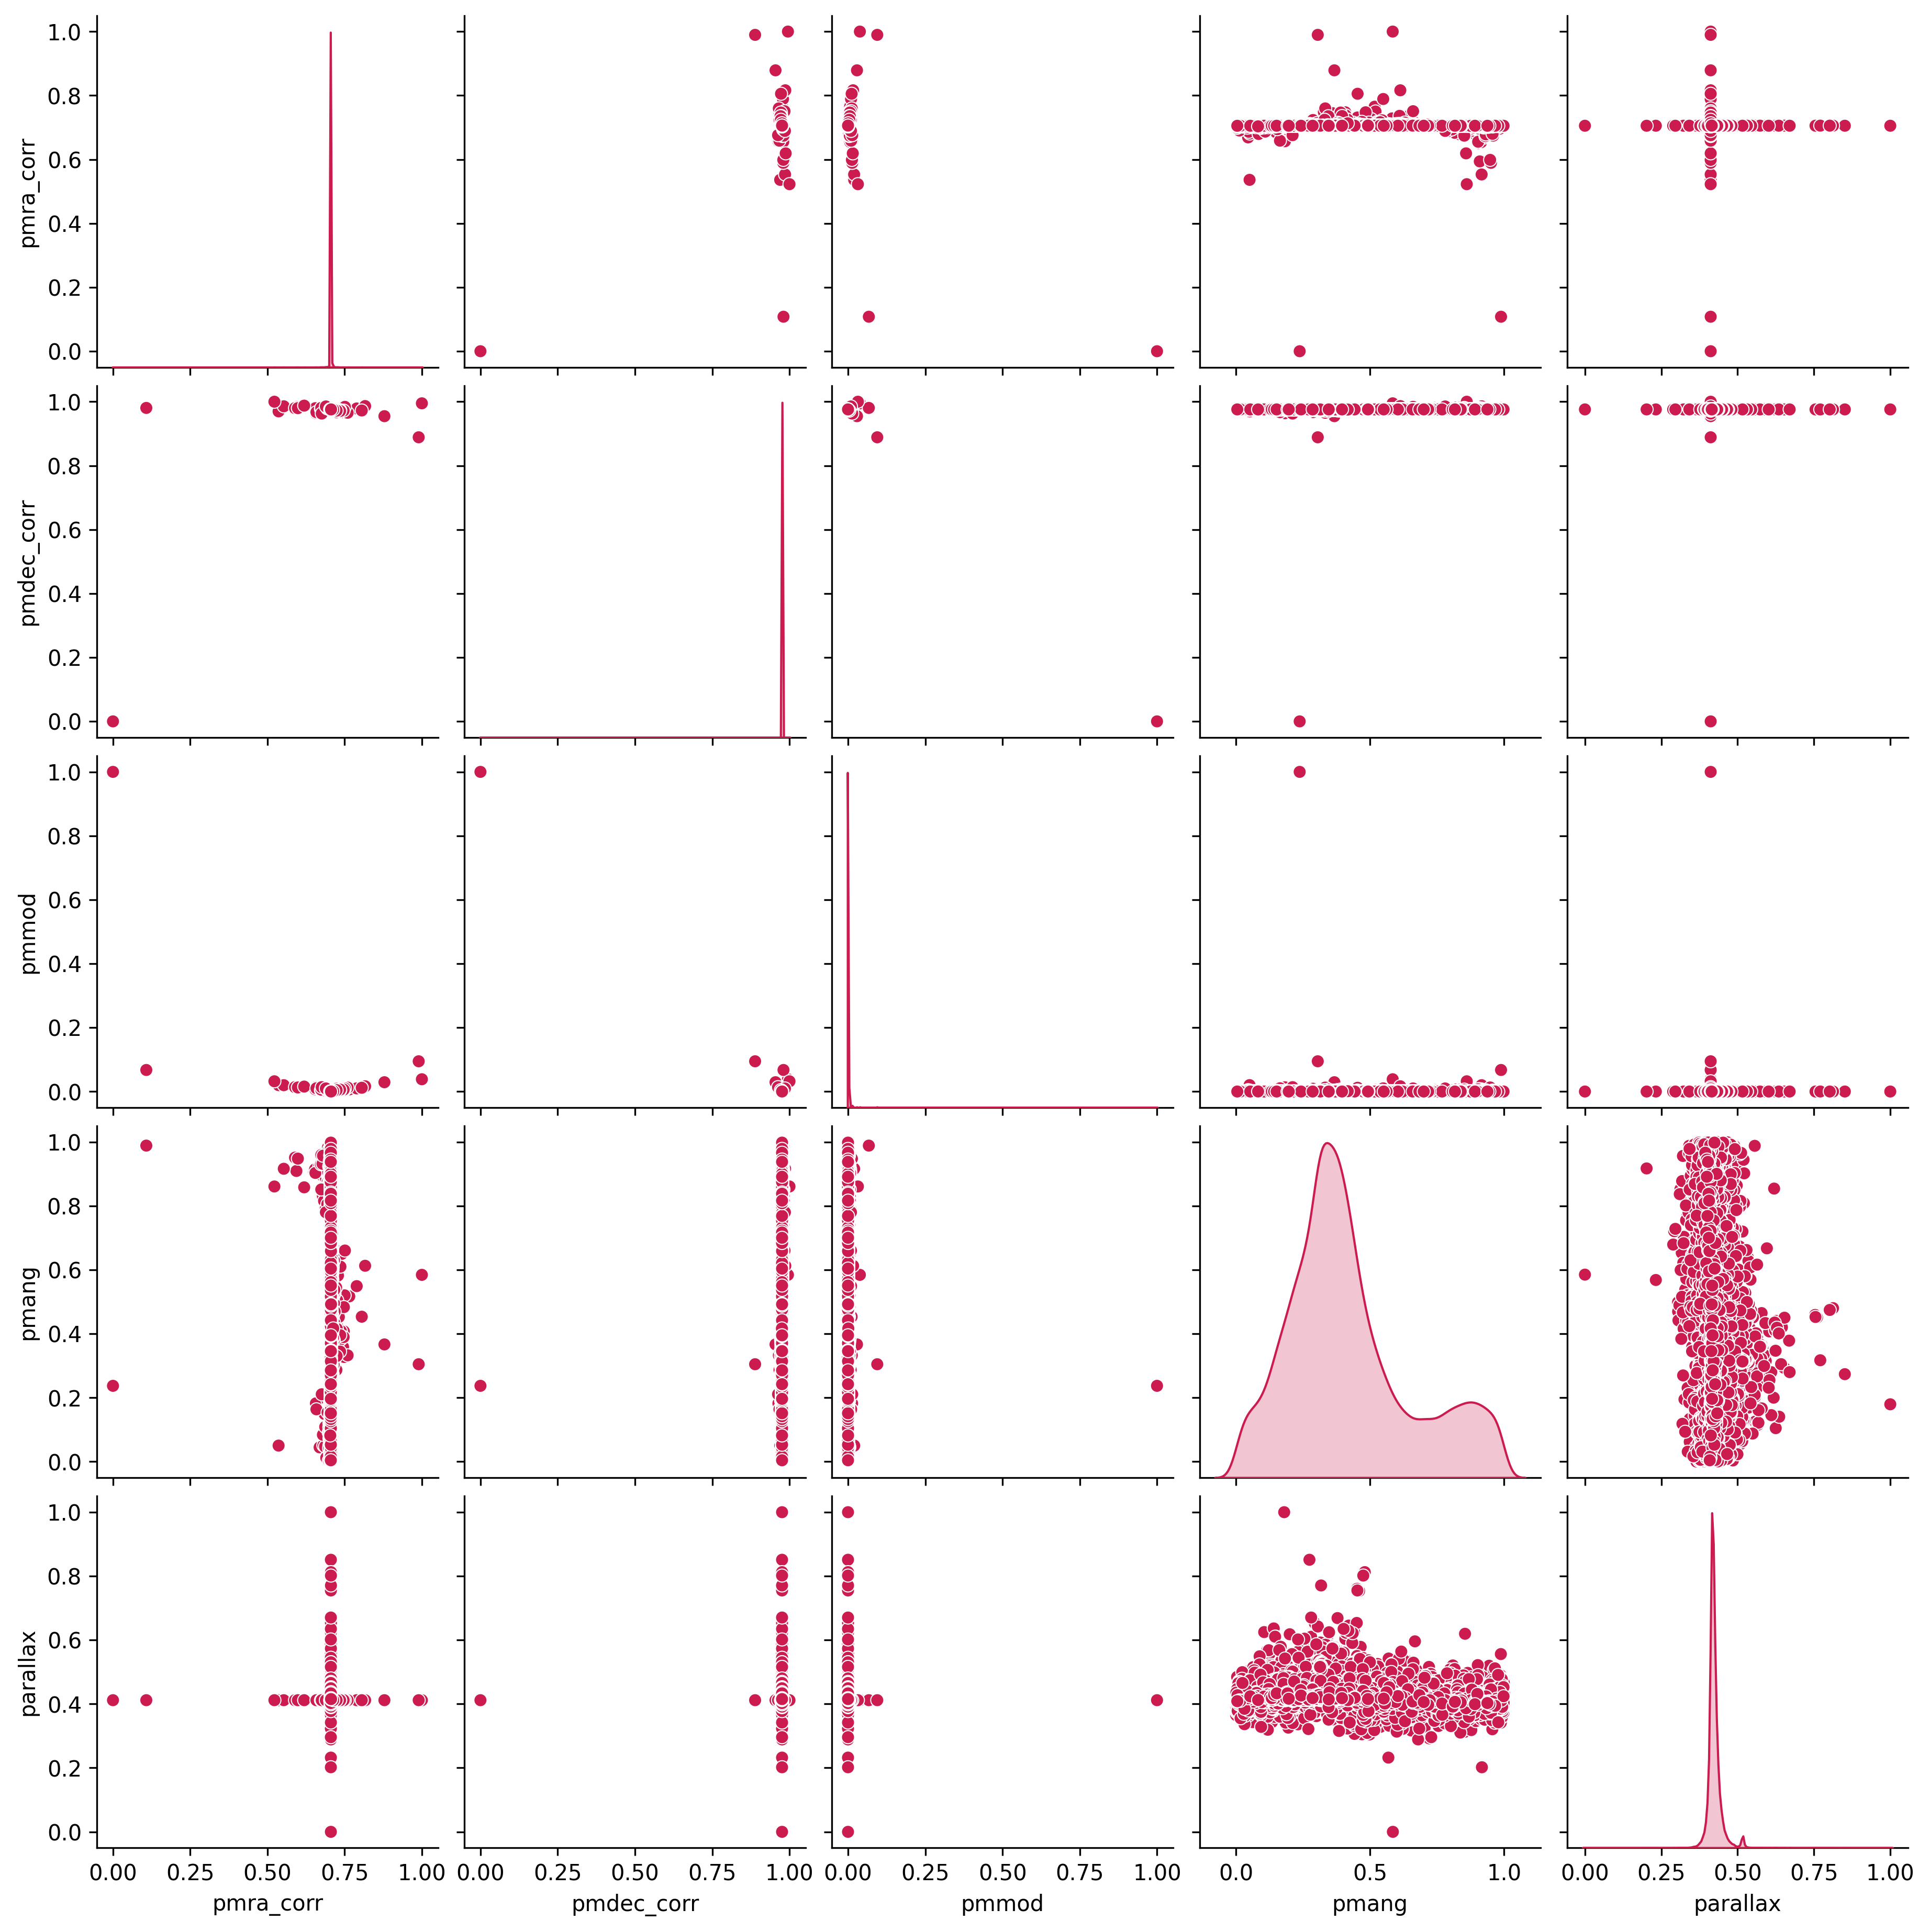
\includegraphics[scale=0.5]{../figures/melotte_22/features_melotte_22.png}
  \caption{Pairwise relationships among variables using Melotte 22 data}
  \label{fig:features_melotte_22}
\end{figure*}

First, we correct proper motion in right ascension and declination by dividing them by the parallax (variables pmra\_corr and pmdec\_corr, respectively). That way, we normalize these quantities and help our clustering models to improve their performance. The modulus of the proper motion (variable pmmod in Figure~\ref{fig:features_melotte_22}) is another computed property that we considered. We use it to relate both features and therefore force our model to keep them tight.

\subsection{Deep Open Clustering of Stars}
\label{sec:deep_open_clustering}

In this section, we explain our model in more detail.

One of the main problems to define our model is that we do not have a labeled dataset to train a supervised model. To solve it, we employ an unsupervised self-trained model. Thus, we adapted the Unsupervised \emph{DEC} model~\cite{xie2016unsupervised} to our requirements.

Like the DEC model, we have two main components:

\begin{itemize}
  \item \textbf{deep autoencoder:} it is a neural network that learns to copy its input to its output. It is composed of encoder layers followed by decoder layers. We trained it before passing the data through the next component, the \emph{clustering layer}. Recent research~\cite{vincent2010stacked,hinton2006reducing} showed that the autoencoder provides meaningful and well-separated representations on real-world datasets.
  \item \textbf{clustering layer:} it receives data transformed by the autoencoder and iteratively is trained until a convergence criterion is met.
\end{itemize}

The deep autoencoder is used to transform the input data into a latent space using a non-linear mapping function \(f_{\theta} : X \rightarrow Z\).

We trained the autoencoder before fitting the model to generate predictions. Then, we use the encoder layers of the autoencoder with the aim of transforming input data to the latent space \(Z\). Once the data has been transformed, a K-Means clusterer is used to make an initial clustering. K-Means cluster centers are used as the initial weights for the clustering layer.

With that initial configuration, the model iterates alternating between computing an auxiliary target distribution (soft assignment) and minimizing the Kullback-Leiber (KL) divergence~\cite{kullback1951information} to it. This unsupervised algorithm allows us to improve the clustering.

As it was described in Section~\ref{sec:feature_selection}, the number of features we deal is not too large. However, this latent space helps us to start with a reduced number of features and avoids the \emph{``curse of dimensionality''}~\cite{bellman1961curse}.

In the soft assignment stage, we used \emph{Student's t-distribution} as a kernel to measure the similarity between the embedded points and the cluster centroid. While in the KL divergence minimization the algorithm iteratively refines clusters by learning from their high confidence assignments with the help of an auxiliary target distribution. The model is trained by matching the soft assignment to the target distribution. The choice of this target distribution is crucial for model's performance.

In this work, we took the target distribution~\cite{xie2016unsupervised} defined in Equation~\ref{eq:student_tdistribution}.

\begin{equation}
  p_{ij} = \frac{q^{2}_{ij} / f_{j}}{\sum_{j'}q^{2}_{ij'}/f_{j'}}
  \label{eq:student_tdistribution}
\end{equation}

This target distribution has the following properties:

\begin{itemize}
  \item strengthen predictions (i.e., improve cluster purity),
  \item put more emphasis on data points assigned with high confidence,
  \item normalize loss contribution of each centroid to prevent large clusters from distorting the hidden feature space.
\end{itemize}

\begin{figure*}[!hbt]
  \centering
  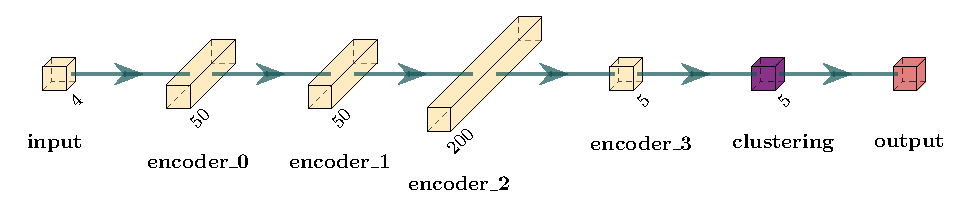
\includegraphics[scale=0.8]{../figures/dec_diagram.pdf}
  \caption{Layer setup of our model}
  \label{fig:dec_model_setup}
\end{figure*}

Figure~\ref{fig:dec_model_setup} shows the layer setup of our model. It is simpler than the used in~\cite{xie2016unsupervised} because we selected a smaller number of features. Therefore, using the same configuration would result in a model so powerful that it would incur overfitting issues that cannot make the correct predictions.

\begin{figure*}[!htbp]
  \centering
  \begin{subfigure}[b]{0.3\textwidth}
    \centering
      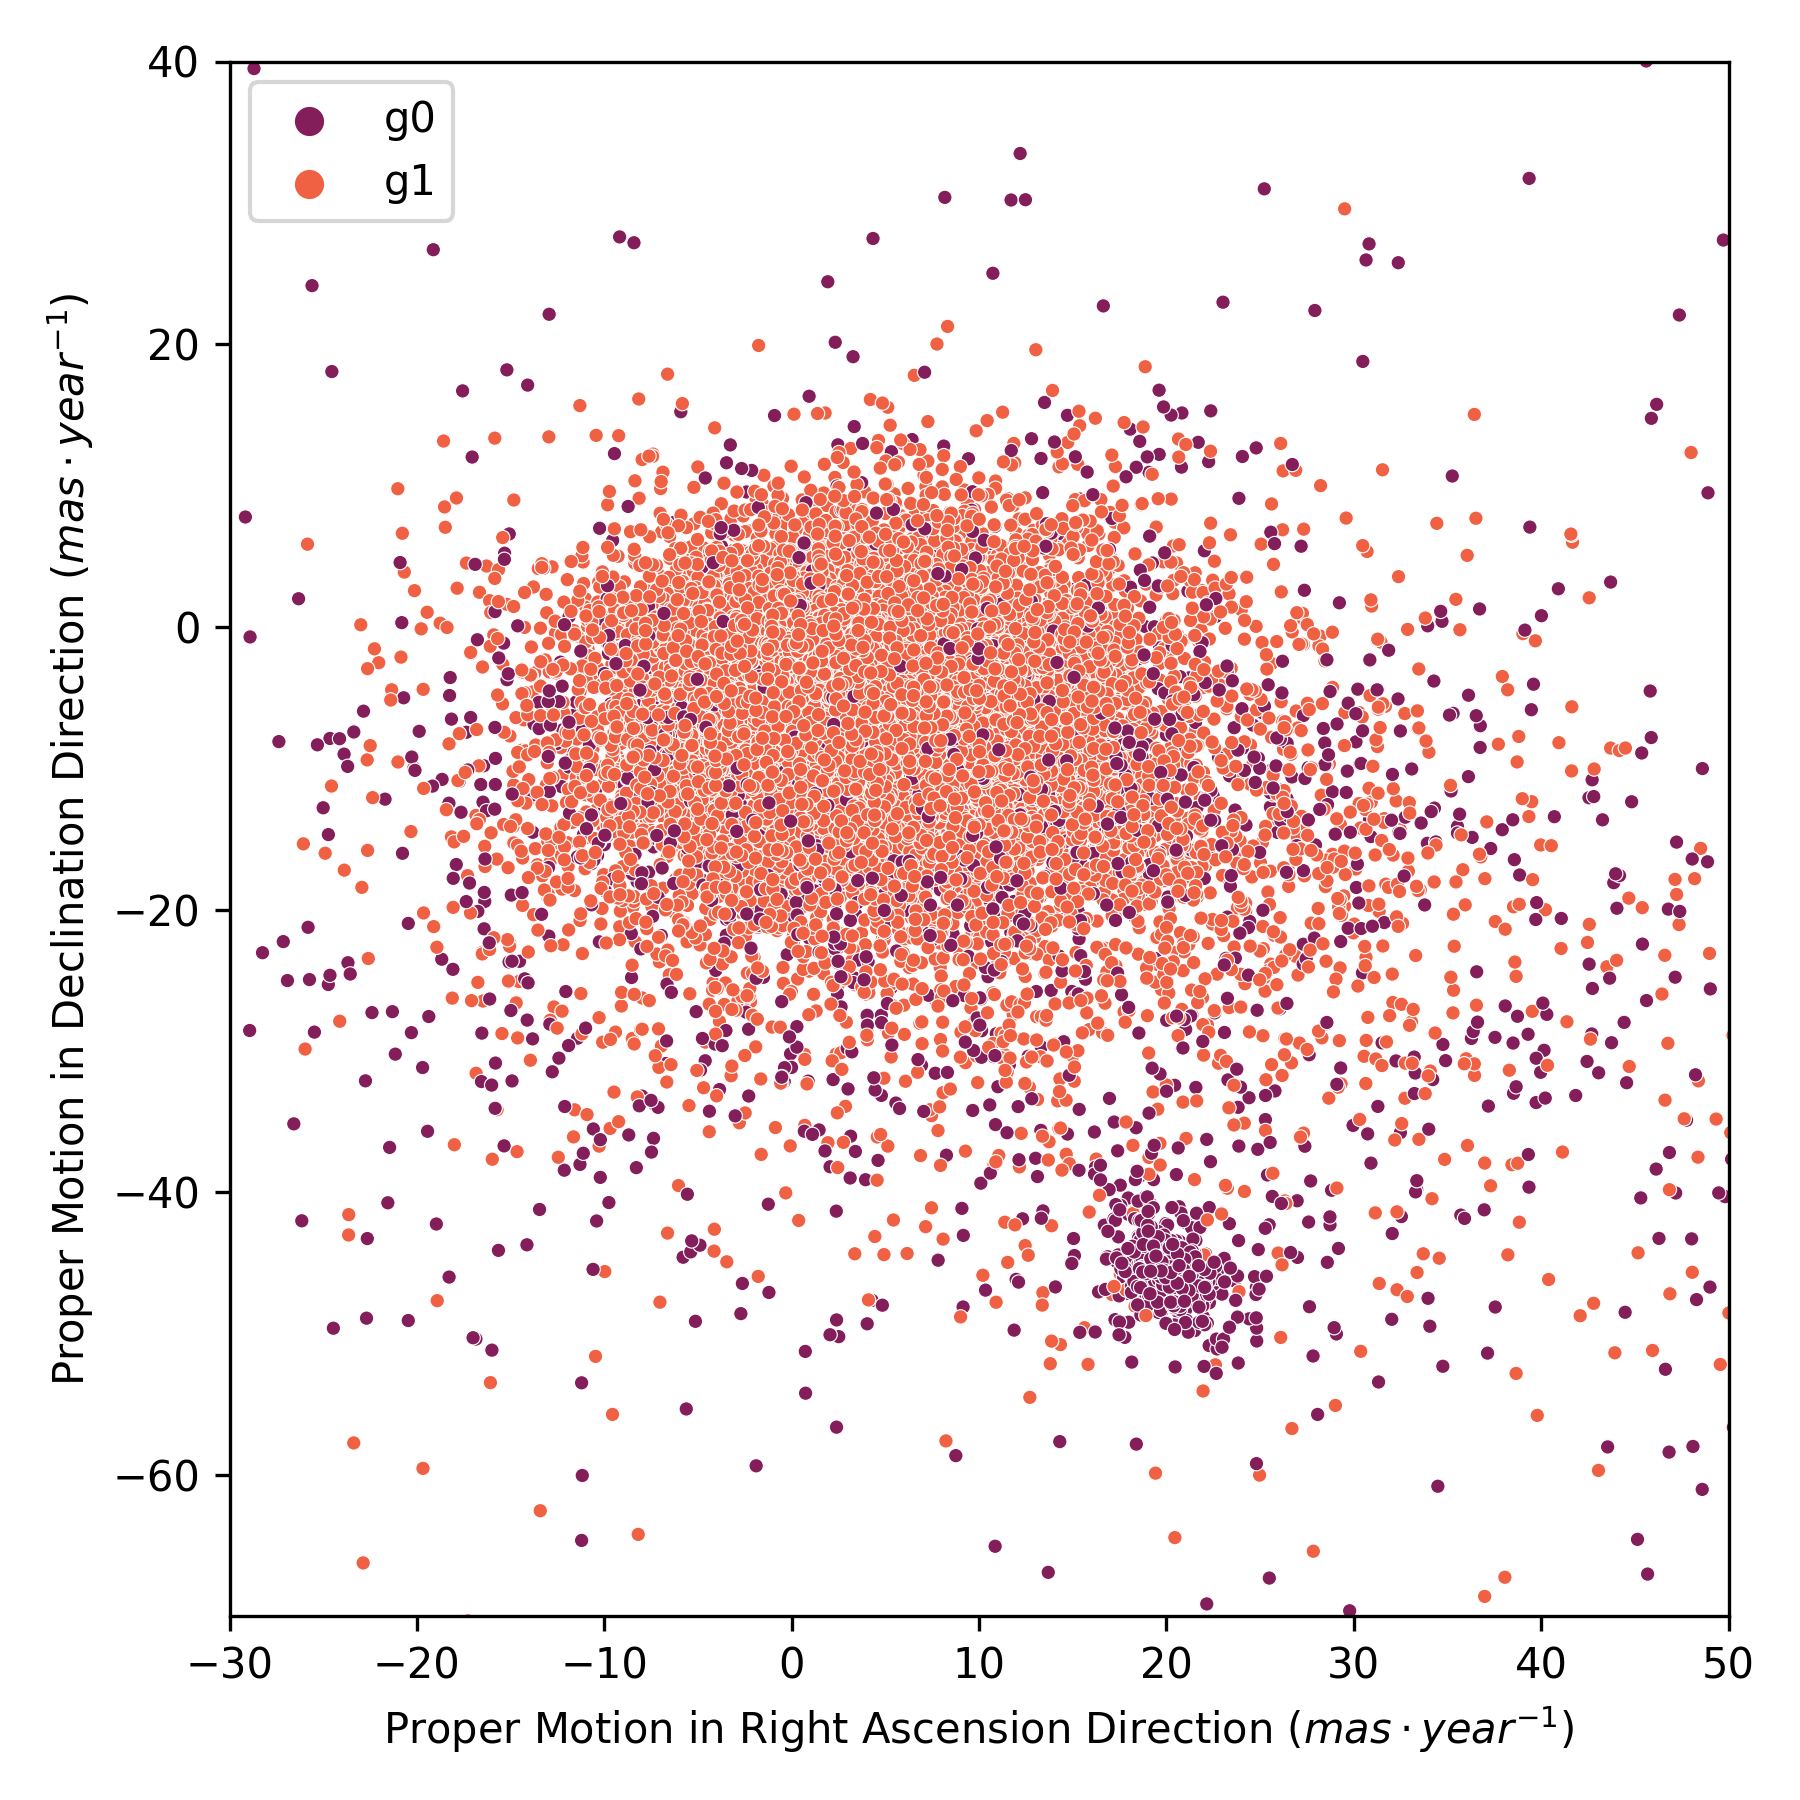
\includegraphics[width=\textwidth]{../figures/kmeans/kmeans_n2_pm_melotte_22.png}
      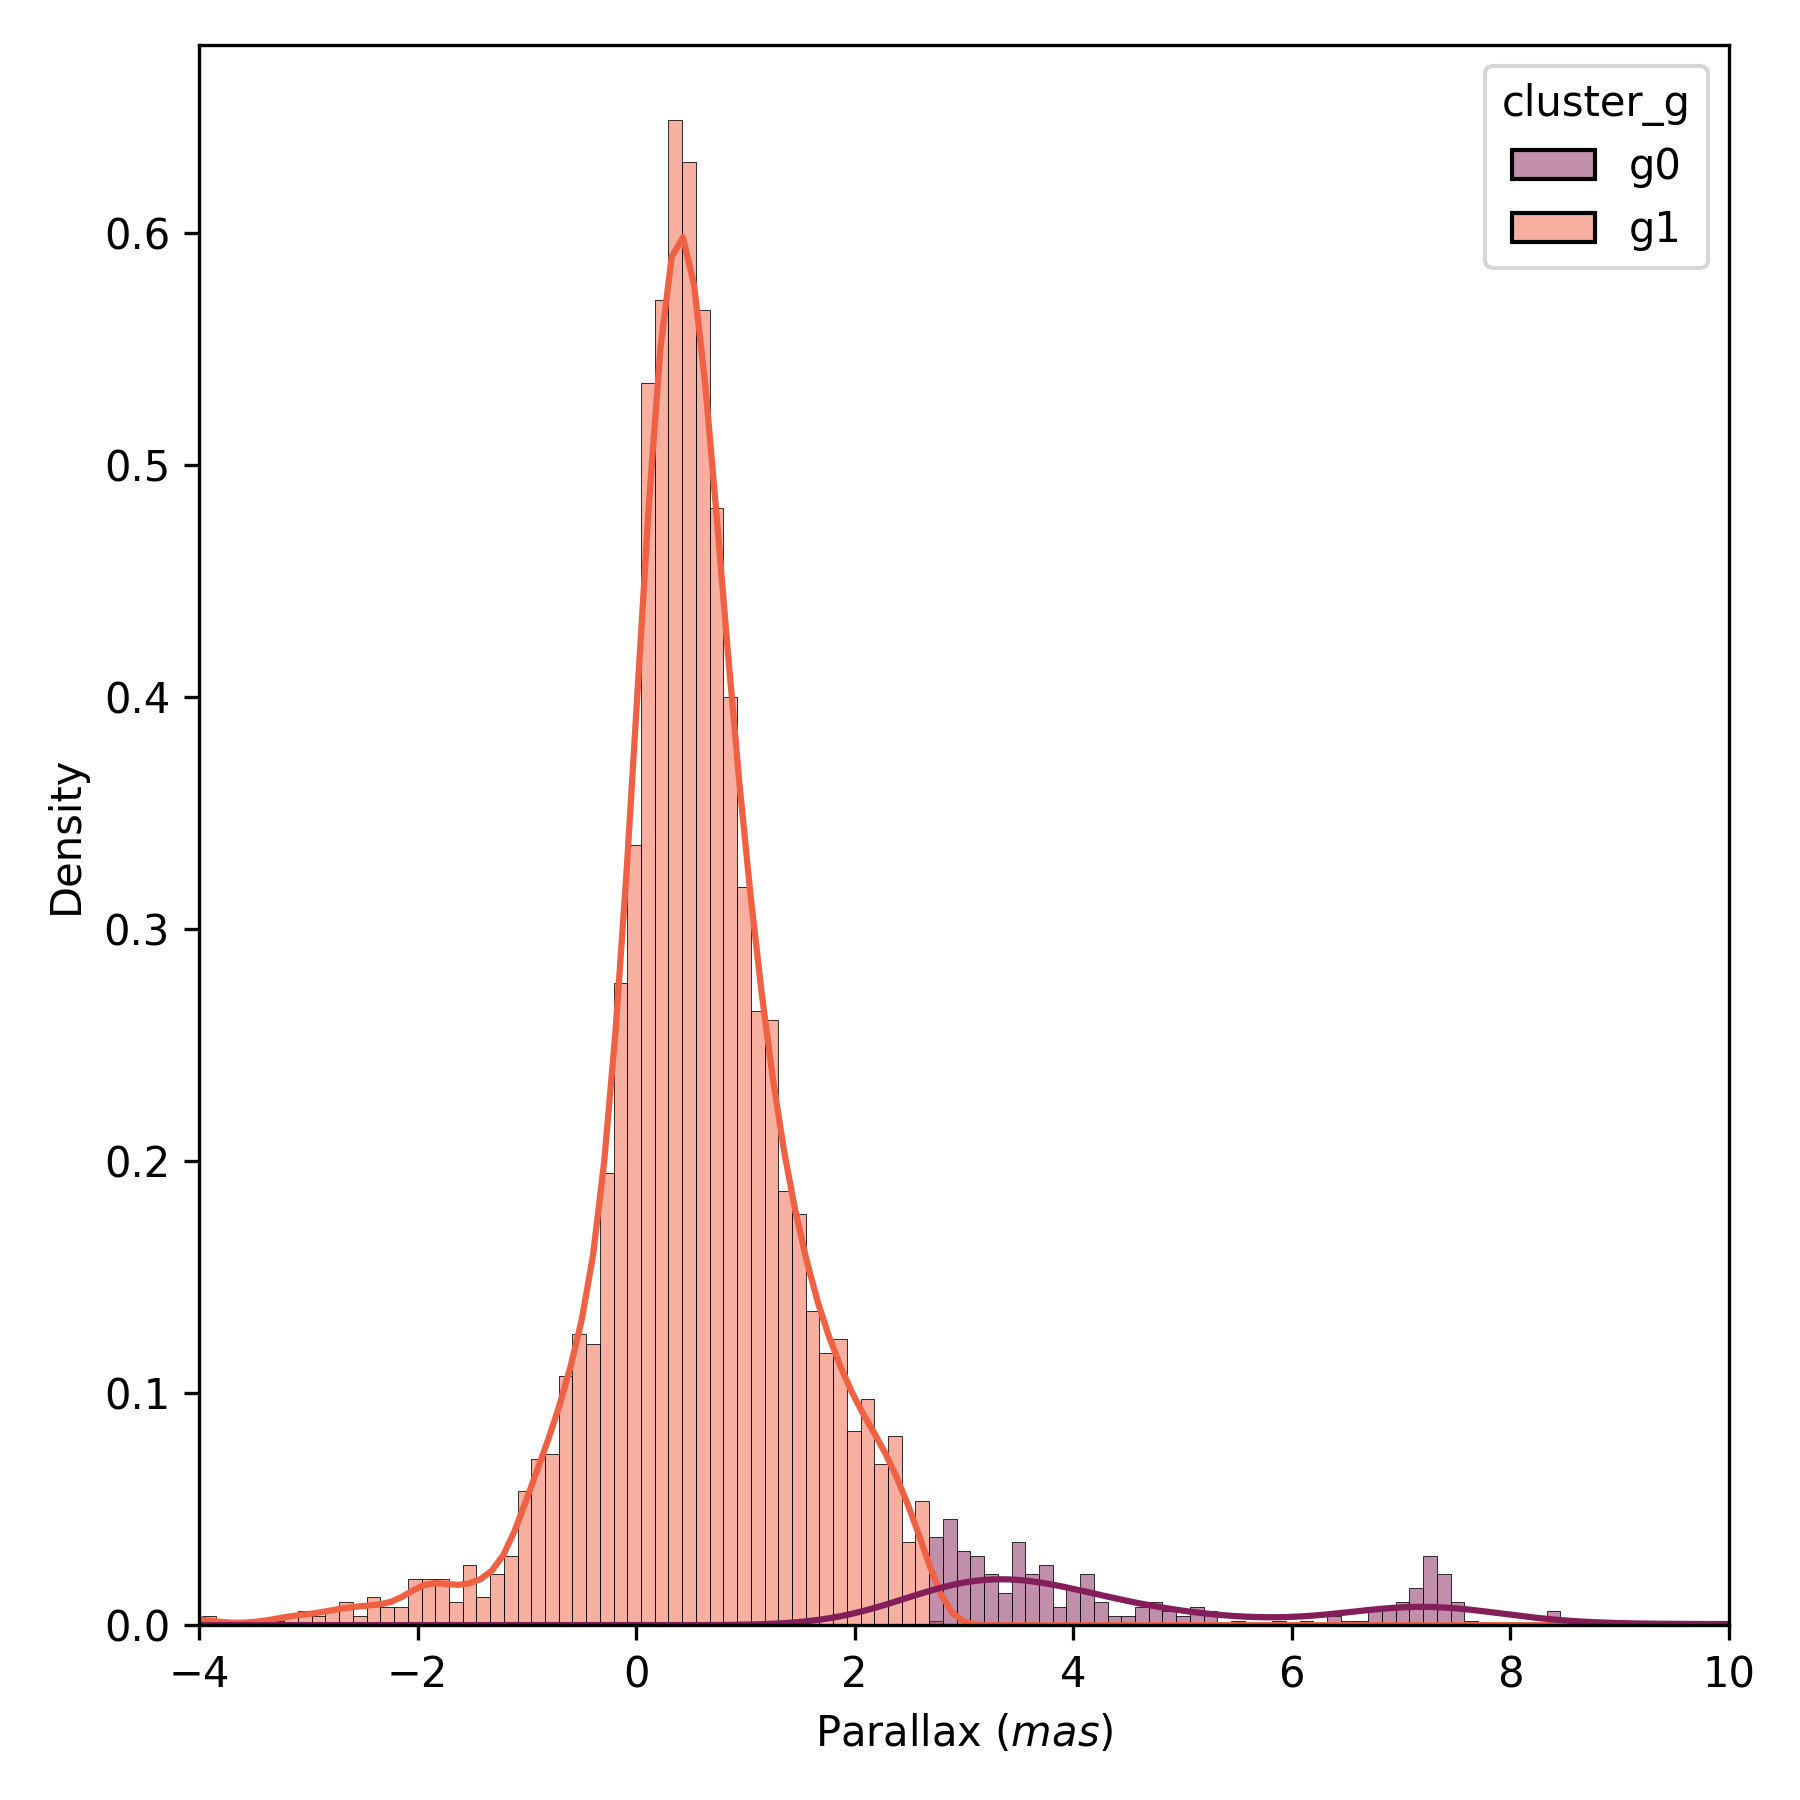
\includegraphics[width=\textwidth]{../figures/kmeans/kmeans_n2_parallax_melotte_22.png}
      \caption{N = 2}
  \end{subfigure}
  \medskip
  \begin{subfigure}[b]{0.3\textwidth}
    \centering
      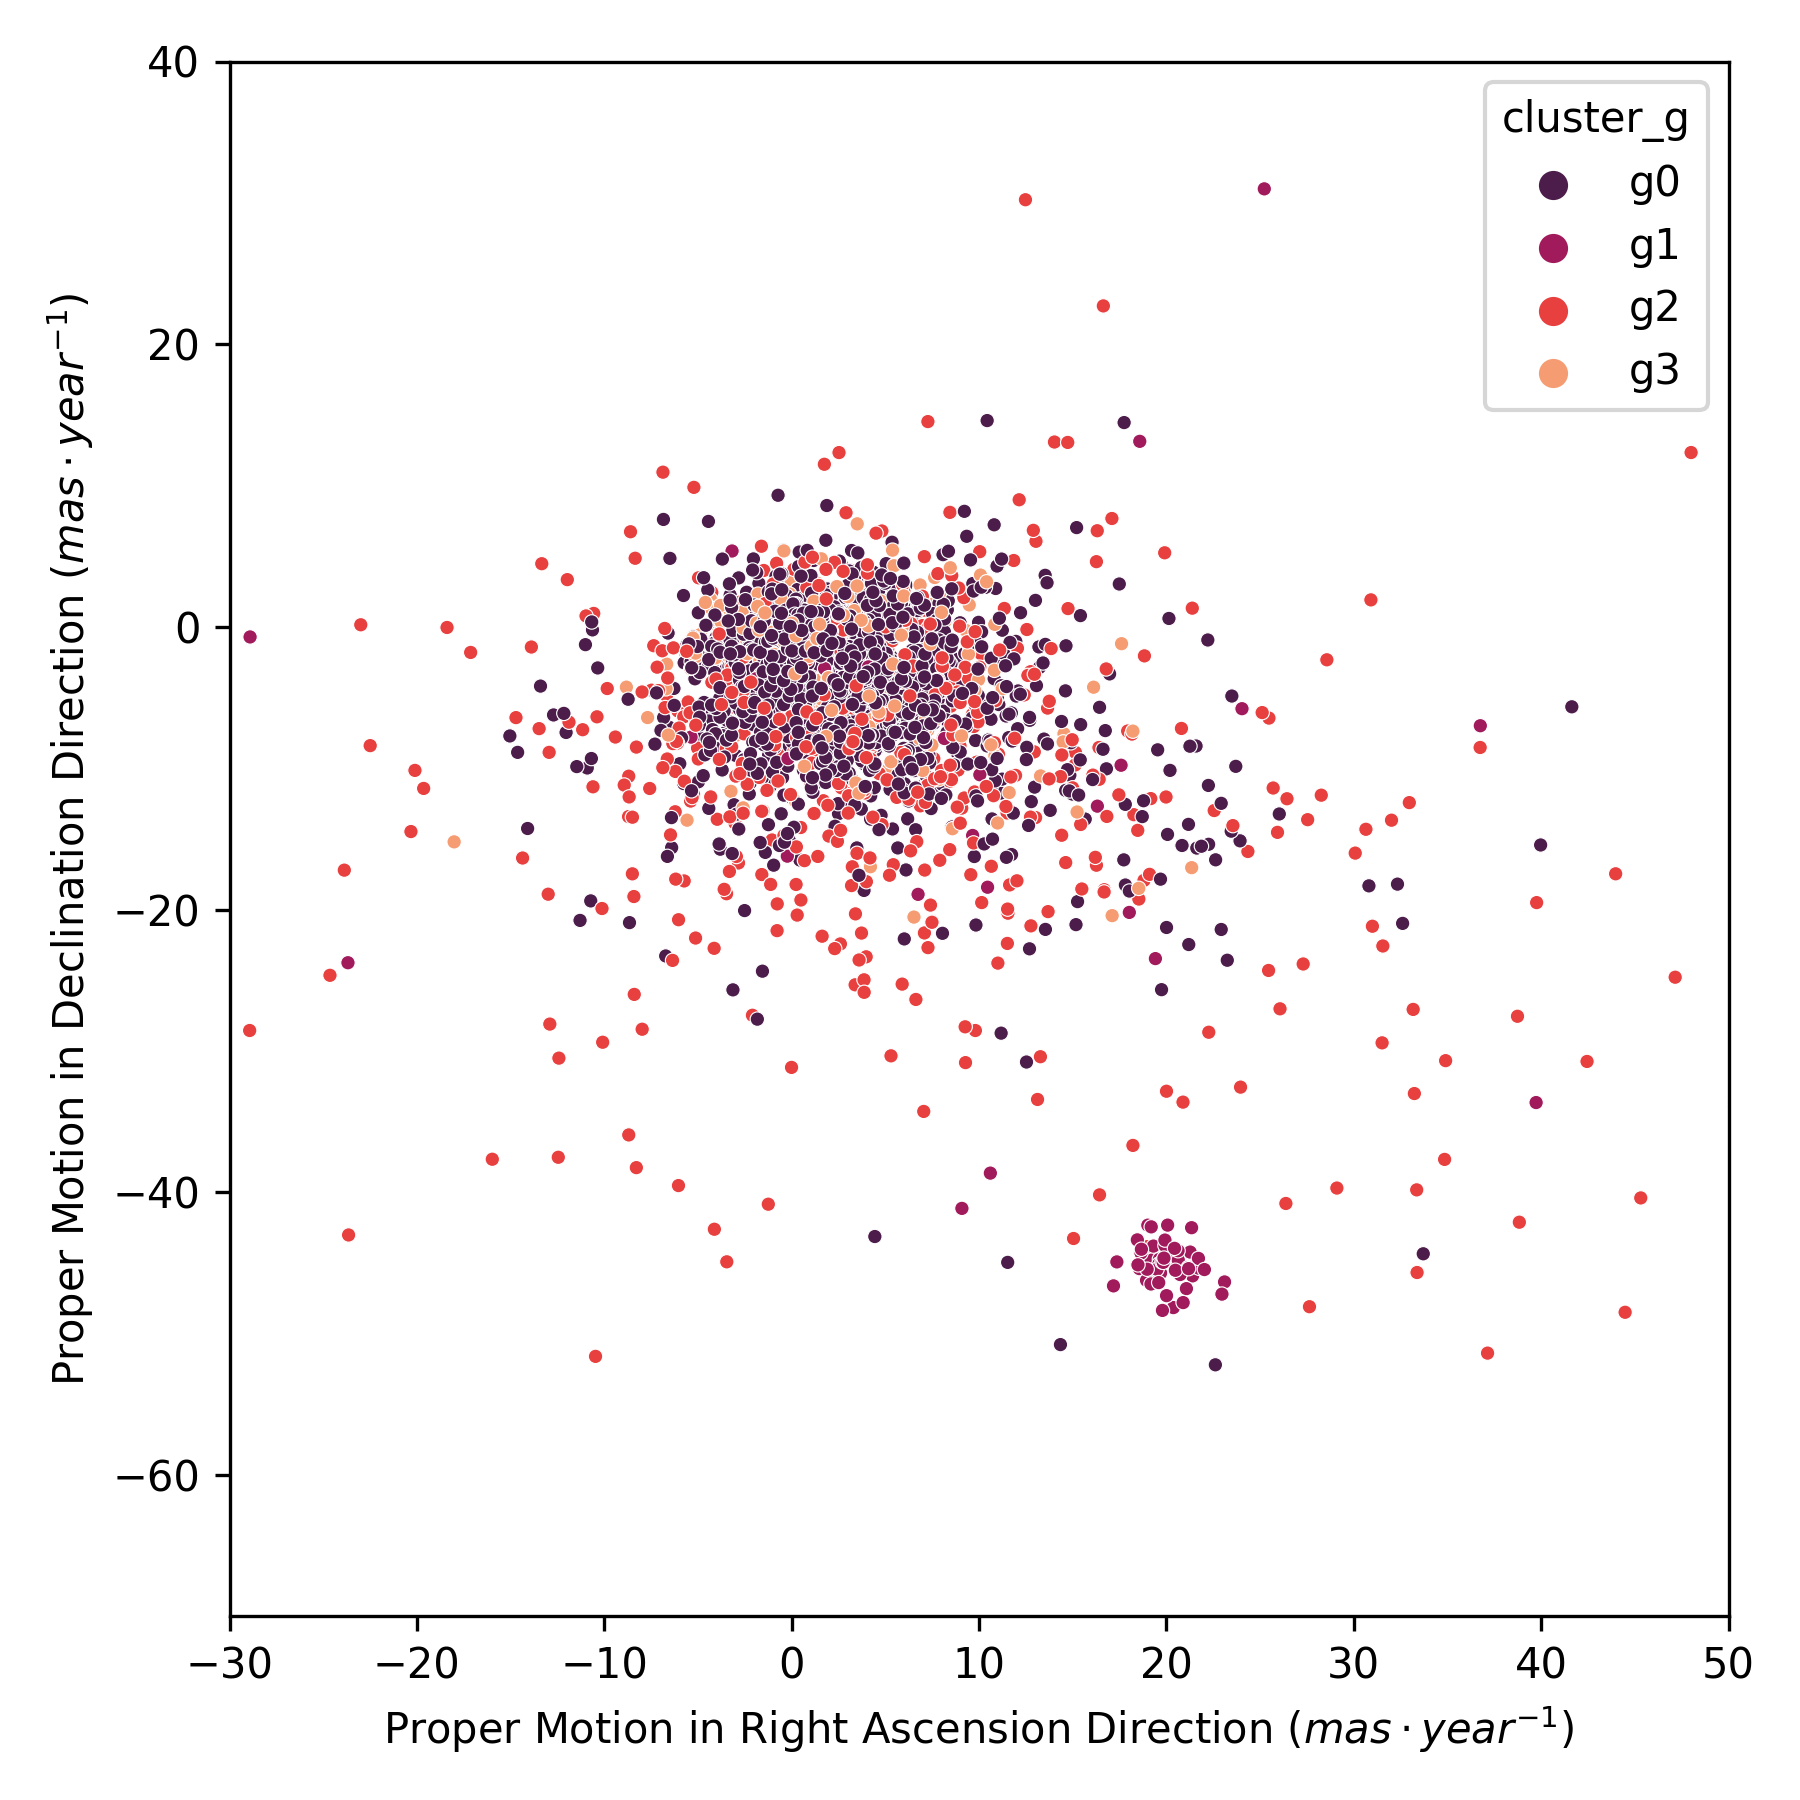
\includegraphics[width=\textwidth]{../figures/kmeans/kmeans_n5_pm_melotte_22.png}
      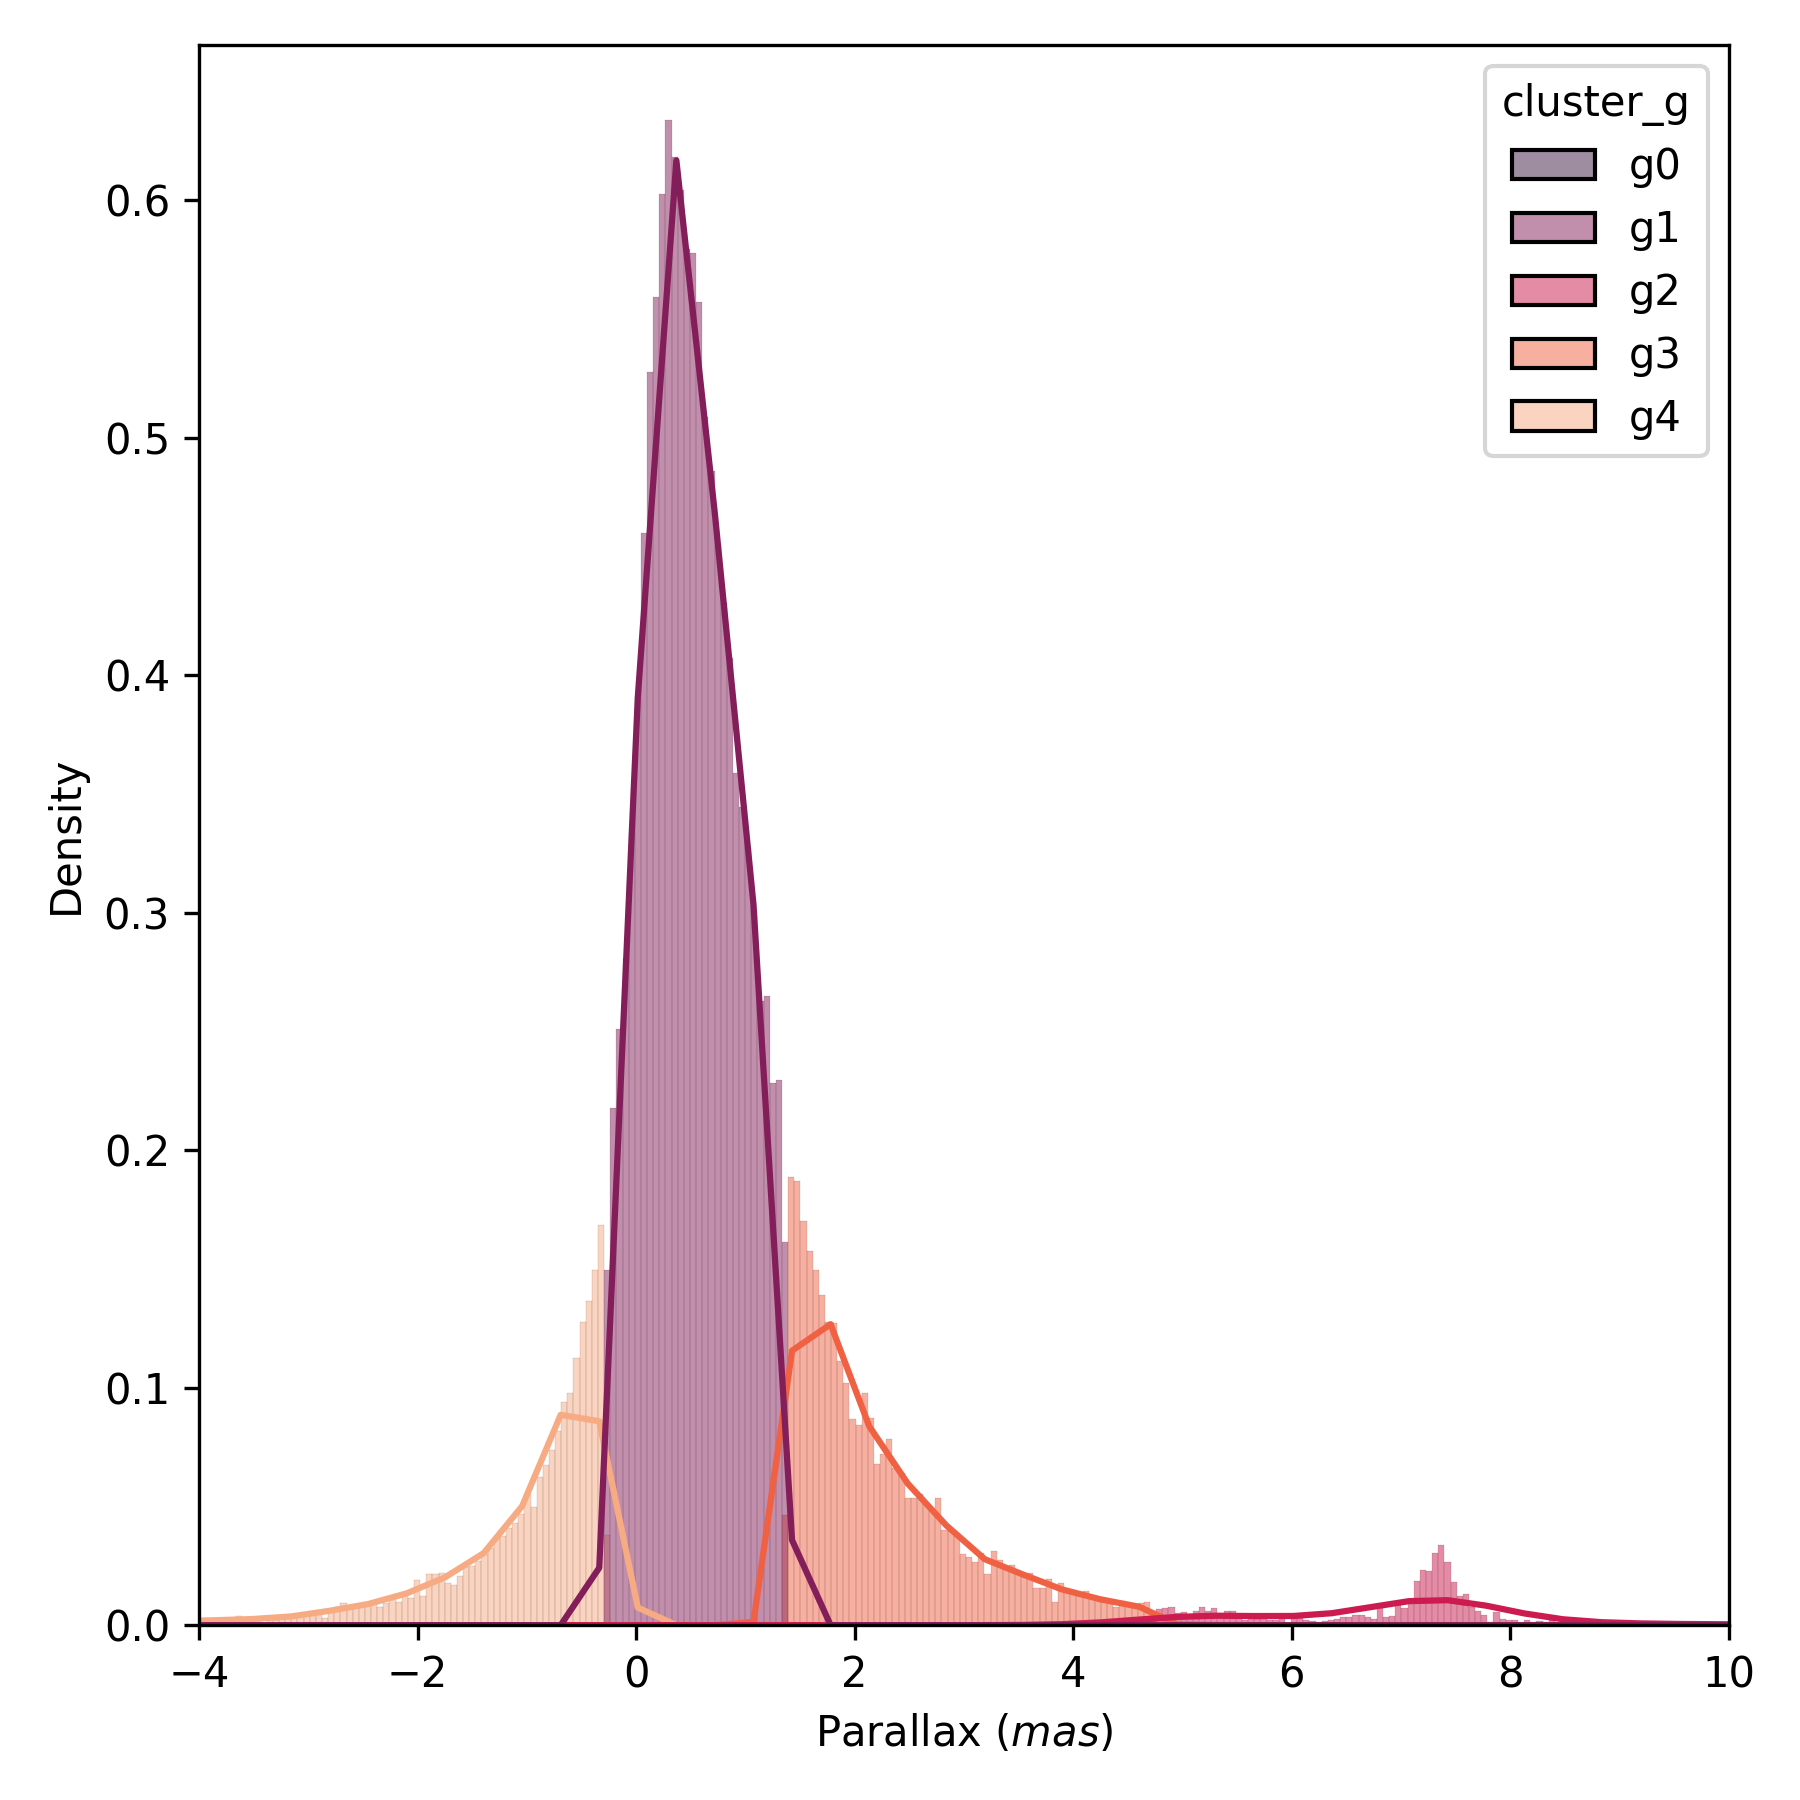
\includegraphics[width=\textwidth]{../figures/kmeans/kmeans_n5_parallax_melotte_22.png}
      \caption{N = 5}
  \end{subfigure}
  \medskip
  \begin{subfigure}[b]{0.3\textwidth}
    \centering
      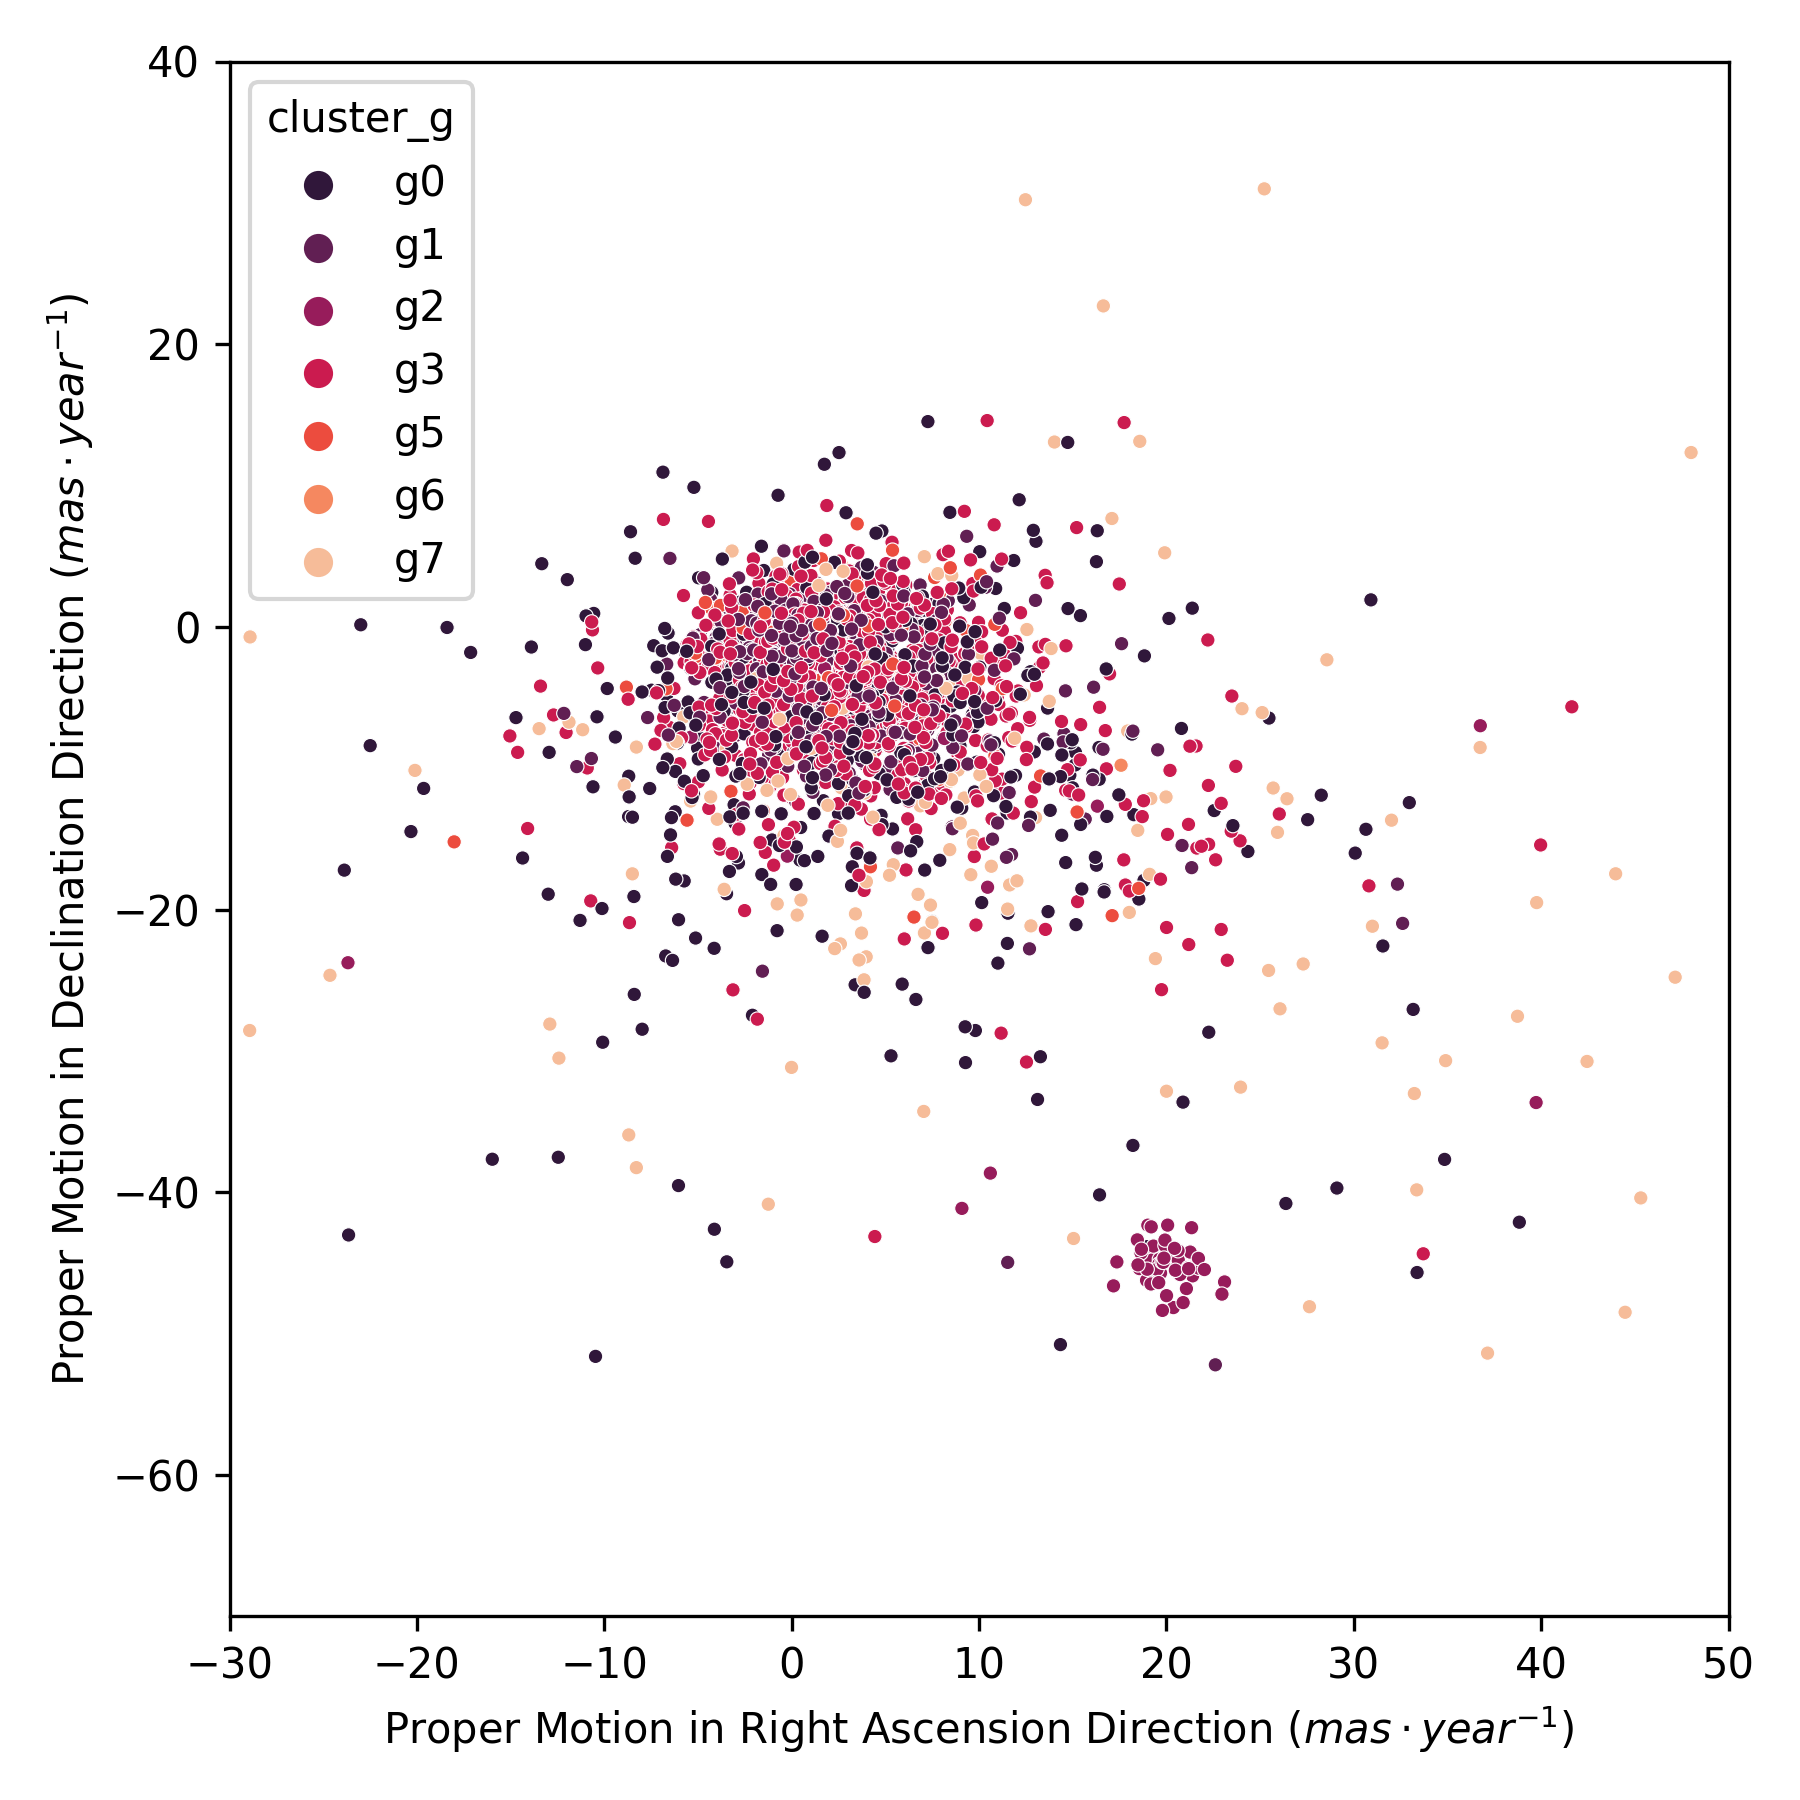
\includegraphics[width=\textwidth]{../figures/kmeans/kmeans_n8_pm_melotte_22.png}
      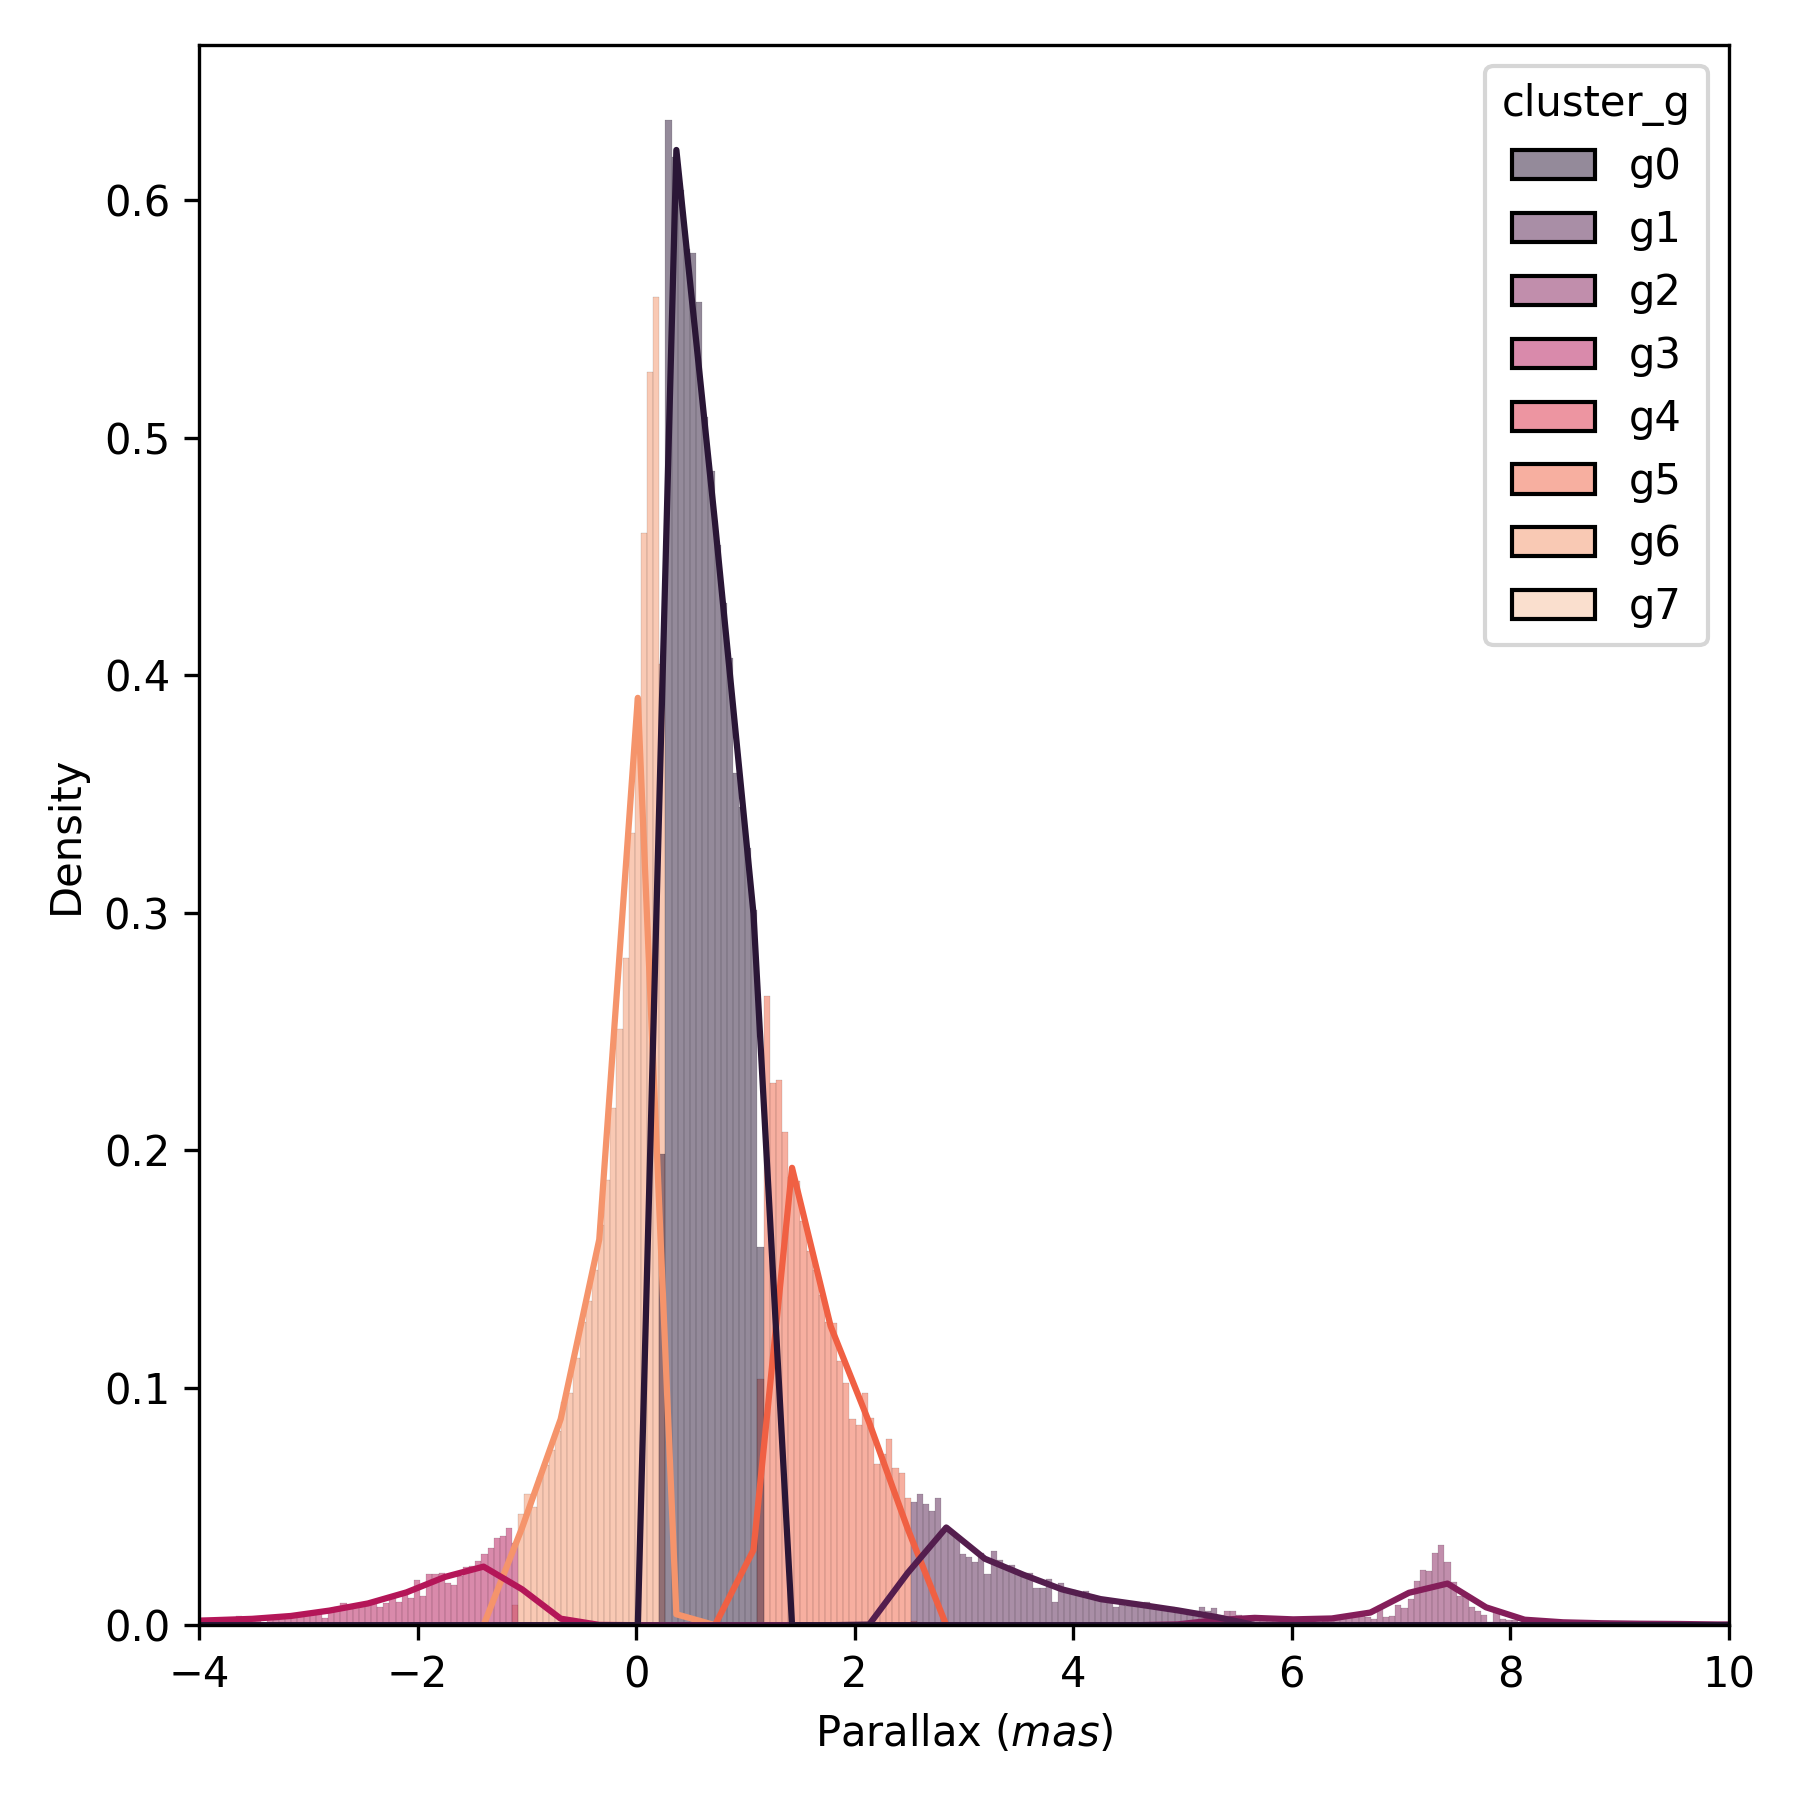
\includegraphics[width=\textwidth]{../figures/kmeans/kmeans_n8_parallax_melotte_22.png}
      \caption{N = 8}
  \end{subfigure}
  \caption{K-Means with Melotte 22}
  \label{fig:kmeans_comparisons_melotte_22}
\end{figure*}

Finally, we can refine this selection by filtering those stars that are below and above the 0.10 and 0.90 quantiles for each group, respectively. That way we remove the most doubtful values from the selection.

\paragraph{Discussion.}

%% Comparación con K-Means, DEC y DEC filter
\begin{figure*}[!htbp]
  \centering
  \begin{subfigure}[b]{0.3\textwidth}
    \centering
      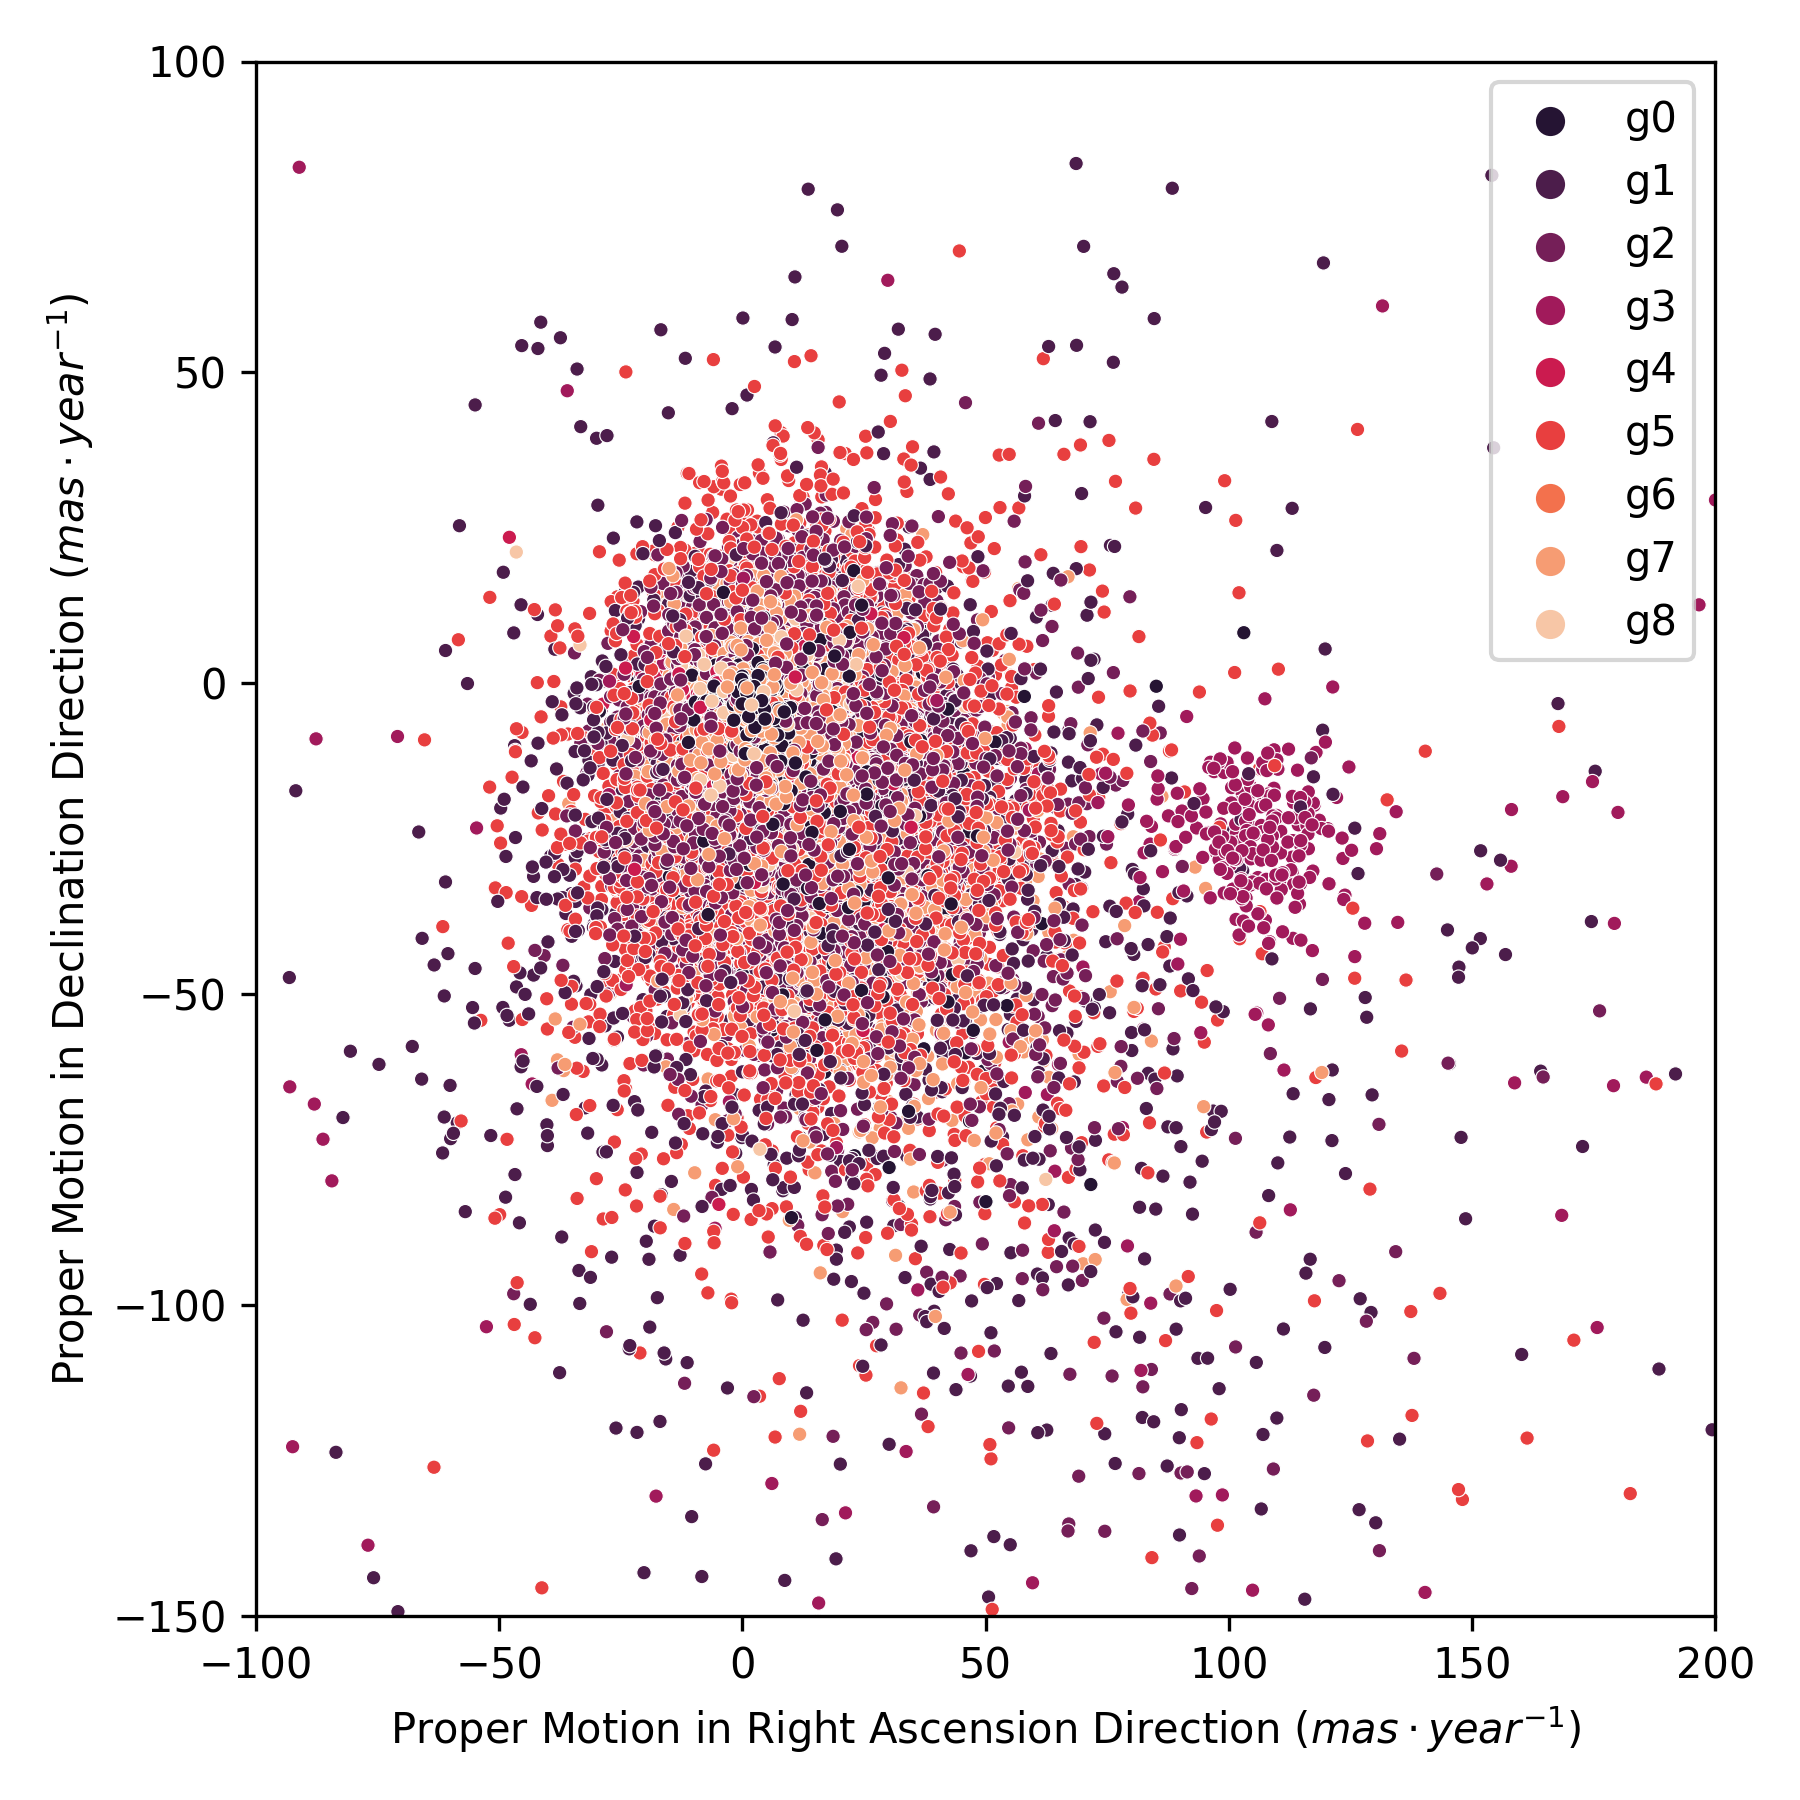
\includegraphics[width=\textwidth]{../figures/melotte_25/kmeans_pm_melotte_25.png}
      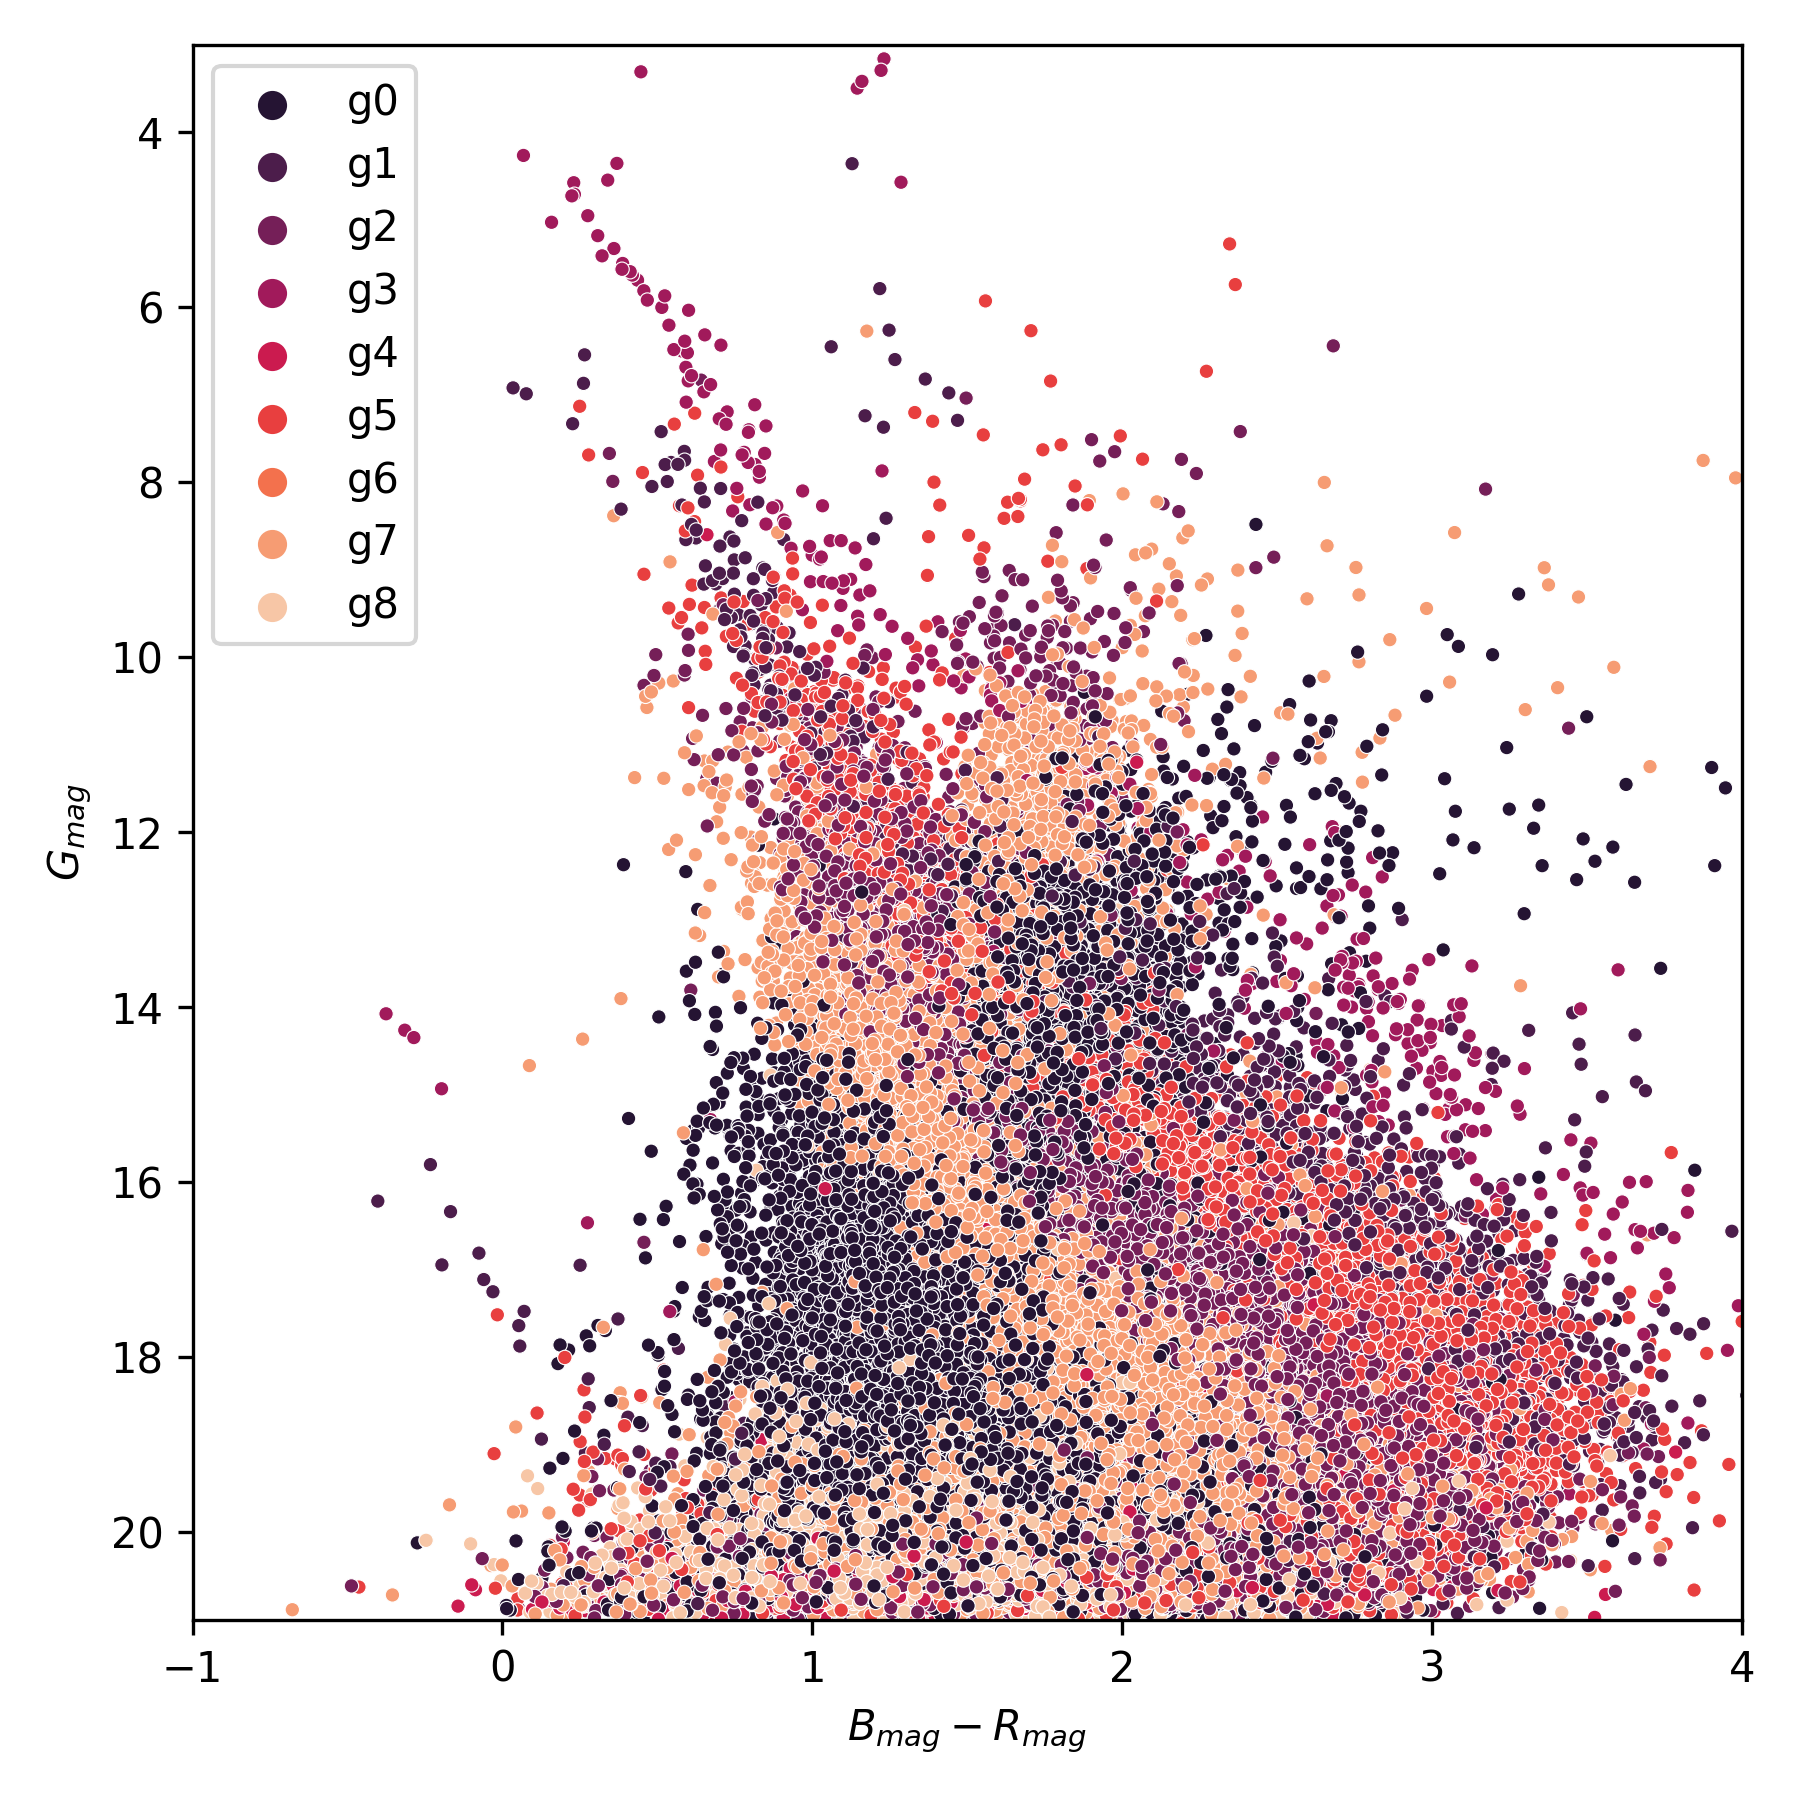
\includegraphics[width=\textwidth]{../figures/melotte_25/kmeans_hr_diagram_melotte_25.png}
      \caption{K-Means}
  \end{subfigure}
  \medskip
  \begin{subfigure}[b]{0.3\textwidth}
    \centering
      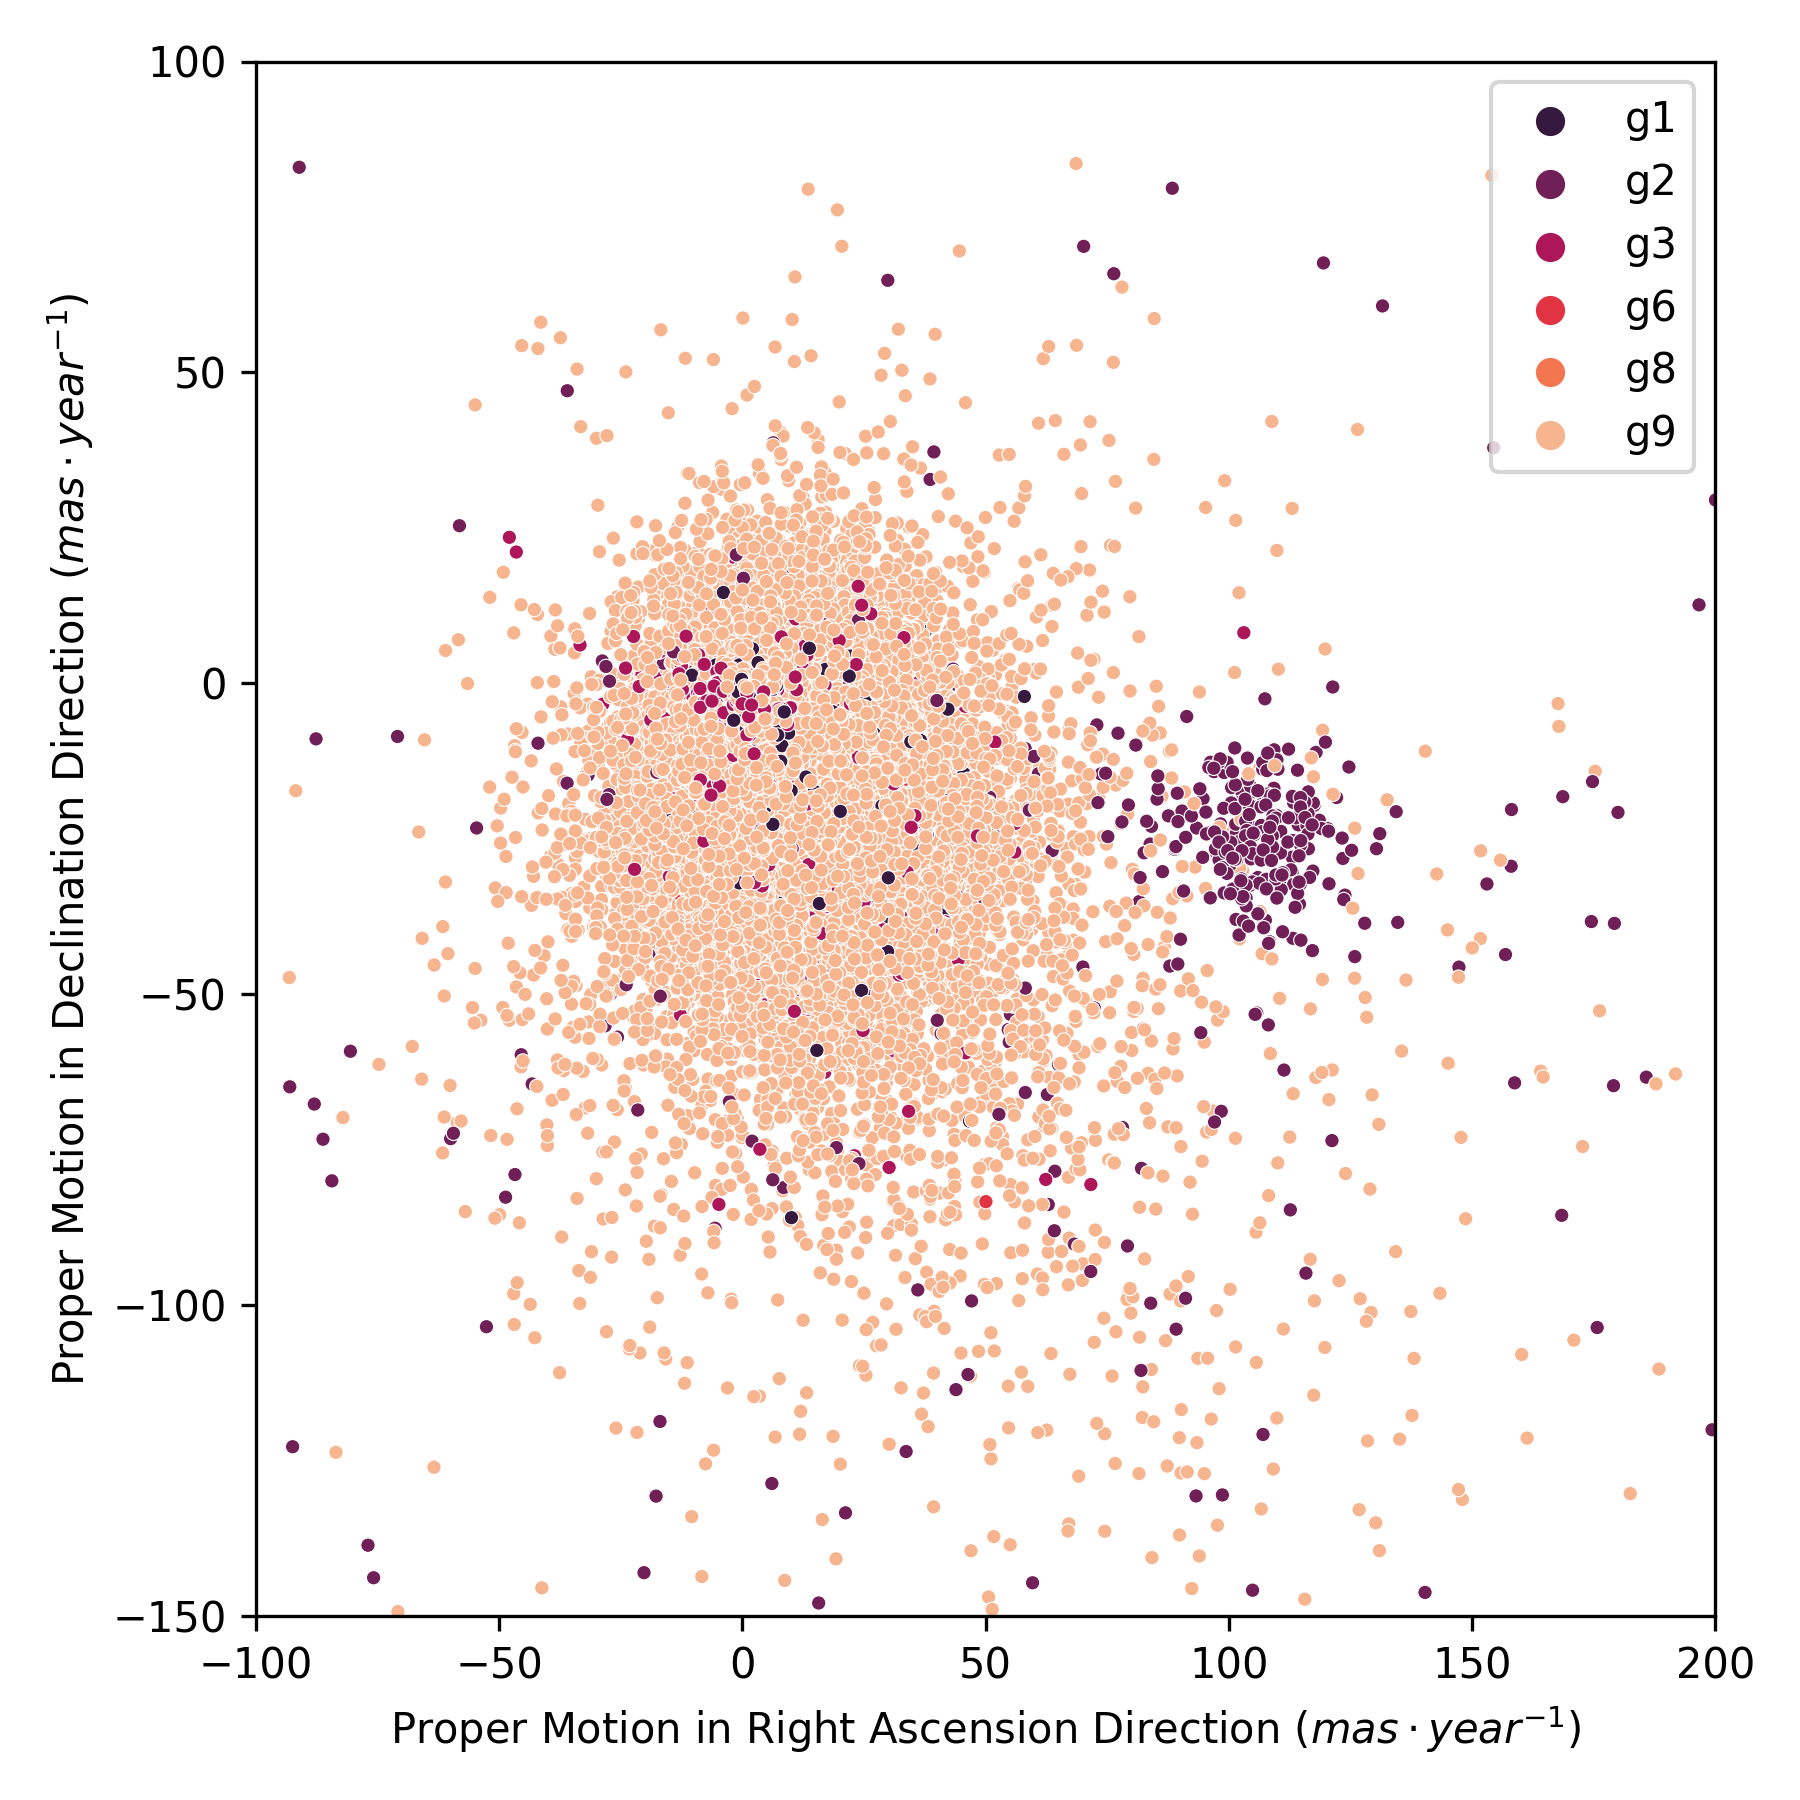
\includegraphics[width=\textwidth]{../figures/melotte_25/dec_pm_melotte_25.png}
      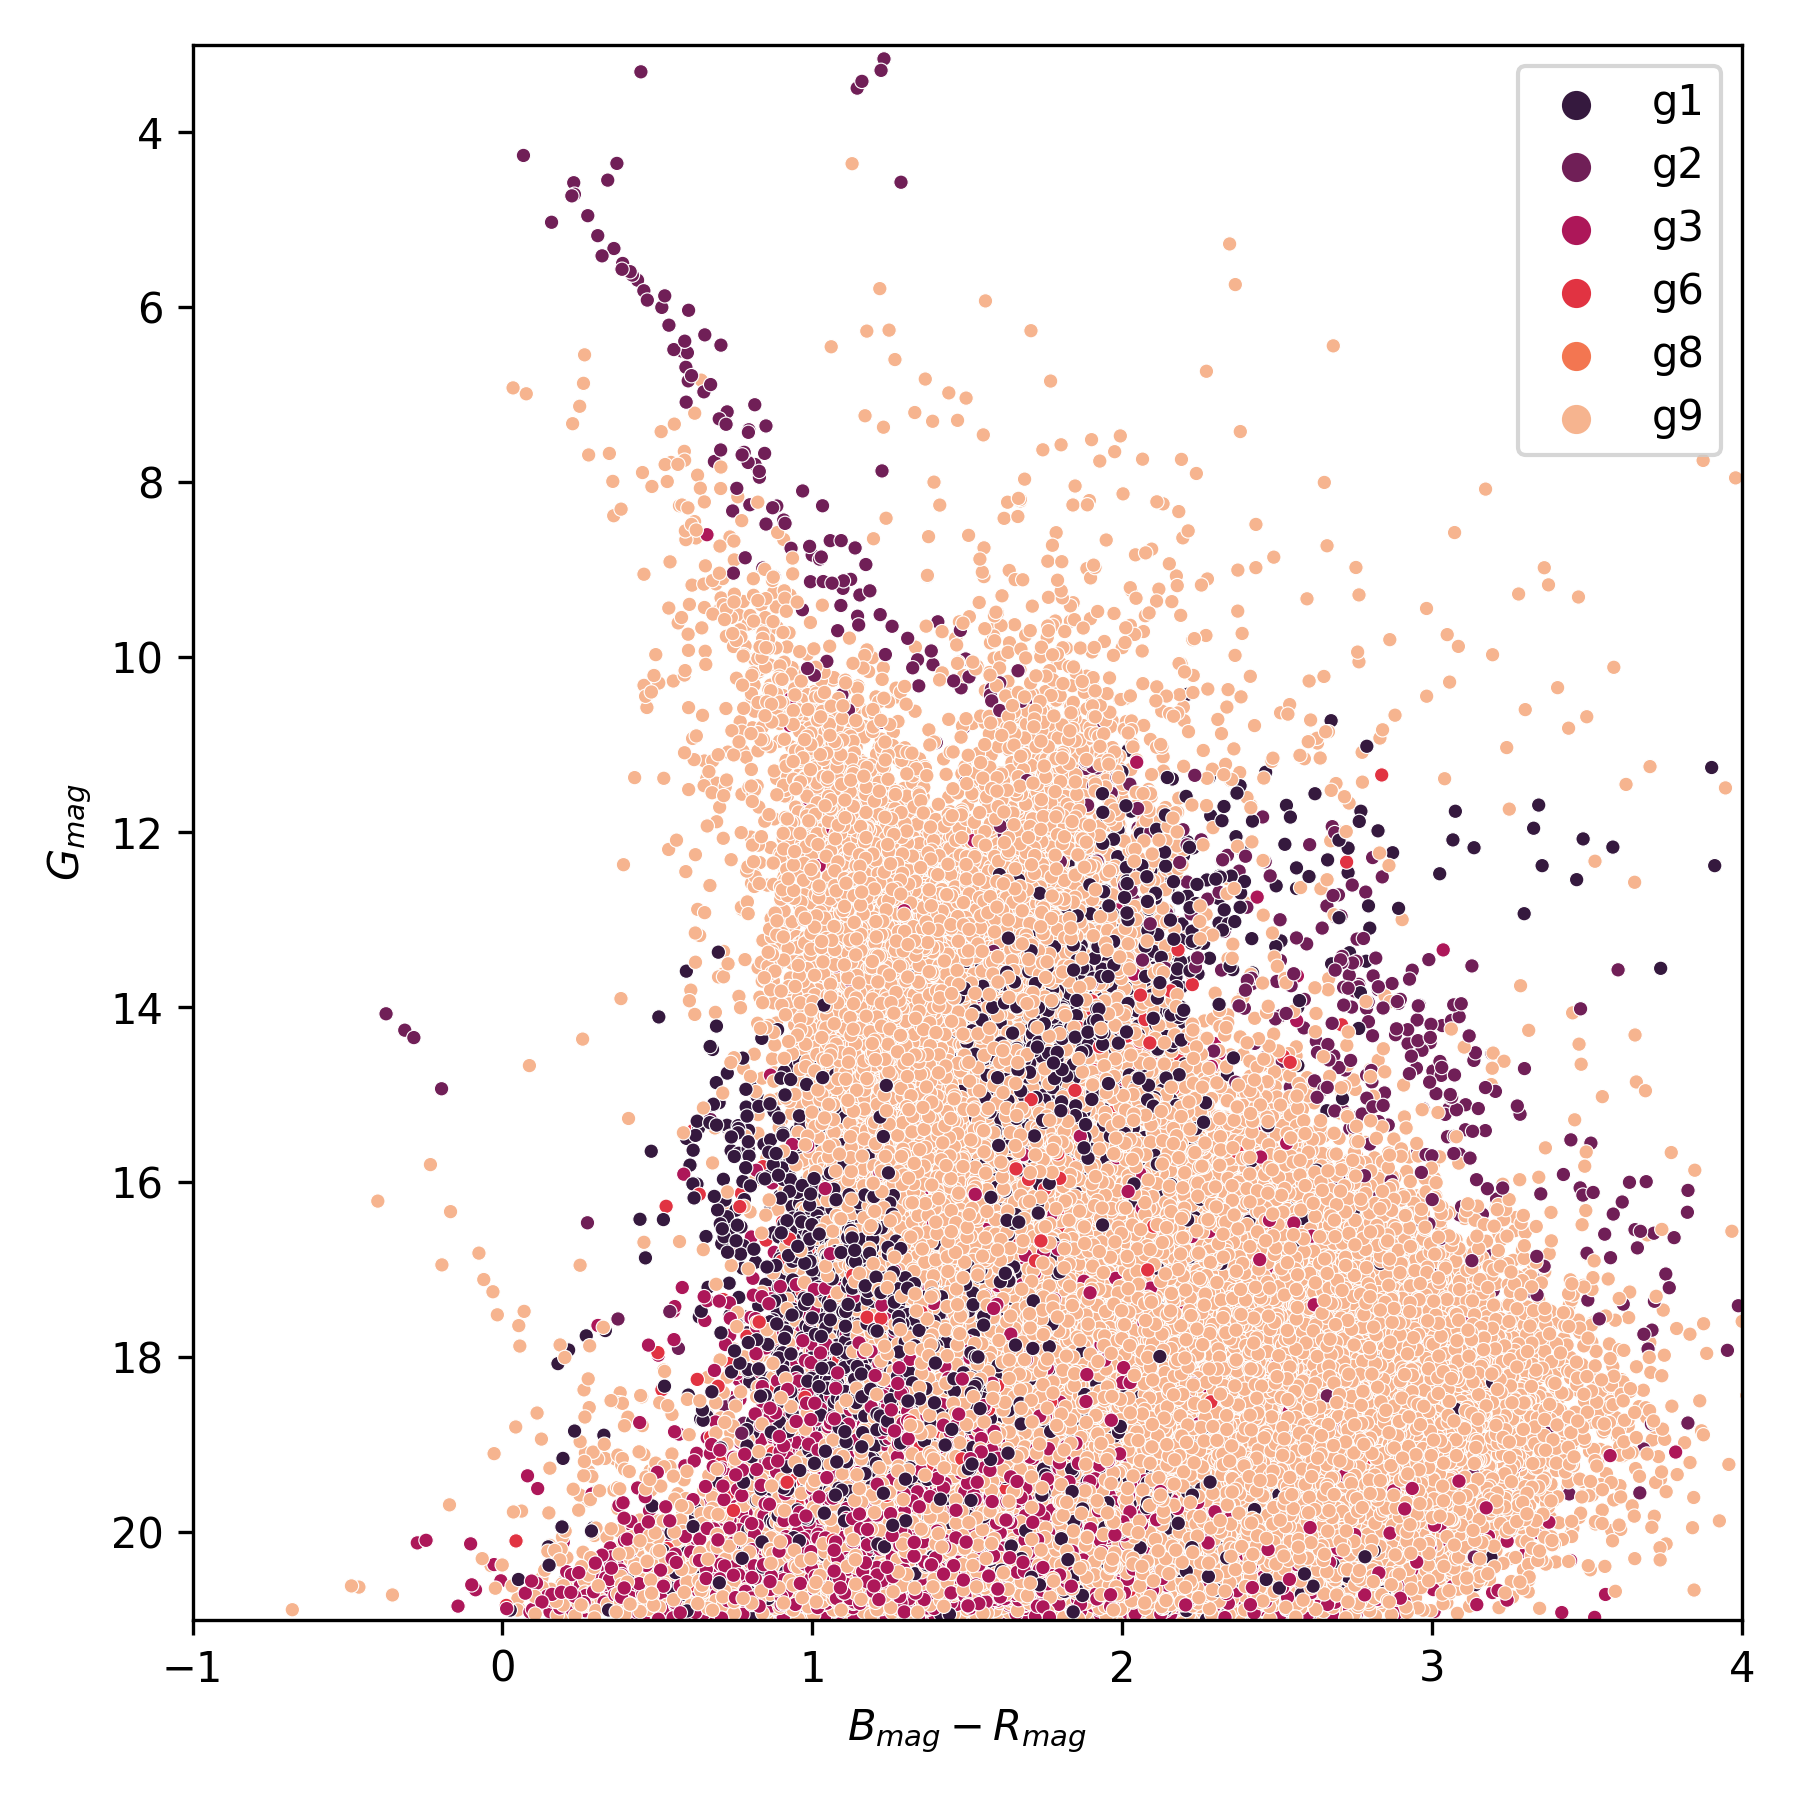
\includegraphics[width=\textwidth]{../figures/melotte_25/dec_hr_diagram_melotte_25.png}
      \caption{DECOCC}
  \end{subfigure}
  \medskip
  \begin{subfigure}[b]{0.3\textwidth}
    \centering
      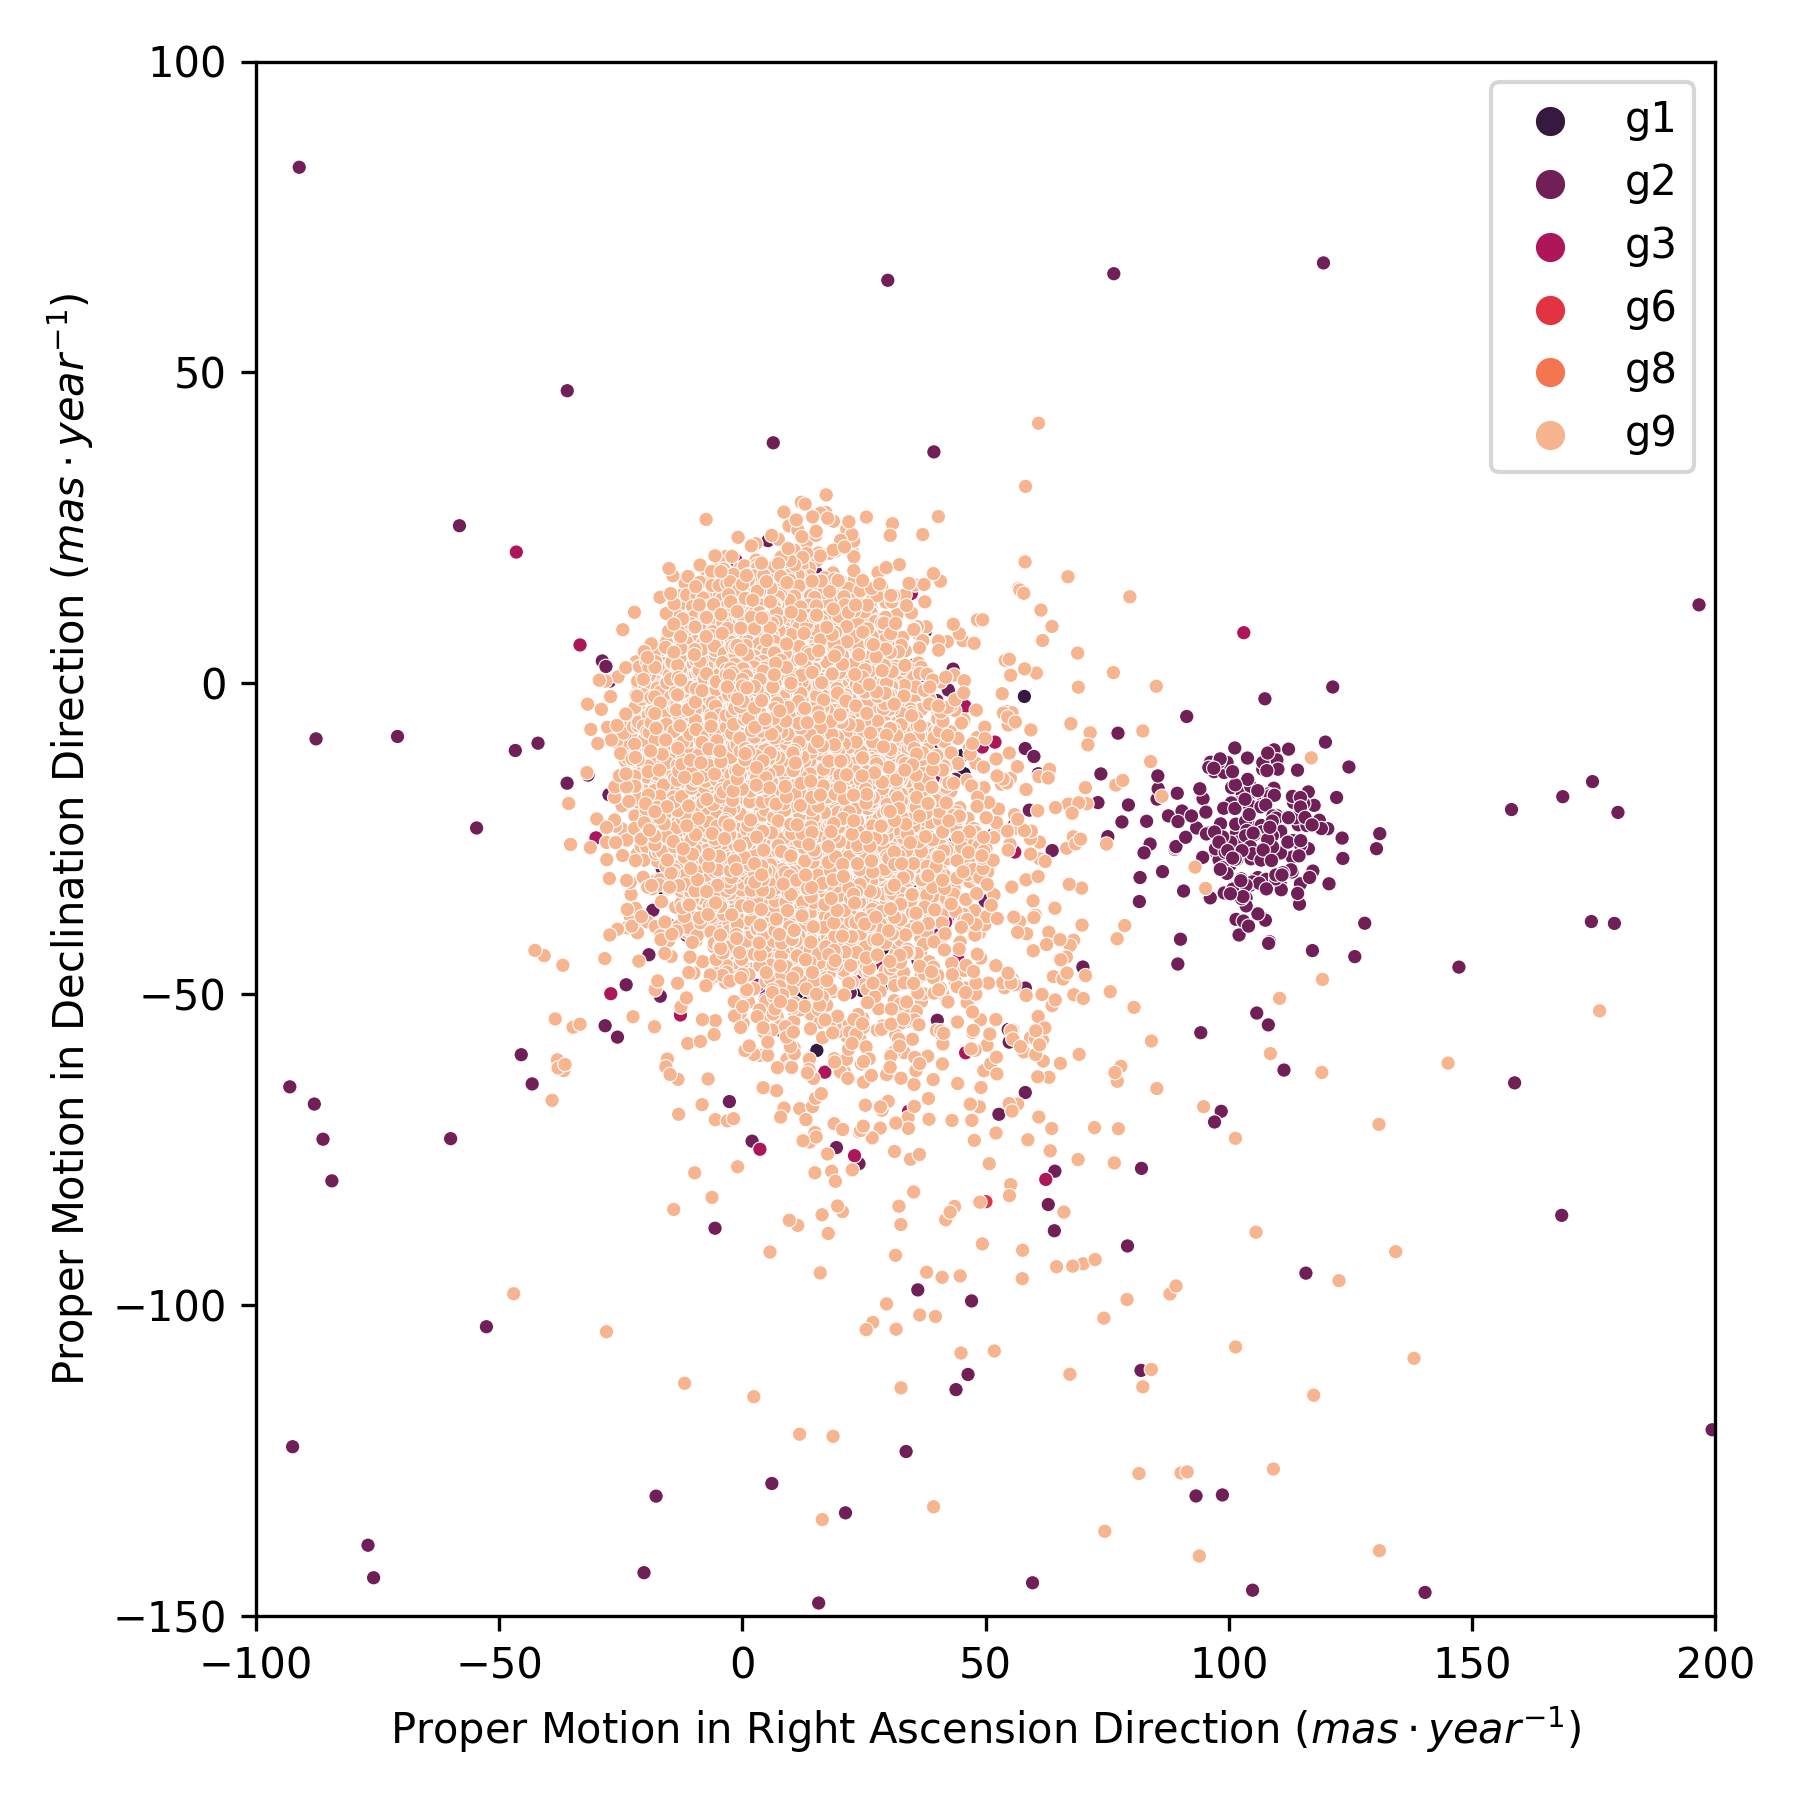
\includegraphics[width=\textwidth]{../figures/melotte_25/dec_pm_filtered_melotte_25.png}
      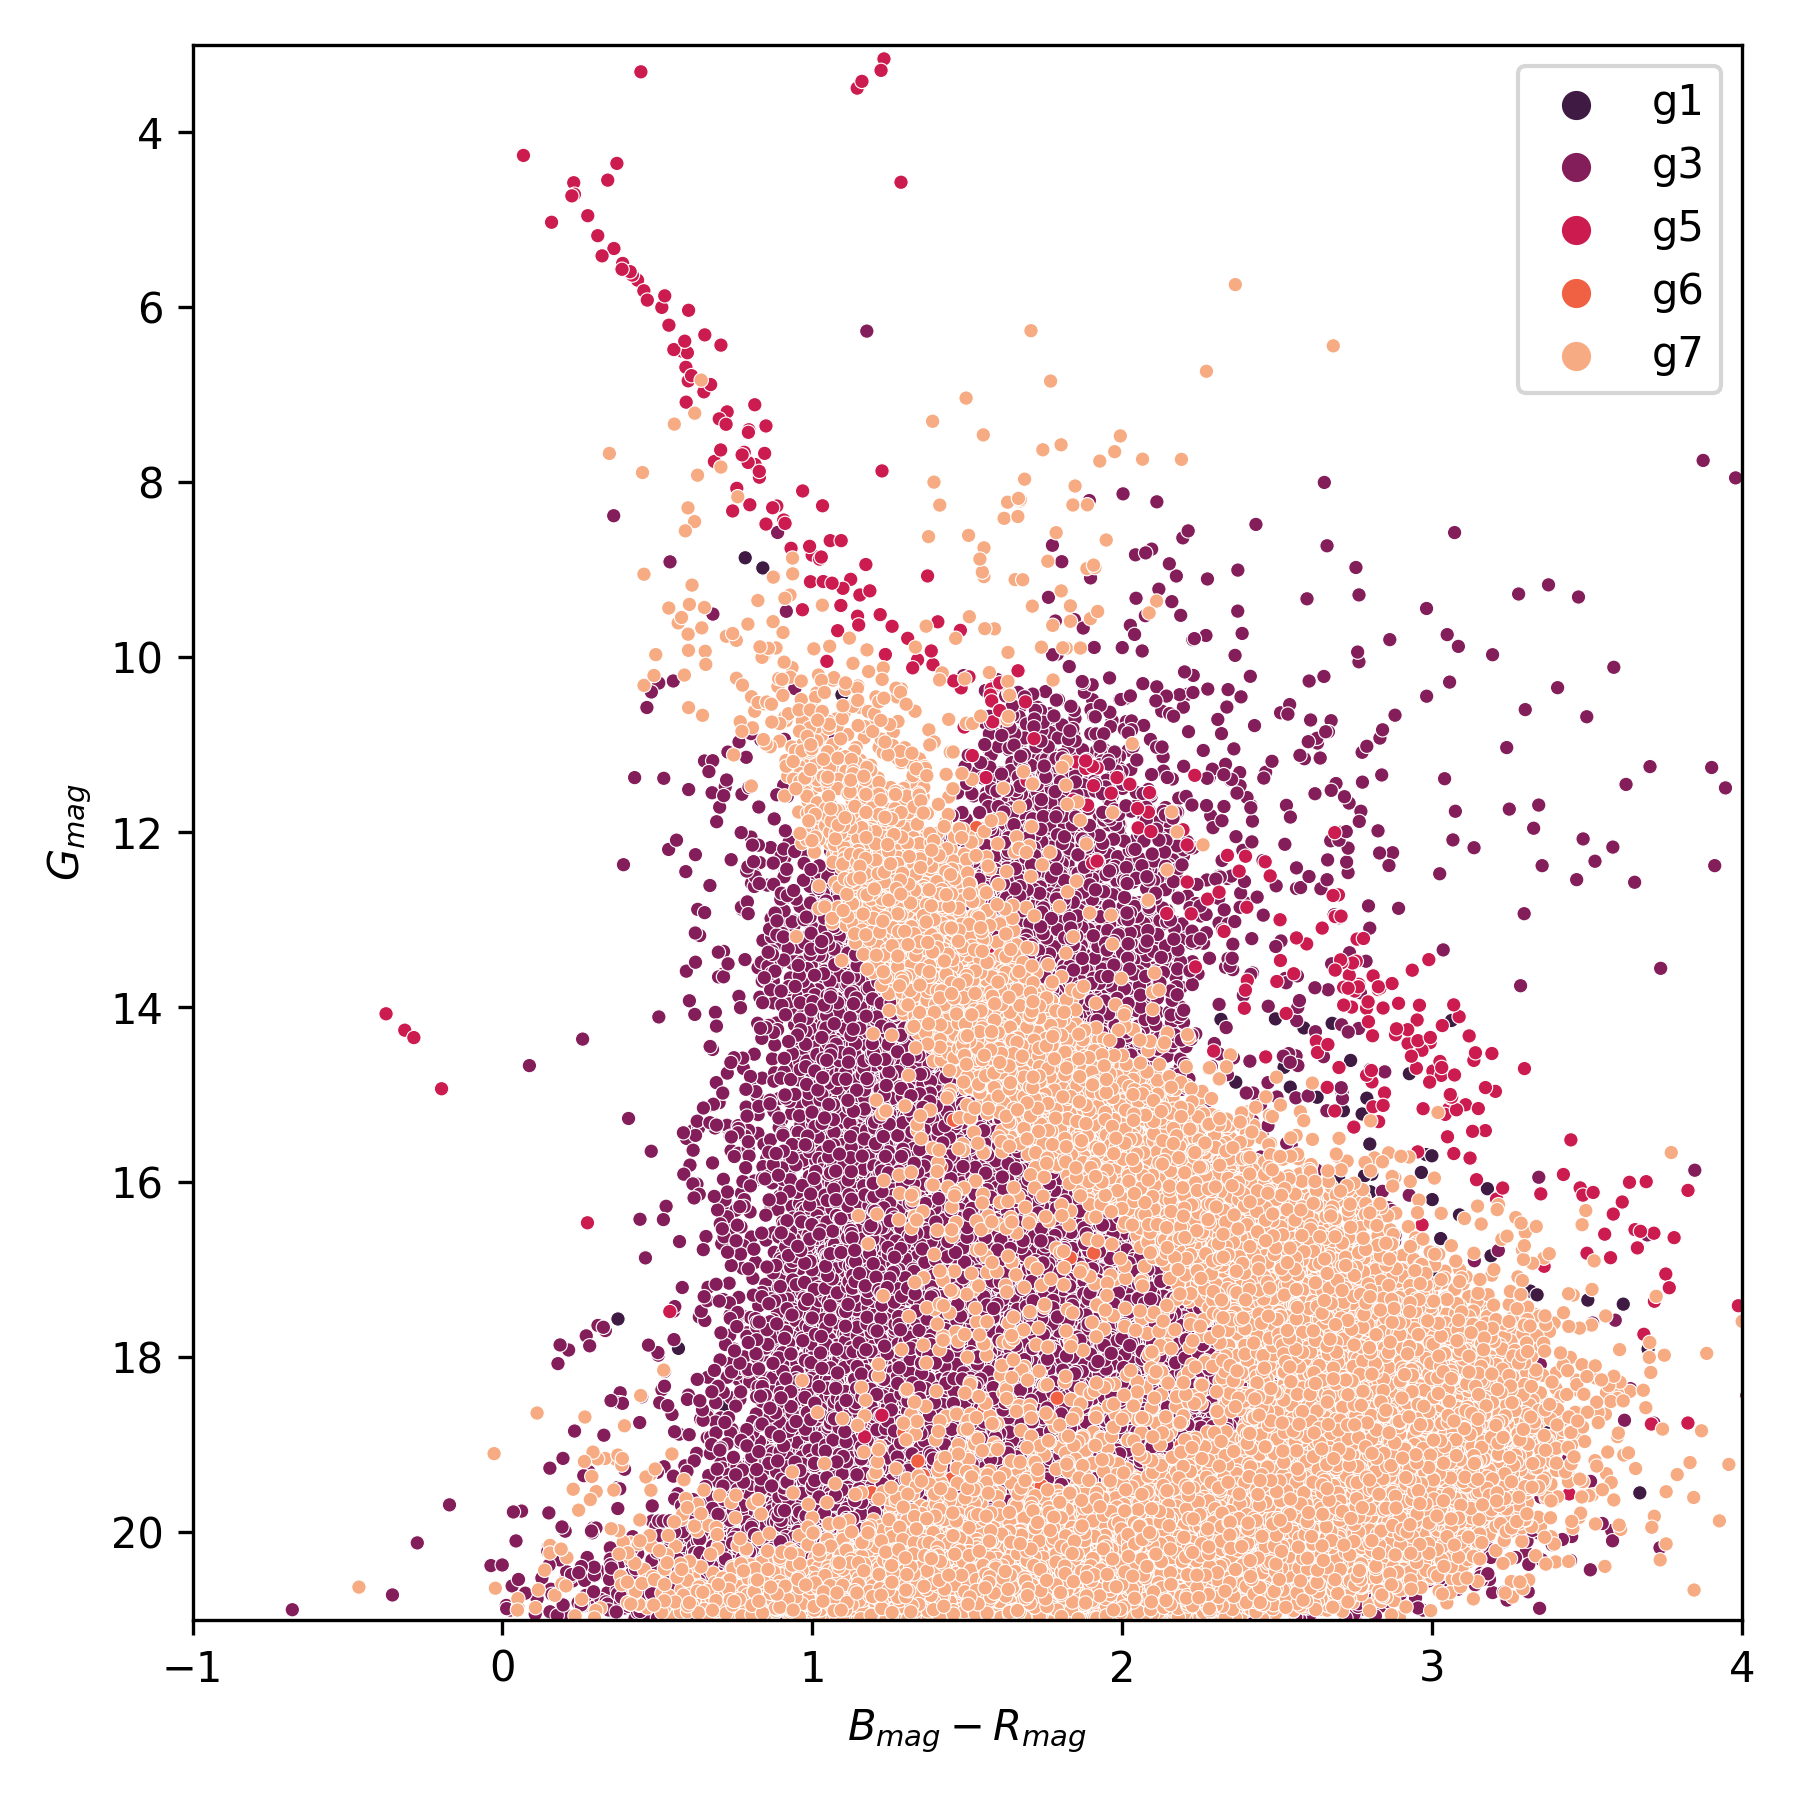
\includegraphics[width=\textwidth]{../figures/melotte_25/dec_hr_diagram_filtered_melotte_25.png}
      \caption{DECOCC (filt.)}
  \end{subfigure}
  \caption{Evolution of Melotte 25 characterization}
  \label{fig:melotte_25_characterization_evolution}
\end{figure*}

Since we are looking for a single cluster, it seems reasonable to use a clustering algorithm like K-Means to find two clusters. One for the desired OC and another for stars that do not belong to the OC. However, the idea is not completely right. This is due to the fact that OC's stars are surrounded by other stars with possibly similar properties. Therefore, setting the number of clusters to two is too low to separate them properly.

Figure~\ref{fig:kmeans_comparisons_melotte_22} shows an example. It describes the results of applying different configurations of K-Means in Melotte 22, N=2, N=5 and N=8. For each configuration of K-Means, we show the proper motion in right ascension and declination (figures in the top position), and the parallax distribution (figures in the down position).

As we can see in the parallax distribution, lower values of the number of clusters (e.g., N=2) assign many stars to the group \emph{g0} (purple) that should belong to group \emph{g1}. These badly assigned stars are the ones that have the parallax far from the 7.3mas resonance. In contrast, large values of the number of clusters allow us to isolate more accurately the resonance in parallax at \(\approx 7.3mas\). For instance, at N=8, more groups are better compartmentalized. Group \emph{g2} would be the one corresponding to the OC that we are looking for, and all the other groups are those that we would like to be a single group. That is the stars that do not belong to the OC. The disadvantage is that K-Means with N=8 forms more groups of stars, which complicates the task of finding the desired OC, since we would like to get just two groups. Therefore, with a K-Means we have to find a way to set the right value for the number of clusters to isolate the searched cluster without creating too many groups. To solve this issue, we can try to estimate the best number of clusters by using the \emph{silhouette score}~\cite{rousseeuw1987silhouettes}.

K-Means does a good job making an initial clustering. However, too many clusters arise from this characterization and the OC is still polluted with stars that do not belong to it. Moreover, we would like to reduce the amount of clusters too.


\section{Results}
\label{sec:results}

We performed two tested of our model:

\begin{enumerate}
  \item with the Melotte 25 dataset, which is one of the most difficult dataset to characterize OC by its distribution and extension, because it is located in a region with 400,000 stars.
  \item with a variety of clusters of different typologies.
\end{enumerate}

In order to support the discussion presented in Section~\ref{sec:deep_open_clustering}, in the both tests we compared our model against a K-Means classification algorithm. In addition, we perform a second execution only in our model where we filtered the quantiles in the Melotte 25 dataset.

Our DECOCC model was implemented in Python 3.8 using the Keras 2.2 framework and Jupyter Notebooks~\cite{Kluyver2016jupyter}. All tests were run on an Apple Mac Pro Late 2013 with a 2.7GHz 12-Core Intel Xeon E5-2697v2, and 64GB RAM 1866MHz DDR3. For the GPU, we use a graphic card AMD FirePro D700 with 6GB~\footnote{All resources developed for this project are available at [LINK]}.
%\href{https://github.com/cdalvaro/machine-learning-master-thesis}{https://github.com/cdalvaro/machine-learning-master-thesis}}.


\subsection{Melotte 25 Dataset}

Figure~\ref{fig:melotte_25_characterization_evolution} shows the evolution of the characterization of Melotte 25. The first column corresponds to the characterization obtained by applying only K-Means (with N=10). The middle column shows the result of our model. And the last column describes the characterization made by our model but filtering the quantiles lower than 0.10 and higher than 0.90. The top row shows the proper motion configuration space, while the bottom one shows the Hertzsprung–Russell diagrams.

%% Comparación con K-Means, DEC y DEC filter

The clustering made by K-Means arises 9 groups, but most of them contain stars that do not belong to the Melotte 25 OC. However, in our model, the stars regroup and although we have the same 9 groups of K-Means, almost all of the stars are assigned to a group that would contain the stars that would not belong to the OC. The remaining groups contain either the OC we are looking for or other possible new OCs inside the studied region. Moreover, if we exclude those stars that remain below 0.10 and above 0.90 percentiles, and execute again this refinement in our model (third column in Figure~\ref{fig:melotte_25_characterization_evolution}), we observe an improvement in the results of our DECOCC model.

\begin{figure}[!hbt]
  % \centering
  % \begin{subfigure}[t]{0.30\textwidth}
  %   \centering
  %   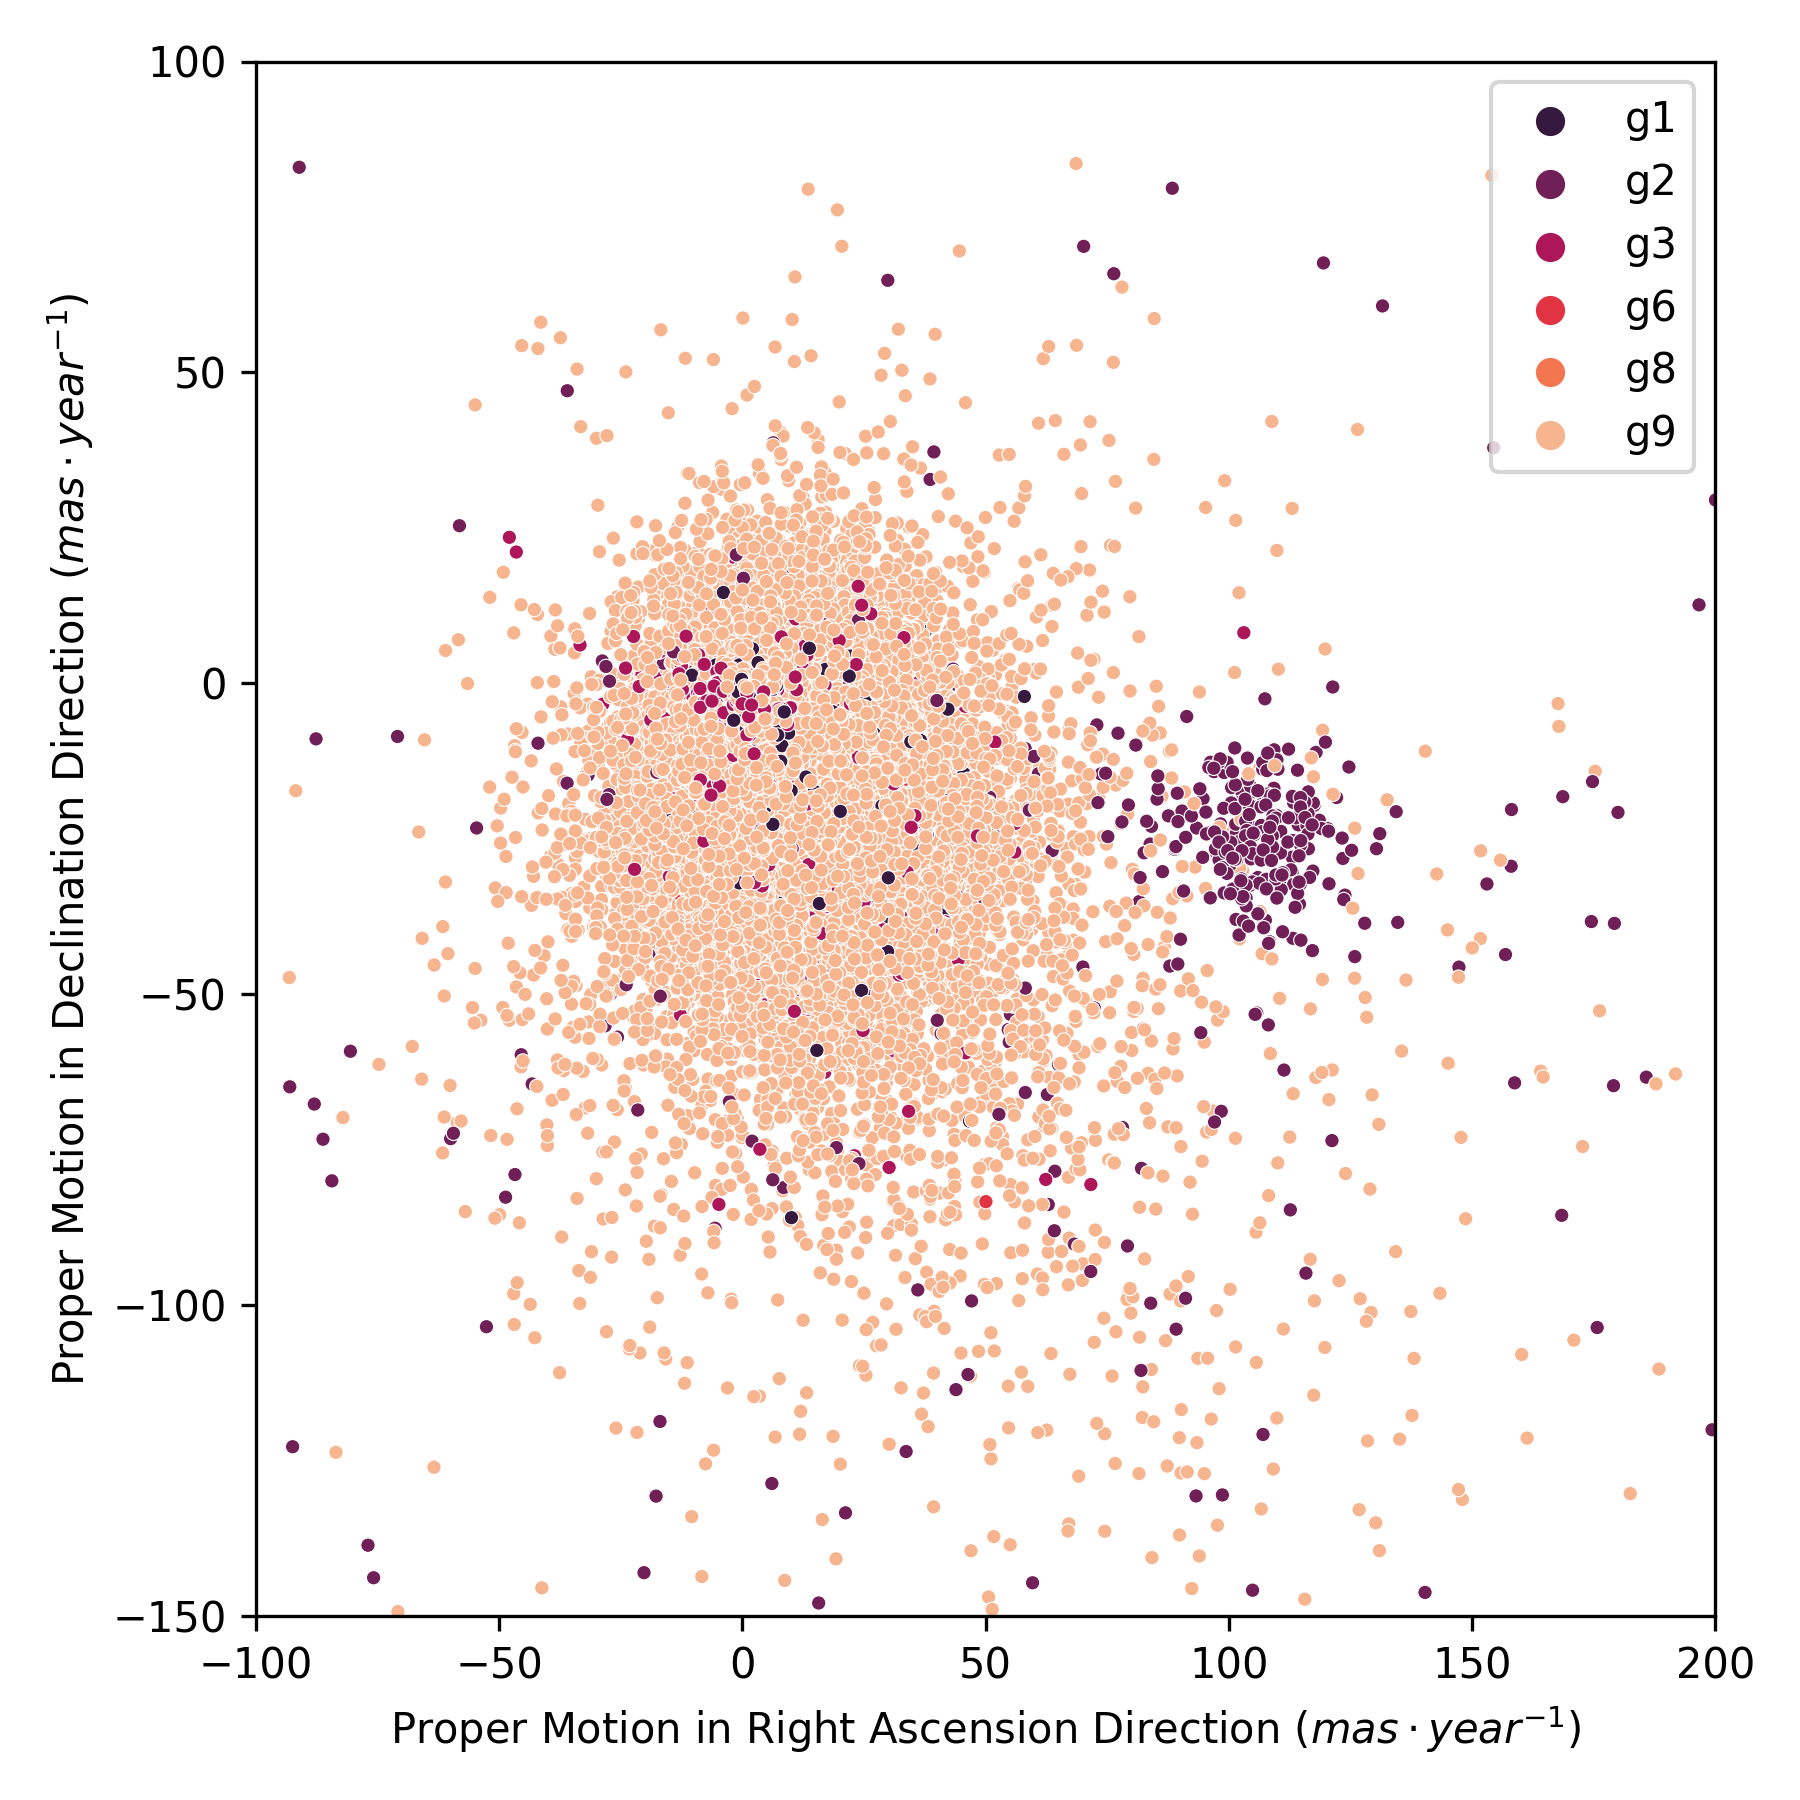
\includegraphics[width=\textwidth]{../figures/melotte_25/dec_pm_melotte_25.png}
  % \end{subfigure}
  % \hfill
  % \begin{subfigure}[t]{0.30\textwidth}
    \centering
    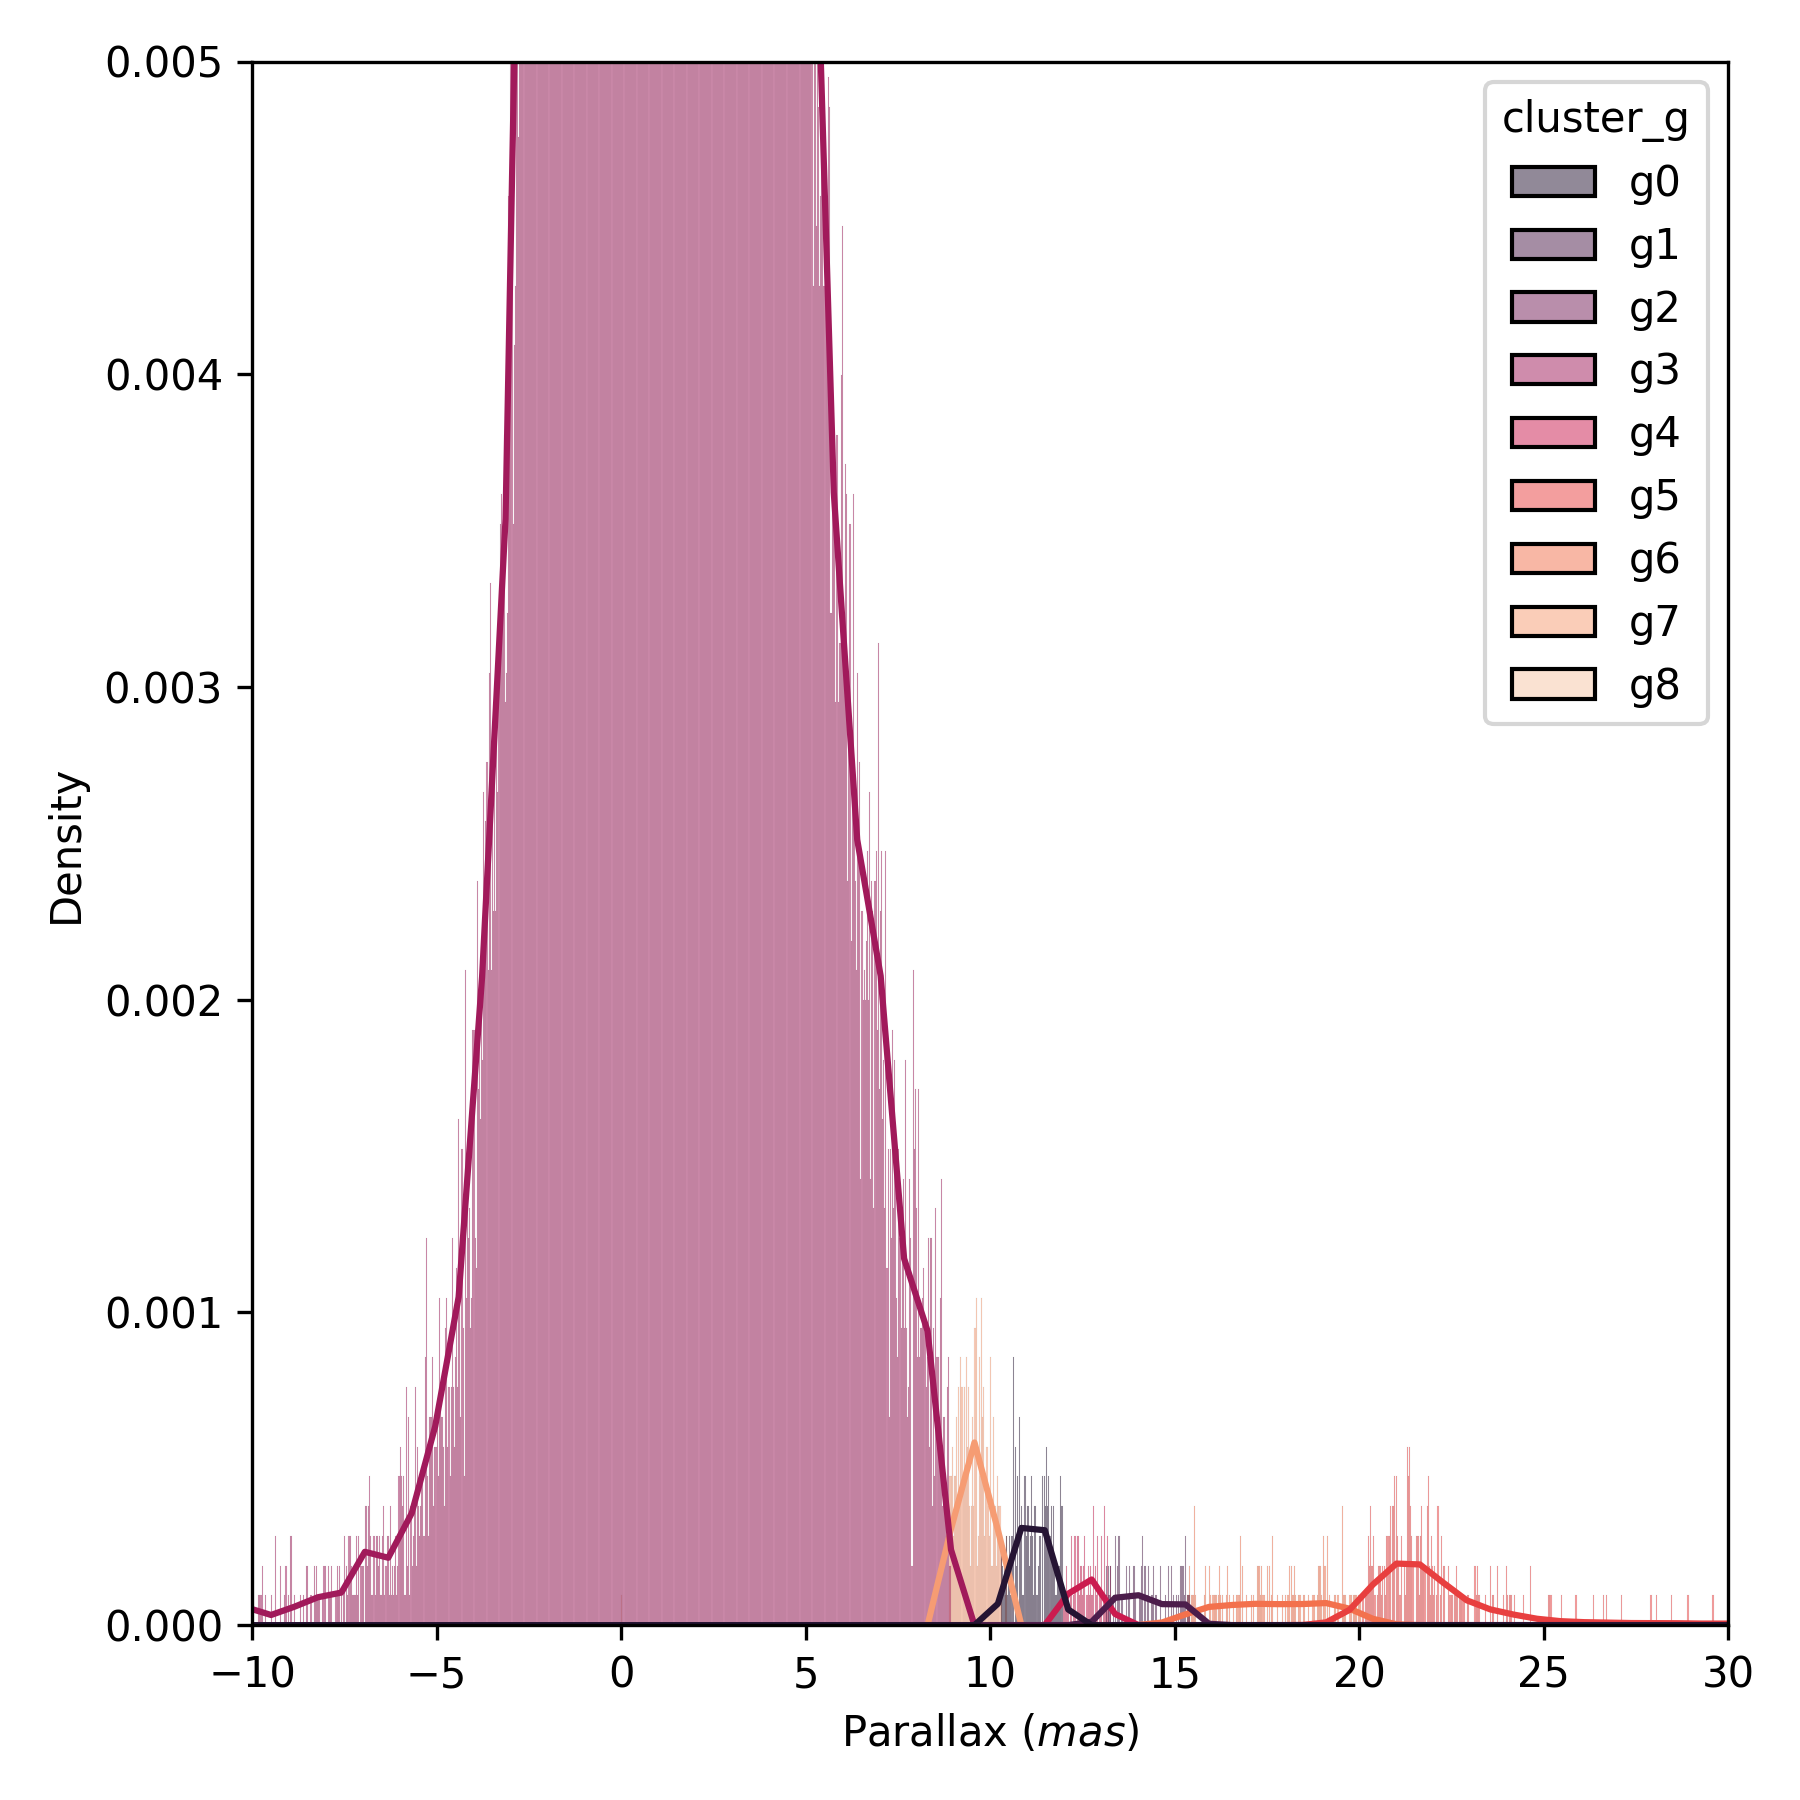
\includegraphics[width=0.36\textwidth]{../figures/melotte_25/dec_parallax_melotte_25.png}
  % \end{subfigure}
  % \hfill
  % \begin{subfigure}[t]{0.30\textwidth}
  %   \centering
  %   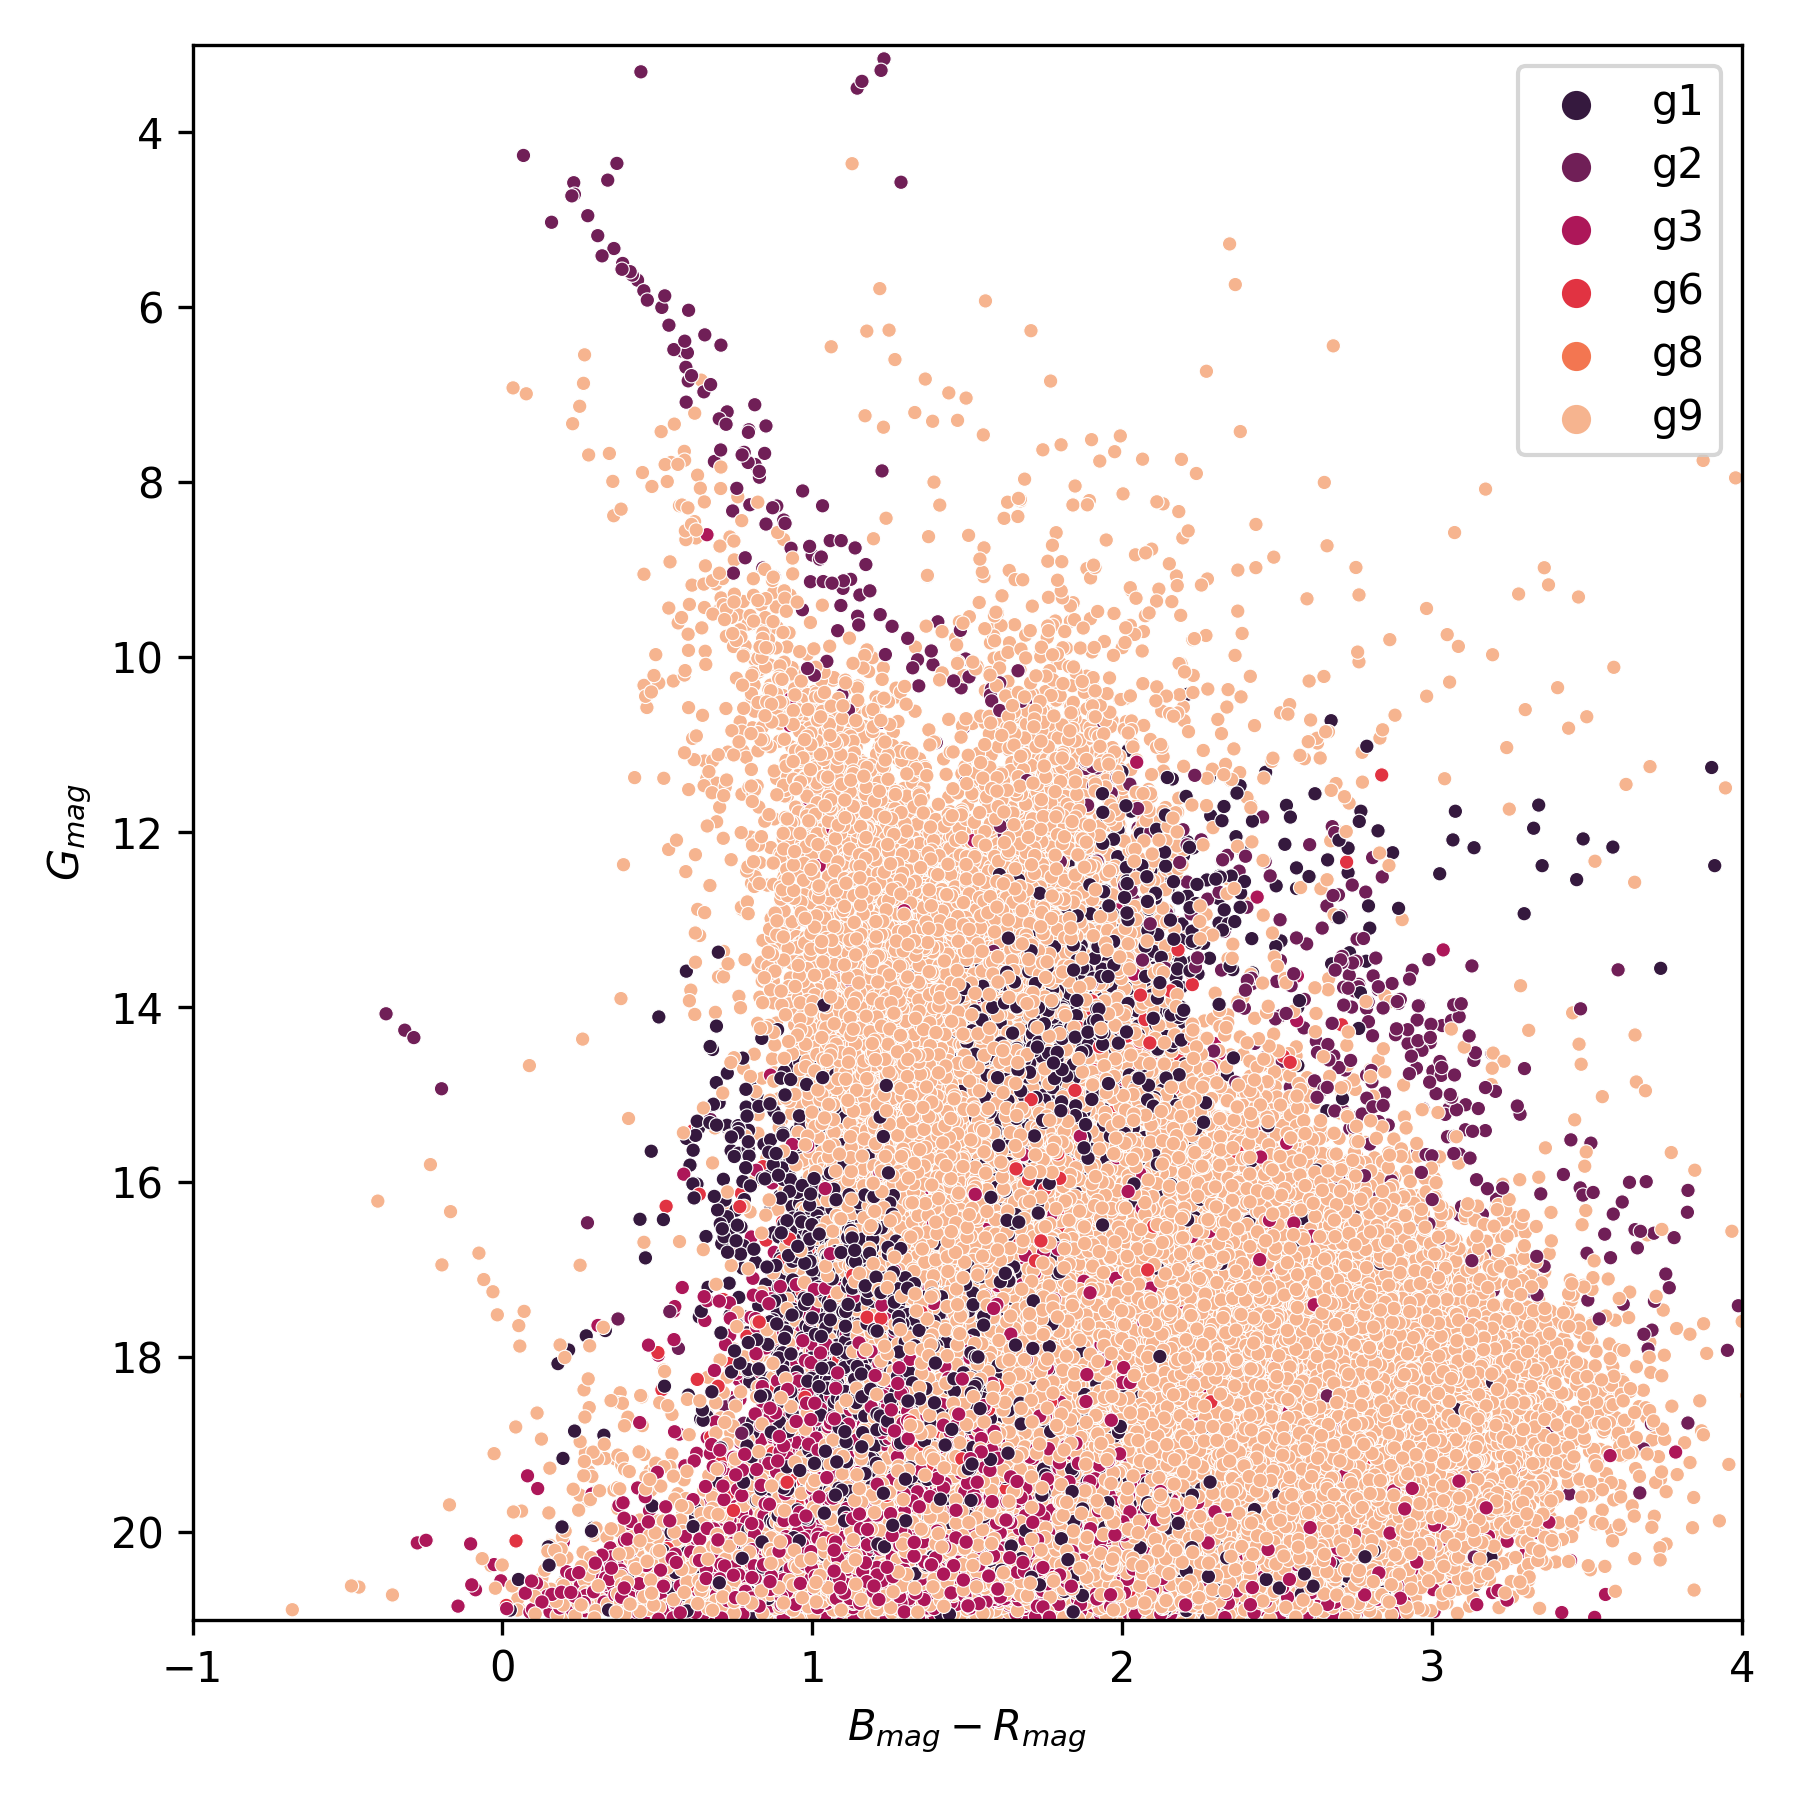
\includegraphics[width=\textwidth]{../figures/melotte_25/dec_hr_diagram_melotte_25.png}
  % \end{subfigure}
  % \caption{Melotte 25 characterization. From left to right: proper motion configuration space, parallax histogram and H-R diagram.}
  \caption{Parallax histogram of Melotte 25 characterization.}
  \label{fig:result_melotte_25_dec}
\end{figure}

The dataset Melotte 25 is located at 66.725 degrees in right ascension and 15.867 degrees in declination with a radius of 165 arcmin. As it was mentioned before, this region contains more than 400,000 stars making it difficult to group stars of the same region. Our model labels Melotte 25 as group \emph{g5}. Figure~\ref{fig:result_melotte_25_dec} shows the parallax histogram.

\begin{table}[!htbp]
  \begin{center}
    \resizebox{\columnwidth}{!}{
      \begin{tabular}{l|c|c|c|c}
        \textbf{Method} & \emph{\(\mu_{\alpha}\) \((mas \cdot yr^{-1})\)} & \emph{\(\mu_{\delta}\) \((mas \cdot yr^{-1})\)}
        & \emph{\( \varpi \) \((mas)\)} & \emph{\# stars} \\
        \hline
        Simbad & 104.92 \( \pm \) 0.12 & -28.00 \( \pm \) 0.09 & 21.052 \( \pm \) 0.065 & - \\
        % Clusterix & 106.796 \( \pm \) 6.229 & -24.870 \( \pm \) 5.417 & 21.210 \( \pm \) 1.115 & 109 \\
        K-Means & 79.936 \( \pm \) 3.7 & -45.362 \( \pm \) 3.8 & 20.901 \( \pm \) 0.31 & 374 \\
        DECOCC & 104.051 \( \pm \) 3.2 & -33.424 \( \pm \) 2.5 & 22.072 \( \pm \) 0.13 & 219 \\
        DECOCC (filt.) & 105.96 \( \pm \) 3.5 & -30.00 \( \pm \) 2.4 & 21.74 \( \pm \) 0.07 & 175 \\
      \end{tabular}
    }
    \caption{Summary for the Melotte 25 results.}
    \label{tab:results_melotte_25}
  \end{center}
\end{table}

Table~\ref{tab:results_melotte_25} summarizes the results for the Melotte 25 dataset. The first column shows the name of the method. Second and third columns describe the proper motion in right ascension and declination, respectively. The fourth column shows the parallax. And the last column presents the number of stars corresponding to the OC. Columns from second to fourth have their respective deviations computed as the standard error of the predicted group.

By comparing the results obtained with our DECOCC model, we can see that they are in range with those extracted from Simbad astronomical database~\cite{wenger2000simbad} (first row in Table~\ref{tab:results_melotte_25}). While the results provided by K-Means model are far from the official data. This comparison demonstrates that our model improves the results obtained with a raw K-Means.

\begin{table}[!htb]
  \begin{center}
    \begin{tabular}{l|c}
      \textbf{Hyperparameter} & \textbf{Value} \\
      \hline
      Number of Clusters & 9 \\
      Clustering Layer & \(\left[ 50, 50, 40 \right]\) \\
      Kernel Initializer Seed & 11 \\
      Quantil Threshold & 0.1 \\
    \end{tabular}
    \caption{Hyperparameters for Melotte 25.}
    \label{tab:hyperparameters_melotte_25}
  \end{center}
\end{table}

Table~\ref{tab:hyperparameters_melotte_25} shows the hyperparameters used for the characterization. We used them to fine-tuning our model and improve its accuracy. Although they depend on the studied region, none of them are related with physical properties of the cluster, which makes it easy to automate the selection of hyperparameters.

\subsection{Clusters With Different Typologies}

We perform now more exhaustive tests of our DECOCC model using open clusters with different typologies (e.g., large, small, more extensive, or more concentrated within the region to be analyzed):

\begin{itemize}
  \item NGC 2516, which has the proper motion center deviated from the origin but embedded within a large cloud of stars with similar proper motions.
  \item NGC 2632, which, in addition to Melotte 22 (explained below), is a cluster whose proper motion center is not at the origin and has a well-separated parallax center.
  \item NGC 2682, which has the parallax centered within the region's Gaussian, making it difficult its detection. Moreover, same as NGC 2516, the proper motion center is deviated from the origin.
  \item Melotte 22, as well as Melotte 25, is a cluster closer to our galaxy. That causes its membership stars to be more scattered than previous clusters which are more compact.
\end{itemize}

Table~\ref{tab:clusters_summary} describes more specific information about the previous clusters (we also include information about the Melotte 25 open cluster, which was previously analyzed). The first column shows the name of the cluster. The remaining columns are the right ascension, declination, radius, and the number of stars of studied clusters. The last column (\# stars) corresponds to those stars contained within a cone of center \((\alpha, \delta)\) and radius the cluster's radius multiplied by a factor of 1.5.

\begin{table}[htbp]
  \begin{center}
    \resizebox{\columnwidth}{!}{
      \begin{tabular}{l|c|c|c|c}
        \textbf{OC} & \emph{\( \alpha \) J2000 \((degrees)\)} & \emph{\( \delta \) J2000 \((degrees)\)}
        & \emph{Radius \((arcmin)\)} & \emph{\# stars} \\
        \hline
        NGC 2516 & 119.517 & -60.753 & 15 & 12,869 \\
        NGC 2632 & 130.1 & 19.667 & 35 & 13,167 \\
        NGC 2682 & 132.825 & 11.8 & 12.5 & 2,839 \\
        Melotte 22 & 56.75 & 24.117 & 60 & 61,552 \\
        Melotte 25 & 66.725 & 15.867 & 165 & 433,996 \\
      \end{tabular}
    }
    \caption{Properties of clusters for further testing of our model.}
    \label{tab:clusters_summary}
  \end{center}
\end{table}

%% Tabla comparativa de todos los open clusters
\begin{table*}[!htb]
  \begin{center}
    % \resizebox{\columnwidth}{!}{
      \begin{tabular}{c|l|c|c|c|c}
         & Method & \emph{\(\mu_{\alpha}\) \((mas \cdot yr^{-1})\)} & \emph{\(\mu_{\delta}\) \((mas \cdot yr^{-1})\)}
        & \emph{\( \varpi \) \((mas)\)} & \emph{\# stars} \\
        \hline
        \multirow{4}{*}{\rotatebox[origin=c]{90}{NGC 2516}}
        & Simbad & -4.6579 \( \pm \) 0.0075 & 11.1517 \( \pm \) 0.0075 & 2.4118 \( \pm \) 0.0006 & 1727 \\
        & K-Means & -4.344 \( \pm \) 0.14 & 9.507 \( \pm \) 0.19 & 2.268 \( \pm \) 0.01 & 1542 \\
        & DECOCC & -4.426 \( \pm \) 0.17 & 9.952 \( \pm \) 0.20 & 2.436 \( \pm \) 0.01 & 1532 \\
        & DECOCC (filt.) & -4.502 \( \pm \) 0.14 & 10.114 \( \pm \) 0.17 & 2.392 \( \pm \) 0.004 & 1072 \\\\

        % \caption{NGC 2632 results.}
        \multirow{4}{*}{\rotatebox[origin=c]{90}{NGC 2632}} & Simbad & -36.047 \( \pm \) 0.110 & -12.917 \( \pm \) 0.066 & 5.371 \( \pm \) 0.003 & - \\
        & K-Means & -26.352 \( \pm \) 0.82 & -15.828 \( \pm \) 0.76 & 5.394 \( \pm \) 0.03 & 629 \\
        & DECOCC & -20.012 \( \pm \) 0.69 & -14.742 \( \pm \) 0.58 & 4.686 \( \pm \) 0.03 & 894 \\
        & DECOCC (filt.) & -21.571 \( \pm \) 0.74 & -14.234 \( \pm \) 0.61 & 4.719 \( \pm \) 0.03 & 714 \\\\

        % \caption{NGC 2682 results.}
         \multirow{4}{*}{\rotatebox[origin=c]{90}{NGC 2682}} & Simbad & -10.9737 \( \pm \) 0.0064 & -2.9396 \( \pm \) 0.0063 & 1.1325 \( \pm \) 0.0011 & 1194 \\
        & K-Means & -8.616 \( \pm \) 0.15 & -3.710 \( \pm \) 0.16 & 1.196 \( \pm \) 0.01 & 1374 \\
        & DECOCC & -8.926 \( \pm \) 0.15 & -3.550 \( \pm \) 0.15 & 1.144 \( \pm \) 0.005 & 1238 \\
        & DECOCC (filt.) & -9.619 \( \pm \) 0.13 & -3.317 \( \pm \) 0.13 & 1.140 \( \pm \) 0.003 & 990 \\\\

        % \caption{Melotte 22 results.}
        \multirow{4}{*}{\rotatebox[origin=c]{90}{Melotte 22}} & Simbad & 19.997 \( \pm \) 0.127 & -45.548 \( \pm \) 0.101 & 7.364 \( \pm \) 0.005 & 1326 \\
        & K-Means & 20.25 \( \pm \) 0.95 & -38.01 \( \pm \) 1.08 & 7.23 \( \pm \) 0.06 & 1378 \\
        & DECOCC & 23.67 \( \pm \) 1.29 & -46.23 \( \pm \) 1.50 & 8.04 \( \pm \) 0.09 & 878 \\
        & DECOCC (filt.) & 19.50 \( \pm \) 0.41 & -44.23 \( \pm \) 0.39 & 7.42 \( \pm \) 0.005 & 438 \\

      \end{tabular}
    % }
    \caption{Summary of the results for the clusters with different typologies.}
    \label{tab:app_results_ngc_2516}
  \end{center}
\end{table*}

As we can see, all those clusters have a wide variety of diameters, from 25 to 330 arcmin, as well as the number of stars that belong to them. For instance, NGC 2682 has 3,000 stars while Melotte 25 is inside a region with more than 400,000 stars.

Table~\ref{tab:app_results_ngc_2516} describes a summary of the results for the clusters with different typologies. Again, our DECOCC model presents similar results from those extracted from the astronomical database Simbad. Except for the open cluster NGC 2632. This is so because the center of the proper motion is not at the origin and generates a more separate center of parallax, which makes it difficult to characterize the open cluster. Compared to K-Means, our model presents more robust results in more difficult open clusters, such as the NGC 2682 that has the parallax centered within the region's Gaussian.

%% comparativa de las figuras de los open clusters
\begin{figure*}[!hbt]
  \rotatebox[origin=c]{90}{{\bfseries NGC 2516}\strut}
  \rotatebox[origin=c]{90}{parallax \strut}
  \begin{subfigure}{0.29\textwidth}
    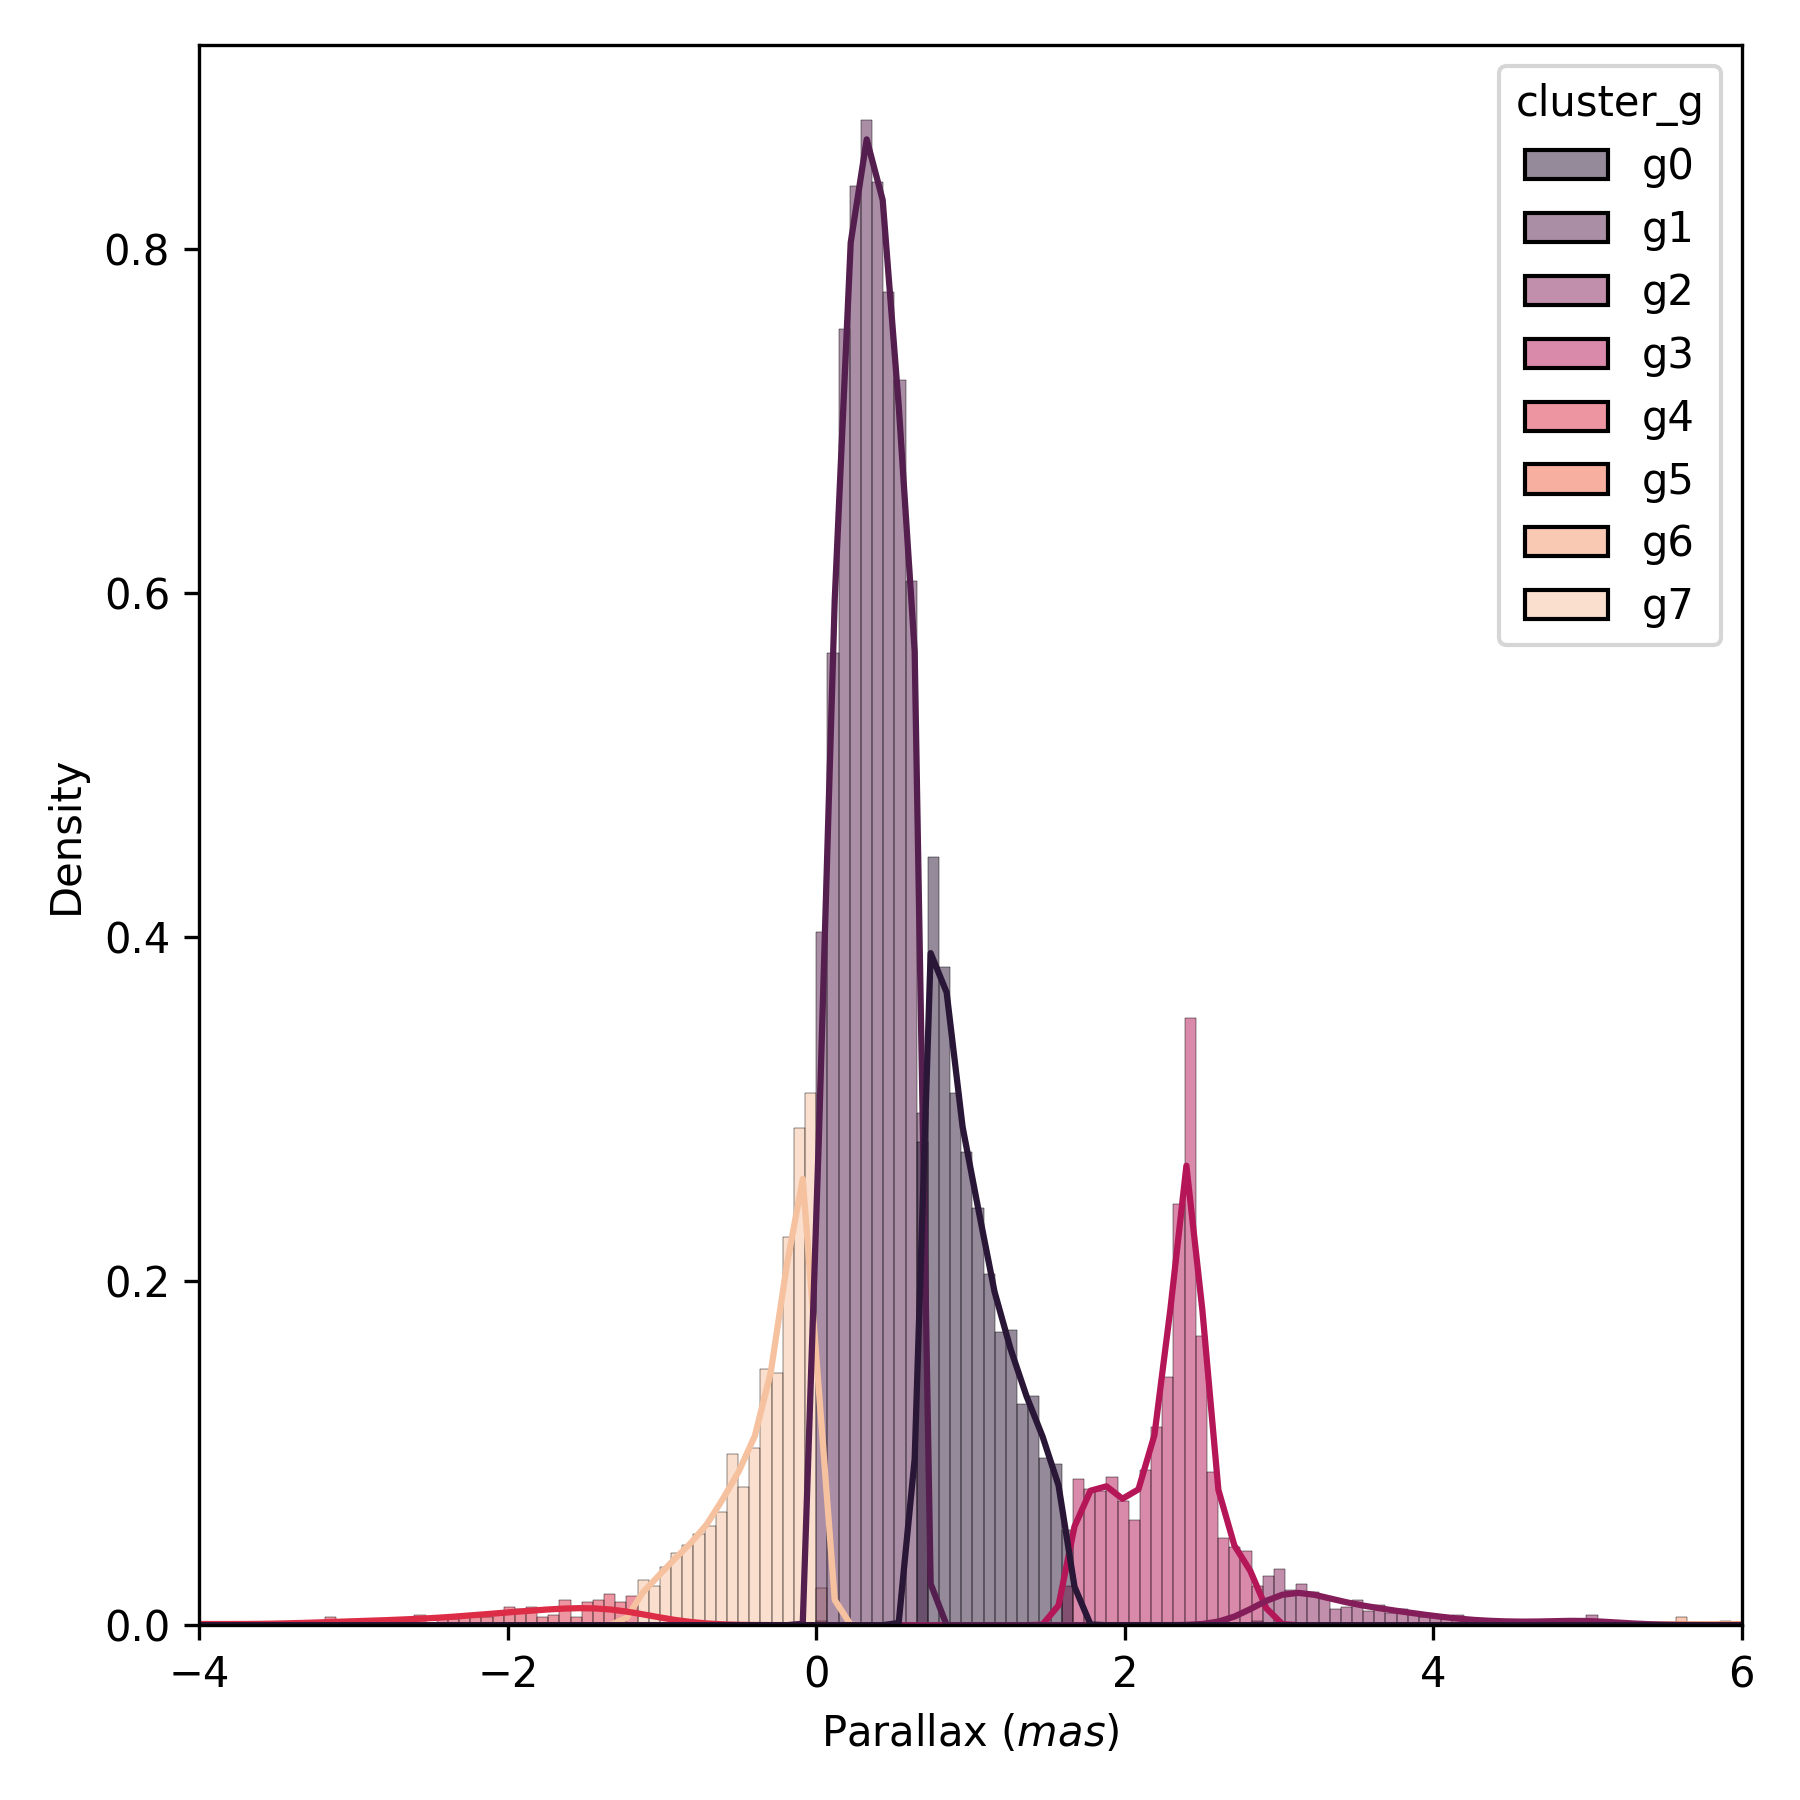
\includegraphics[width=\textwidth]{../figures/ngc_2516/kmeans_parallax_ngc_2516.png}
  \end{subfigure}
  \begin{subfigure}{0.29\textwidth}
    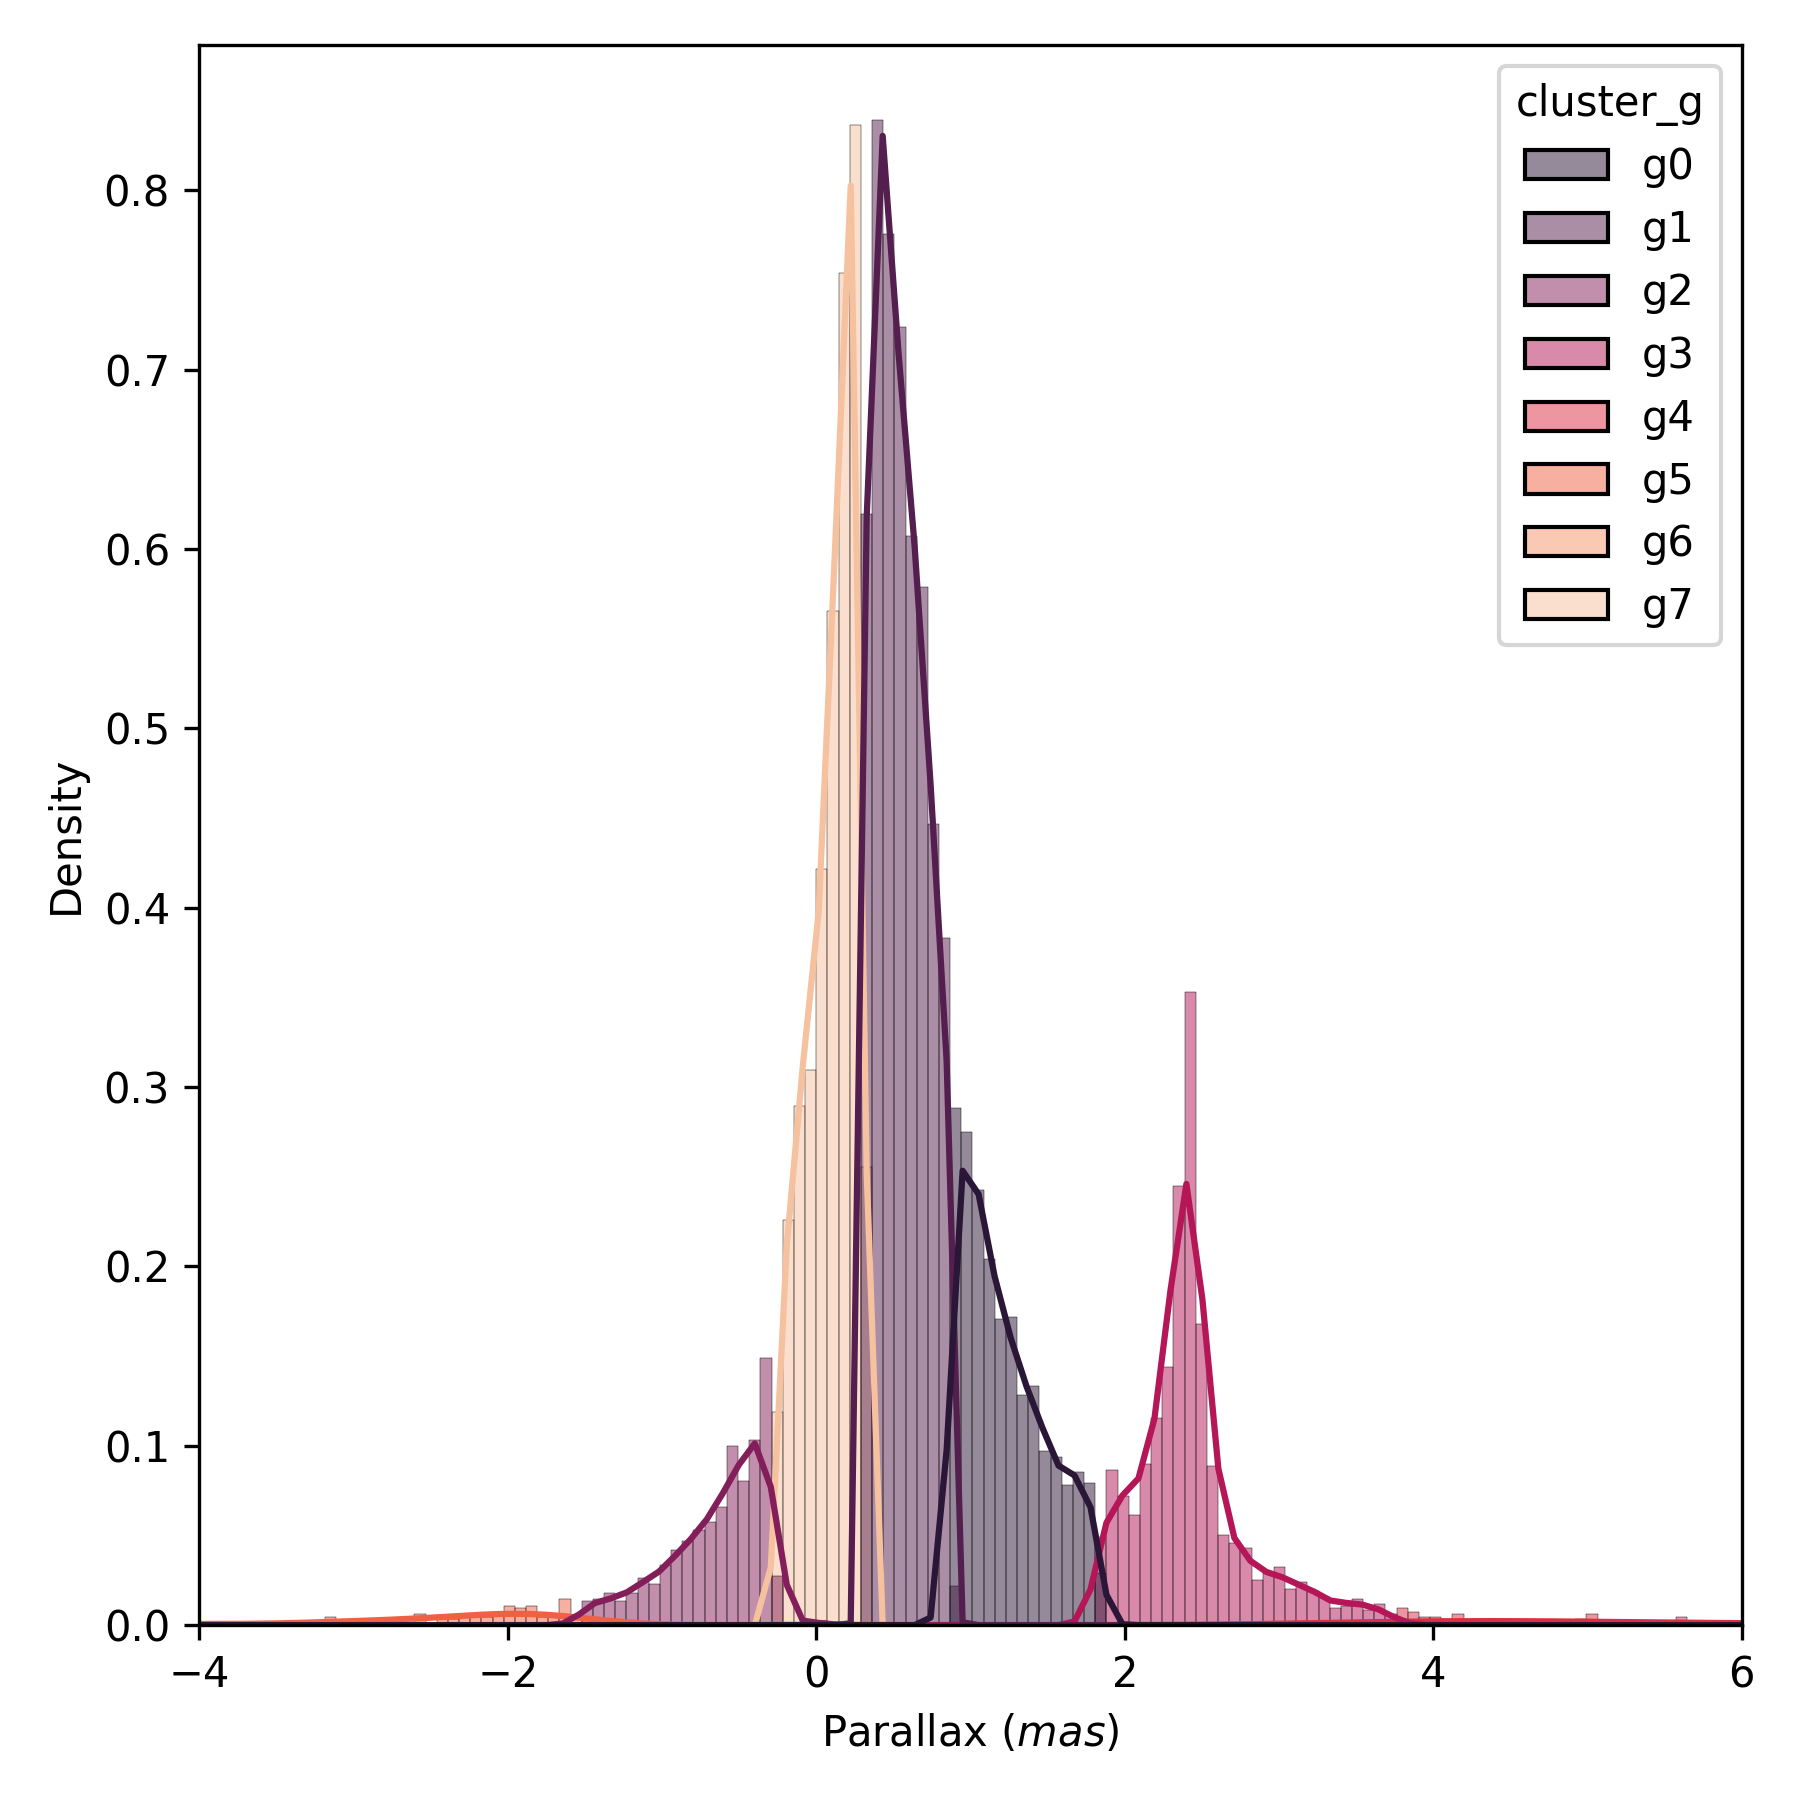
\includegraphics[width=\textwidth]{../figures/ngc_2516/dec_parallax_ngc_2516.png}
  \end{subfigure}
  \begin{subfigure}{0.29\textwidth}
    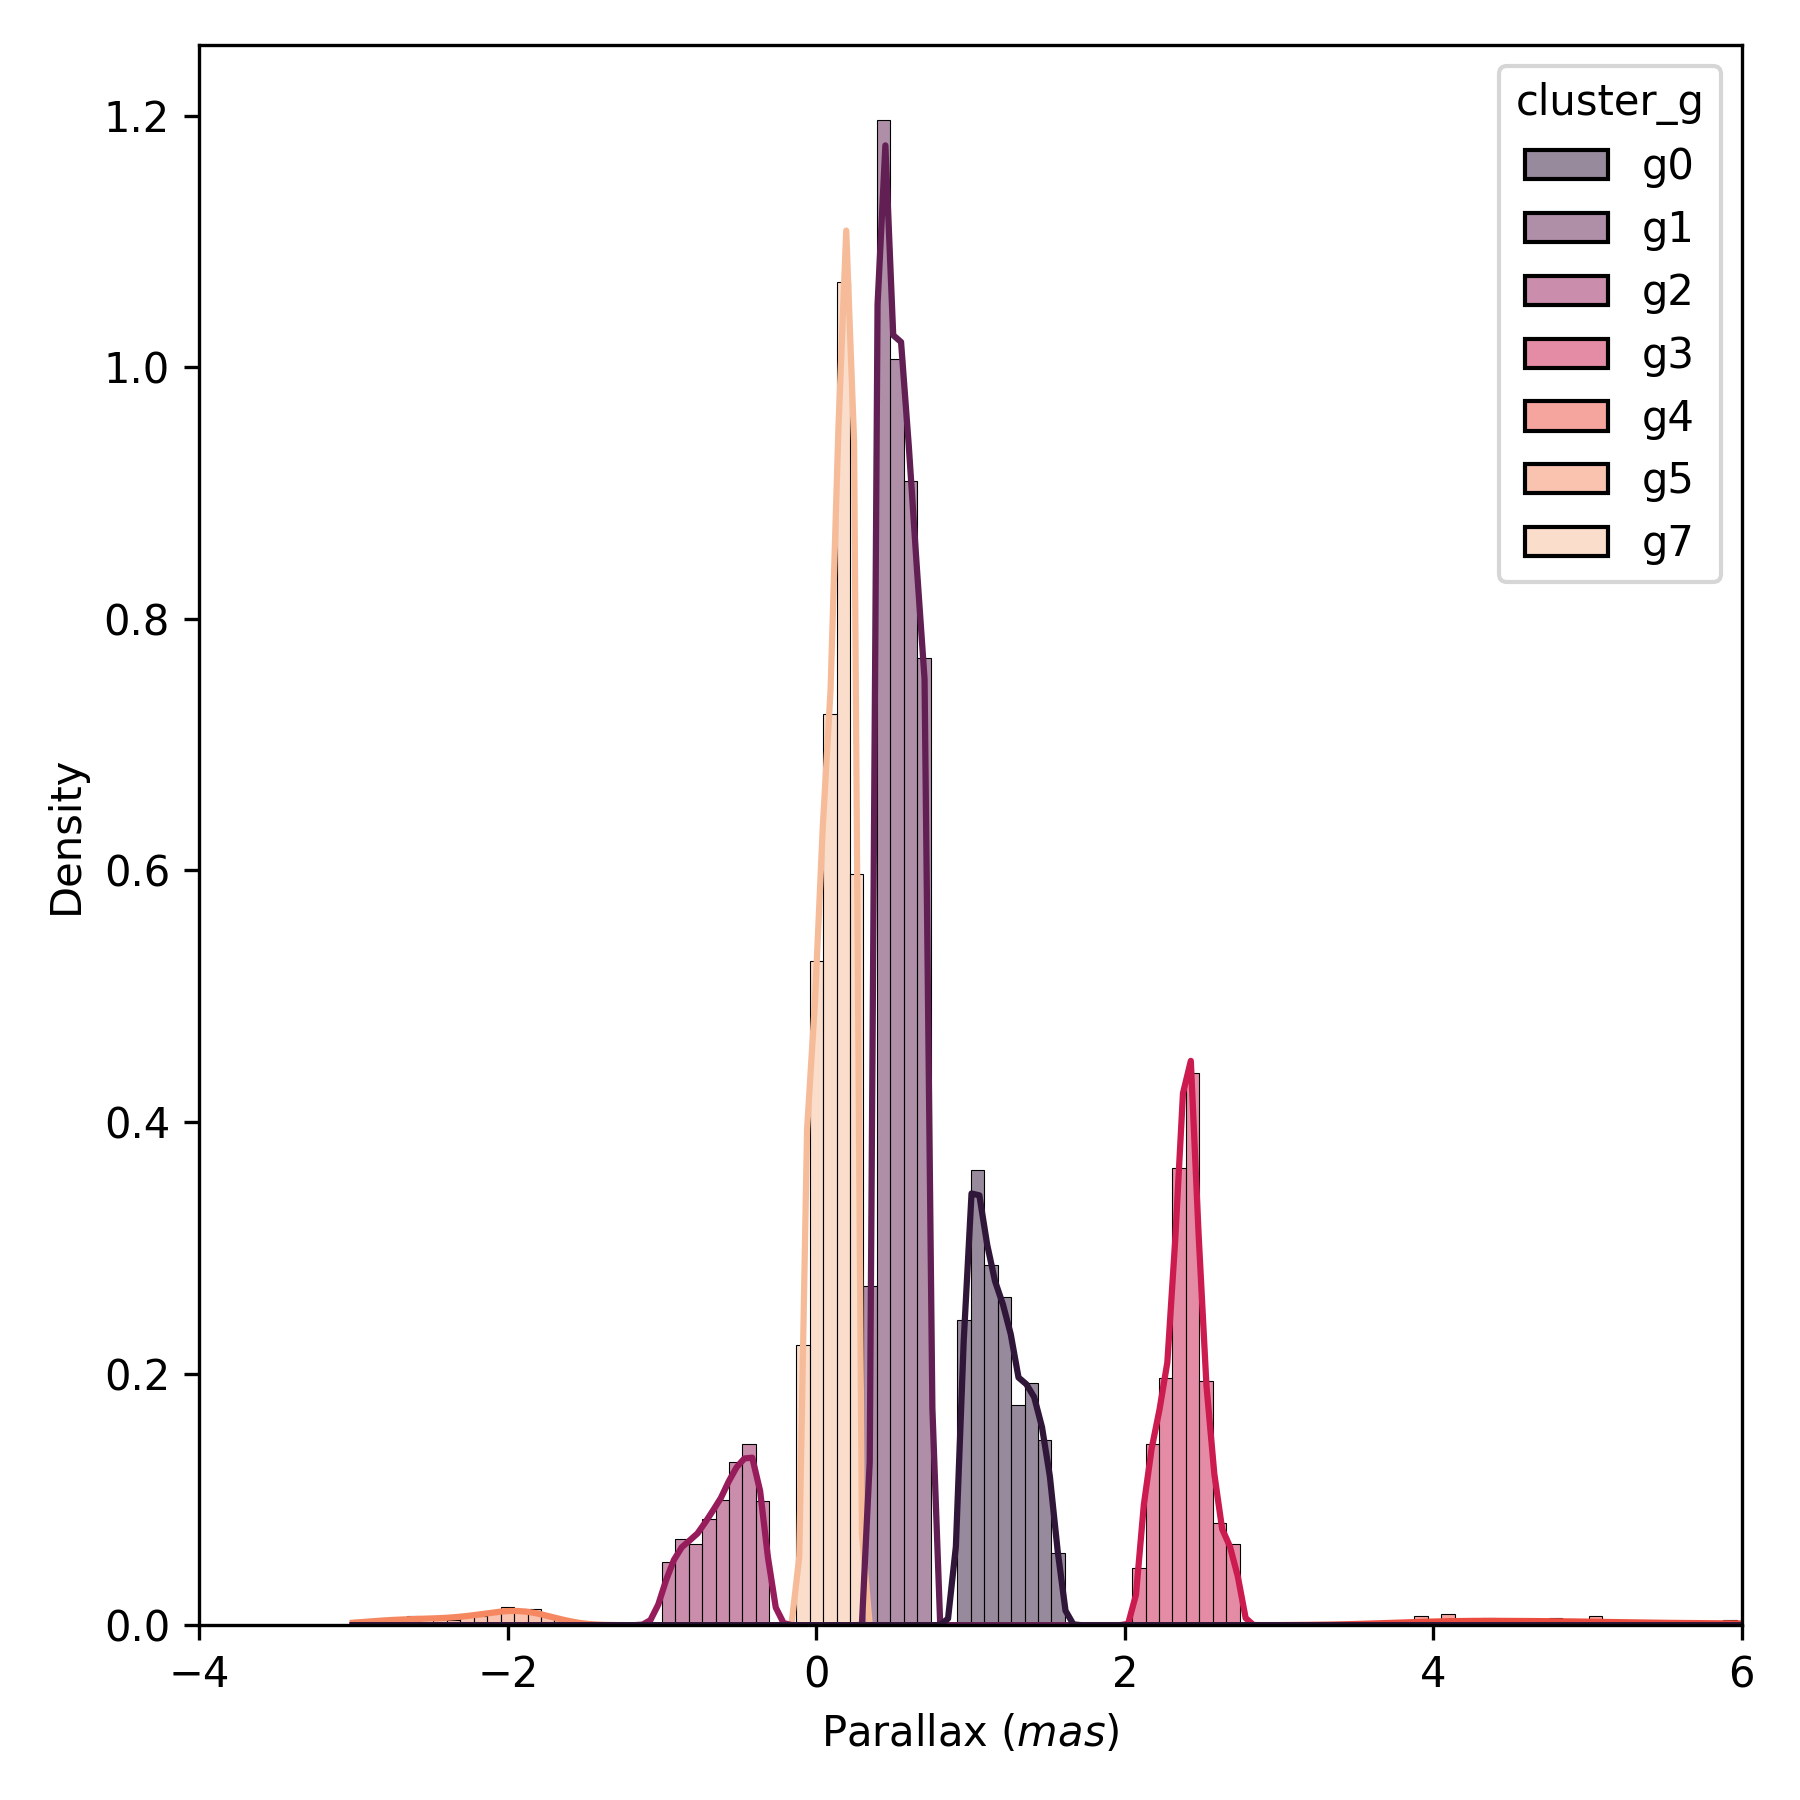
\includegraphics[width=\textwidth]{../figures/ngc_2516/dec_parallax_filtered_ngc_2516.png}
  \end{subfigure}

  \rotatebox[origin=c]{90}{{\bfseries } \strut}
  \rotatebox[origin=c]{90}{hr diagram\strut}
  \begin{subfigure}{0.29\textwidth}
    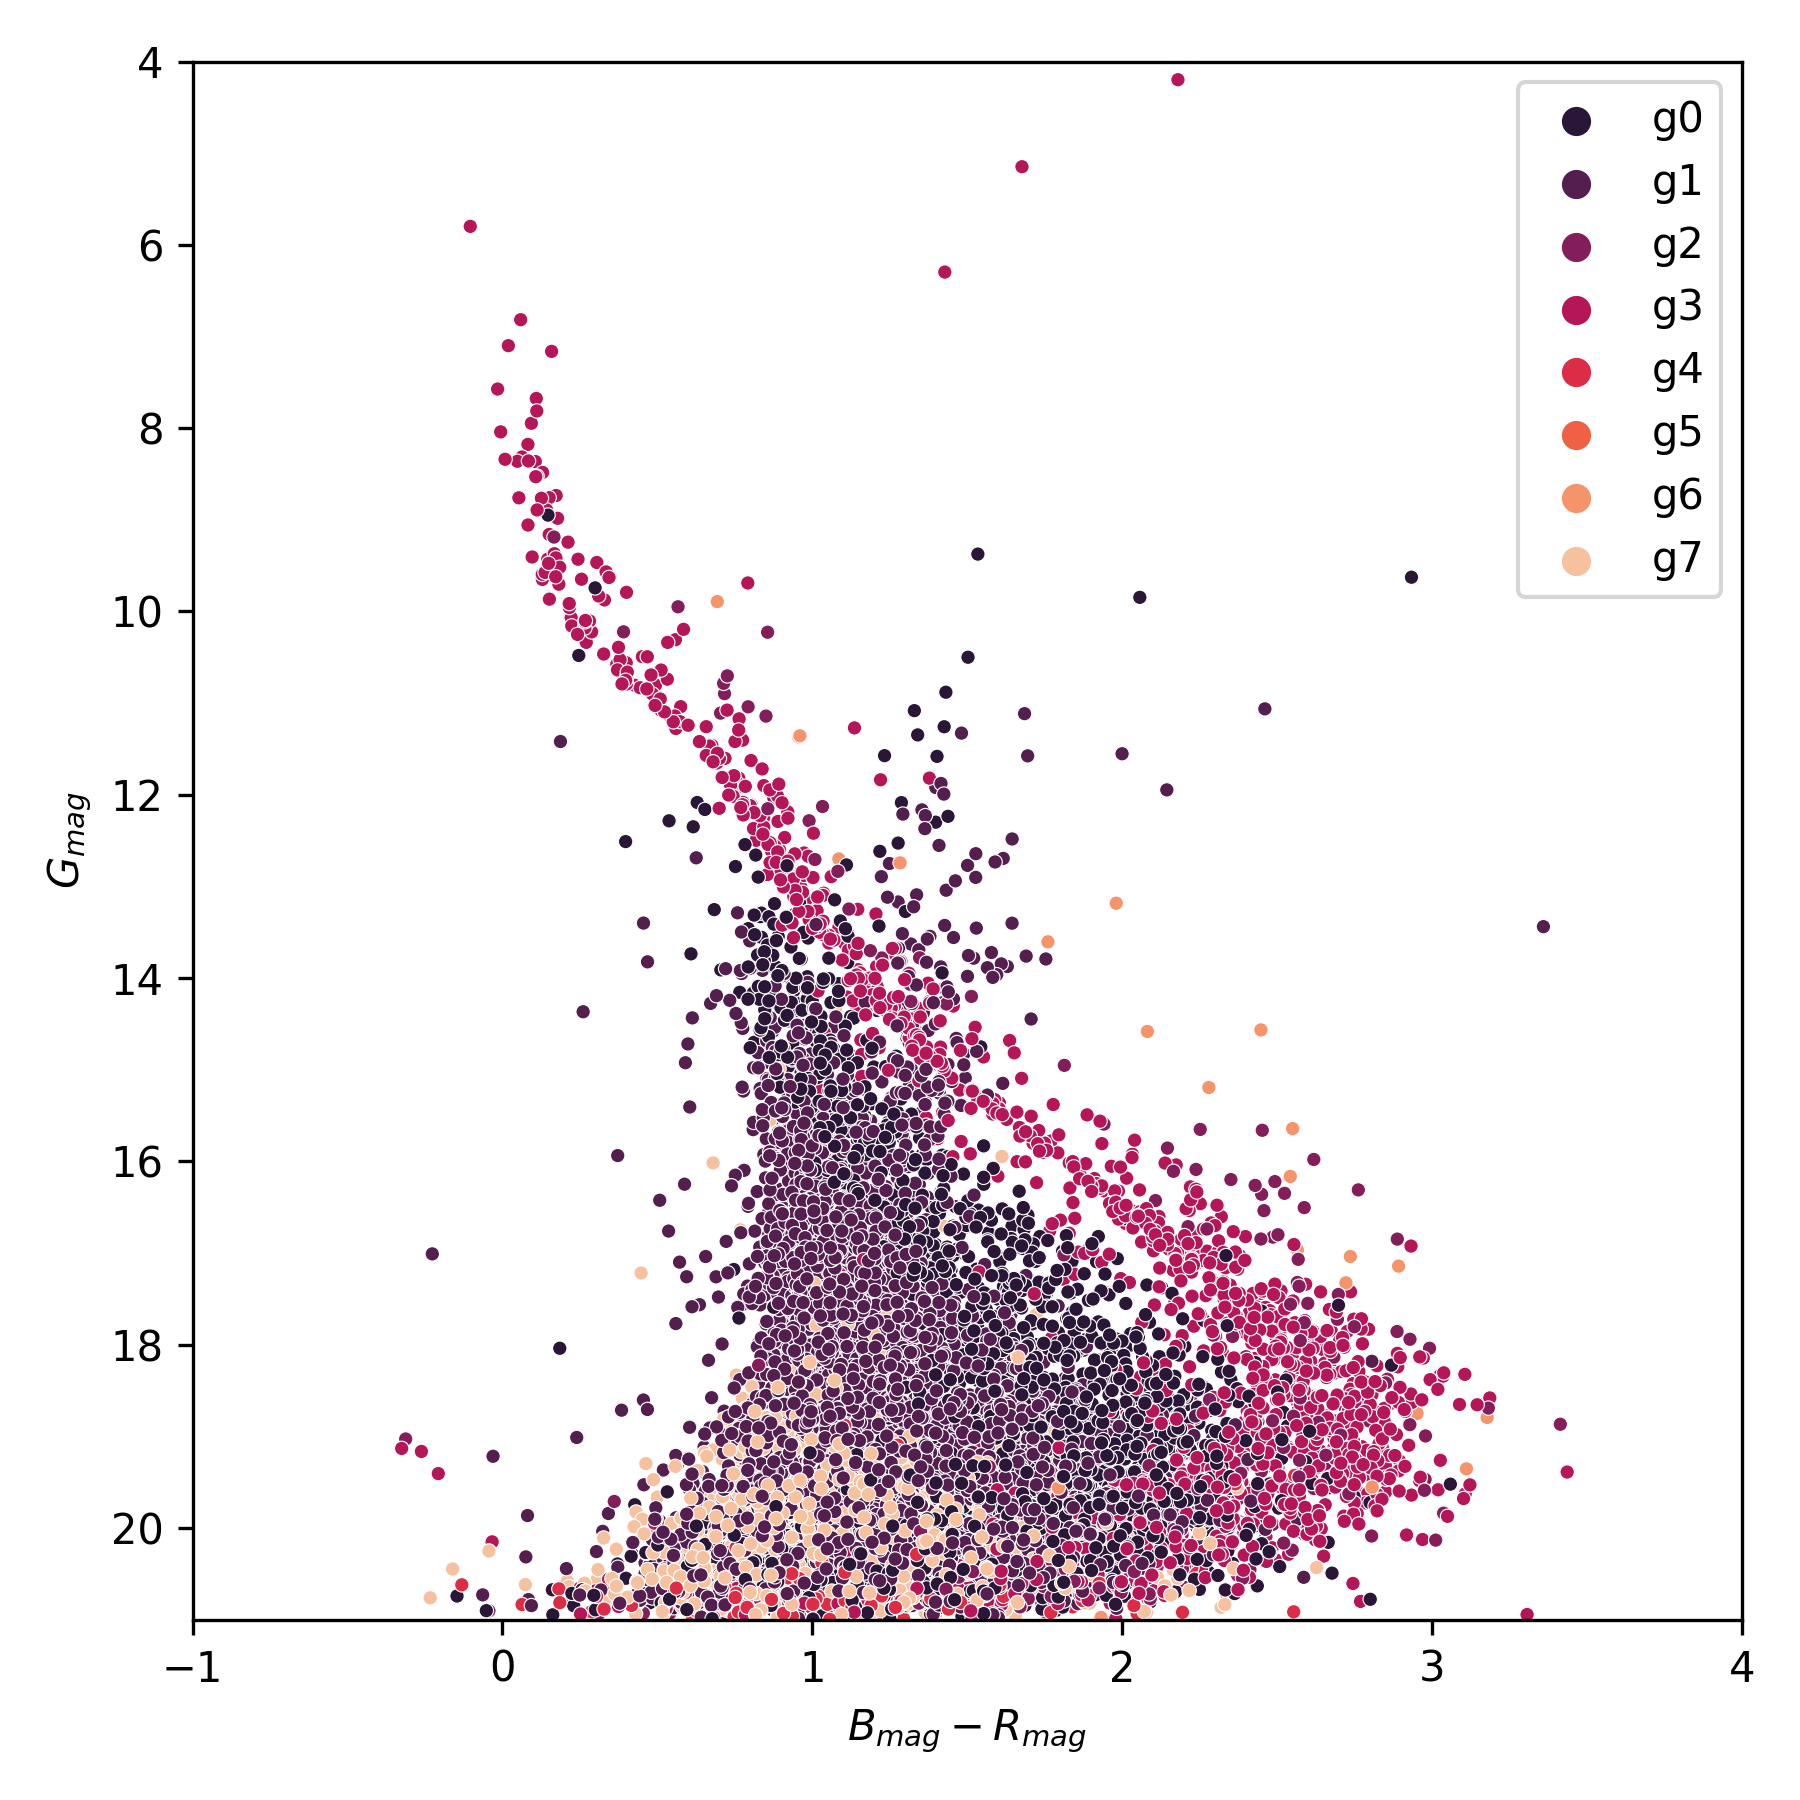
\includegraphics[width=\textwidth]{../figures/ngc_2516/kmeans_hr_diagram_ngc_2516.png}
  \end{subfigure}
  \begin{subfigure}{0.29\textwidth}
    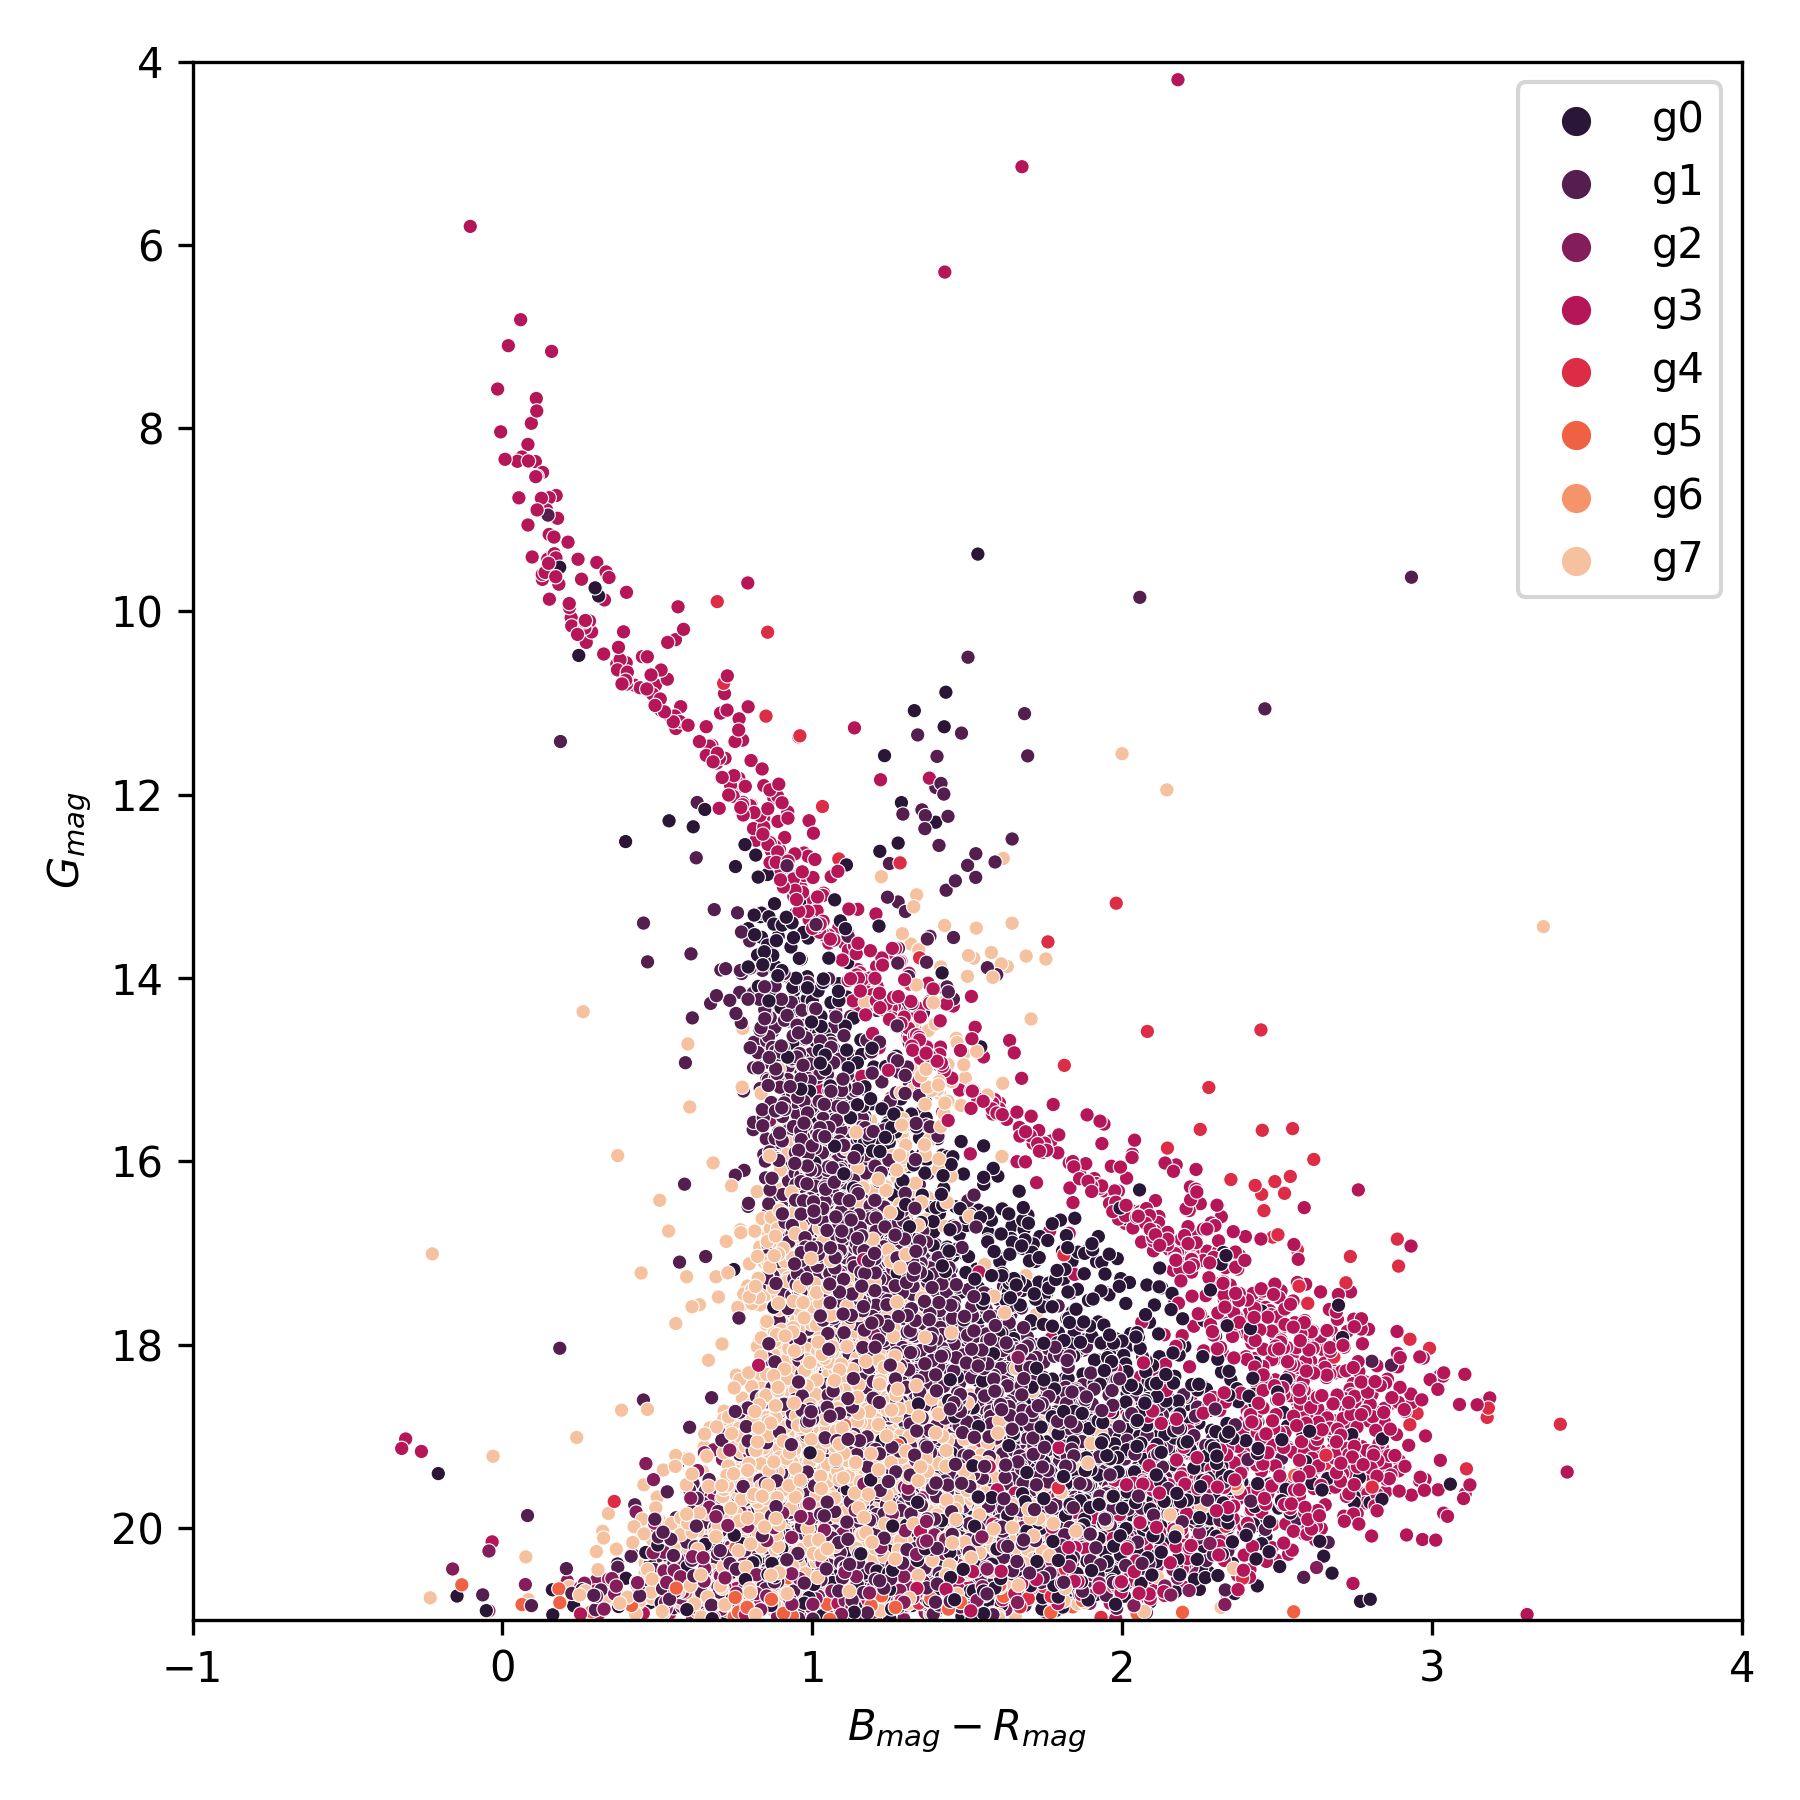
\includegraphics[width=\textwidth]{../figures/ngc_2516/dec_hr_diagram_ngc_2516.png}
  \end{subfigure}
  \begin{subfigure}{0.29\textwidth}
    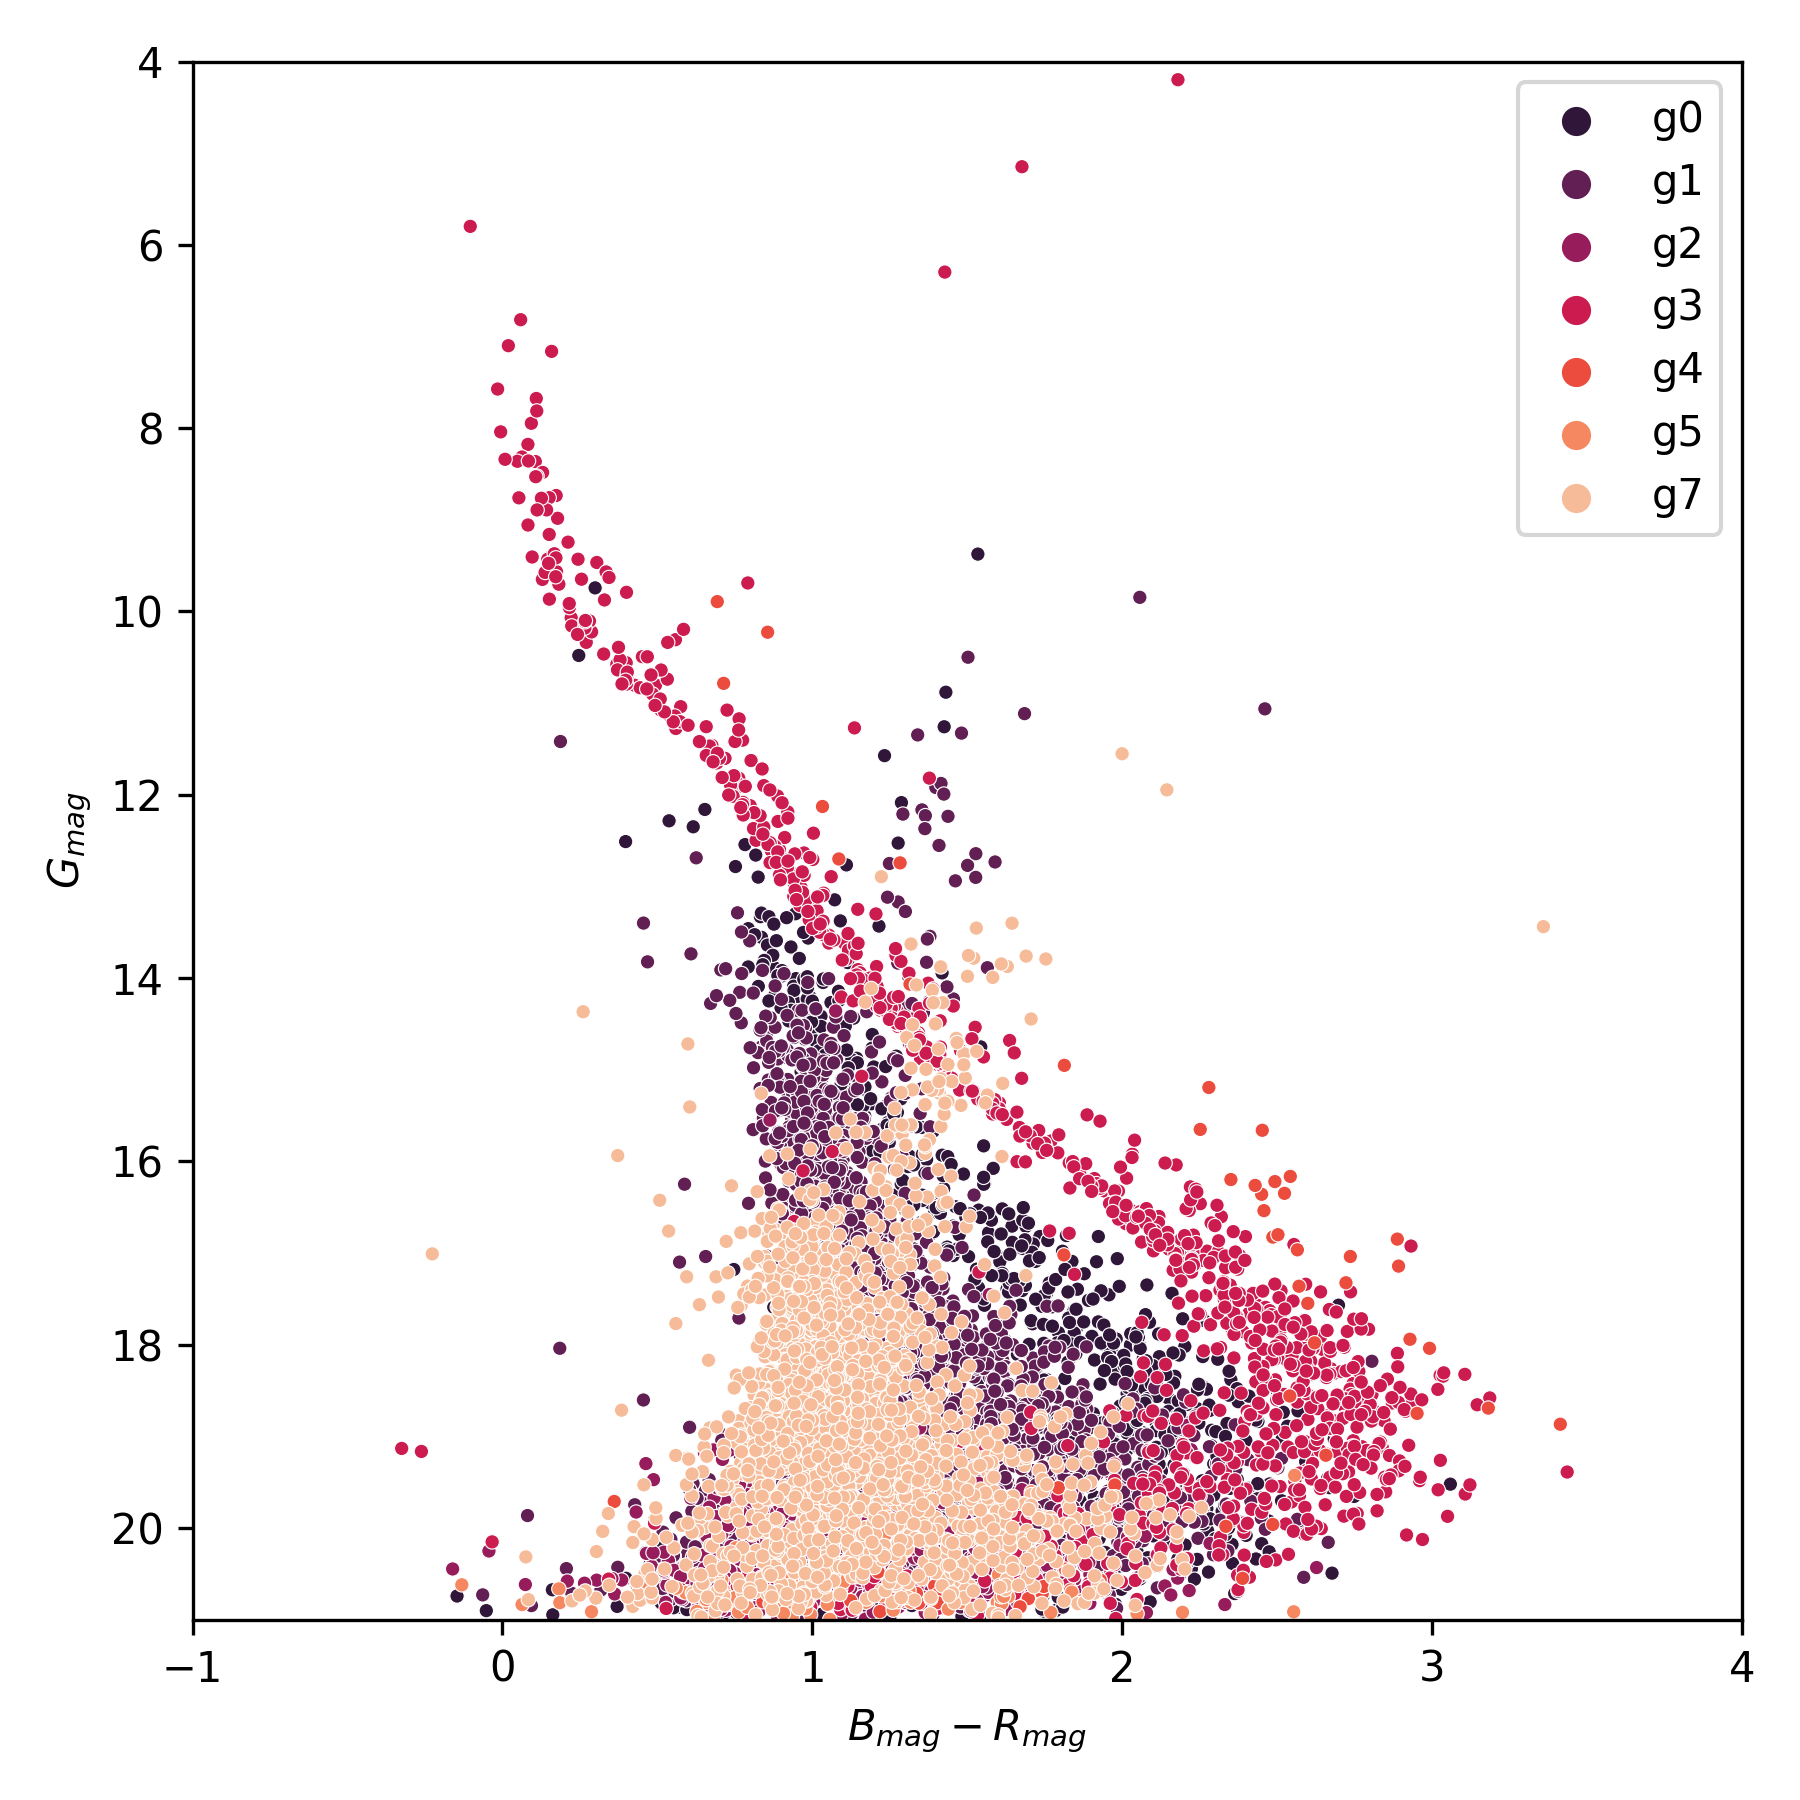
\includegraphics[width=\textwidth]{../figures/ngc_2516/dec_hr_diagram_filtered_ngc_2516.png}
  \end{subfigure}

  \rotatebox[origin=c]{90}{{\bfseries NGC 2632}\strut}
  \rotatebox[origin=c]{90}{parallax \strut}
  \begin{subfigure}{0.29\textwidth}
    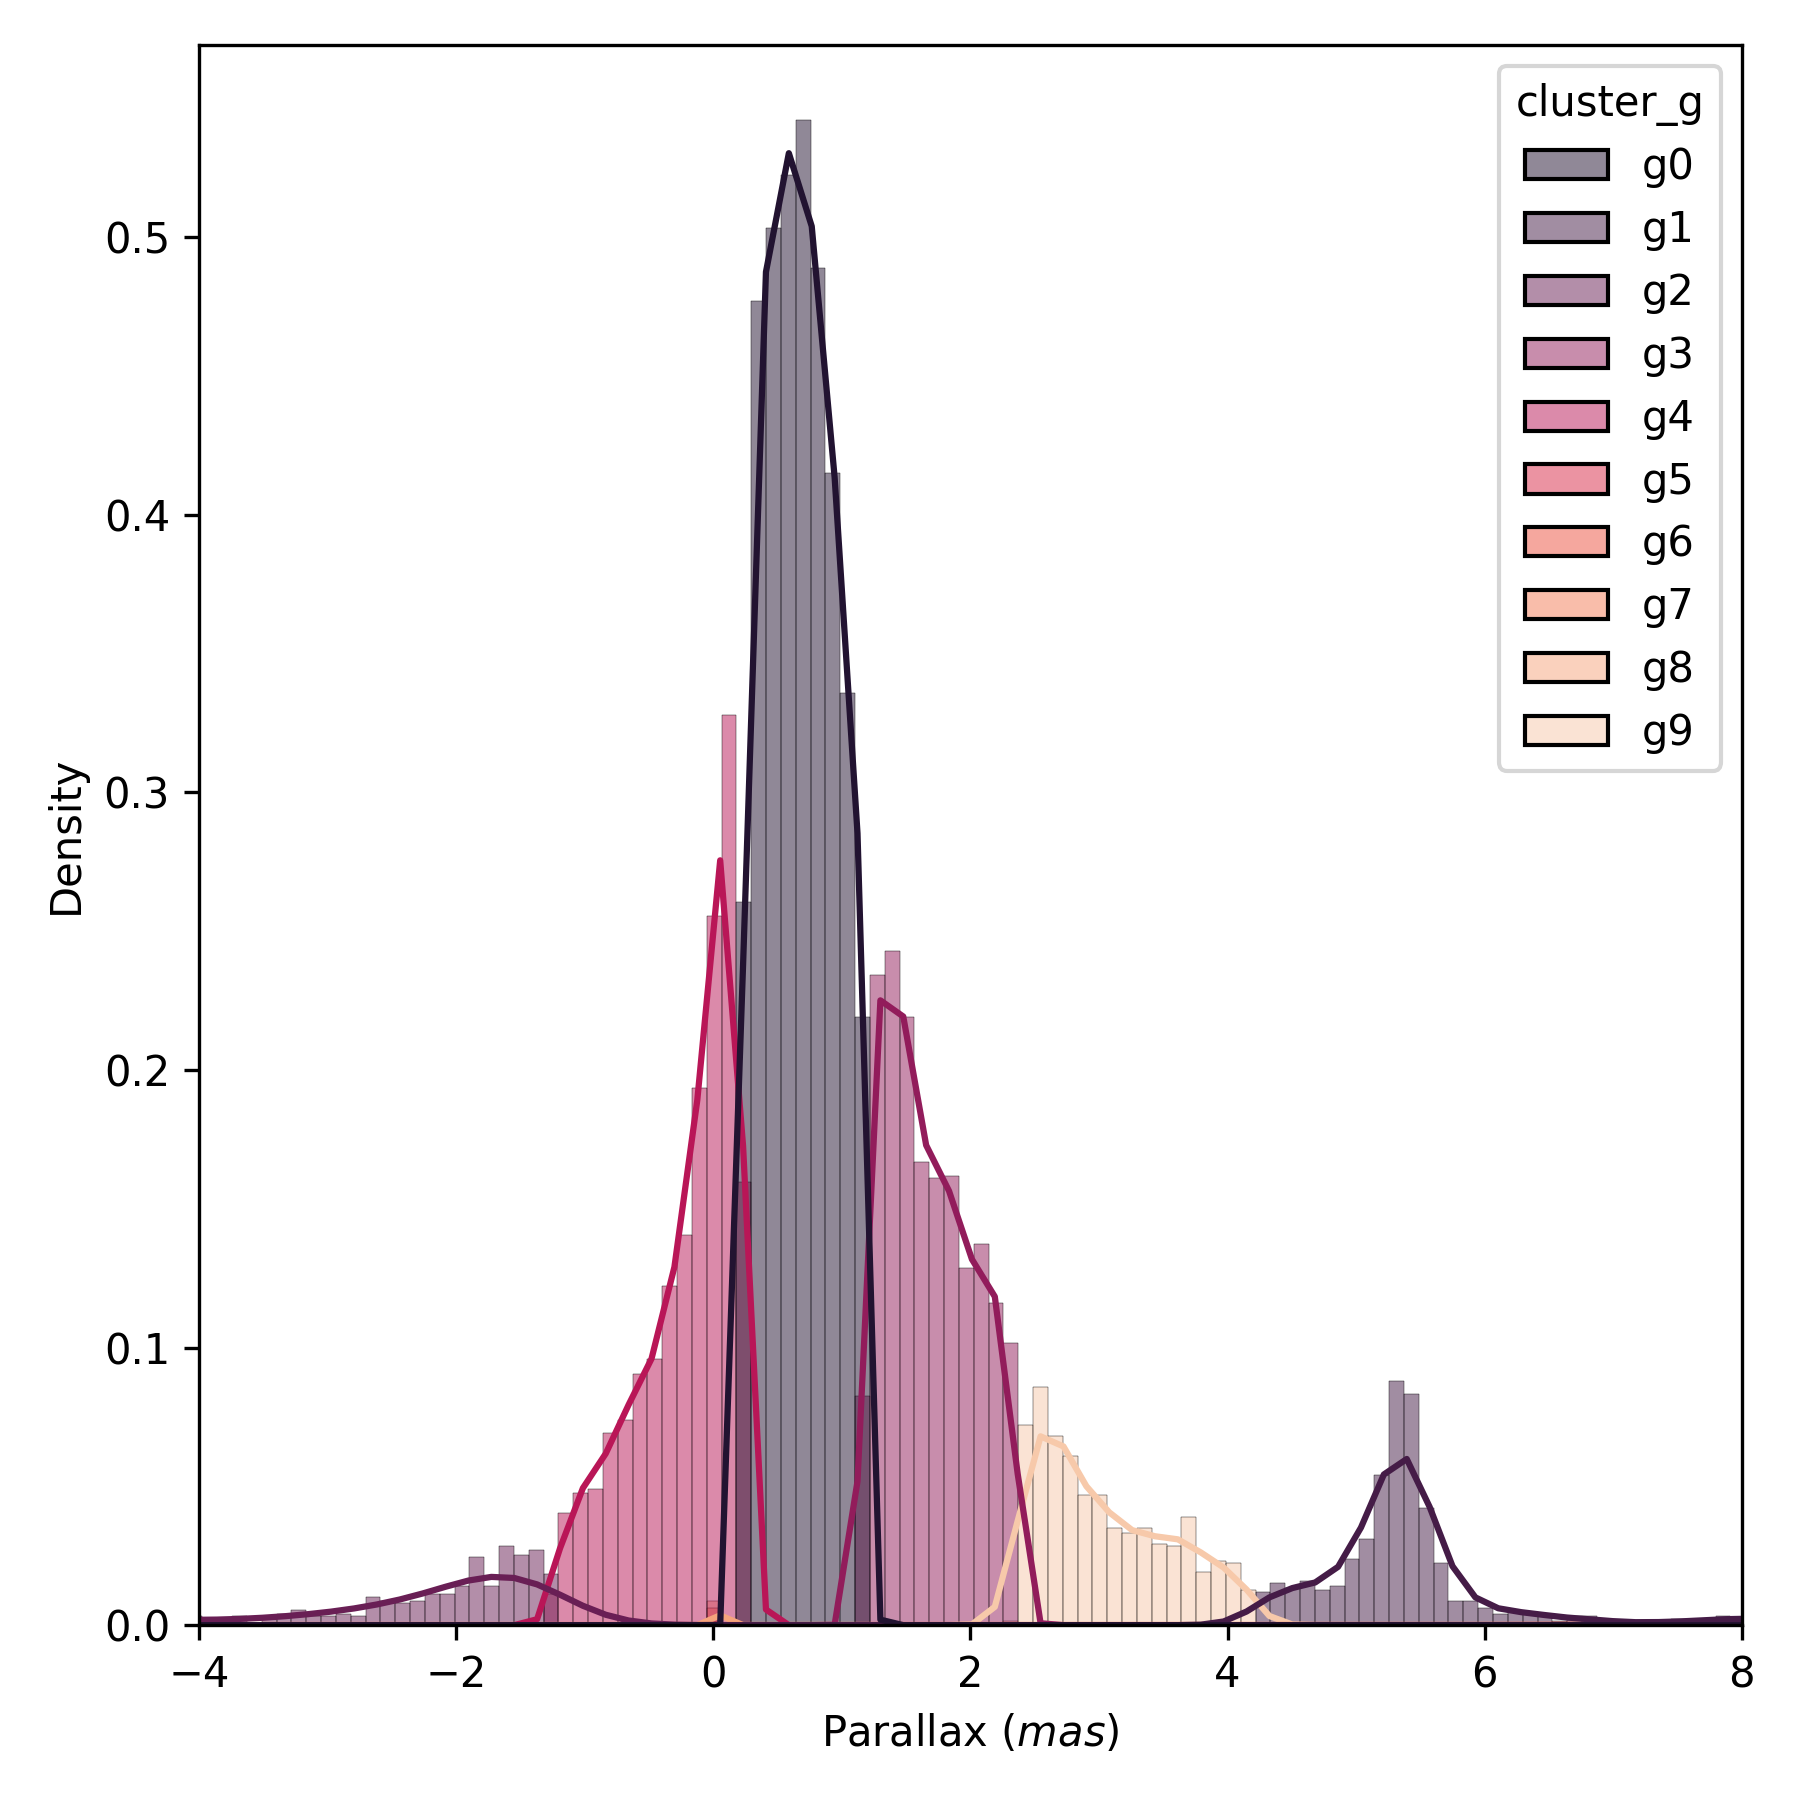
\includegraphics[width=\textwidth]{../figures/ngc_2632/kmeans_parallax_ngc_2632.png}
  \end{subfigure}
  \begin{subfigure}{0.29\textwidth}
    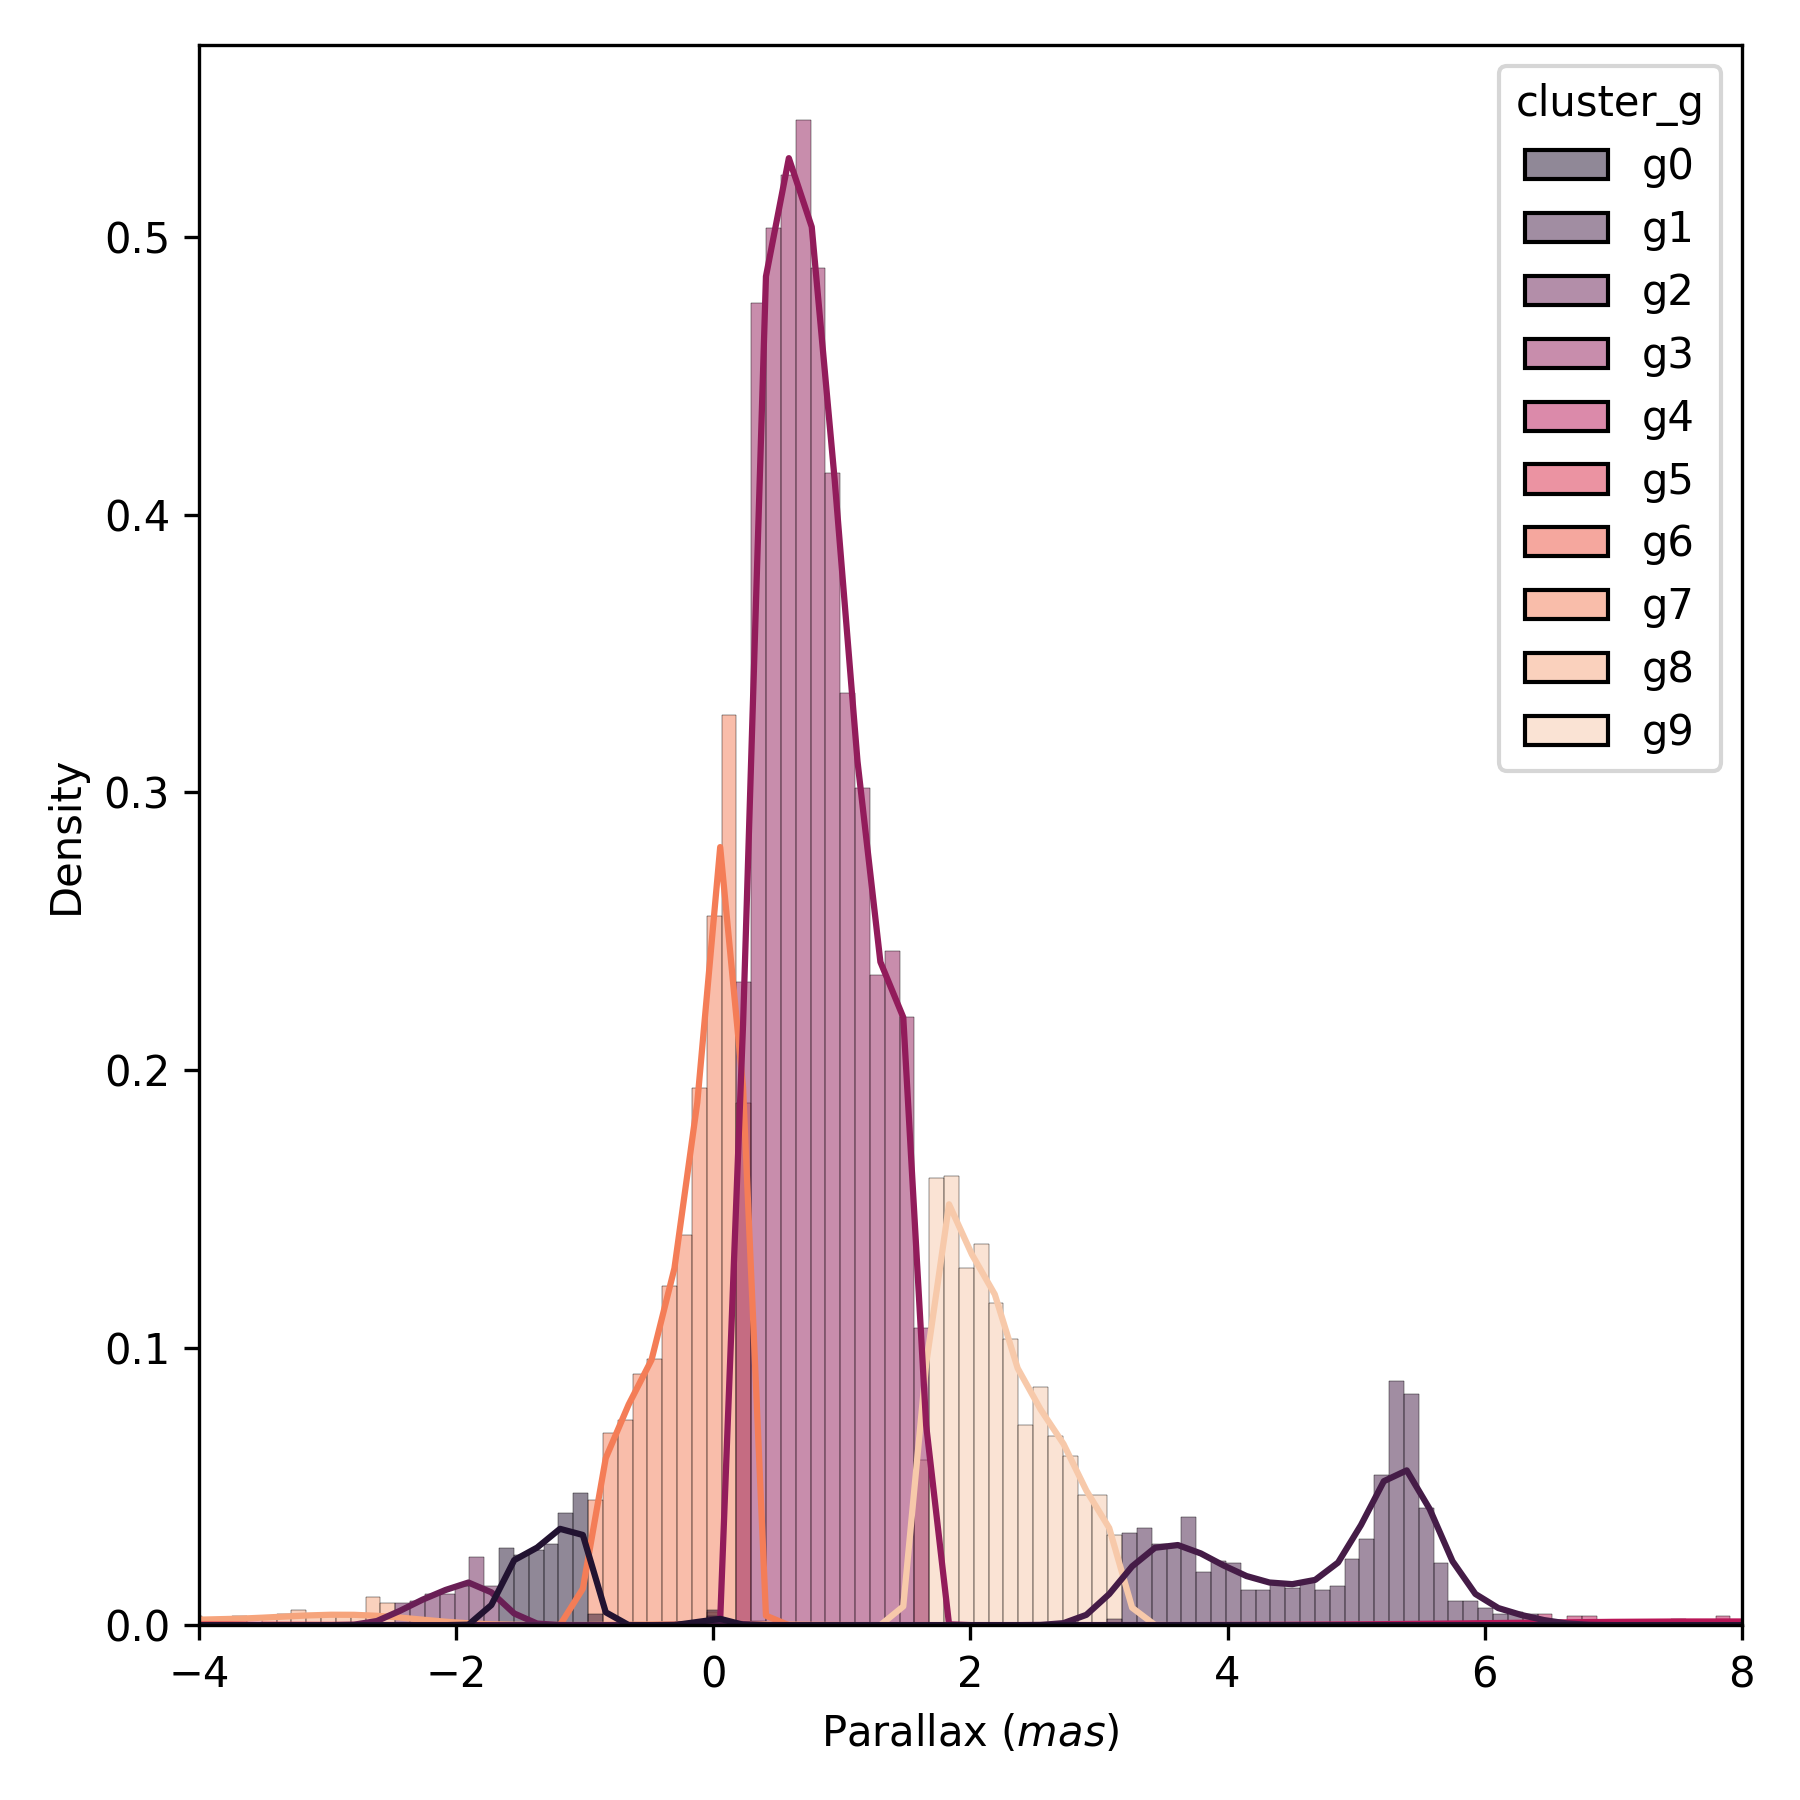
\includegraphics[width=\textwidth]{../figures/ngc_2632/dec_parallax_ngc_2632.png}
  \end{subfigure}
  \begin{subfigure}{0.29\textwidth}
    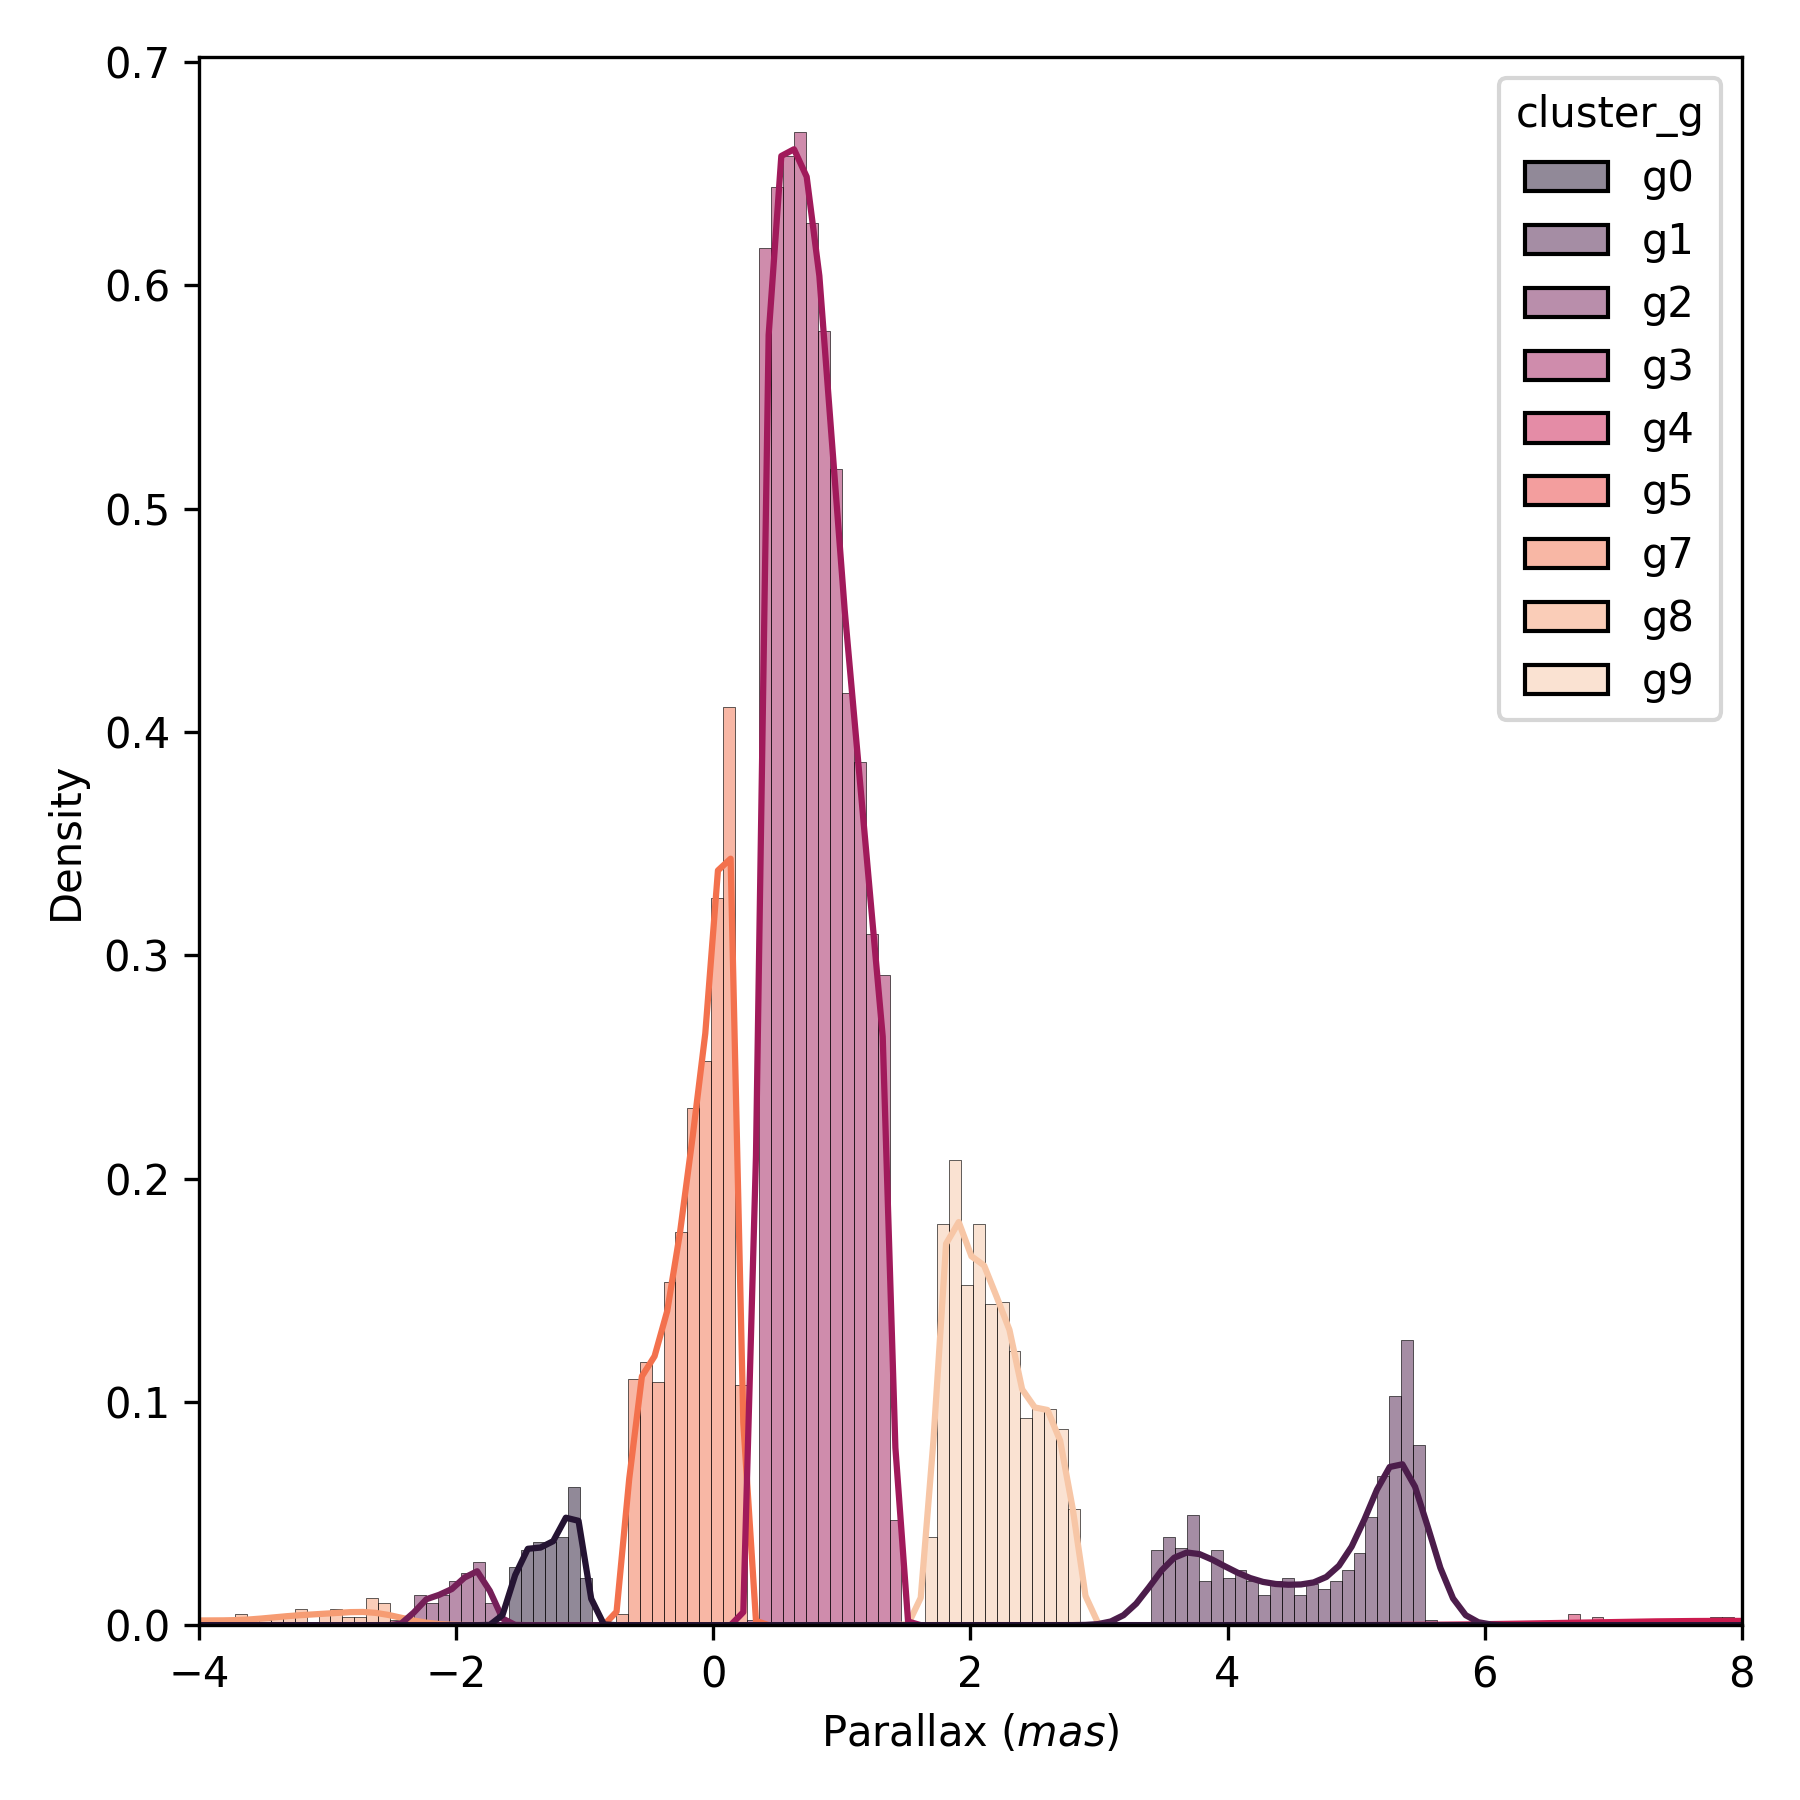
\includegraphics[width=\textwidth]{../figures/ngc_2632/dec_parallax_filtered_ngc_2632.png}
  \end{subfigure}

  \rotatebox[origin=c]{90}{{\bfseries } \strut}
  \rotatebox[origin=c]{90}{hr diagram\strut}
  \begin{subfigure}{0.29\textwidth}
    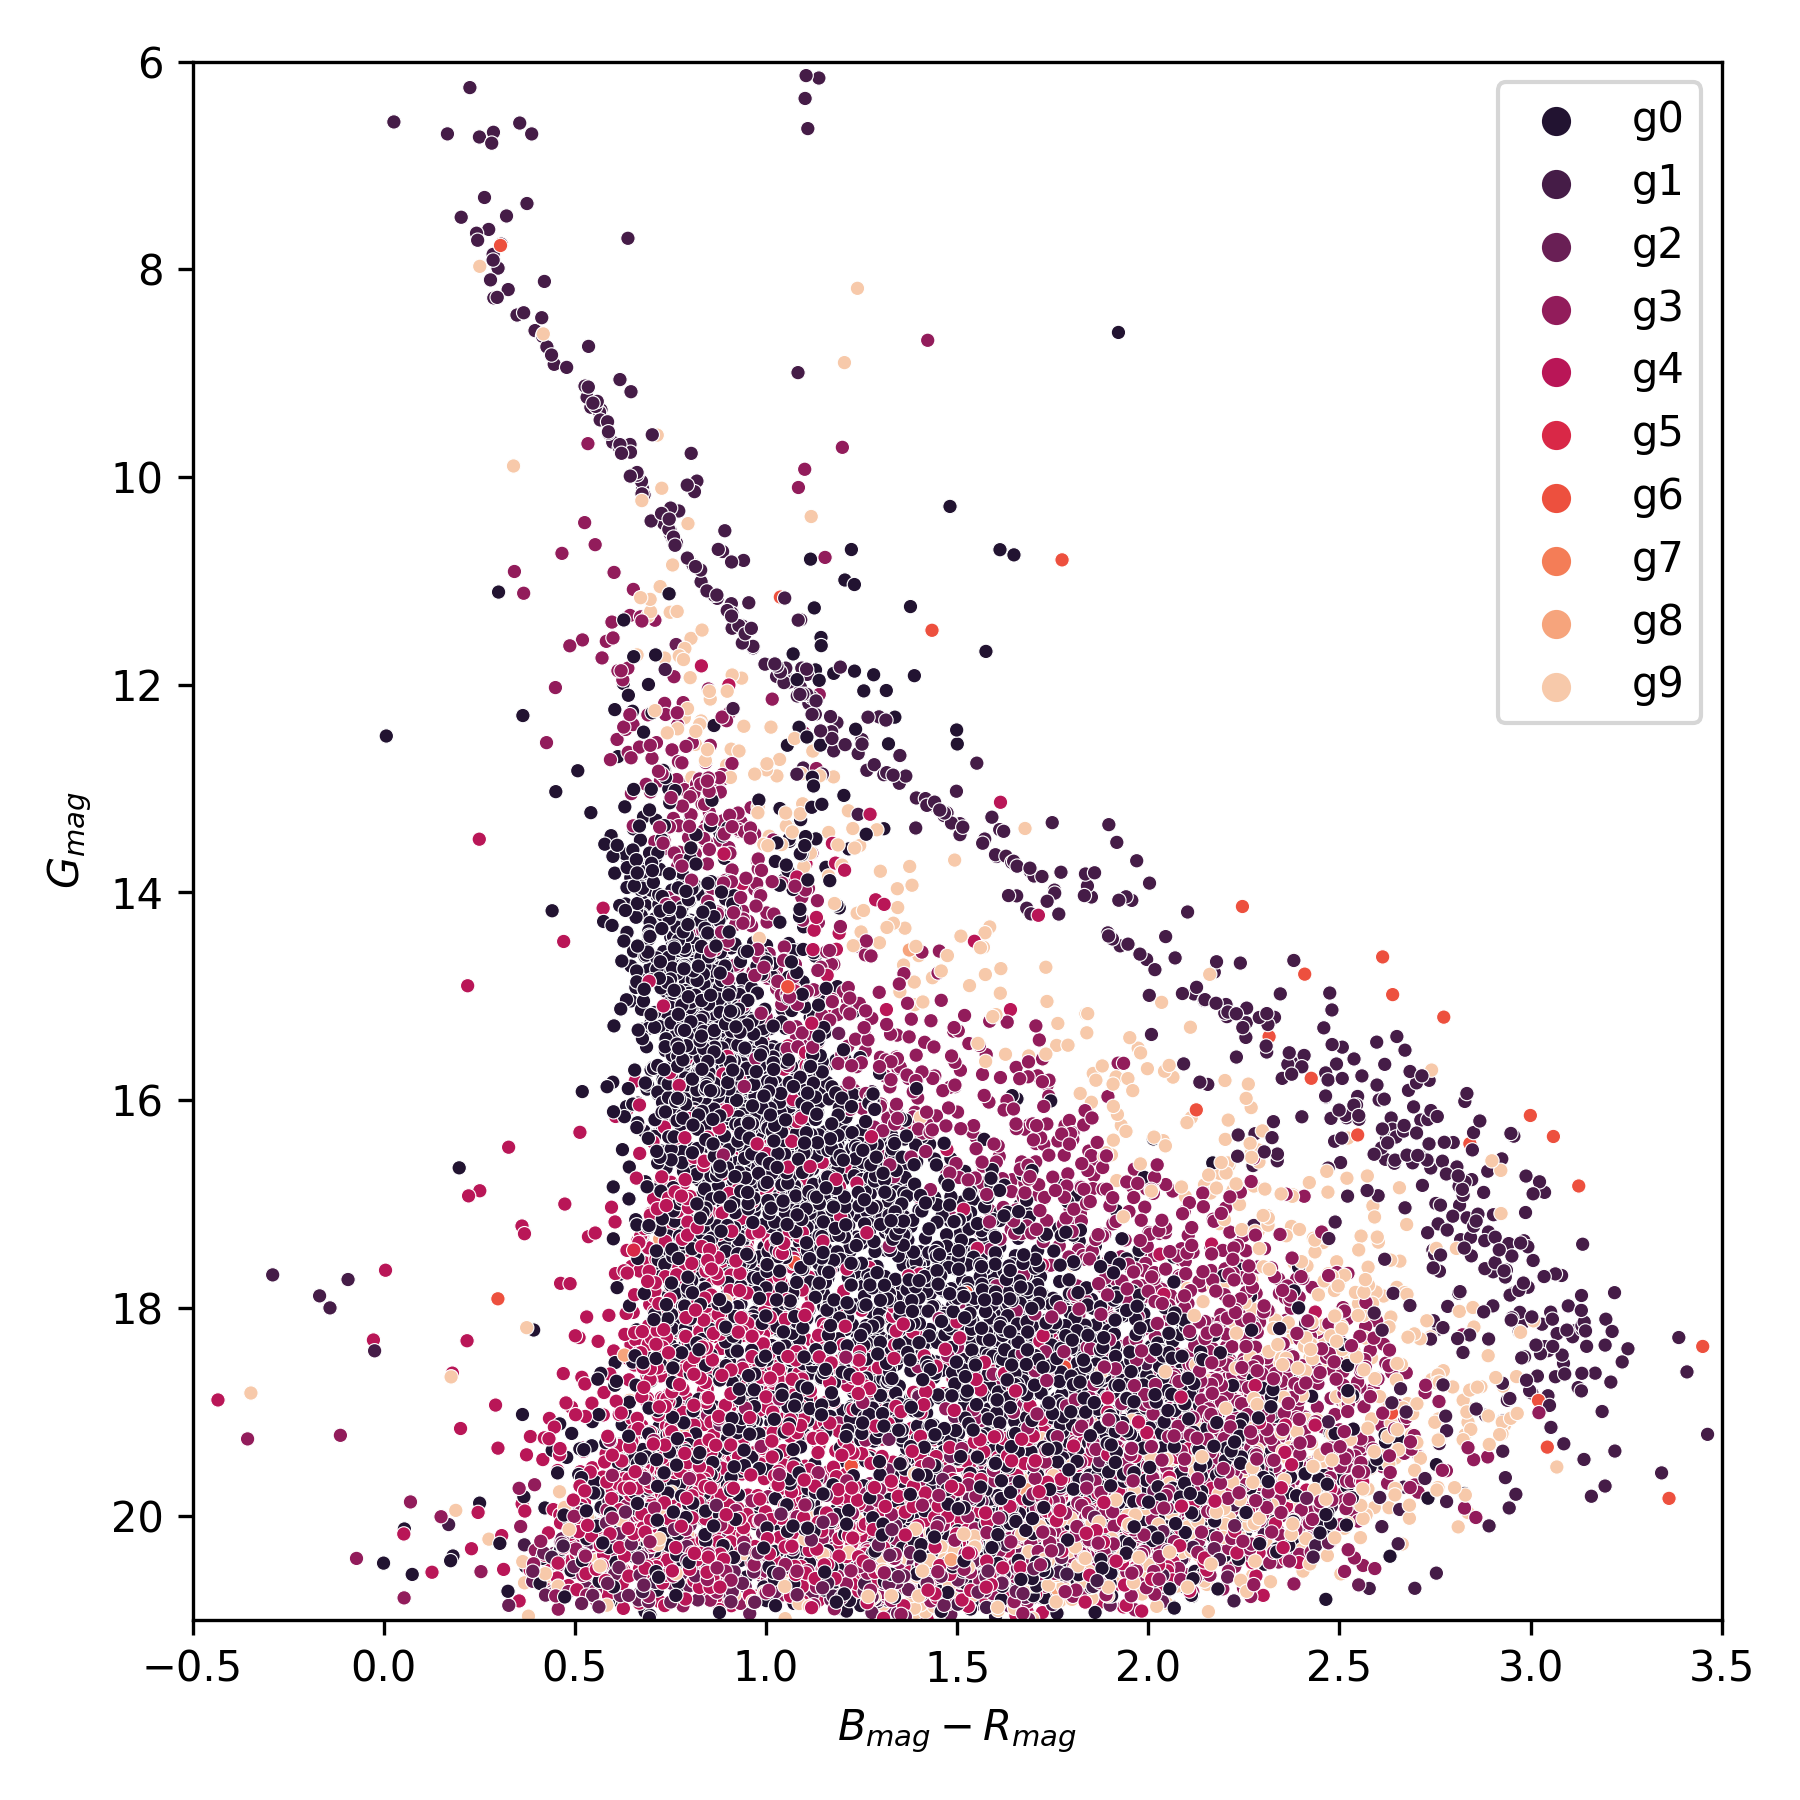
\includegraphics[width=\textwidth]{../figures/ngc_2632/kmeans_hr_diagram_ngc_2632.png}
    \caption{K-Means}
  \end{subfigure}
  \begin{subfigure}{0.29\textwidth}
    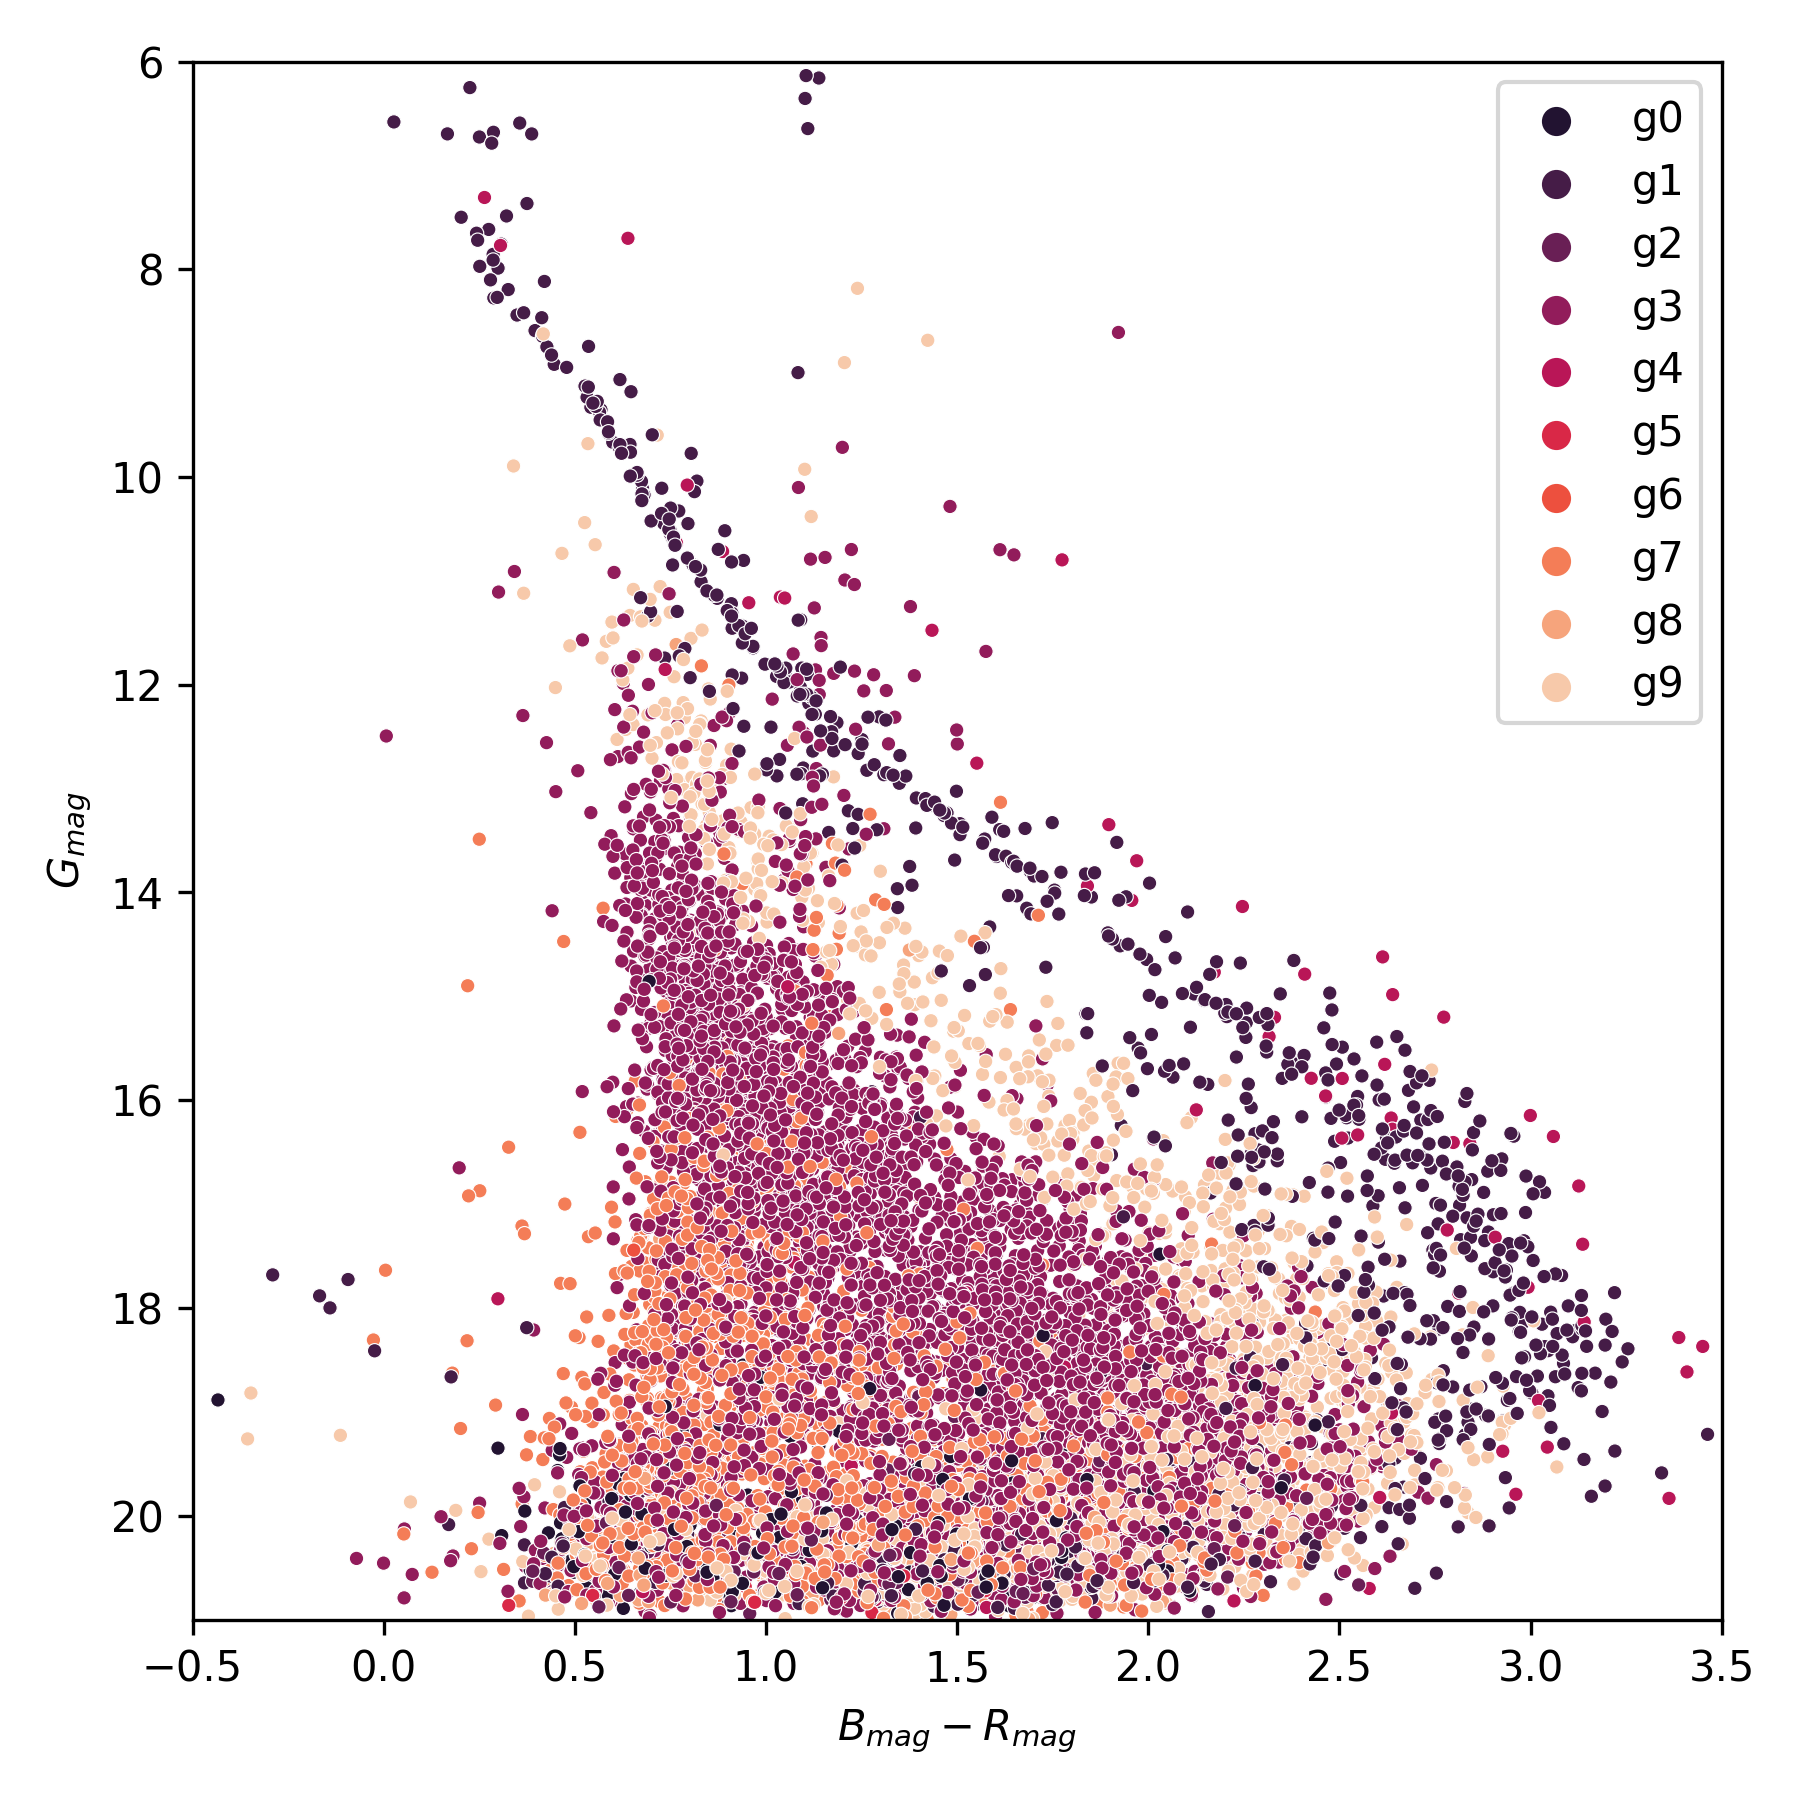
\includegraphics[width=\textwidth]{../figures/ngc_2632/dec_hr_diagram_ngc_2632.png}
    \caption{DECOCC}
  \end{subfigure}%
  \begin{subfigure}{0.29\textwidth}
    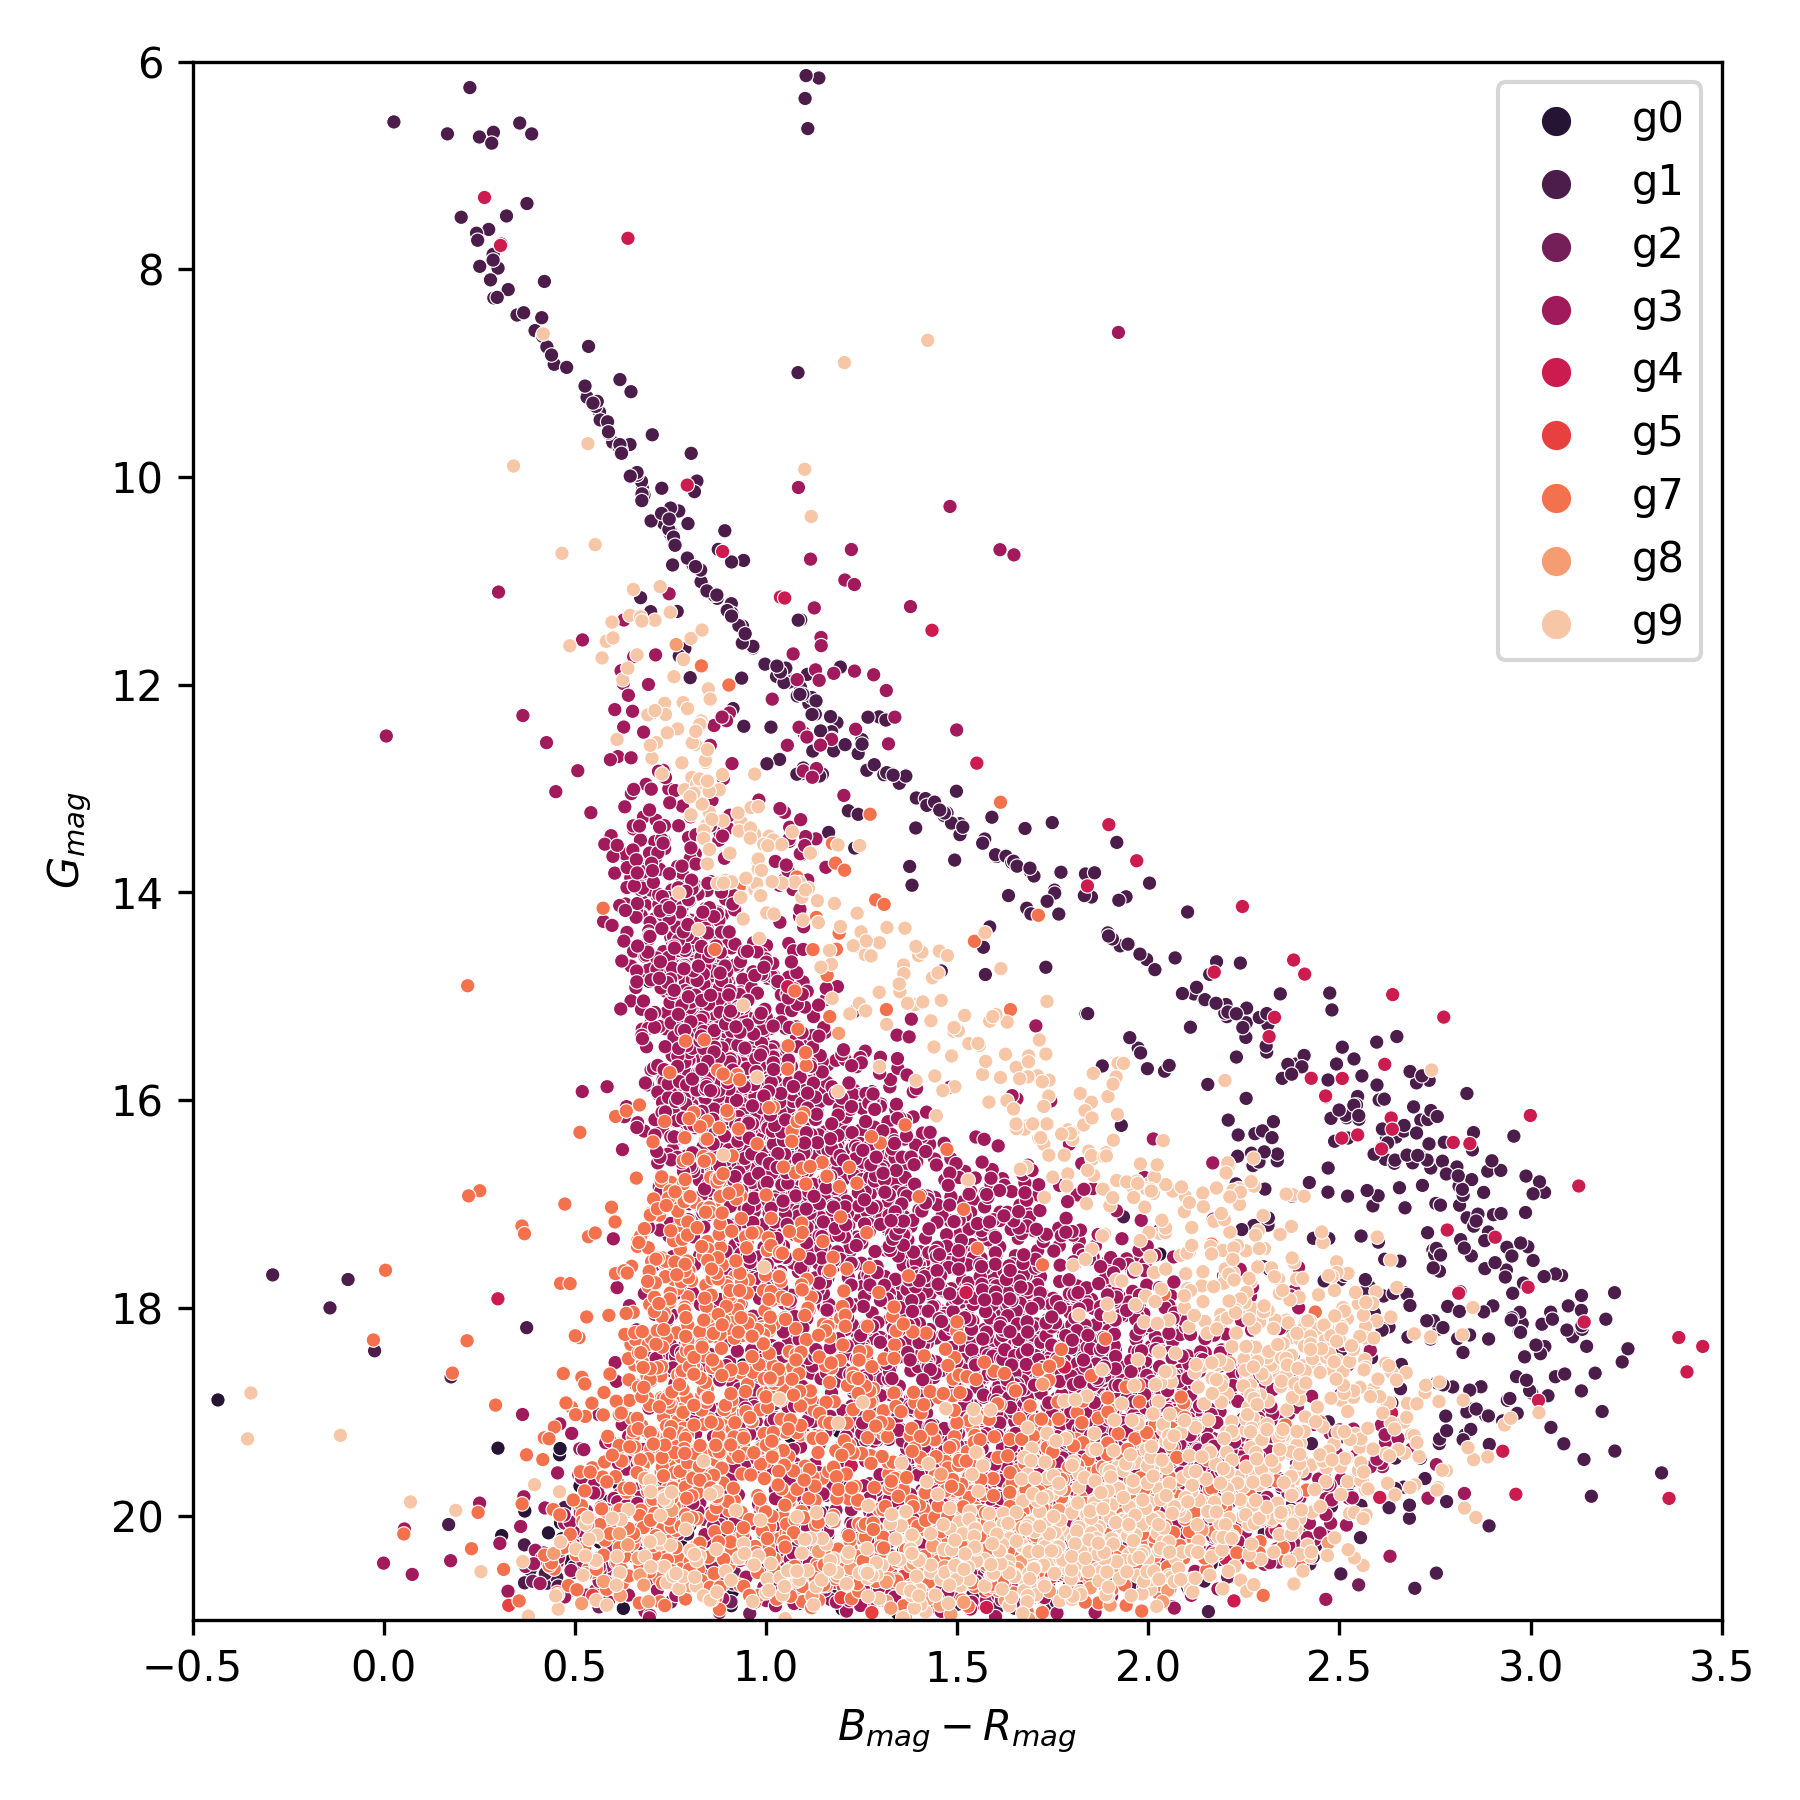
\includegraphics[width=\textwidth]{../figures/ngc_2632/dec_hr_diagram_filtered_ngc_2632.png}
    \caption{DECOCC (filt.)}
  \end{subfigure}
  \caption{Summary of the characterization for the clusters NGC 2516 and NGC 2632.}
  \label{fig:ngc_2516_ngc_2632_characterization_evolution}
\end{figure*}

\begin{figure*}[!hbt]
  \rotatebox[origin=c]{90}{{\bfseries NGC 2682}\strut}
  \rotatebox[origin=c]{90}{parallax \strut}
  \begin{subfigure}{0.29\textwidth}
    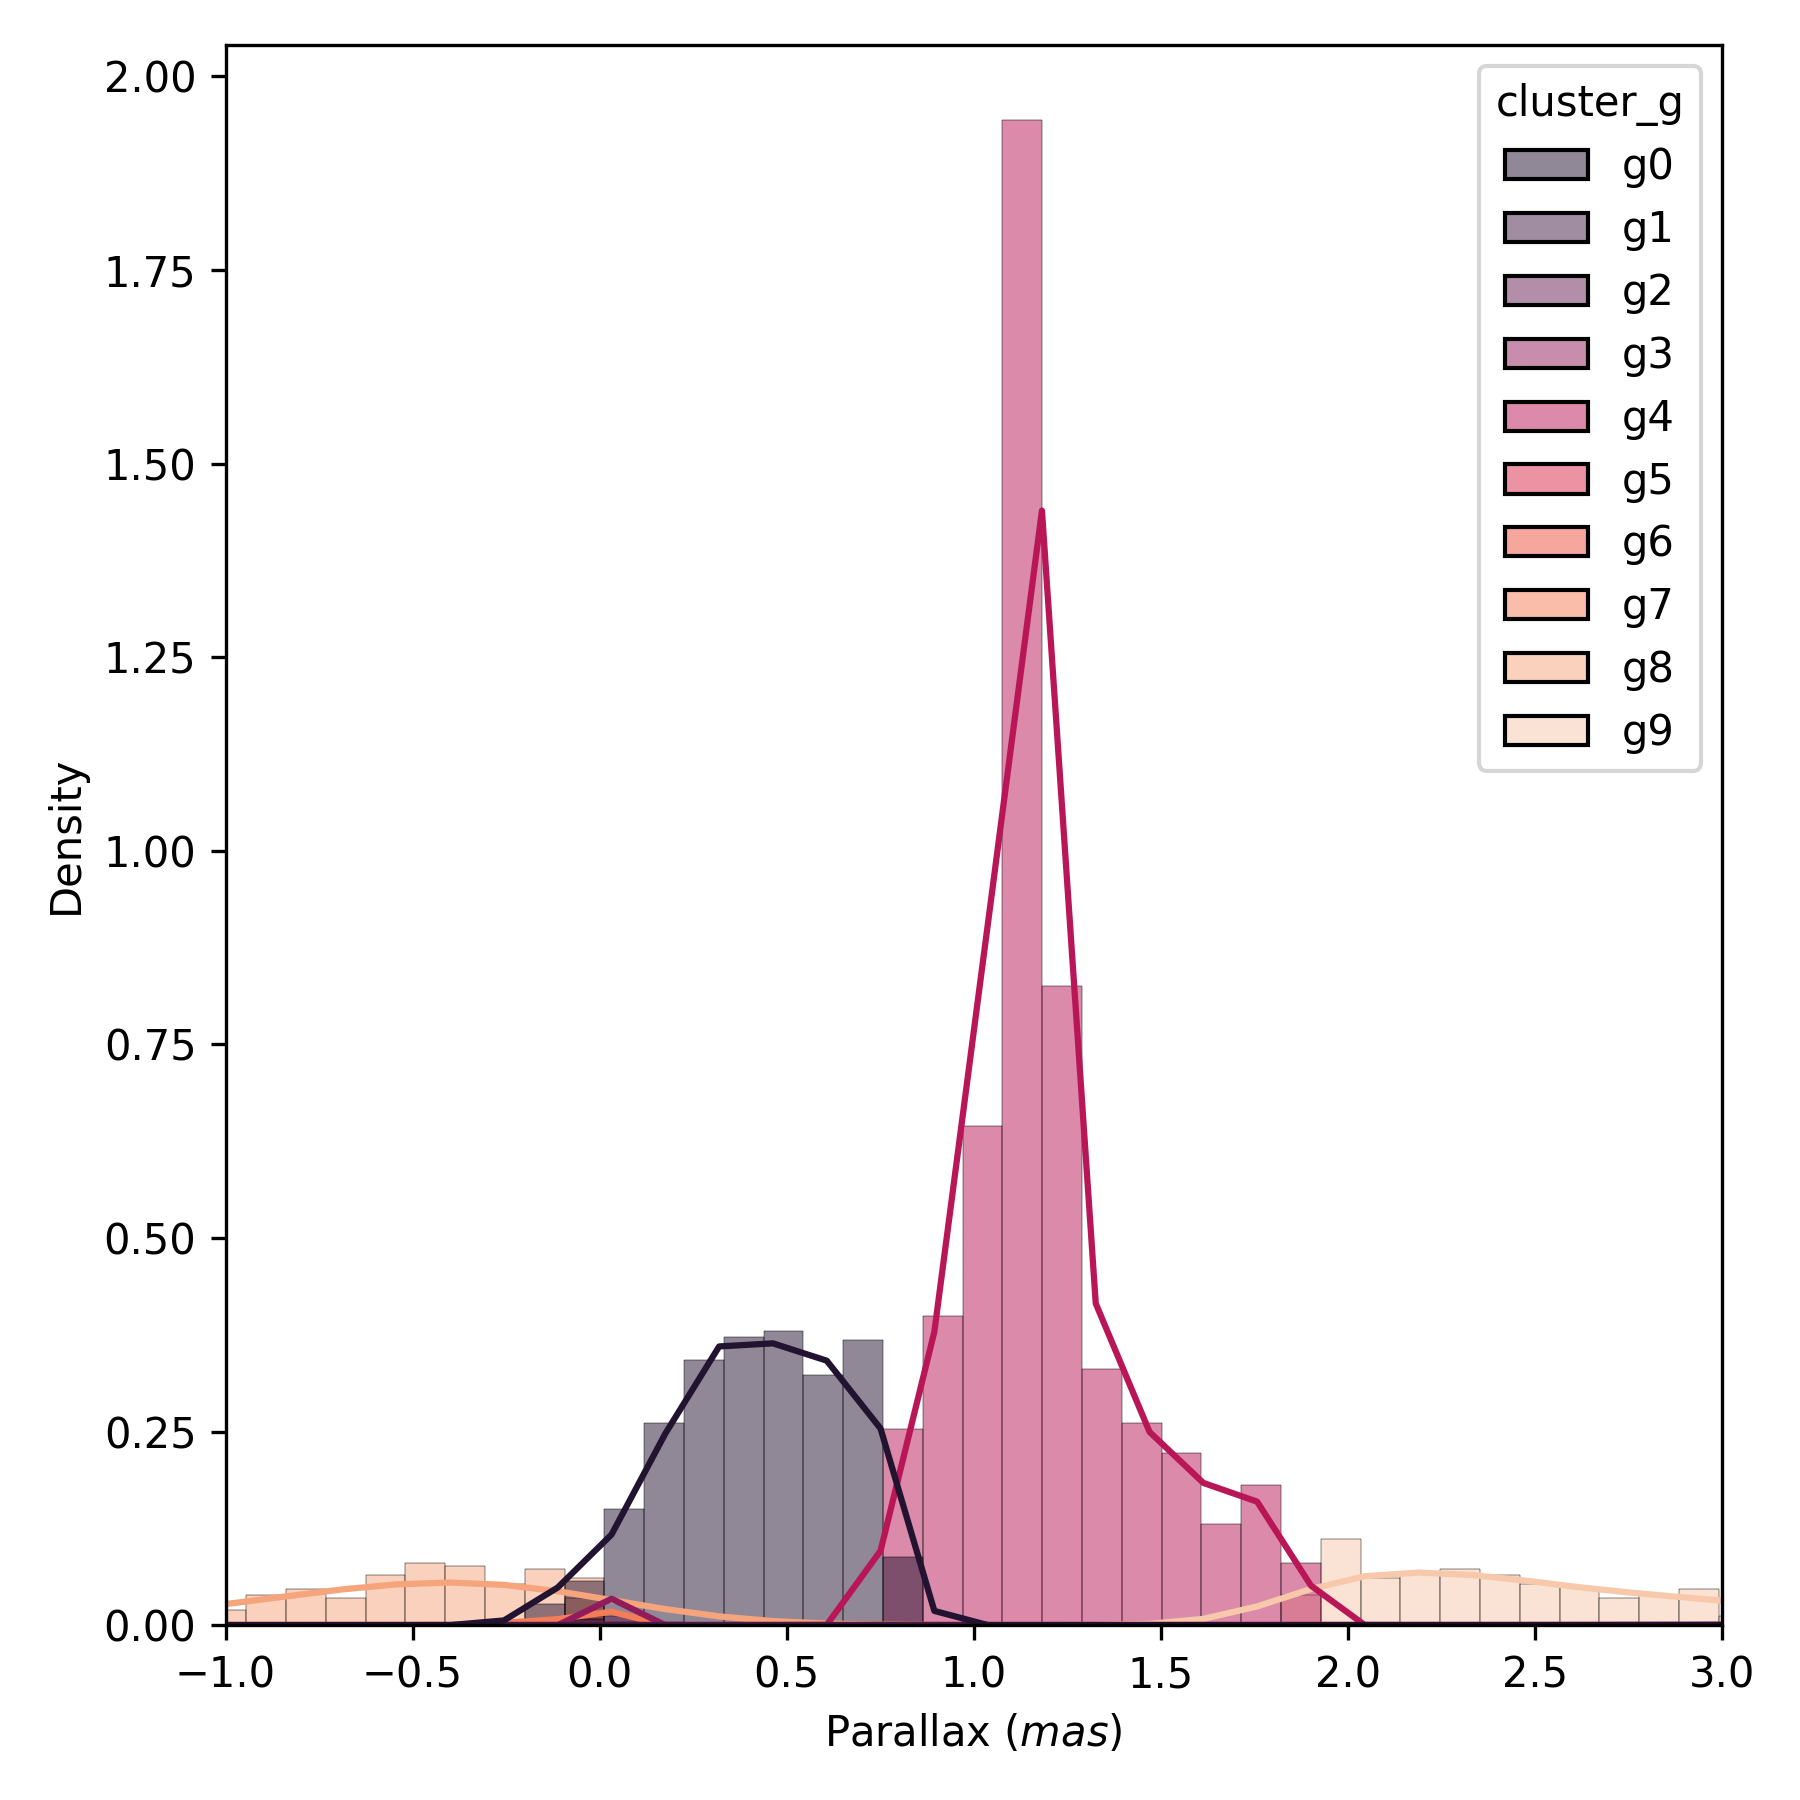
\includegraphics[width=\textwidth]{../figures/ngc_2682/kmeans_parallax_ngc_2682.png}
  \end{subfigure}
  \begin{subfigure}{0.29\textwidth}
    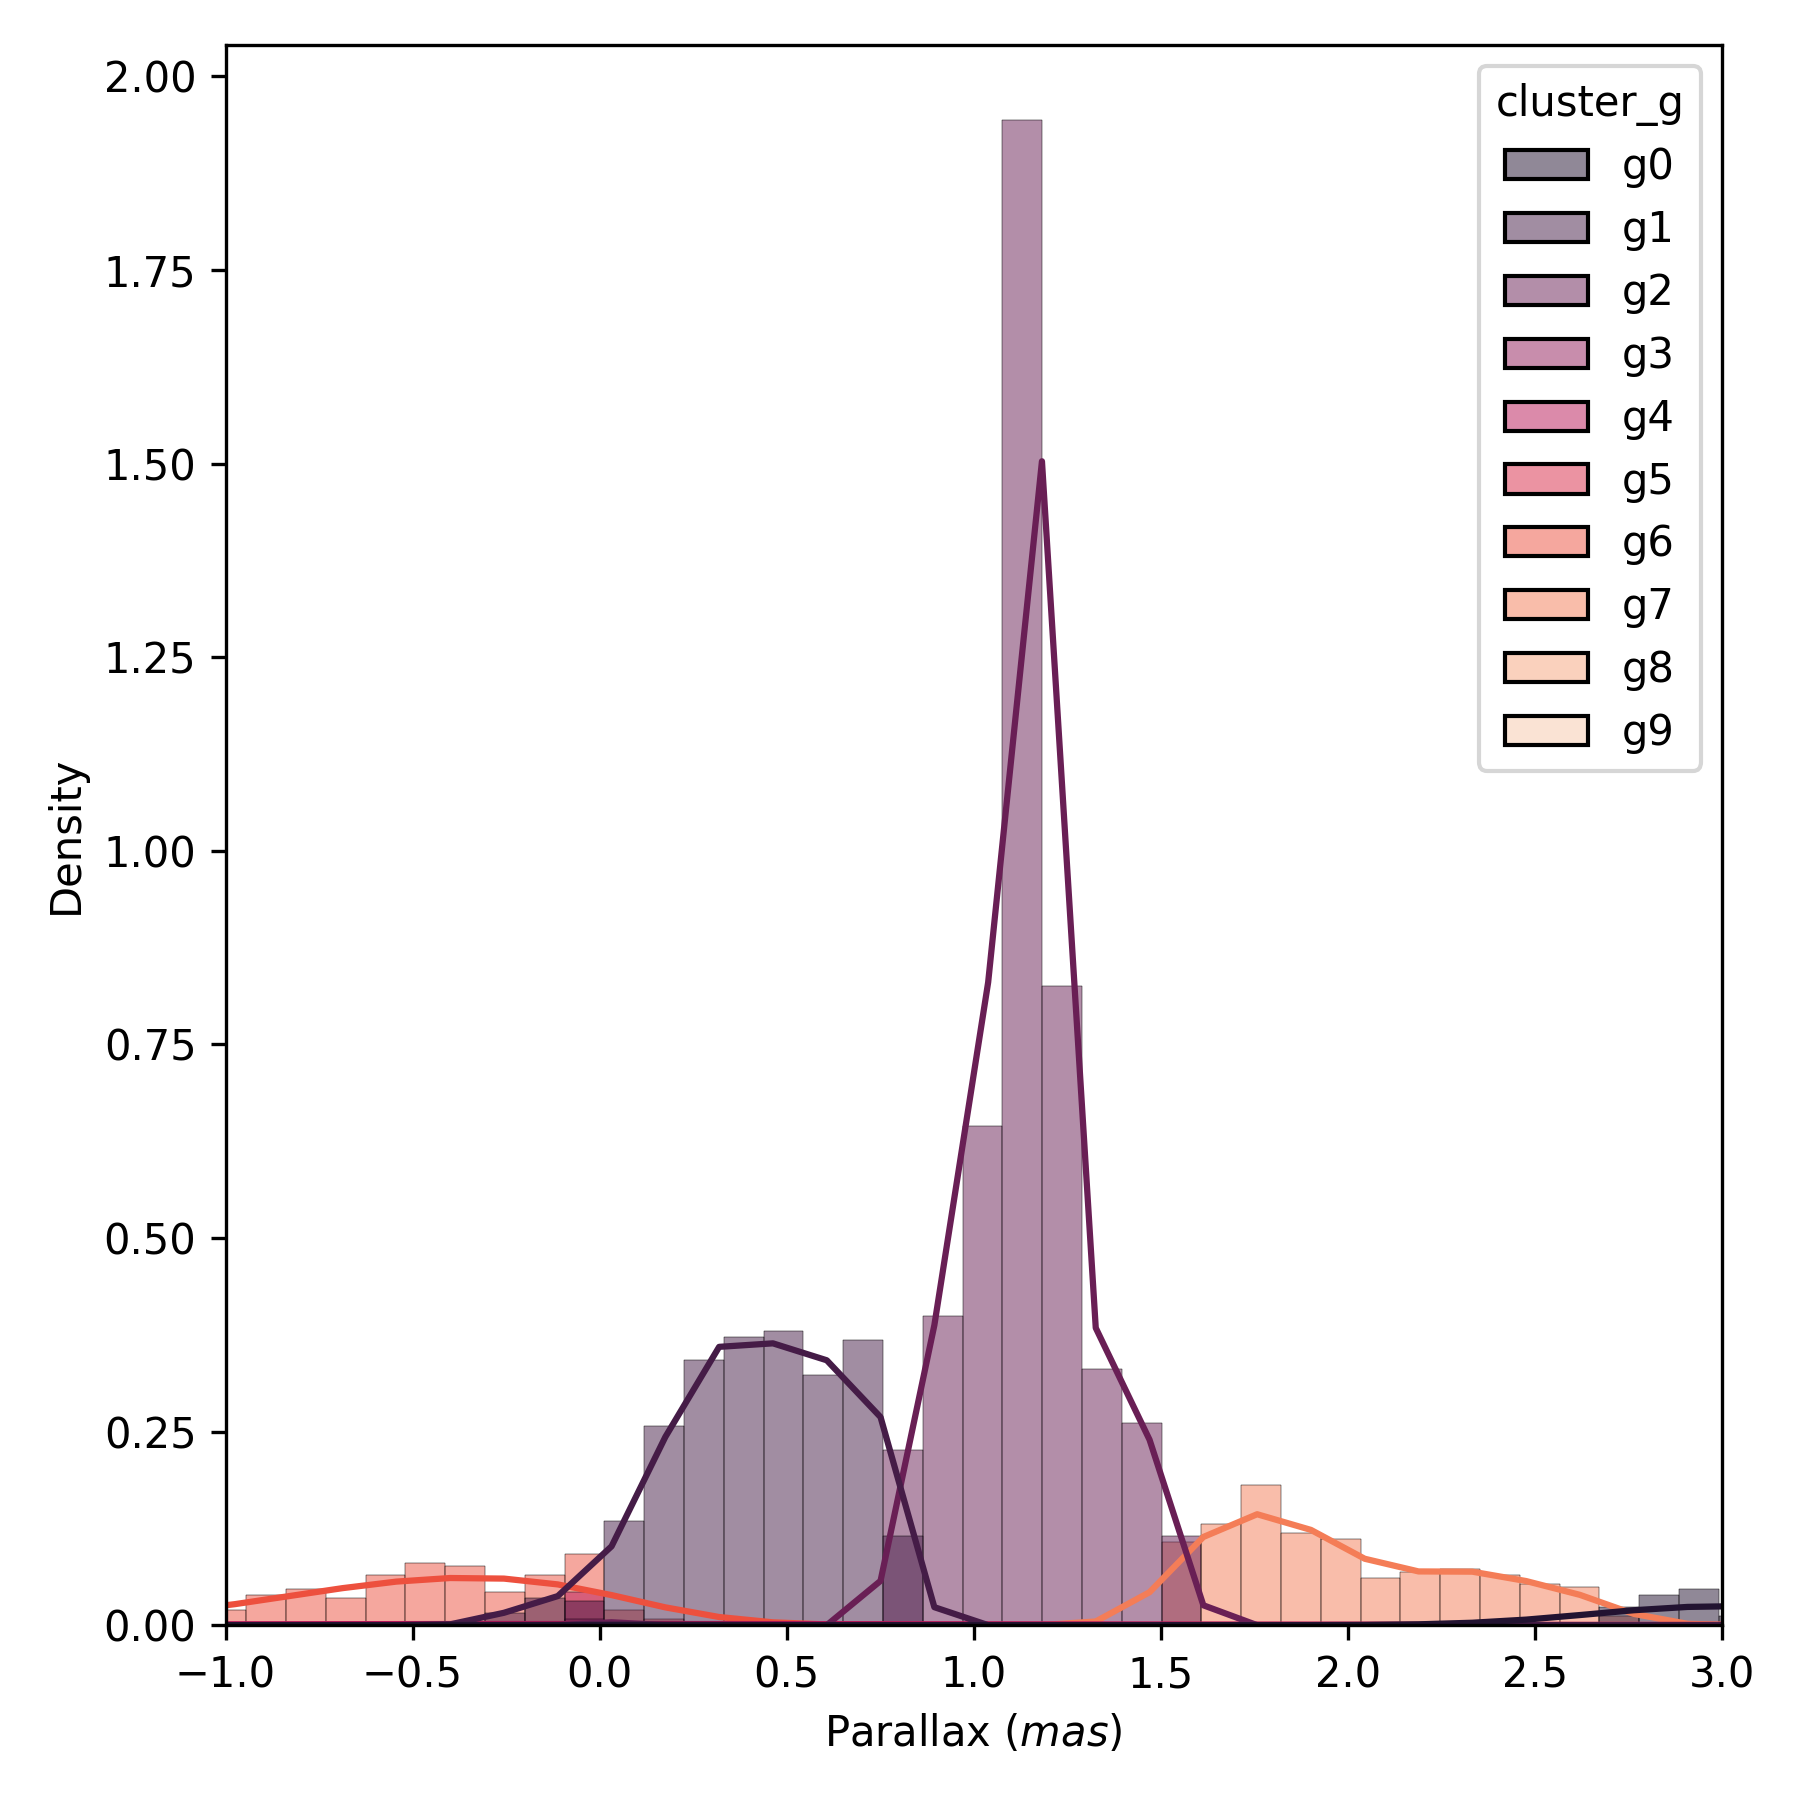
\includegraphics[width=\textwidth]{../figures/ngc_2682/dec_parallax_ngc_2682.png}
  \end{subfigure}
  \begin{subfigure}{0.29\textwidth}
    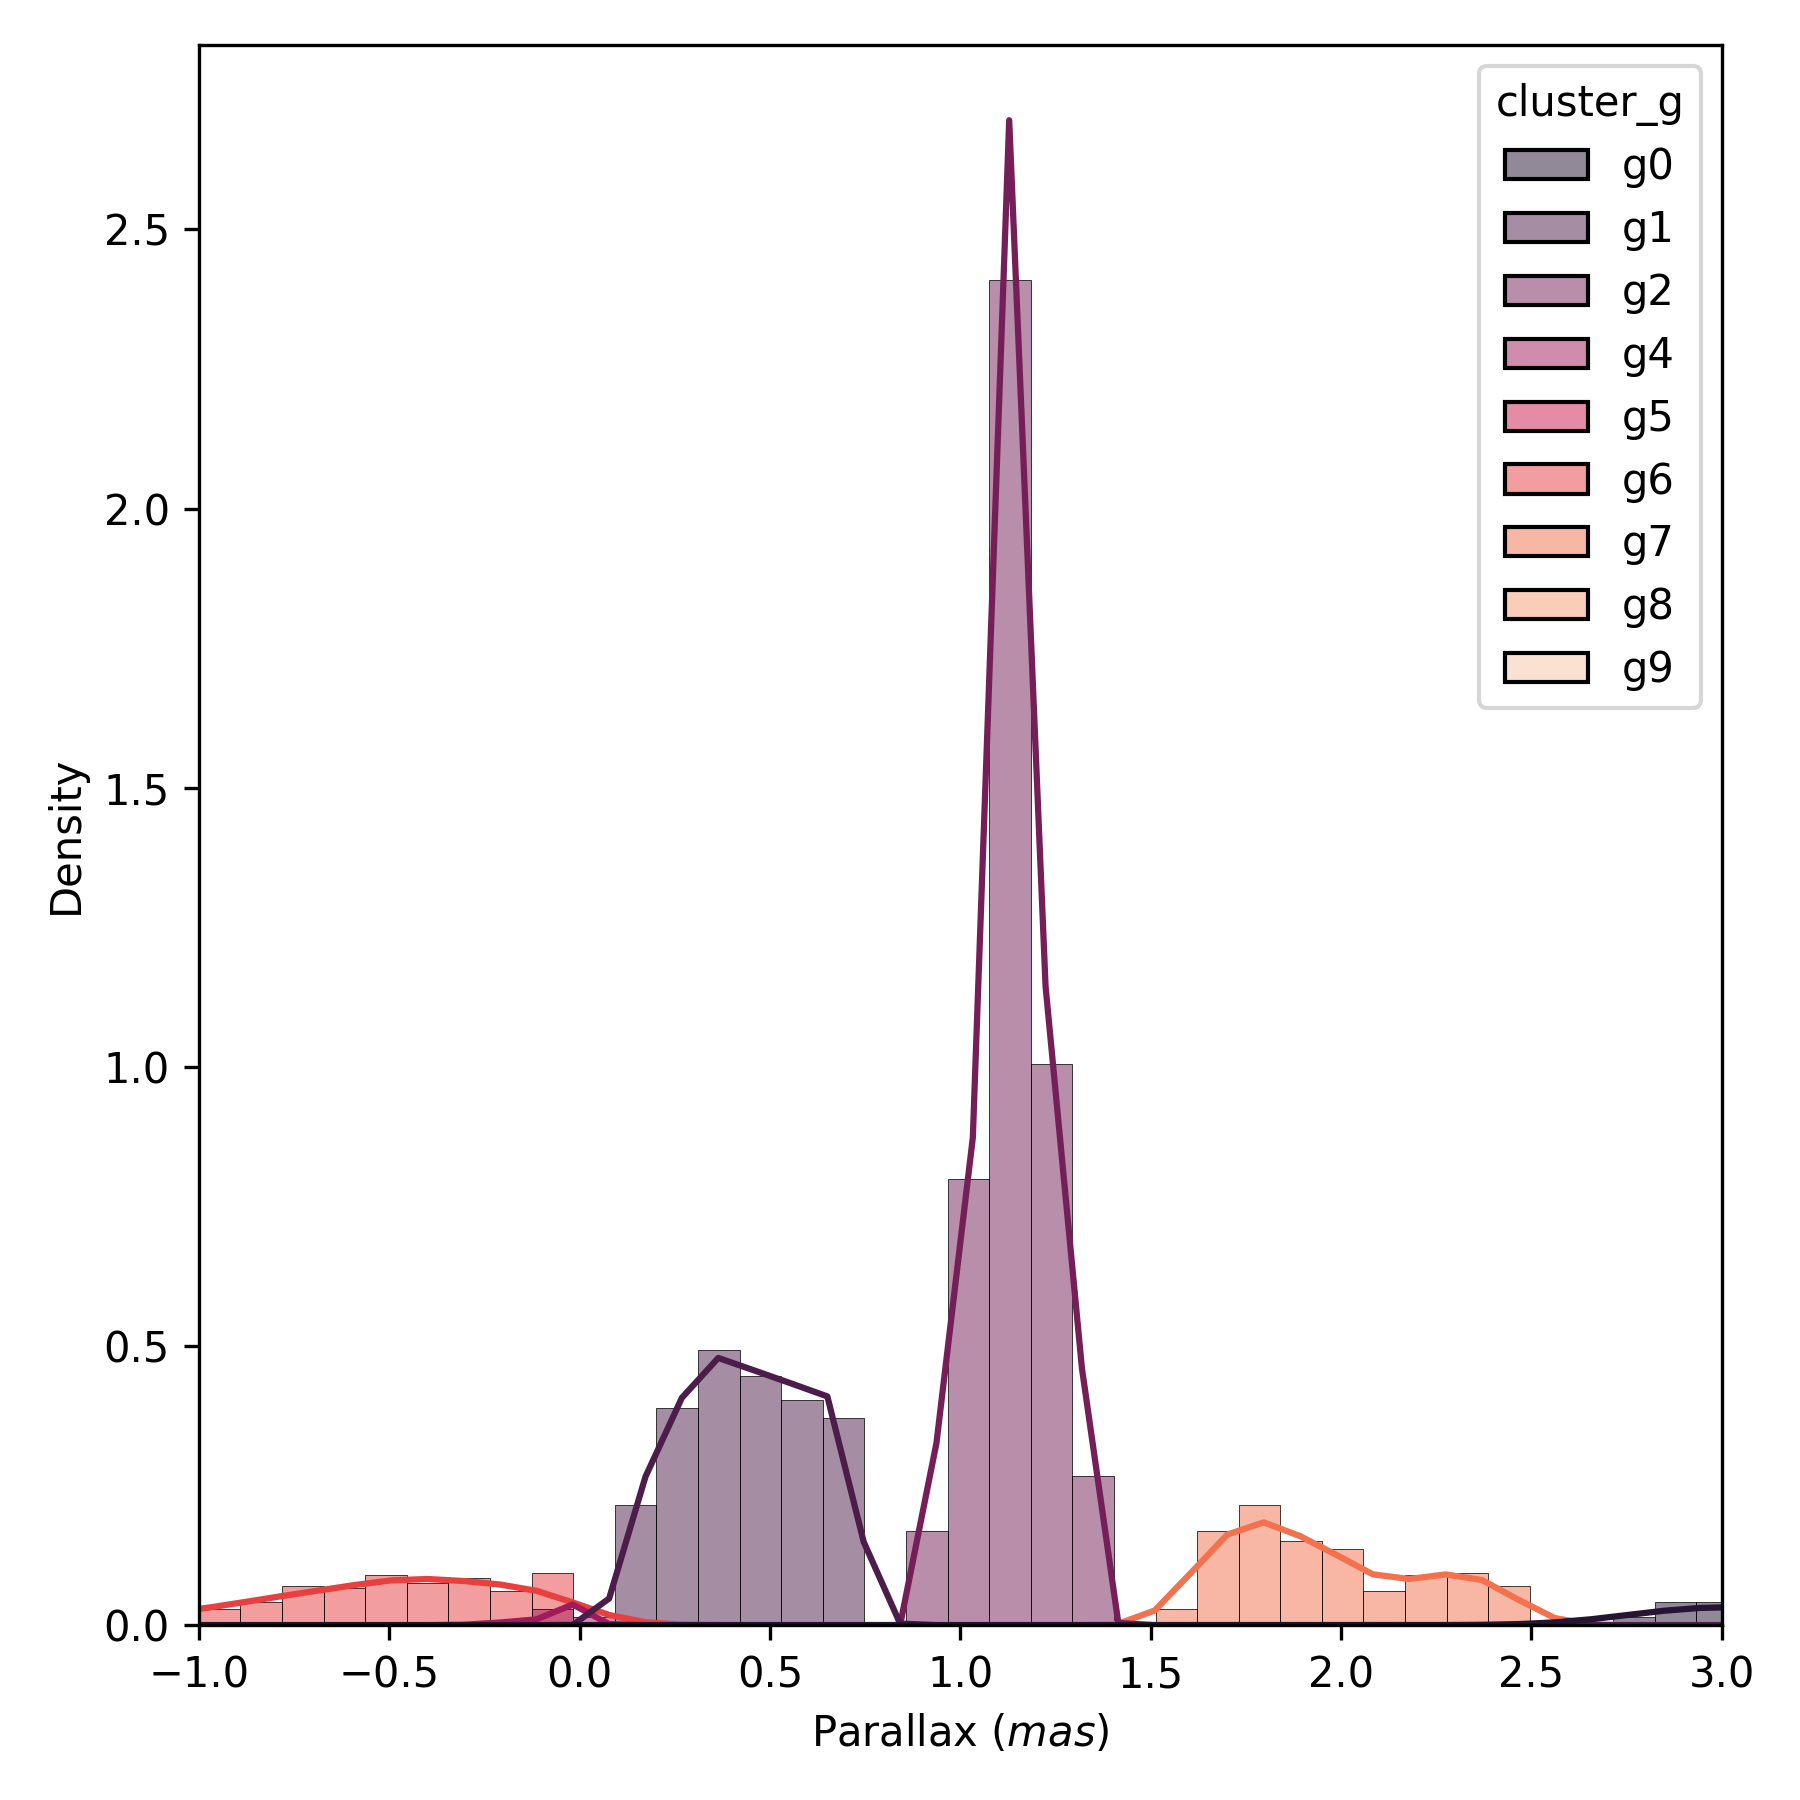
\includegraphics[width=\textwidth]{../figures/ngc_2682/dec_parallax_filtered_ngc_2682.png}
  \end{subfigure}

  \rotatebox[origin=c]{90}{{\bfseries } \strut}
  \rotatebox[origin=c]{90}{hr diagram\strut}
  \begin{subfigure}{0.29\textwidth}
    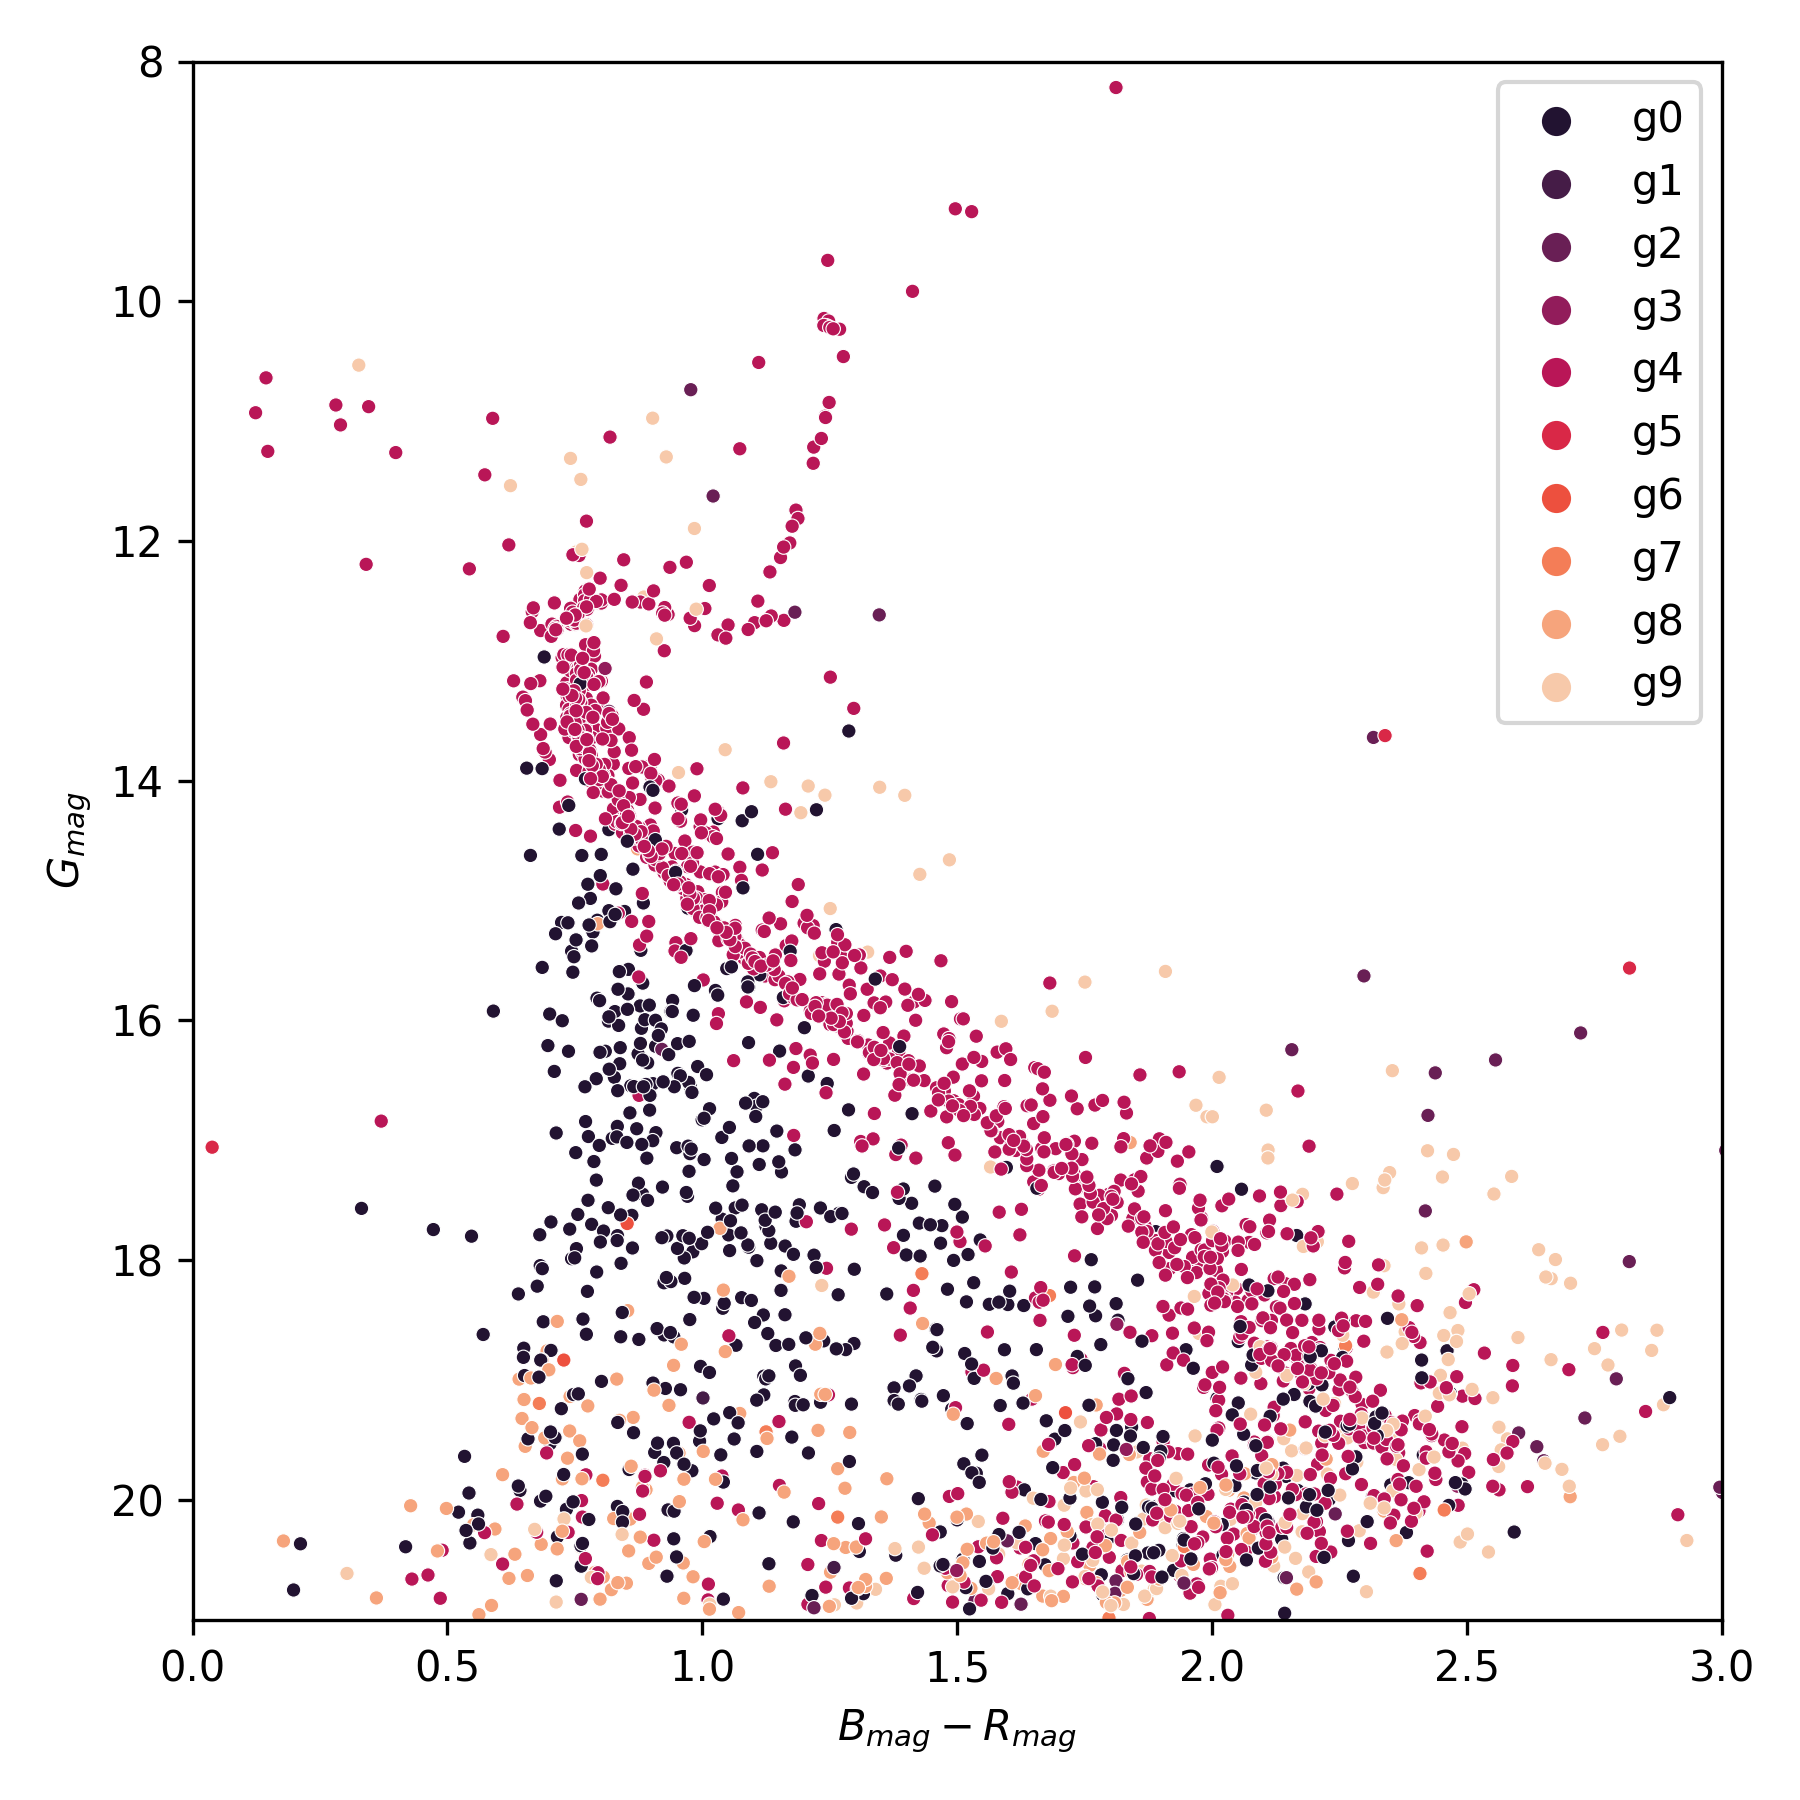
\includegraphics[width=\textwidth]{../figures/ngc_2682/kmeans_hr_diagram_ngc_2682.png}
  \end{subfigure}
  \begin{subfigure}{0.29\textwidth}
    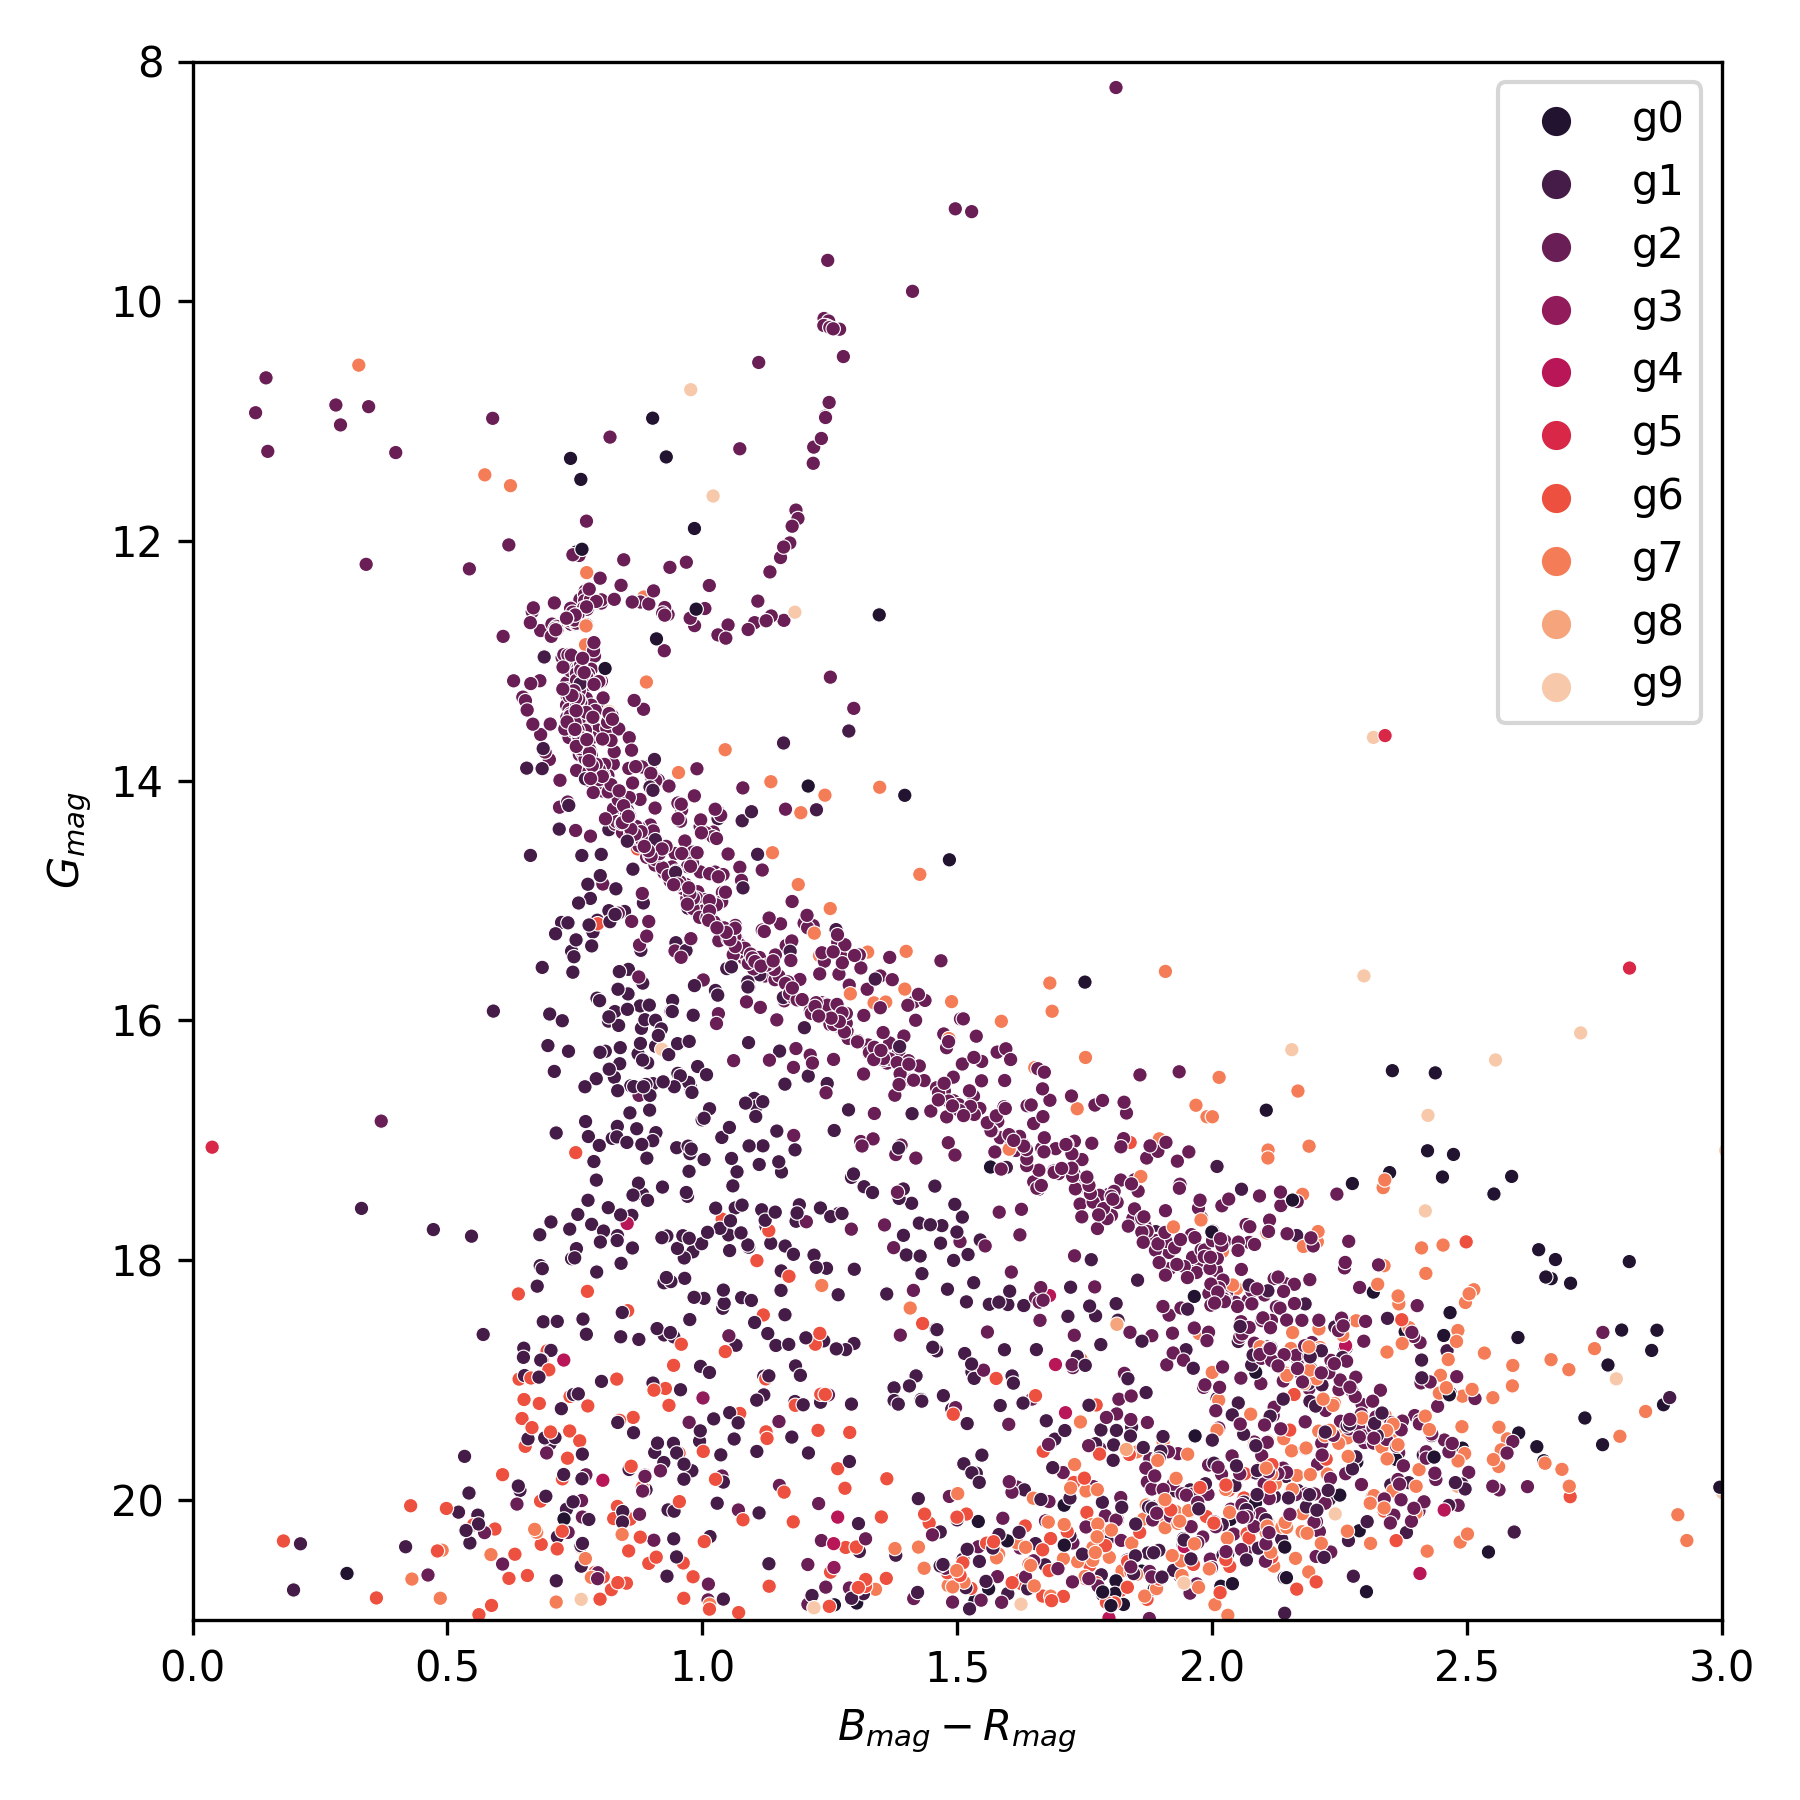
\includegraphics[width=\textwidth]{../figures/ngc_2682/dec_hr_diagram_ngc_2682.png}
  \end{subfigure}
  \begin{subfigure}{0.29\textwidth}
    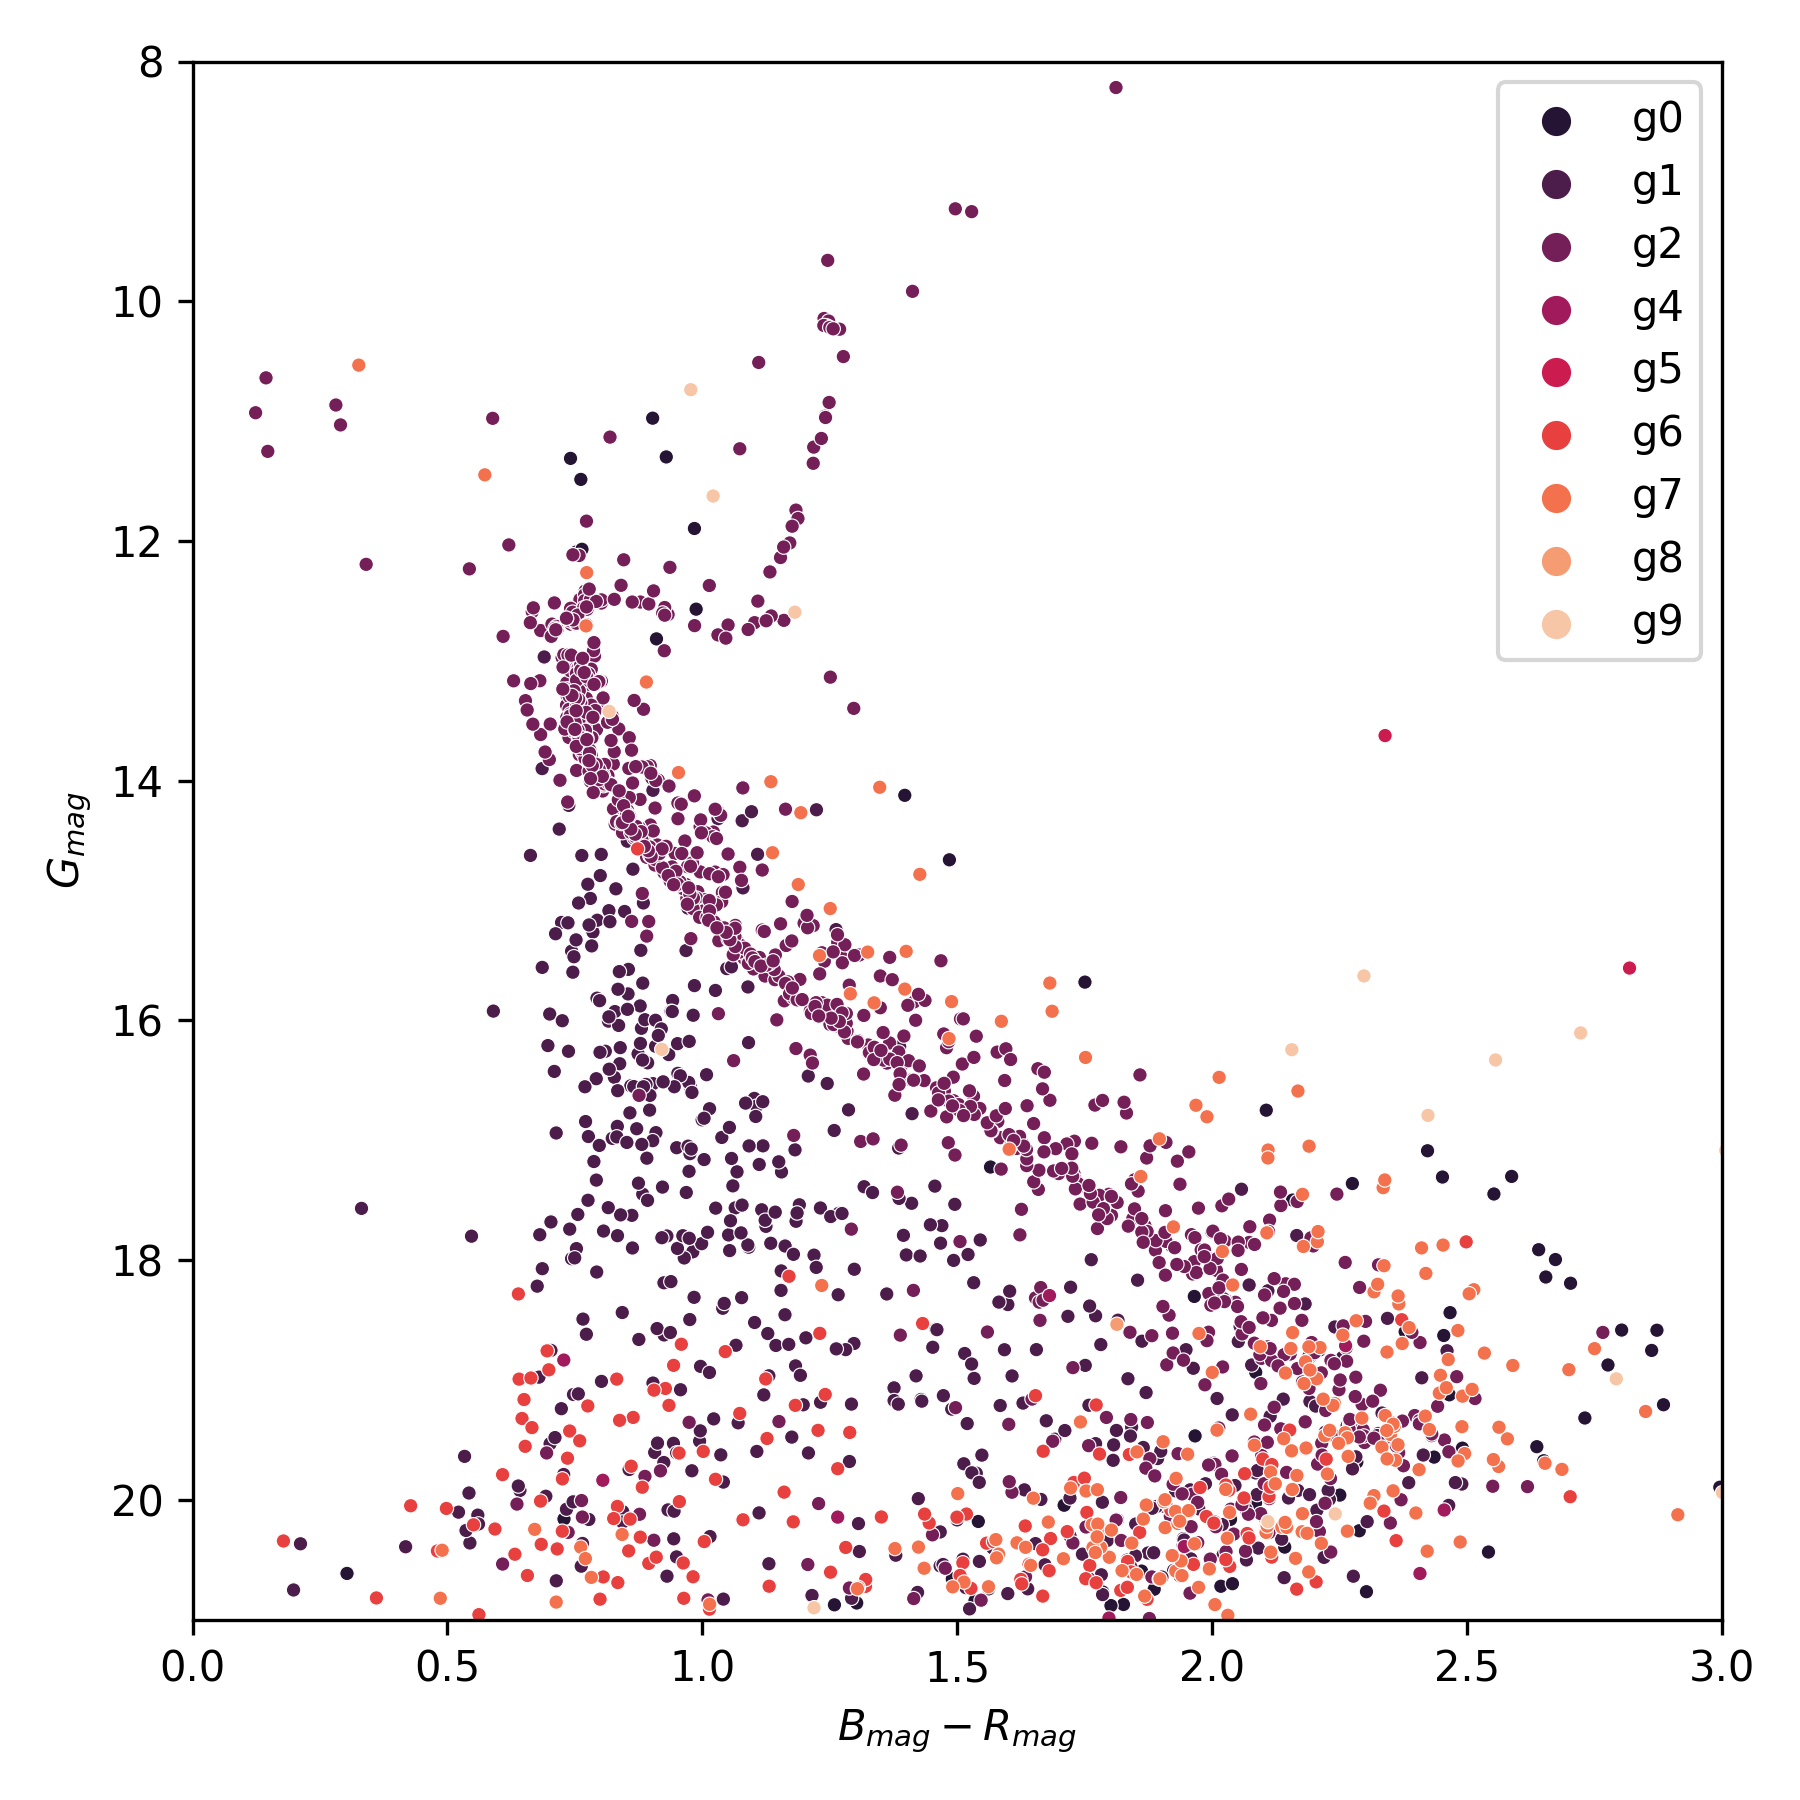
\includegraphics[width=\textwidth]{../figures/ngc_2682/dec_hr_diagram_filtered_ngc_2682.png}
  \end{subfigure}

  \rotatebox[origin=c]{90}{{\bfseries Melotte 22}\strut}
  \rotatebox[origin=c]{90}{parallax \strut}
  \begin{subfigure}{0.29\textwidth}
    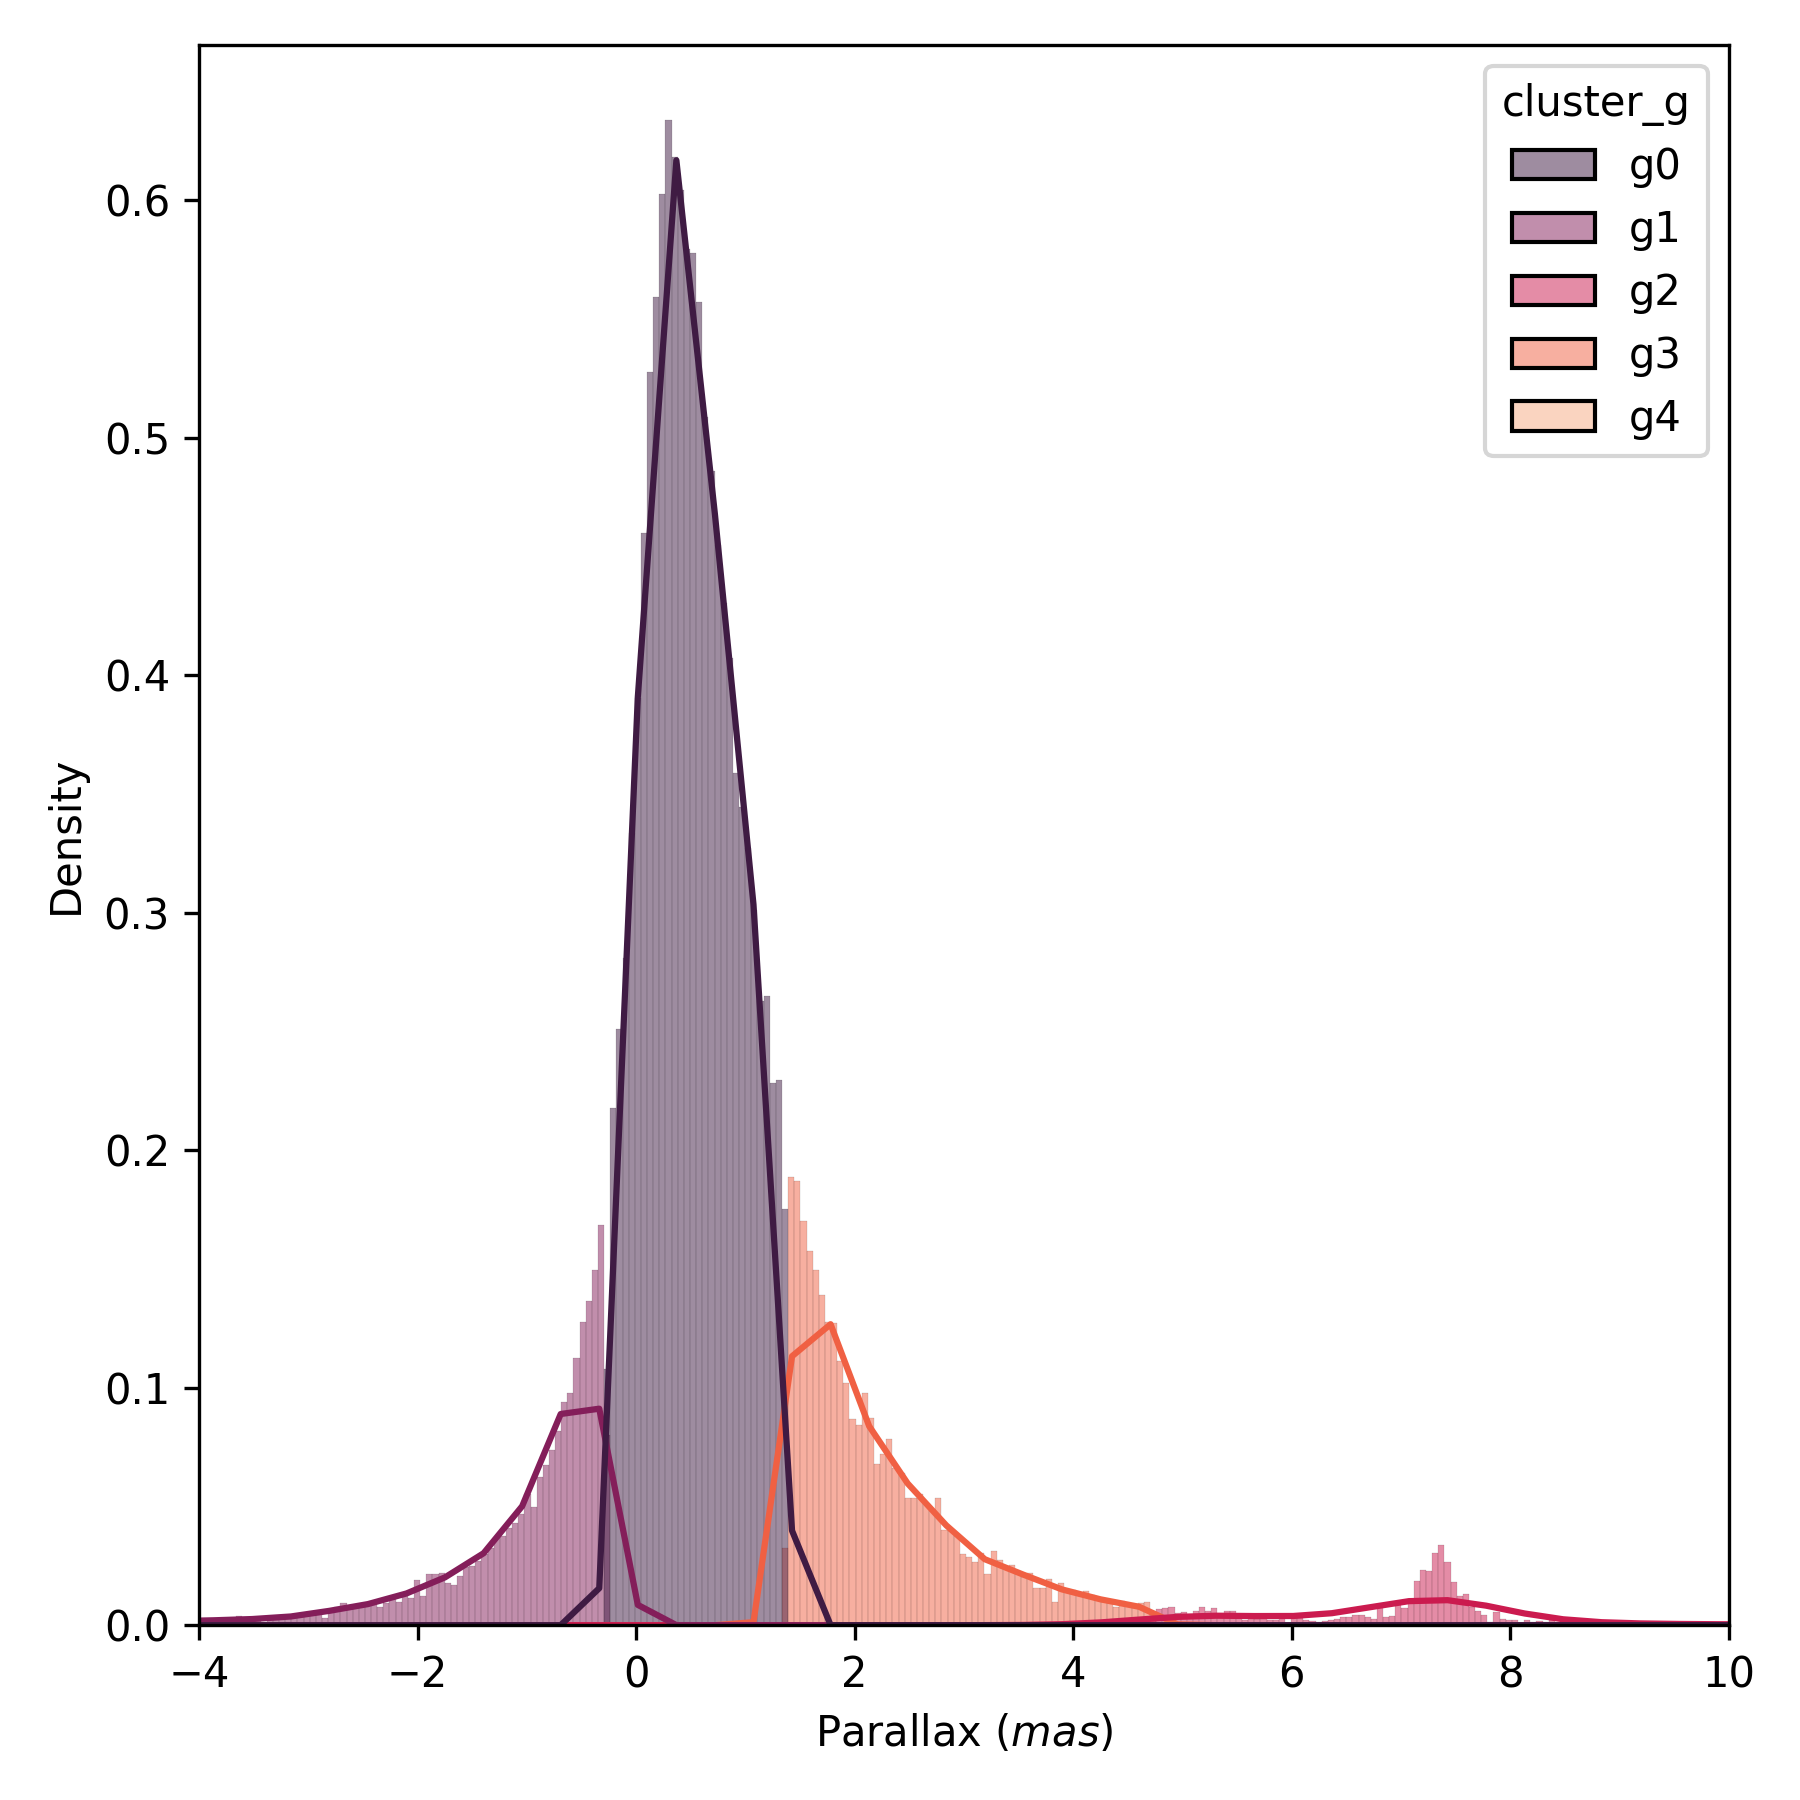
\includegraphics[width=\textwidth]{../figures/melotte_22/kmeans_parallax_melotte_22.png}
  \end{subfigure}
  \begin{subfigure}{0.29\textwidth}
    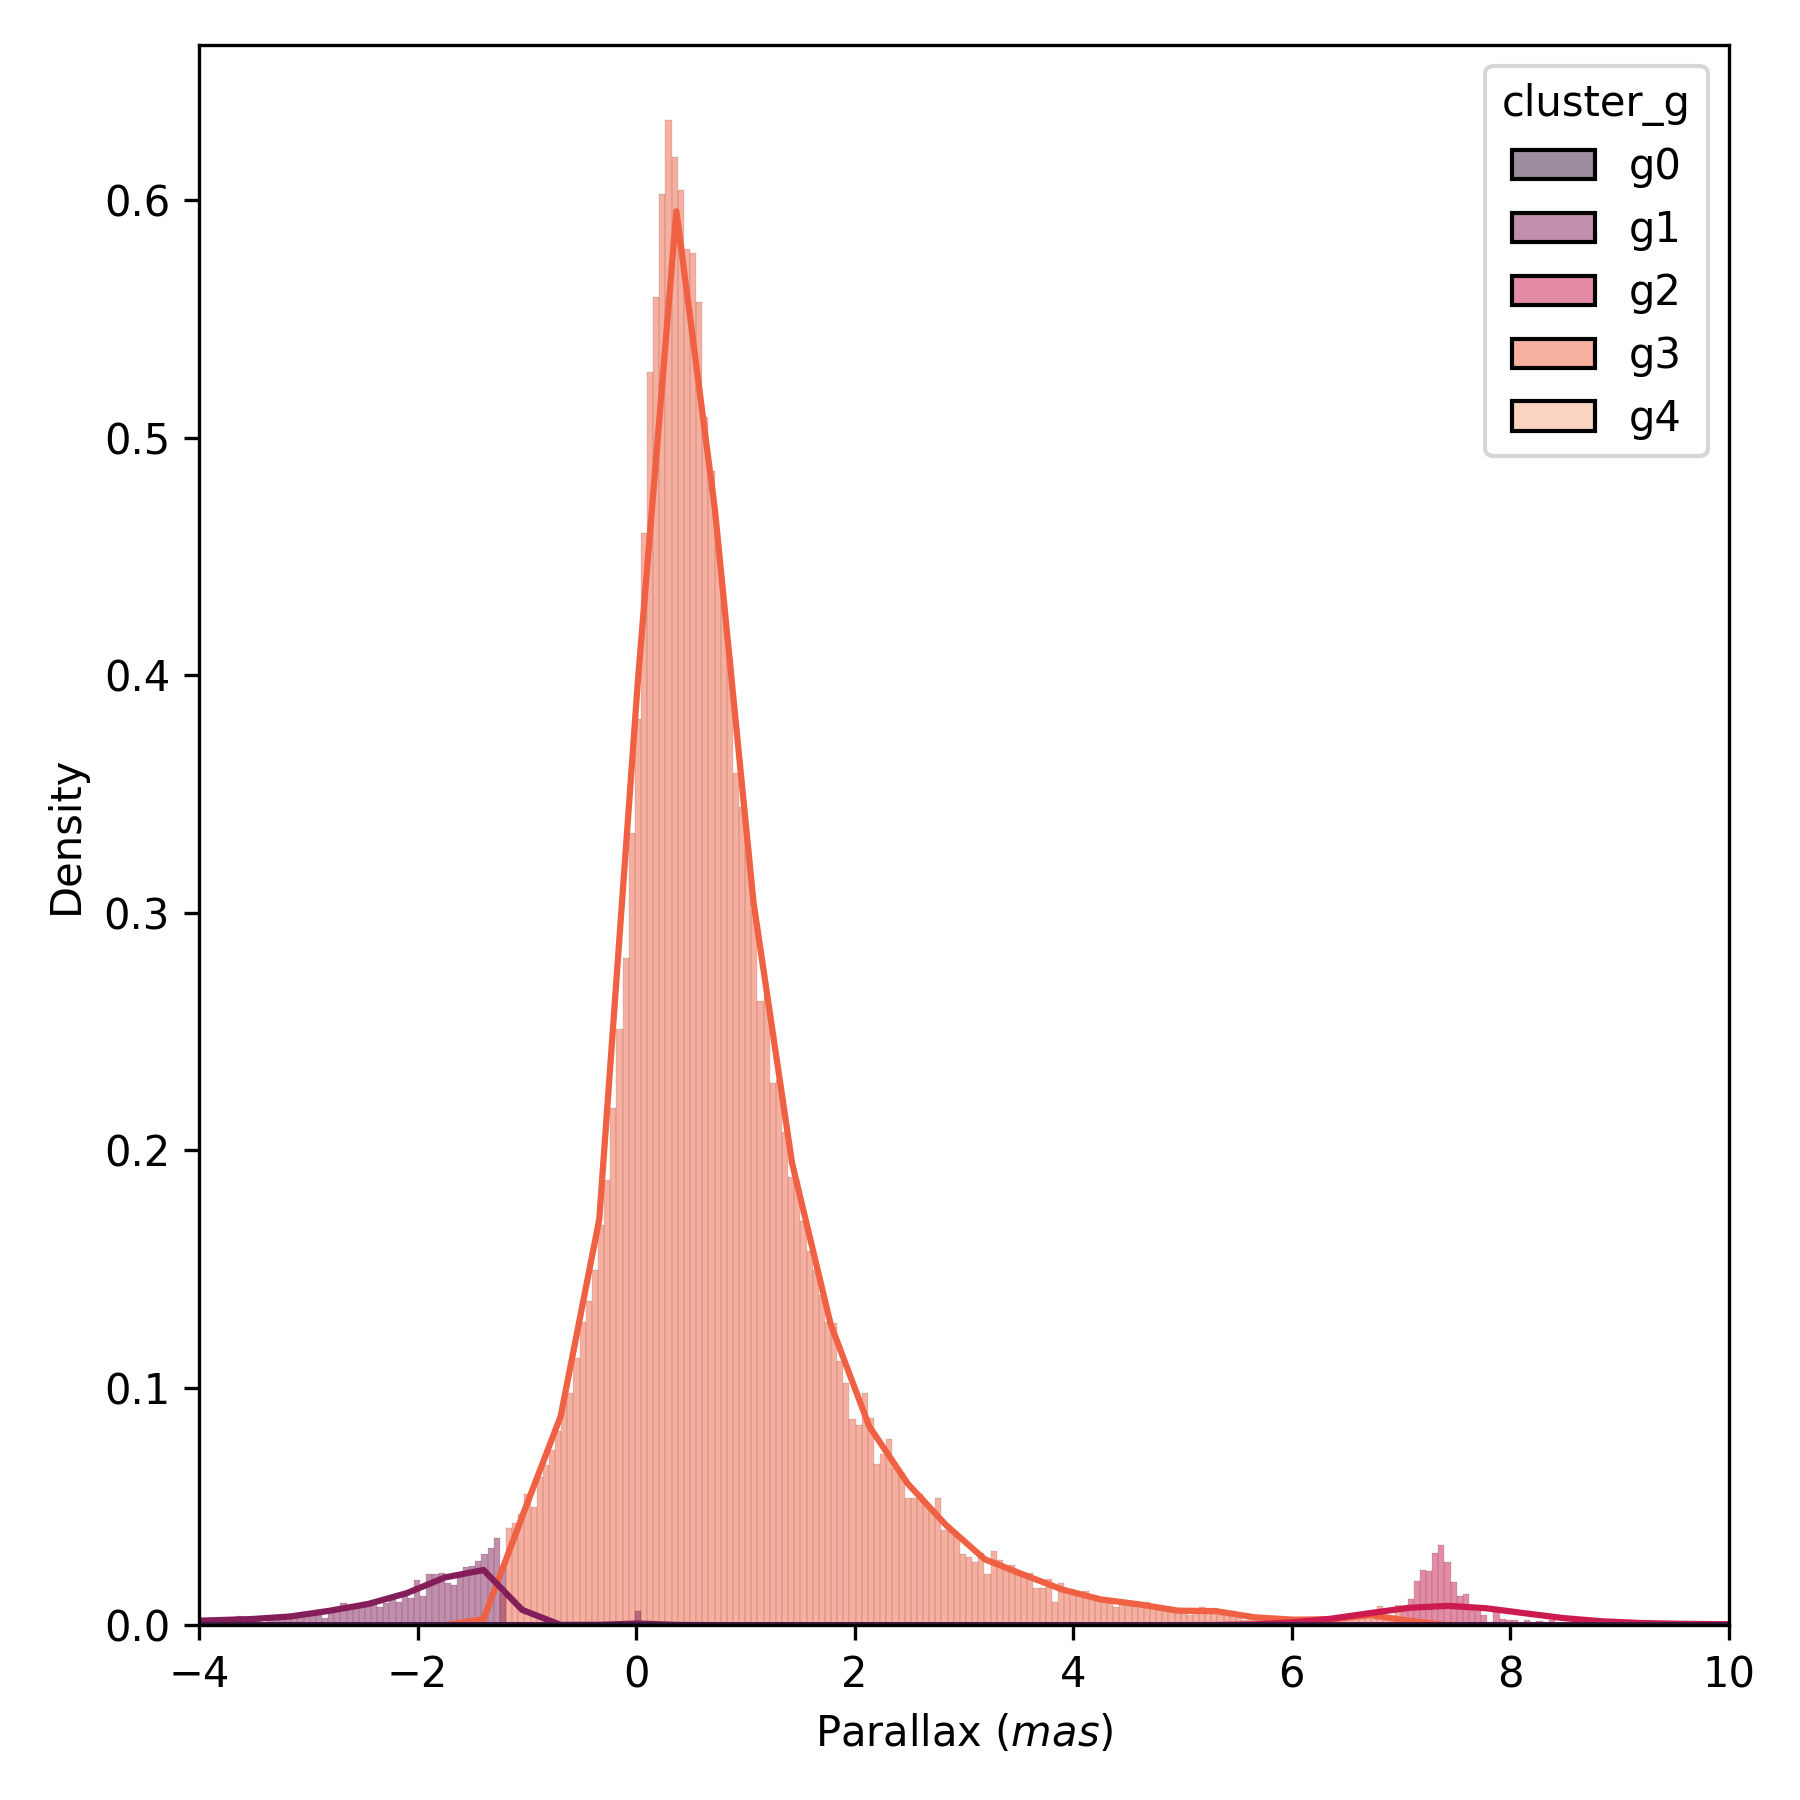
\includegraphics[width=\textwidth]{../figures/melotte_22/dec_parallax_melotte_22.png}
  \end{subfigure}
  \begin{subfigure}{0.29\textwidth}
    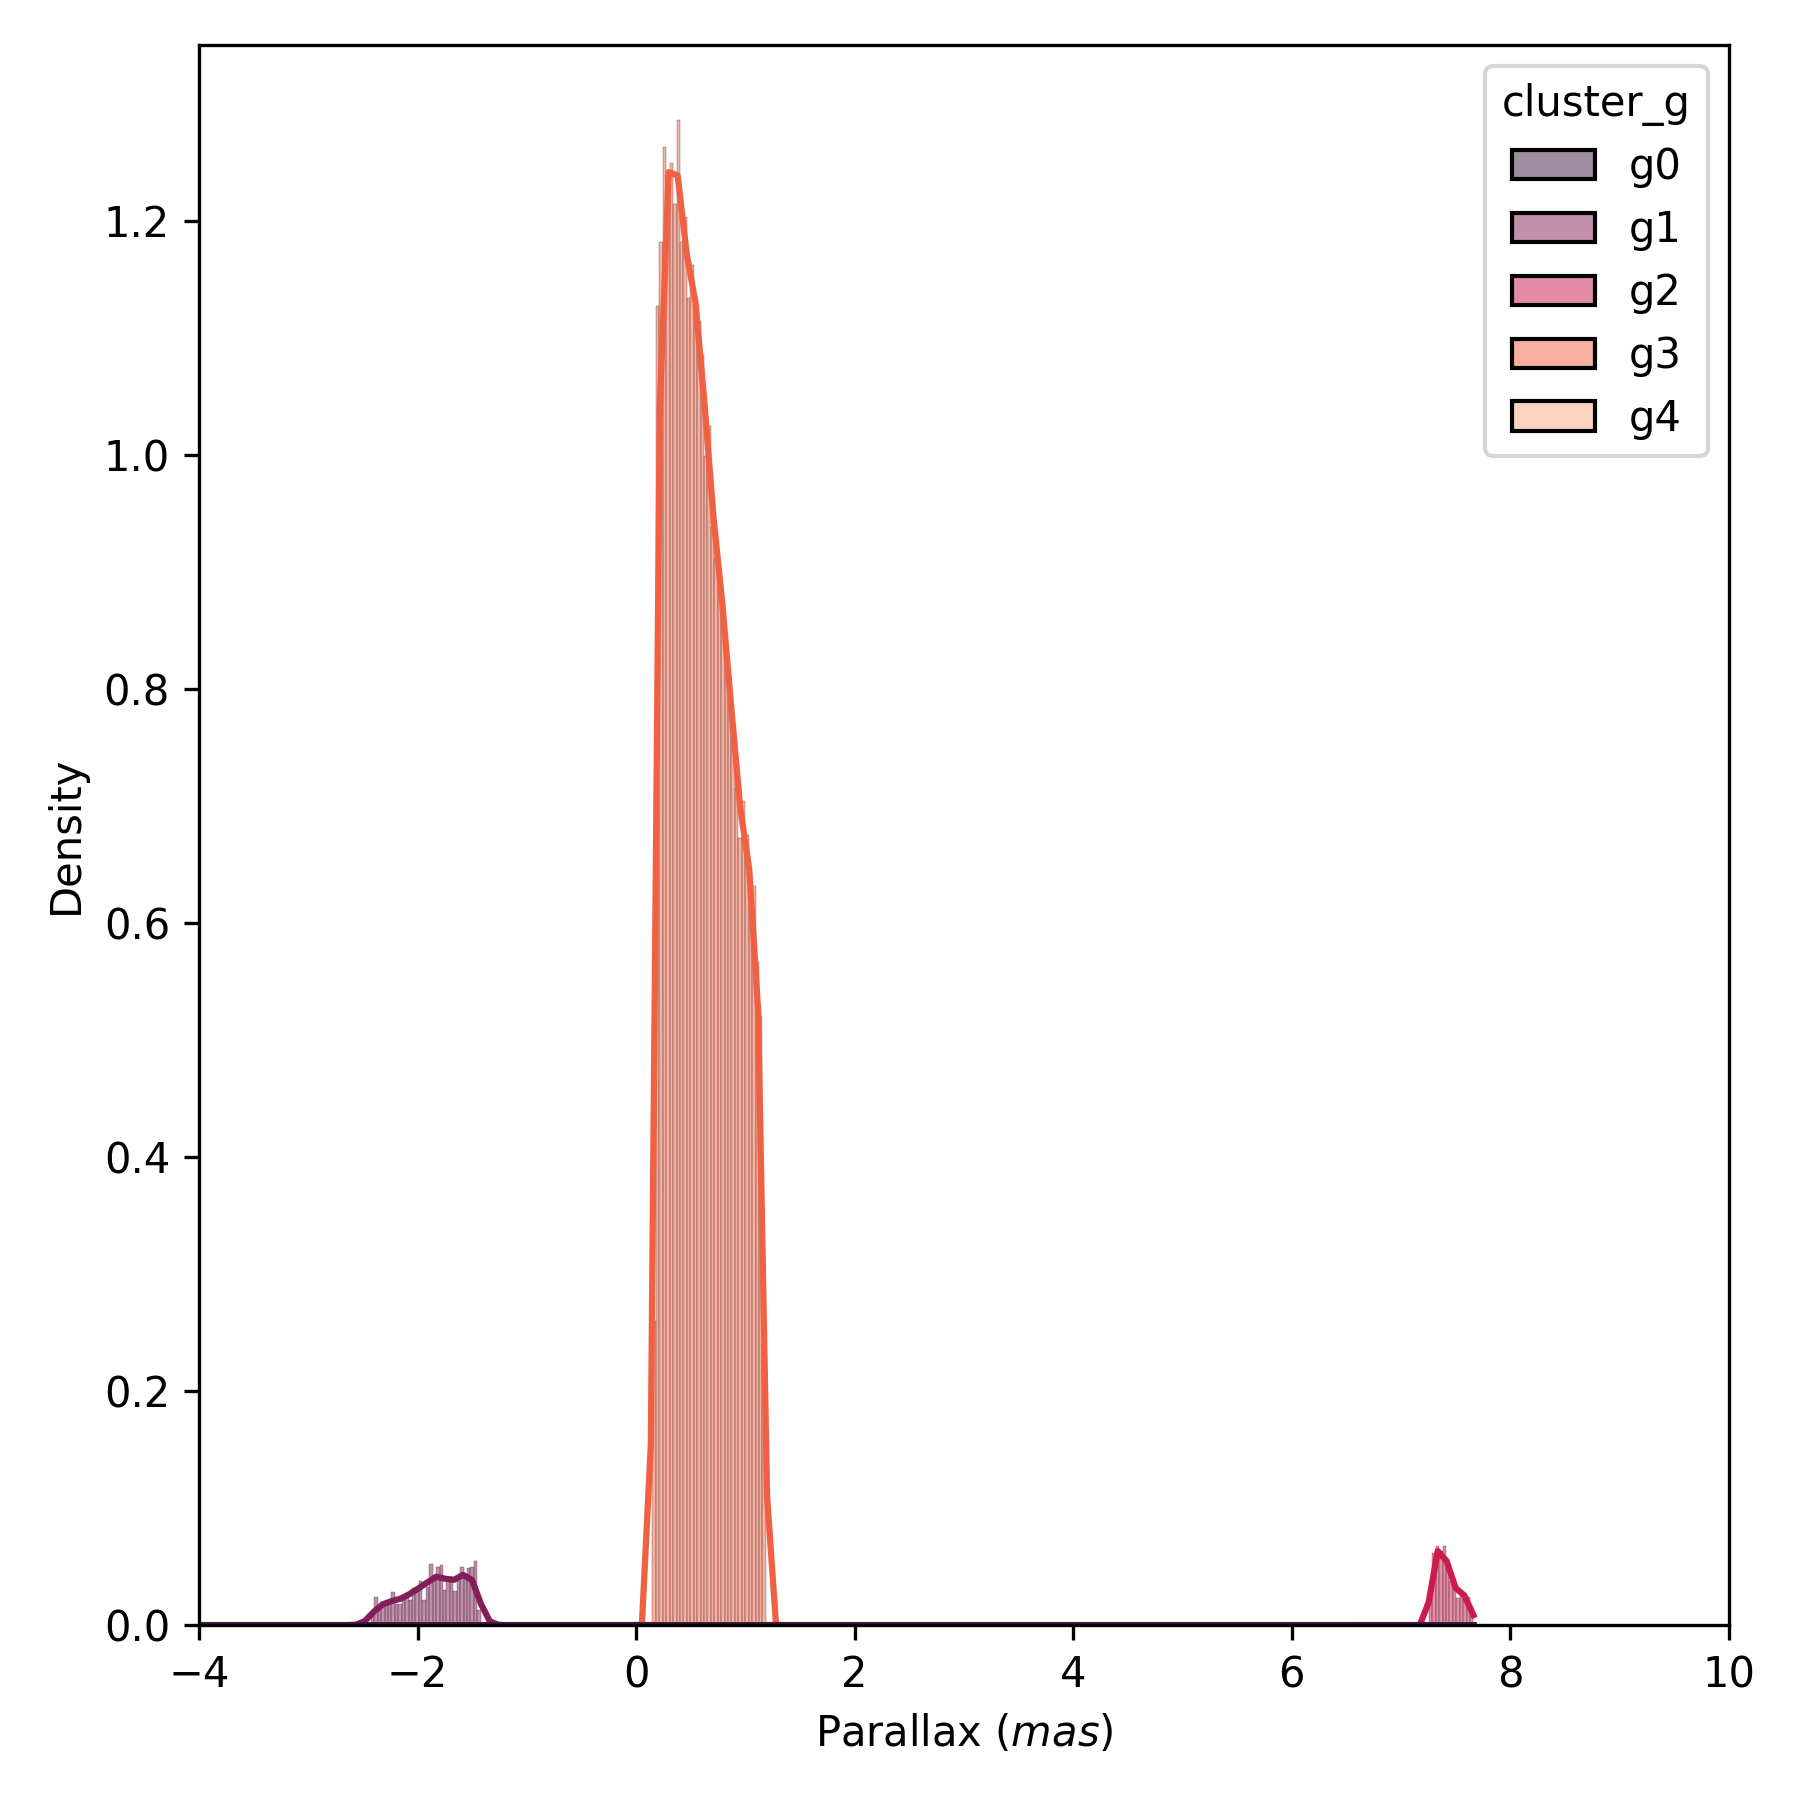
\includegraphics[width=\textwidth]{../figures/melotte_22/dec_parallax_filtered_melotte_22.png}
  \end{subfigure}

  \rotatebox[origin=c]{90}{{\bfseries } \strut}
  \rotatebox[origin=c]{90}{hr diagram\strut}
  \begin{subfigure}{0.29\textwidth}
    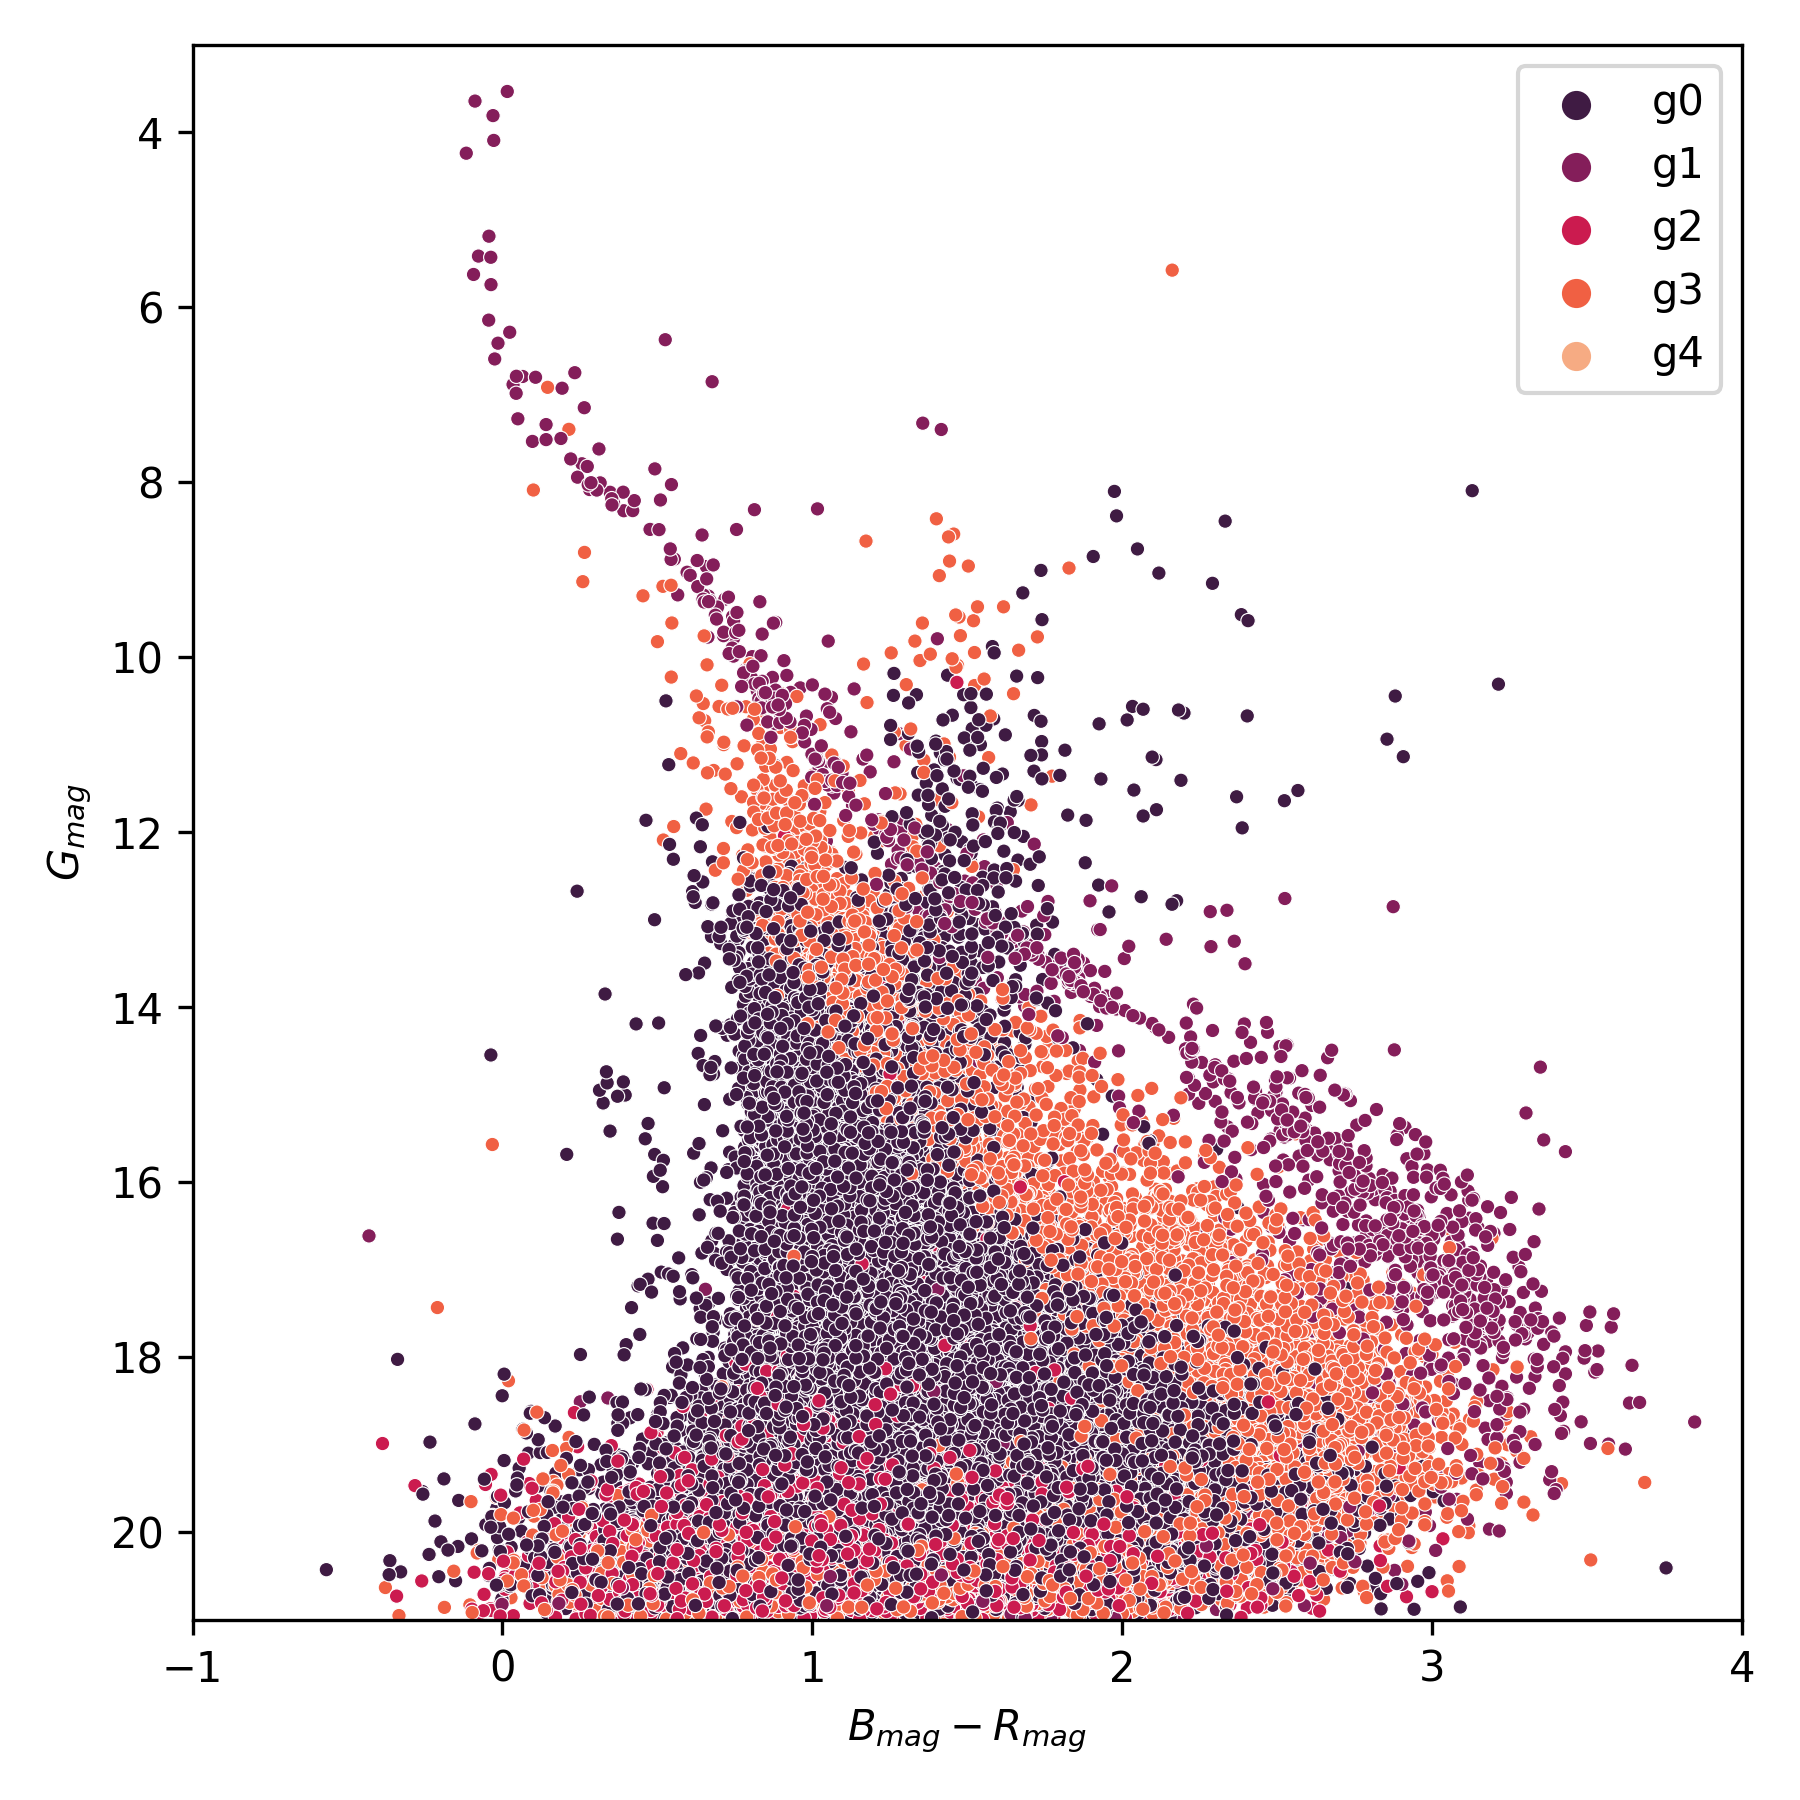
\includegraphics[width=\textwidth]{../figures/melotte_22/kmeans_hr_diagram_melotte_22.png}
    \caption{K-Means}
  \end{subfigure}
  \begin{subfigure}{0.29\textwidth}
    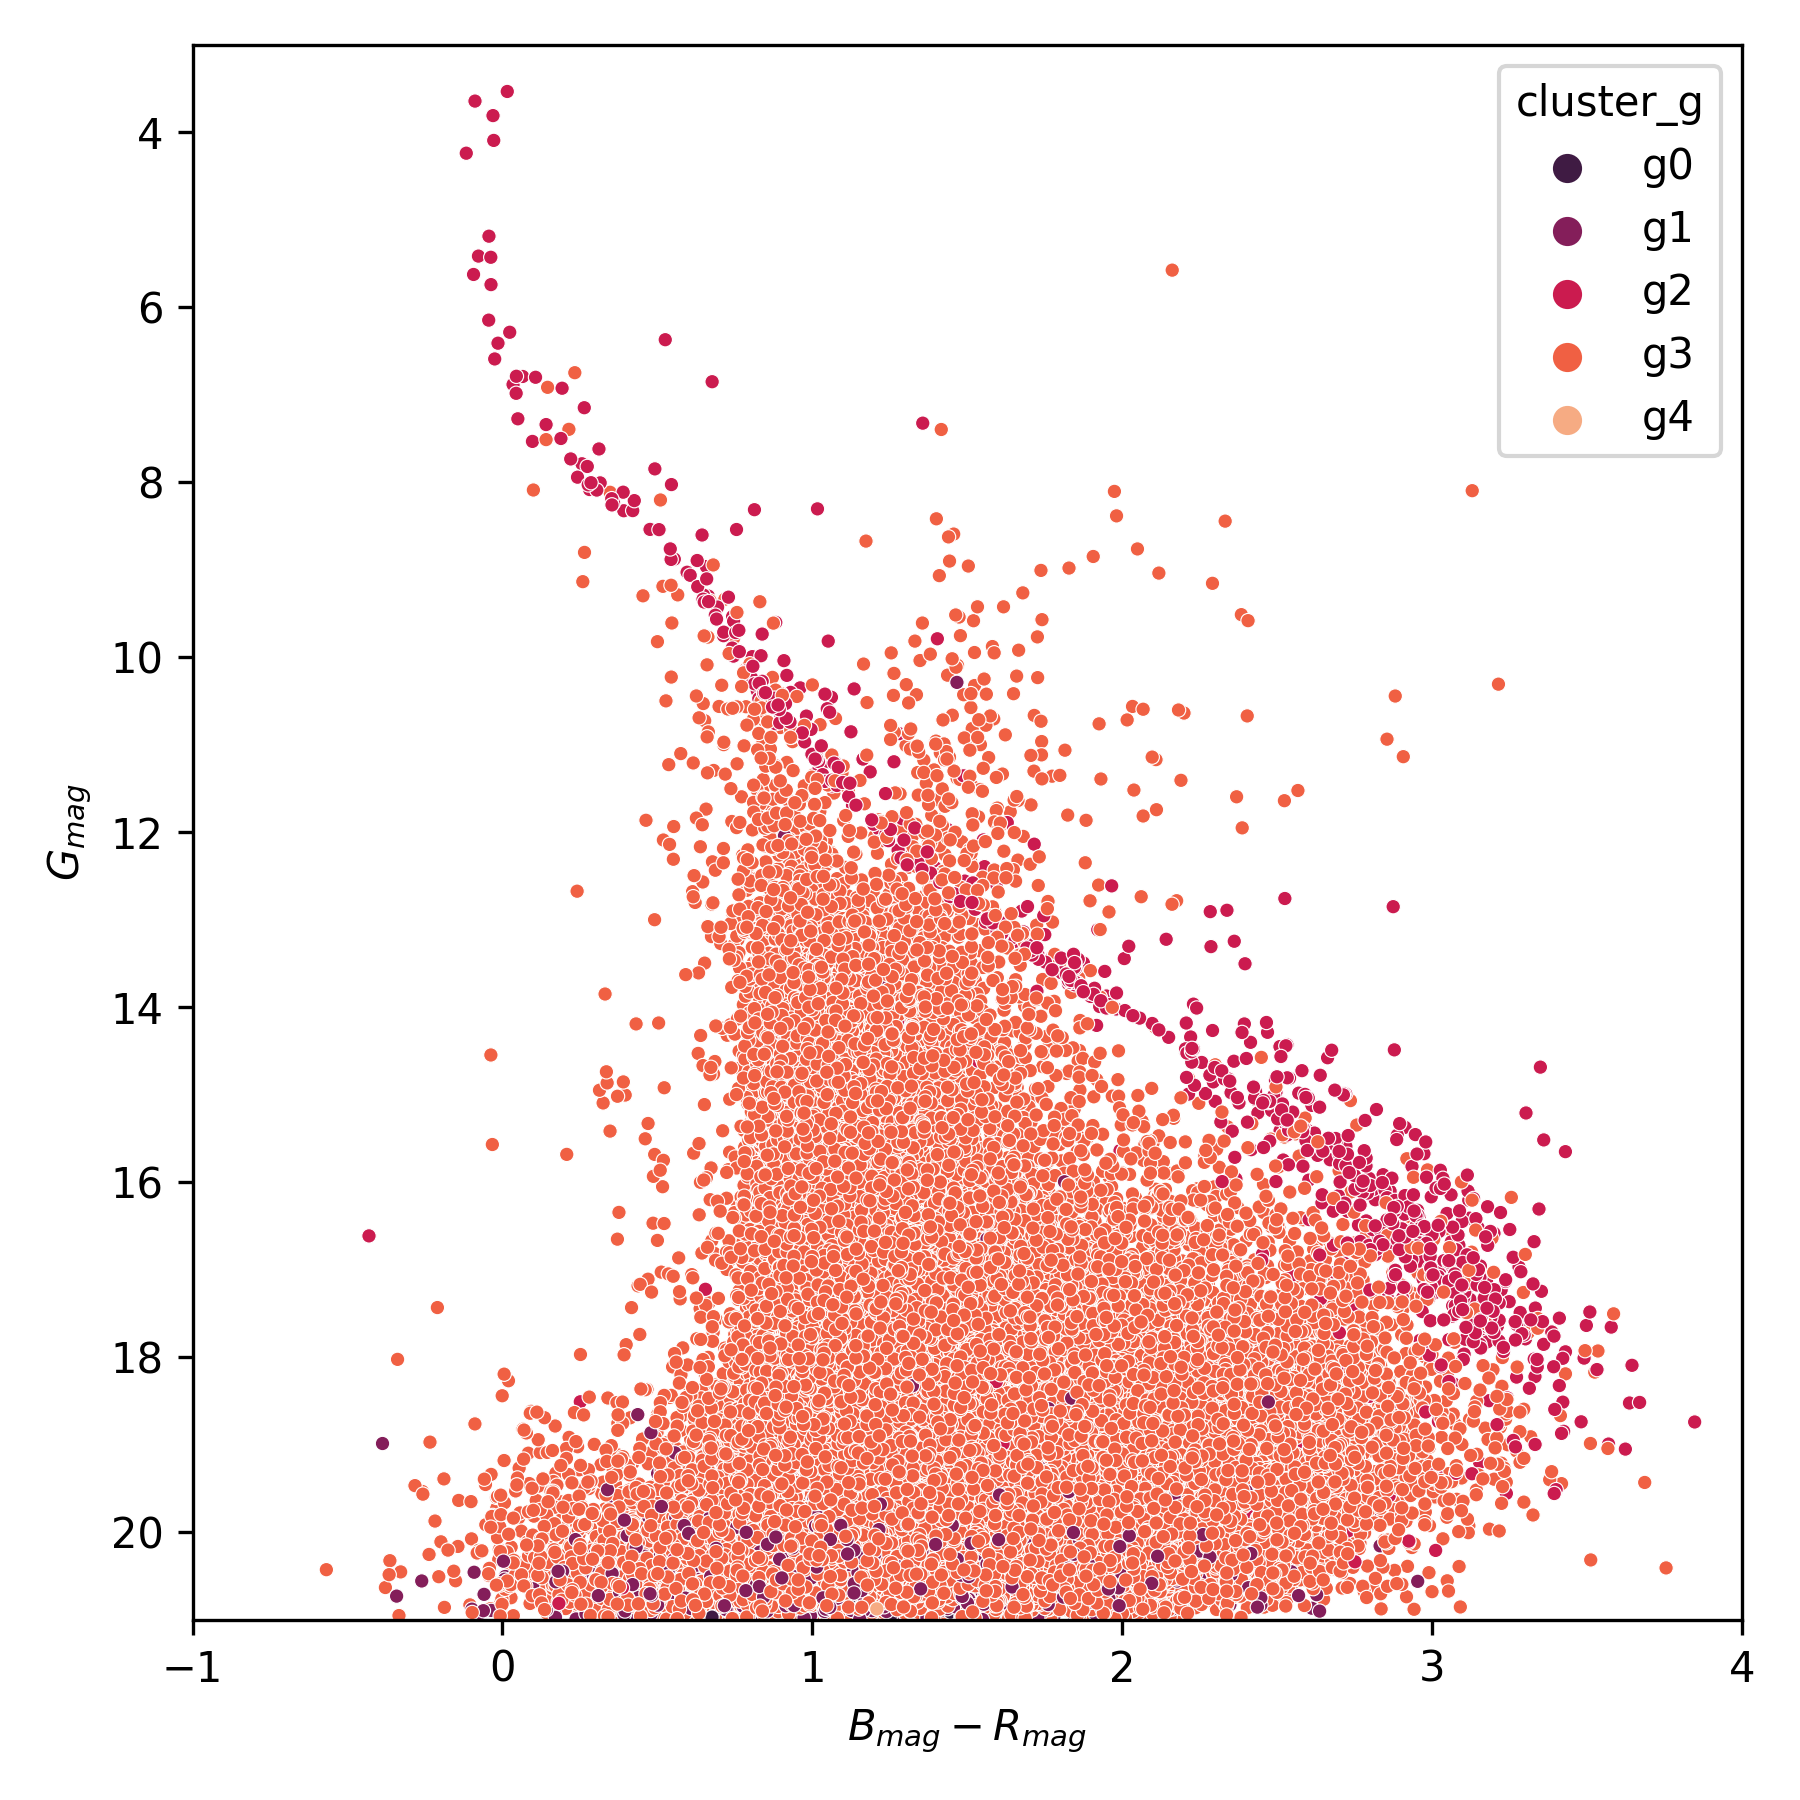
\includegraphics[width=\textwidth]{../figures/melotte_22/dec_hr_diagram_melotte_22.png}
    \caption{DECOCC}
  \end{subfigure}
  \begin{subfigure}{0.29\textwidth}
    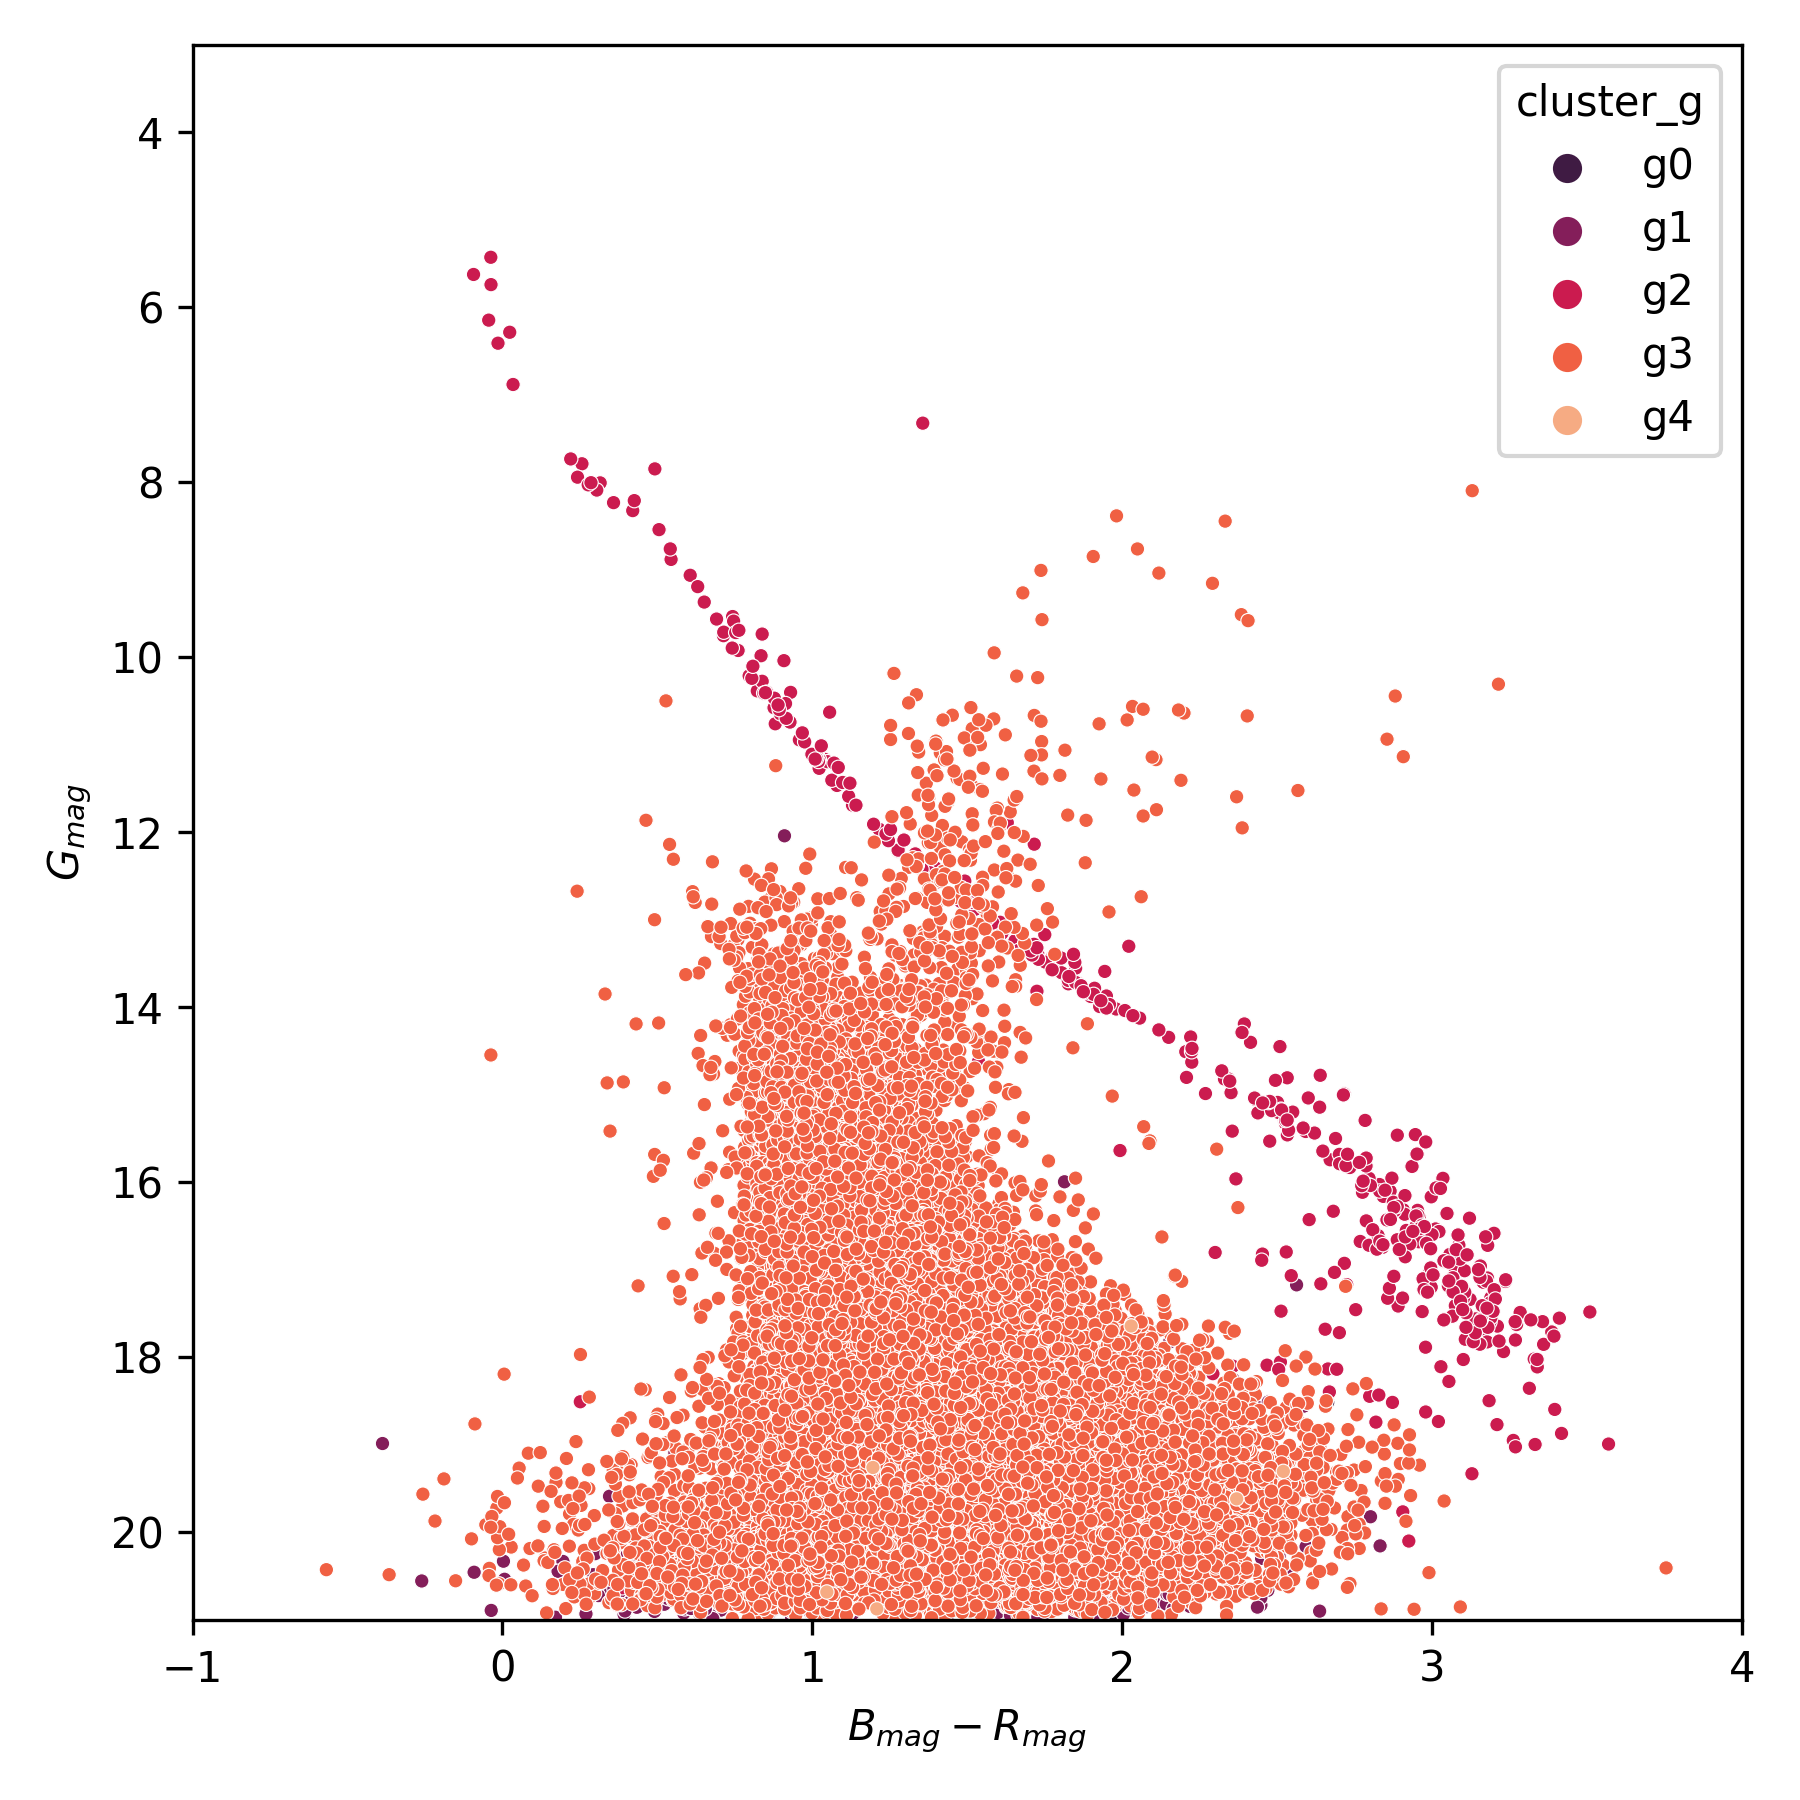
\includegraphics[width=\textwidth]{../figures/melotte_22/dec_hr_diagram_filtered_melotte_22.png}
    \caption{DECOCC (filt.)}
  \end{subfigure}
  \caption{Summary of the characterization for the clusters NGC 2682 and Melotte 22.}
  \label{fig:melotte_22_ngc_2682_characterization_evolution}
\end{figure*}

Figures~\ref{fig:ngc_2516_ngc_2632_characterization_evolution} (describes NGC 2516 and NGC 2632) and~\ref{fig:melotte_22_ngc_2682_characterization_evolution} (describes NGC 2682 and Melotte 22) show the groups found for the three models. For each open cluster, we describe the parallax and hr diagram.

In each open cluster, the models K-Means and DECOCC label the open cluster in the following groups:

\begin{itemize}
  \item NGC 2516: K-Means and our model label as \emph{g3}.
  \item NGC 2632: K-Means and our model label as \emph{g1}.
  \item NGC 2682: K-Means labels as \emph{g4}, and our model labels as \emph{g2}.
  \item Melotte 22: K-Means labels as \emph{g1}, and our model labels as \emph{g2}.
\end{itemize}

As we can observe, labels between K-Means and DECOCC do not match (except for NGC 2632), since we tested these two models independently. Thus, each model can label each group differently from the other. Moreover, running the same model twice can label the resulting groups differently between the first and the second run (as long as the same seed is not assigned). However, regardless whether the labels are different, the stars within the generated clusters should be very similar.

In all cases, the DECOCC model resolved properly the identity of the cluster and characterized the membership stars, giving compatible results with the ones obtained with classic procedures and VO tools~\cite{valdivielso2009iphas}.

Table~\ref{tab:app_hyperparameters_ngc_2516} describes the hyperparameters used for characterizing the open clusters with our method. Compared with the VO tools, we categorize our model as a non-parameterized model since it does not depend on parameters referred to as the cluster itself but only on hyperparameters such as the initial number of clusters to be found, or the structure of the Clustering Layer.

The proposed method is also non-supervised since we do not need to tell the model which stars belong to the cluster or assist it while its training stage.

Only at the end of the characterization, a fine-tuning driven by the user is applied to improve the selection by discarding those stars which fall outside the given quantiles. Nevertheless, we do not conceive assumptions about the cluster profile, something that we consider in VO tools. This is another evidence that our model is non-parameterized.

%% tabla comparativa de los hyperparametros
\begin{table}[htbp]
  \begin{center}

    % \resizebox{\columnwidth}{!}{
        \begin{tabular}{l|l|c}
          & \textbf{Hyperparameter} & \textbf{Value} \\
          \hline
          \multirow{4}{*}{\rotatebox[origin=c]{90}{NGC 2516}} & Number of Clusters & 8 \\
          & Clustering Layer & \(\left[ 50, 50, 60 \right]\) \\
          & Kernel Initializer Seed & 2 \\
          & Quantil Threshold & 0.15 \\\\

          % \caption{NGC 2632 DEC hyperparameters.}
          \multirow{4}{*}{\rotatebox[origin=c]{90}{NGC 2632}} & Number of Clusters & 10 \\
          & Clustering Layer & \(\left[ 50, 50, 40 \right]\) \\
          & Kernel Initializer Seed & 10 \\
          & Quantil Threshold & 0.1 \\\\


         % \caption{NGC 2682 DEC hyperparameters.}
          \multirow{4}{*}{\rotatebox[origin=c]{90}{NGC 2682}} & Number of Clusters & 10 \\
          & Clustering Layer & \(\left[ 50, 50, 40 \right]\) \\
          & Kernel Initializer Seed & 0 \\
          & Quantil Threshold & 0.1 \\\\

          % \caption{Melotte 22 DEC hyperparameters.}
          \multirow{4}{*}{\rotatebox[origin=c]{90}{Melotte 22}} & Number of Clusters & 5 \\
          & Clustering Layer & \(\left[ 50, 50, 200 \right]\) \\
          & Kernel Initializer Seed & 11 \\
          & Quantil Threshold & 0.1 \\

        \end{tabular}
    % }
    \caption{Hyperparameters of DECOCC model for the open clusters with different typologies.}
    \label{tab:app_hyperparameters_ngc_2516}
  \end{center}
\end{table}

In summary, we can say that our results improve K-Means. We based this judgment by comparing right ascension, declination, parallax, and the number of stars of the cluster found by the two models with the Simbad database. In other words, we statistically analyze the results not individualized by stars belonging to the cluster found. We arrange it with Simbad because as far as we are concerned, there is no Gaia dataset with classified open clusters.

\section{Conclusions}

This paper presents a model to characterize open clusters, comprising an Artificial Neural Network, which is neither parameterized nor supervised. The model does not require complex hardware. Instead, it can be run on workstations with a common GPU, making it accessible for deployment in many research centers.

The model works well in identifying and characterizing open clusters. However, some improvements must be made to improve its accuracy and precision.

The number of hyperparameters in our model is small and we do not need previous knowledge about the cluster studied, which makes it easier to test different settings and automate the process.

Building a non-parameterized model is a difficult and sometimes and unfeasible task due to every machine learning model requires initial definitions of the hyperparameters to work properly. However, in our model, the user is not required to provide any information about the cluster profile or its properties. Making it a non-parameterized model. Nevertheless, some tweaks can be done regarding the cluster and the studied region, like changing the initial number of clusters or modifying the clustering layer structure to improve the final characterization.

The initializer kernel prepares data before passing them to the ANN. This is one of the reasons because the results may vary significantly. In future works, we want to avoid it to have a reliable model which does not depend on the dataset order.

In future, we also want to test our model with a wider range of clusters. In general, we could think of applying it to the entire VizieR catalog. So, we could get a better idea about the current limitations of our model and improve it. For instance, we could determine with higher accuracy the typologies that our model works well with. Furthermore, we could establish different sets of hyperparameters regarding the typology of the cluster.

An important aspect we noticed is that with our model new uncatalogued clusters arise from the data apart of the main ones. Making it of special interest to study these individual new clusters.

Another possible improvements are either to use DBSCAN instead of K-Means as our initial clustering algorithm, and employ DR3 dataset instead of DR2 dataset of Gaia.

Furthermore, our model can deal with large and open regions. As an example, it has succeeded in characterizing Melotte 25 (Hiades) OC. Also, the relative proximity of this cluster, 45 parsecs, makes it difficult to characterize. Our method proposes at least two more non-catalogued clusters. The analysis of these new clusters brings out interesting stellar dynamics in the studied region. It could mean that there was a recent interaction among different molecular clouds.

\section{Acknowledgements}

This work has made use of data from the European Space Agency (ESA) mission
 Gaia (\url{https://www.cosmos.esa.int/gaia}), processed by the Gaia
Data Processing and Analysis Consortium (DPAC\footnote{ \url{https://www.cosmos.esa.int/web/gaia/dpac/consortium}}). Funding for the DPAC
has been provided by national institutions participating in the {\it Gaia} Multilateral Agreement.

% \renewcommand{\refname}{References}
\bibliographystyle{elsarticle-harv}
\bibliography{references}

\end{document}
